% A workaround to allow relative paths in included subfiles
% that are to be compiled separately
% See https://tex.stackexchange.com/questions/153312/subfiles-inside-a-subfile-using-relative-paths
\providecommand{\main}{..}
\documentclass[\main/thesis.tex]{subfiles}

\begin{document}


% \section{Additional Plots}\label{sec:more-plots}

% \subsection{Continuous Bandits - Optimization Surface}\label{sec:bandit-plots}
% In this section we include additional heatmap results to help understand our results better.

% \Cref{fig:bandit-heatmap-reduced-pts} shows heatmaps using reduced number of numerical integration points (128 points). FKL loss surface shows no difference compared to using more points but RKL loss surface shows wavelet patterns along the top edges.

% \Cref{fig:bandit-heatmap-non-tanh} shows the KL loss surface of the Gaussian policy without $\tanh$ transformation. Suboptima appears at bottom edges in RKL. 

% % We find this suboptima is due to the truncation of numerical integration points of magnitudes larger than 0.95 for stability, but is less problematic when applying $\tanh$ transformation.

% \begin{figure}
%     \centering
%     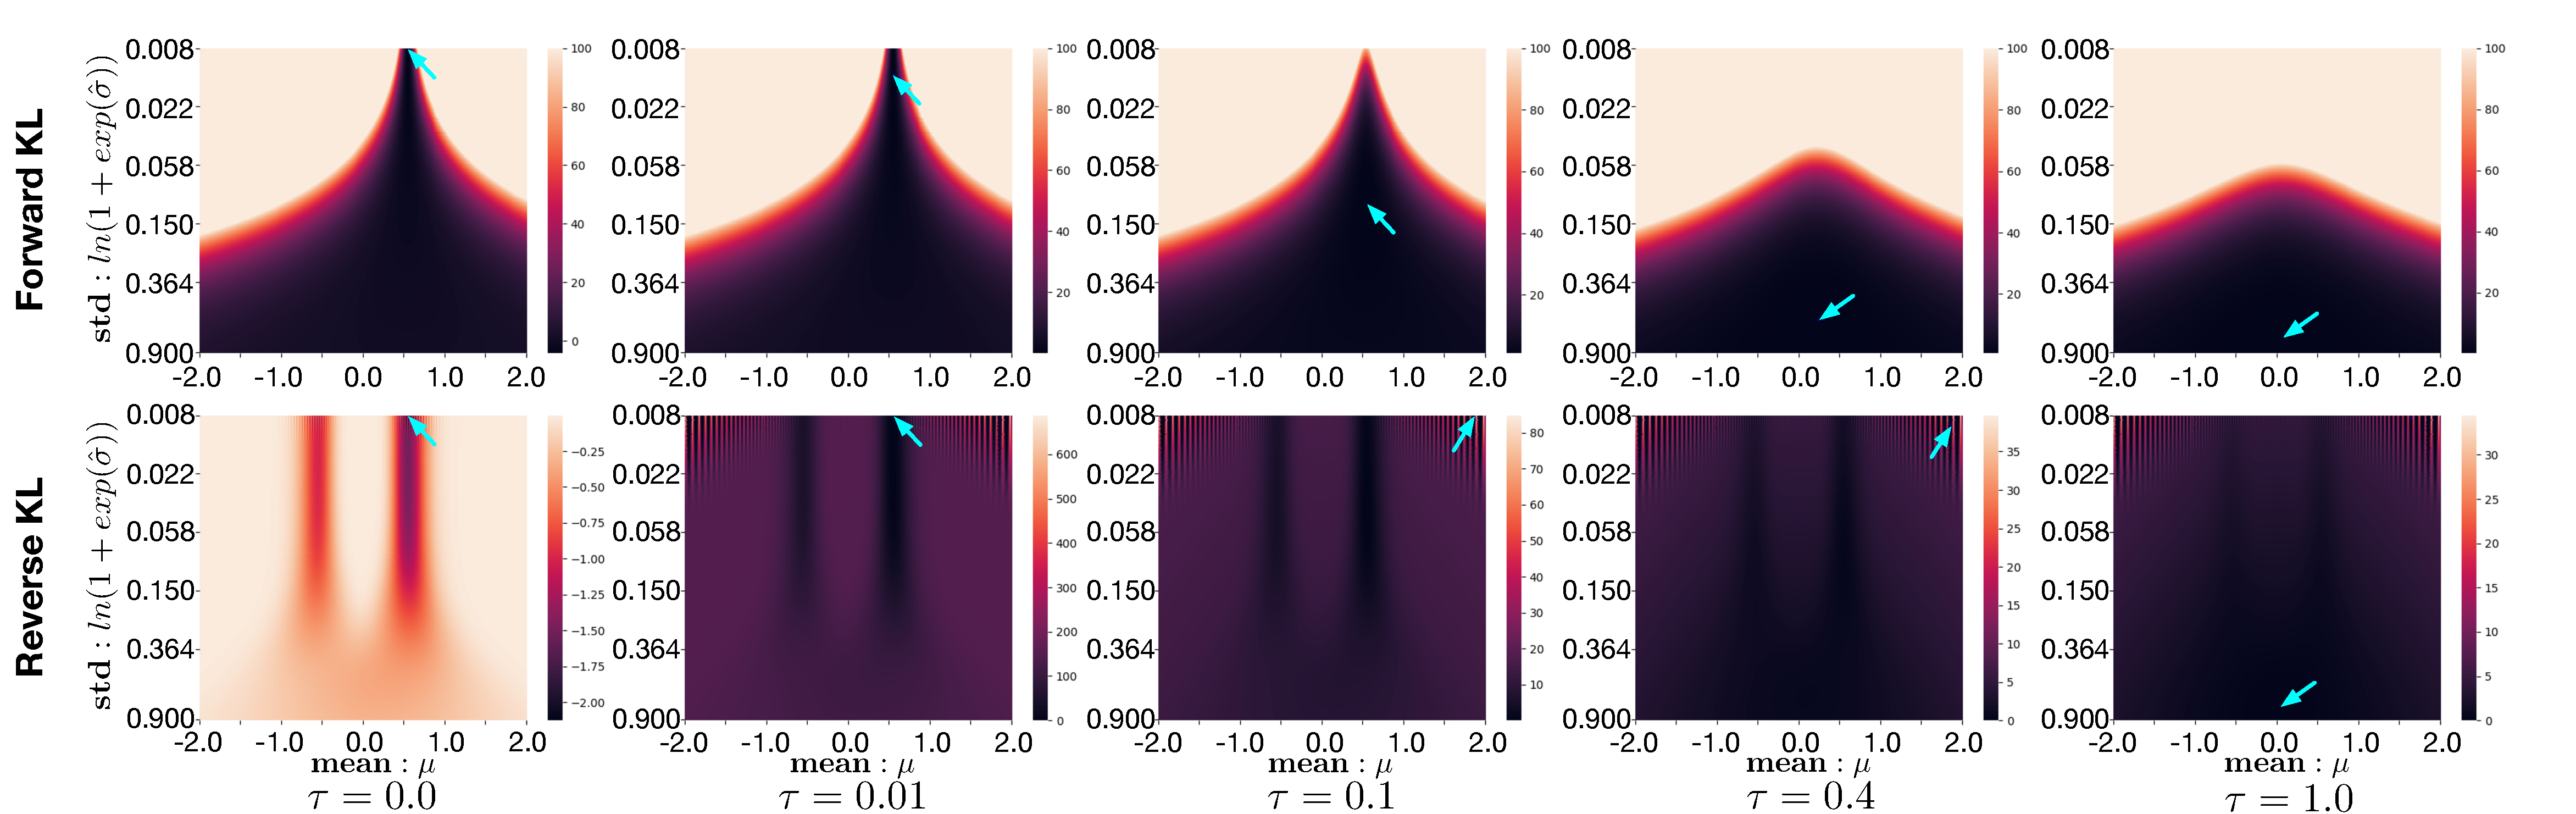
\includegraphics[width=0.99\columnwidth]{figs/bandit/trueQ/heatmaps/heatmap_combined_reduced_pts.pdf}
%     \caption{KL loss over mean and standard deviation across temperature using the Gaussian policy with 128 numerical integration points. }
%     \label{fig:bandit-heatmap-reduced-pts}
% \end{figure}

% \begin{figure}
%     \centering
%     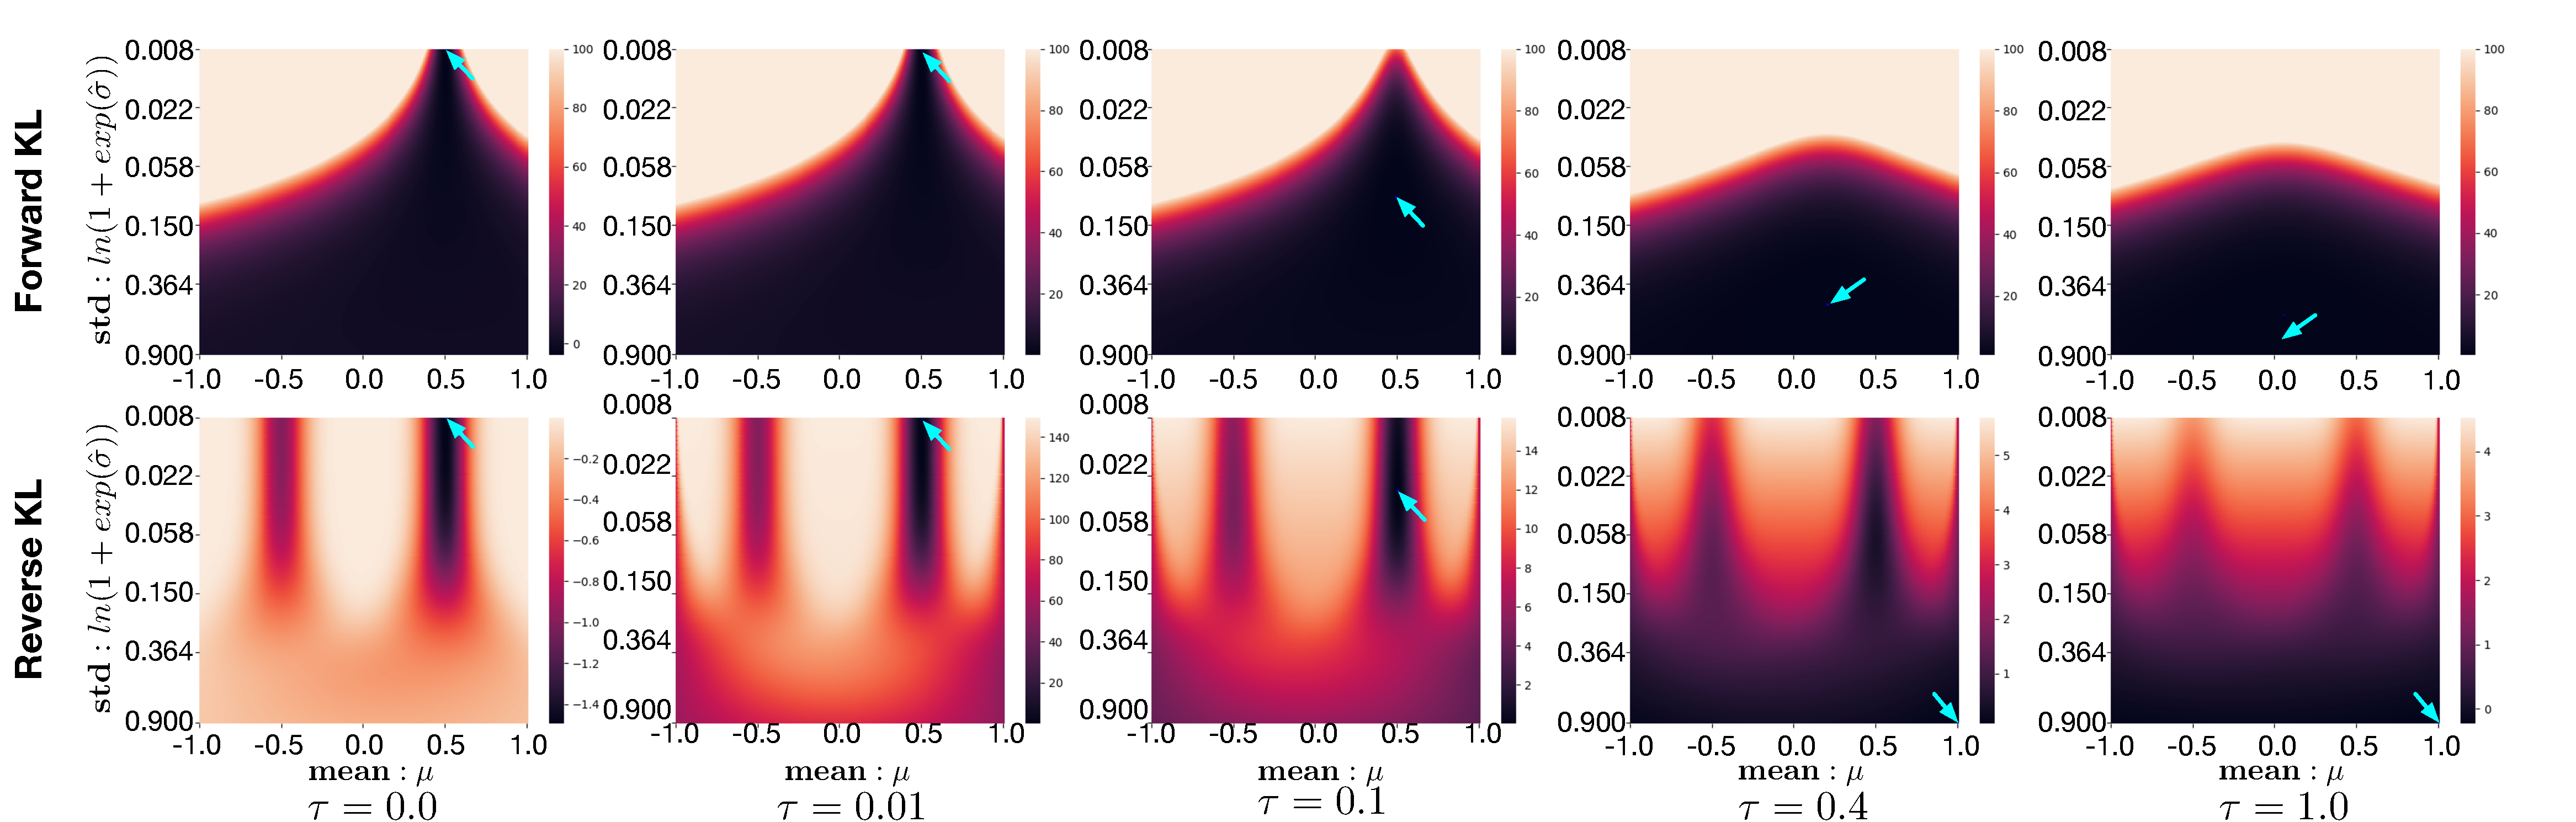
\includegraphics[width=0.99\columnwidth]{figs/bandit/trueQ/heatmaps/heatmap_non_tanh_combined.pdf}
%     \caption{KL loss over mean and standard deviation across temperature using the Gaussian policy without $\tanh$ transformation. Note that the displayed mean range is $[-1,1]$. Different from the previous heatmap, optima are now located at $a=-0.5, 0.5$.  FKL loss has been upper-bounded for better visualization of minima.}
%     \label{fig:bandit-heatmap-non-tanh}
% \end{figure}

% \subsection{Continuous Bandits - Optimization Path}
% Here, we include additional plots for the optimization behaviour of iterates in the continuous bandit. We also include additional summary statistics for the iterates. 

% % \begin{figure}[!ht]
% %   \centering
% %   \begin{subfigure}[b]{0.4\linewidth}
% %     \centering
% %     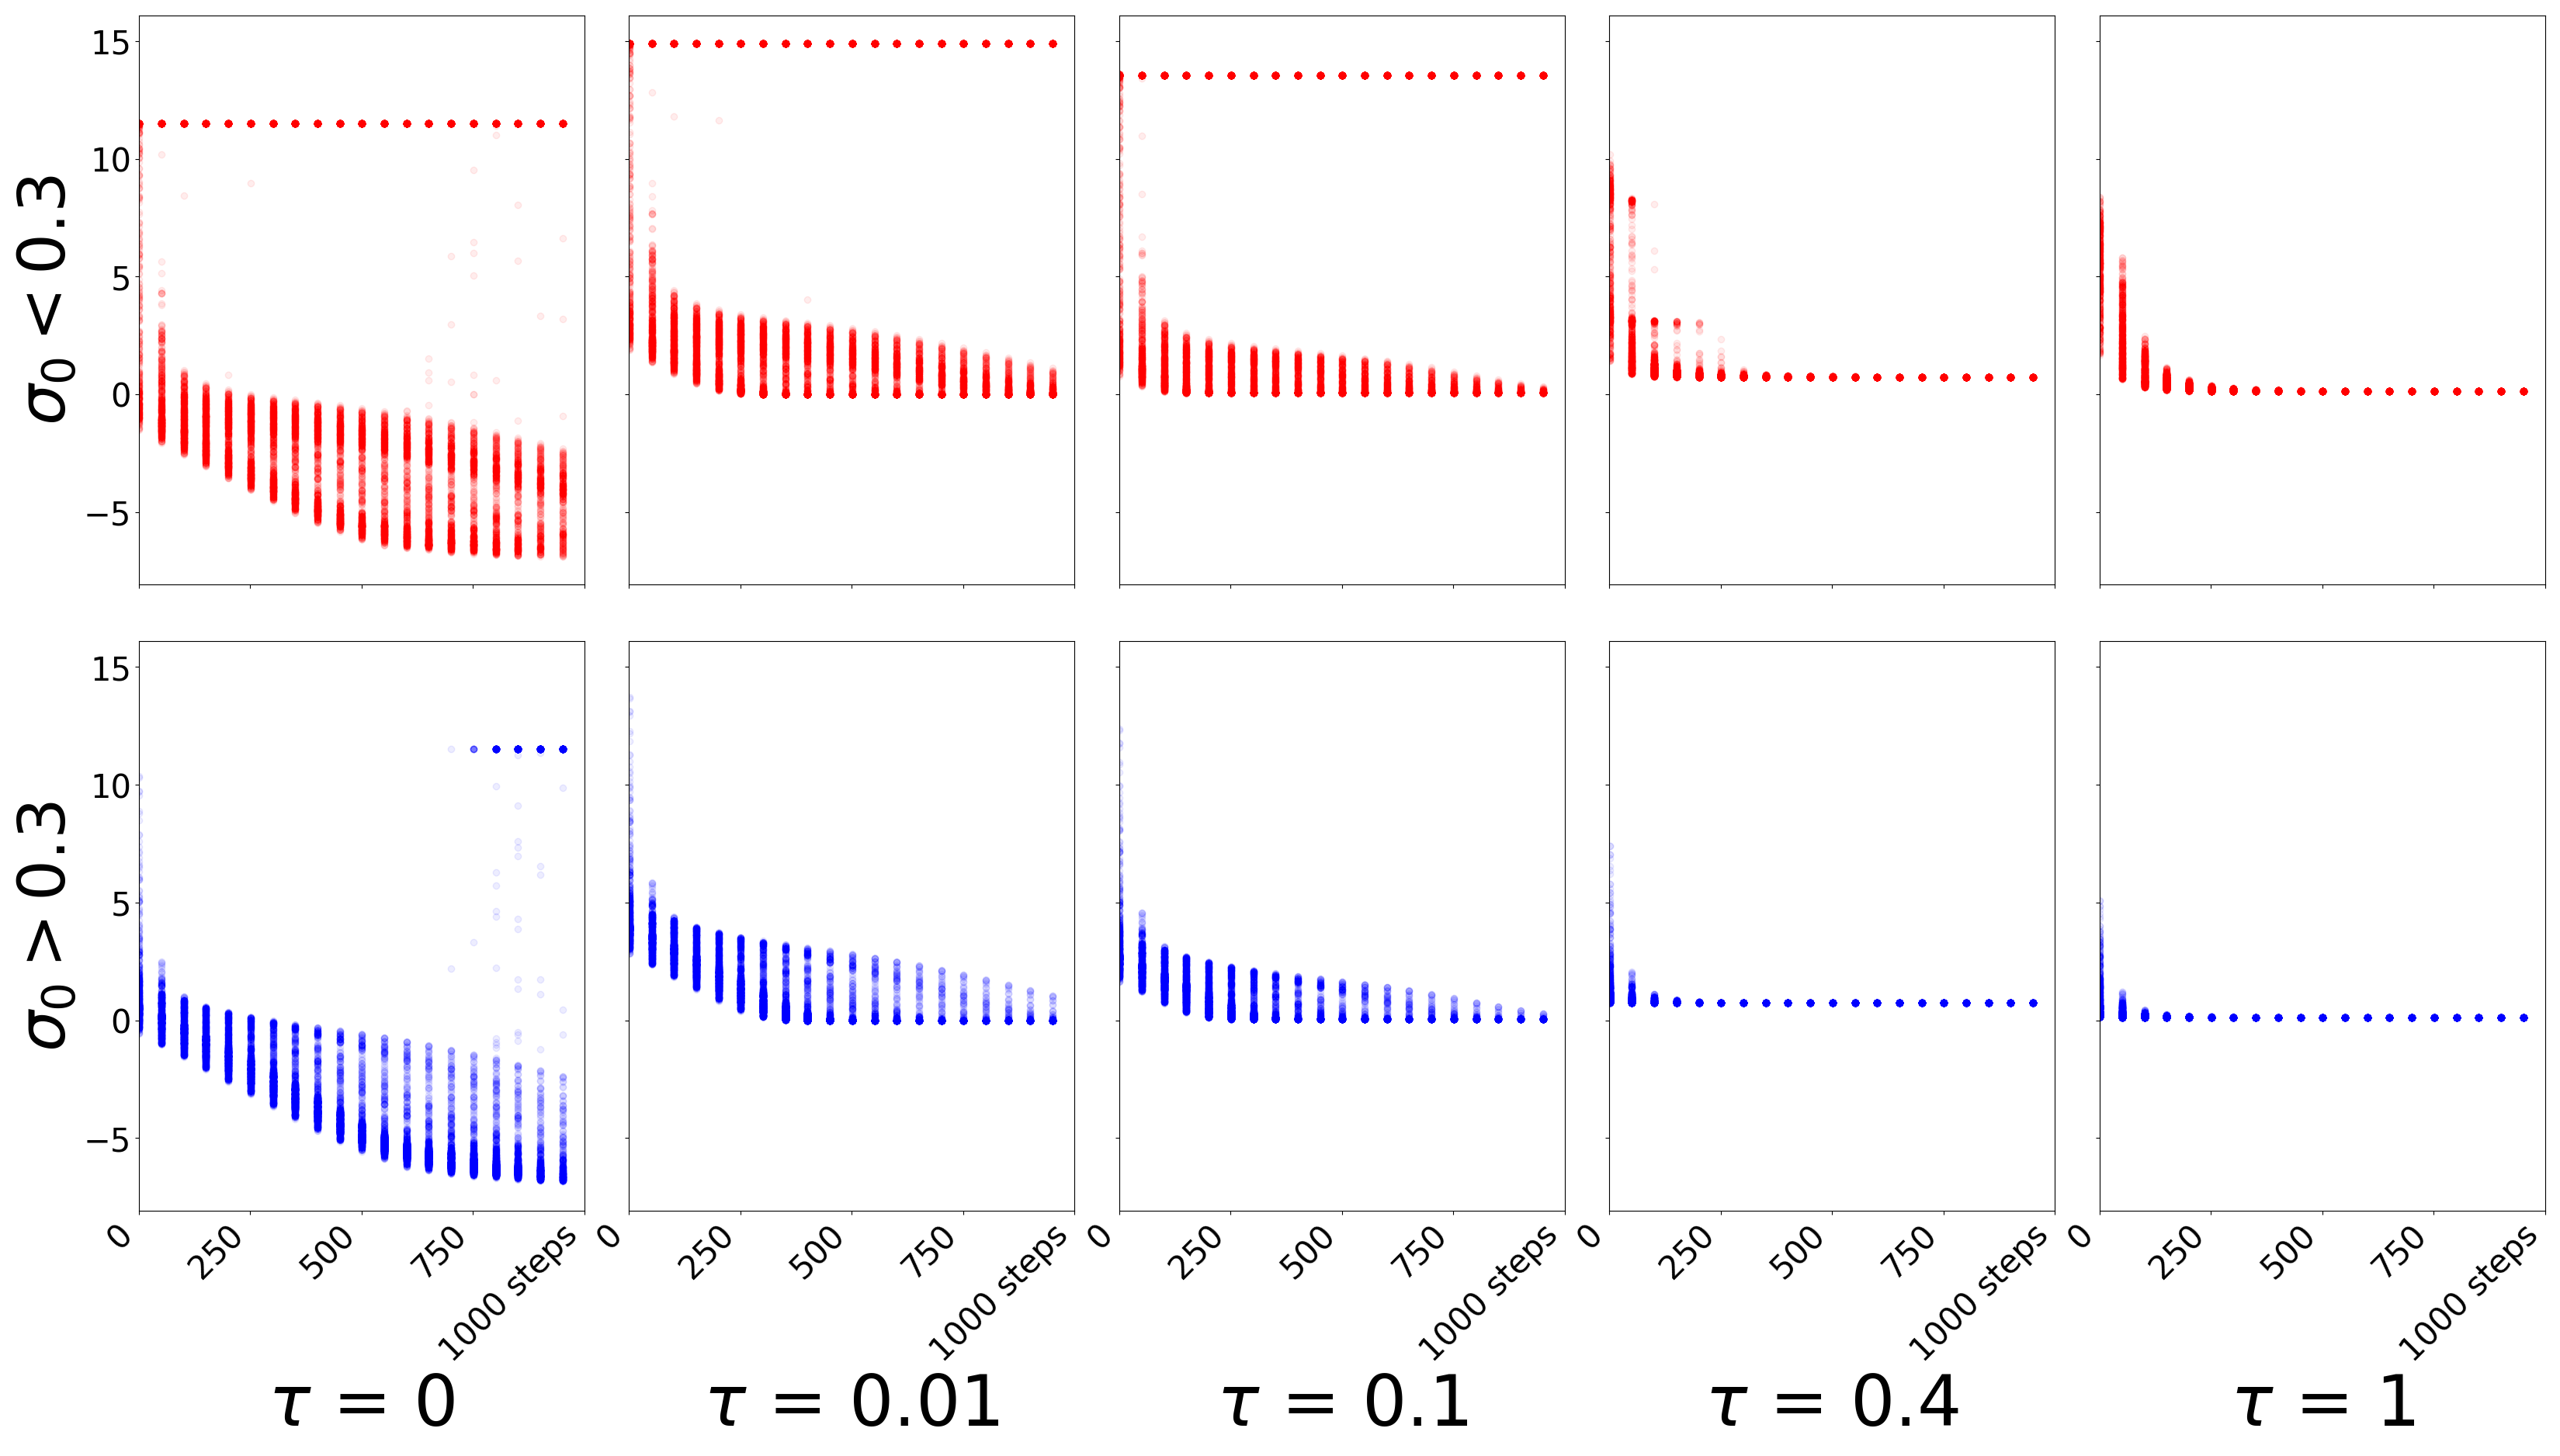
\includegraphics[width=1\columnwidth]{figs/bandit/notlearnQ/modes=1/adam/loss_forward_optim=adam_modes=1_lr=0.01.png}
% %     \caption{Forward KL, Adam.}
% %     \label{fig:bandit-loss-forward-adam}
% %   \end{subfigure}%
% %   \begin{subfigure}[b]{0.4\linewidth}
% %     \centering
% %     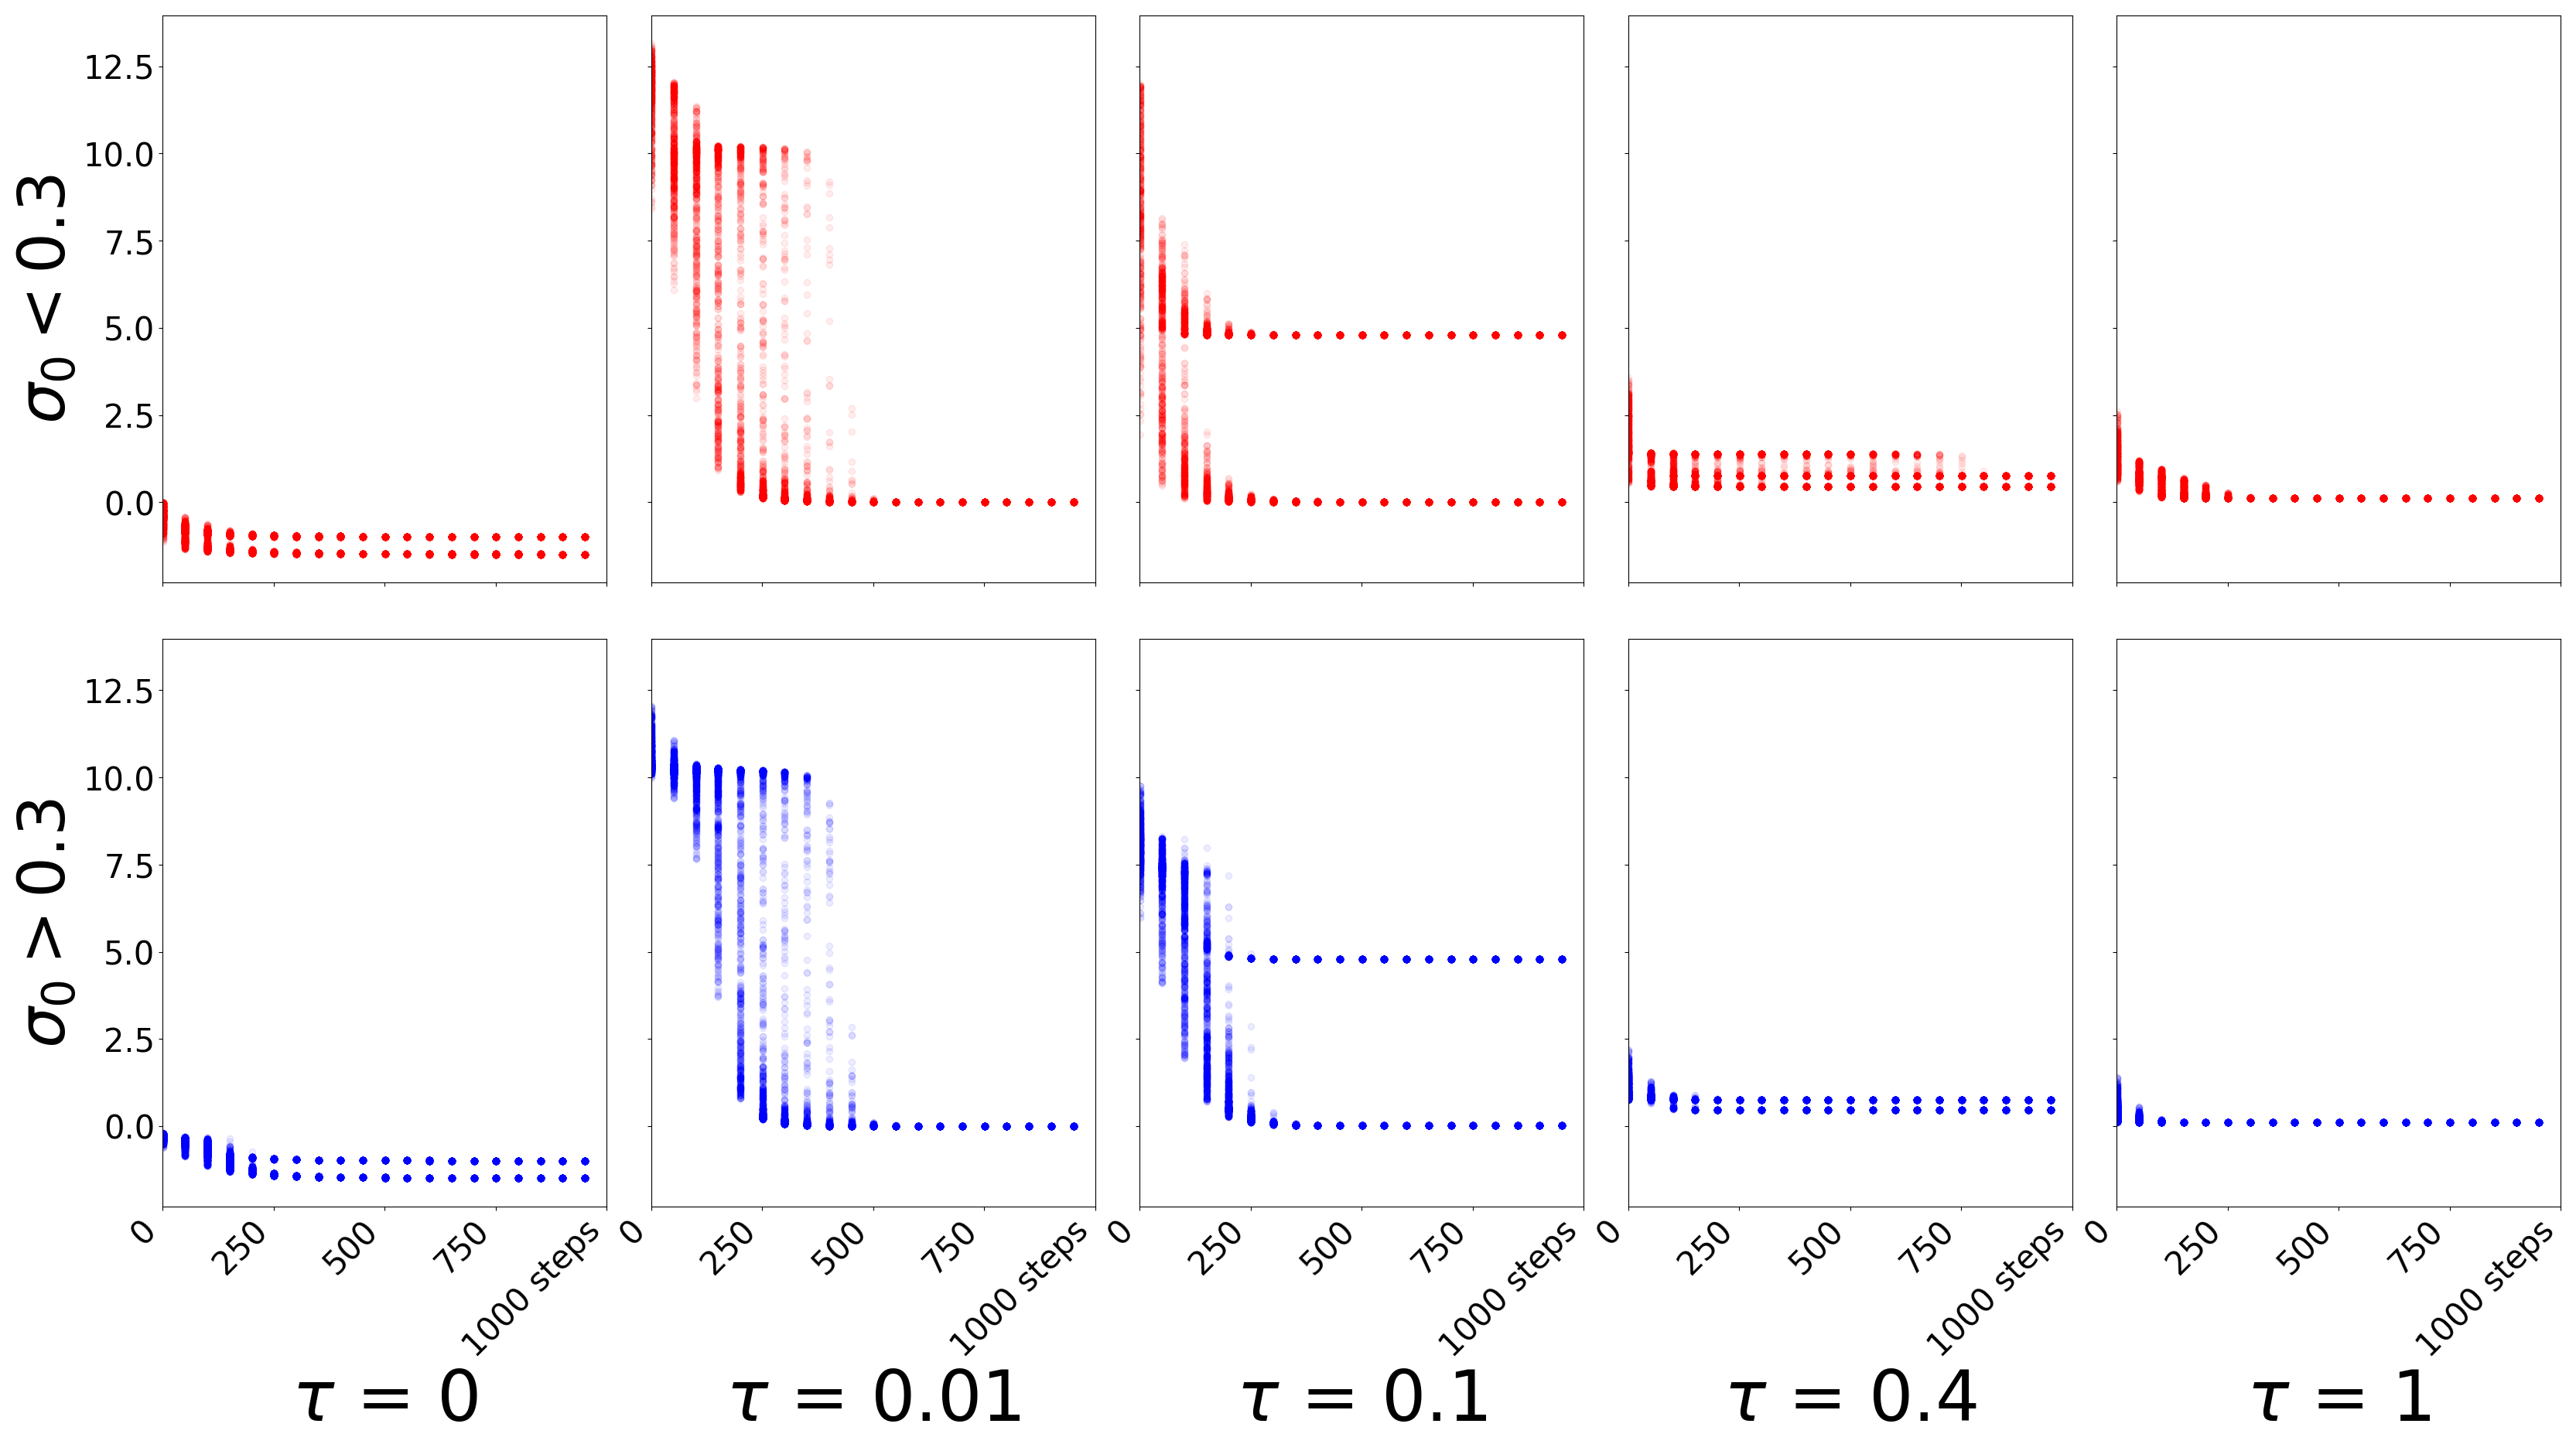
\includegraphics[width=1\columnwidth]{figs/bandit/notlearnQ/modes=1/adam/loss_reverse_optim=adam_modes=1_lr=0.01.png}
% %     \caption{Reverse KL, Adam. }
% %     \label{fig:bandit-loss-reverse-adam}
% %   \end{subfigure}
  
% %   \begin{subfigure}[b]{0.4\linewidth}
% %     \centering
% %     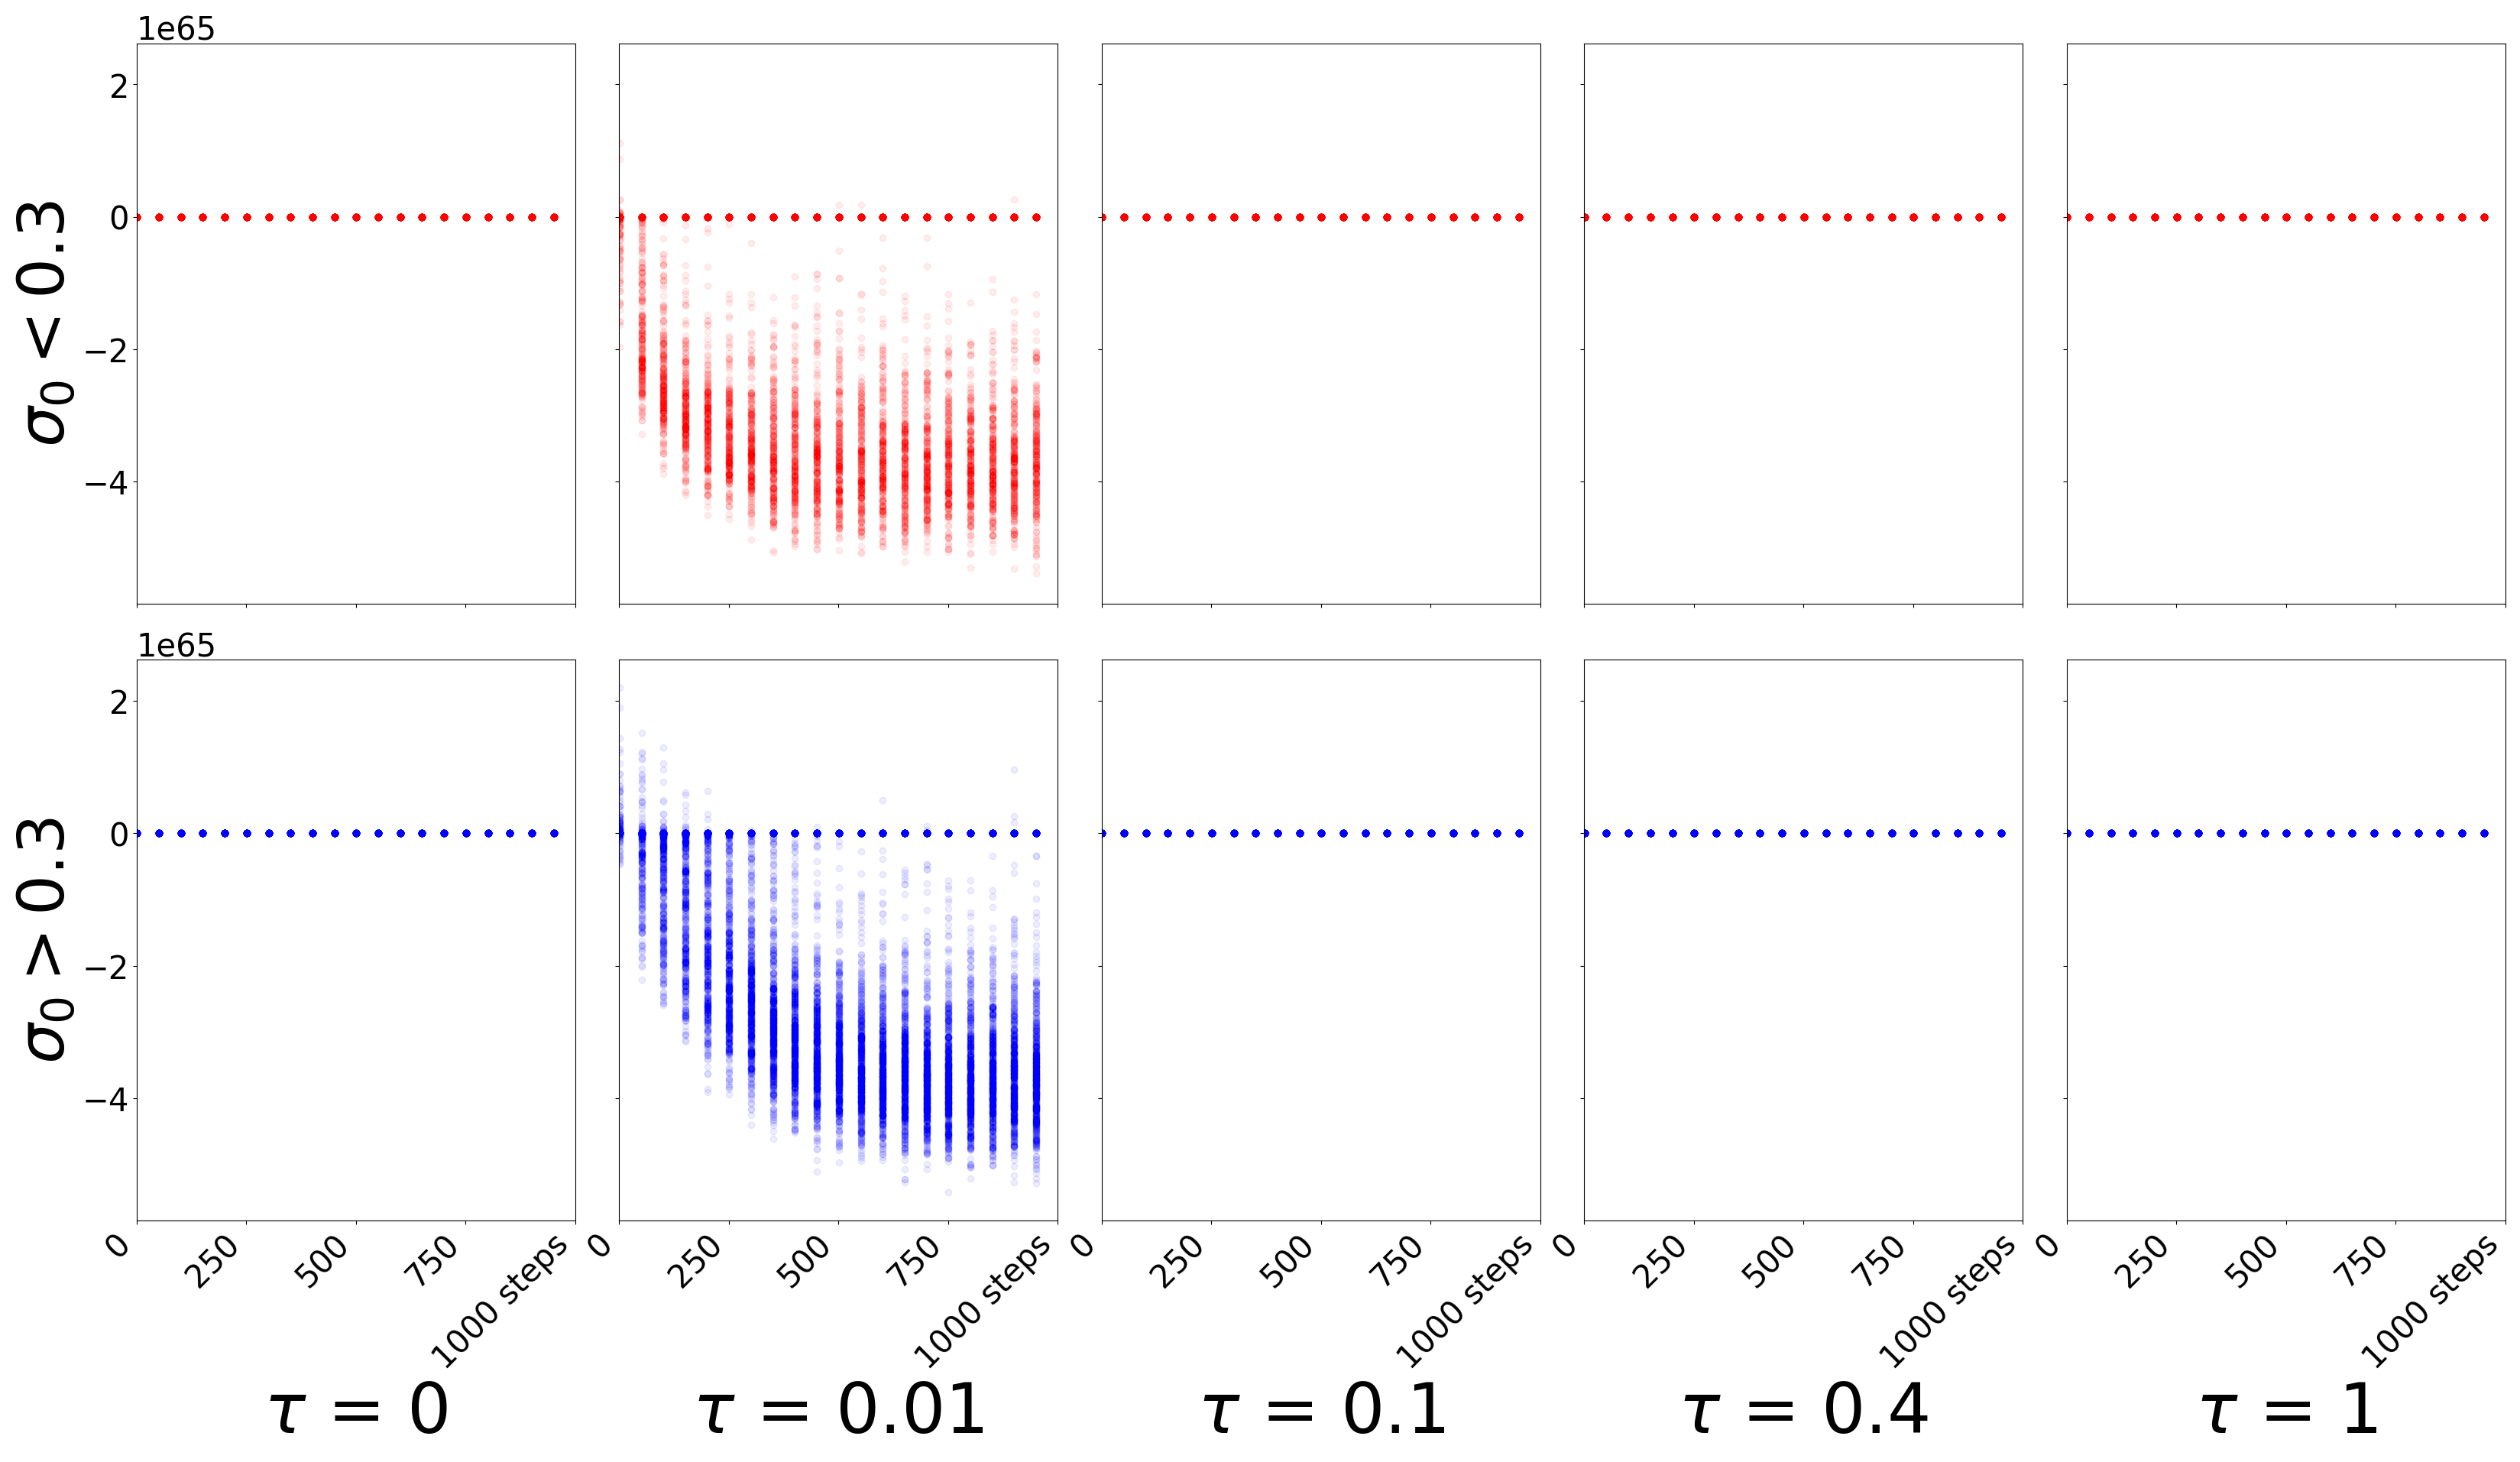
\includegraphics[width=1\columnwidth]{figs/bandit/notlearnQ/modes=1/rmsprop/loss_forward_optim=rmsprop_modes=1_lr=0.01.png}
% %     \caption{Forward KL, RMSprop.}
% %     \label{fig:bandit-loss-forward-rmsprop}
% %   \end{subfigure}%
% %   \begin{subfigure}[b]{0.4\linewidth}
% %     \centering
% %     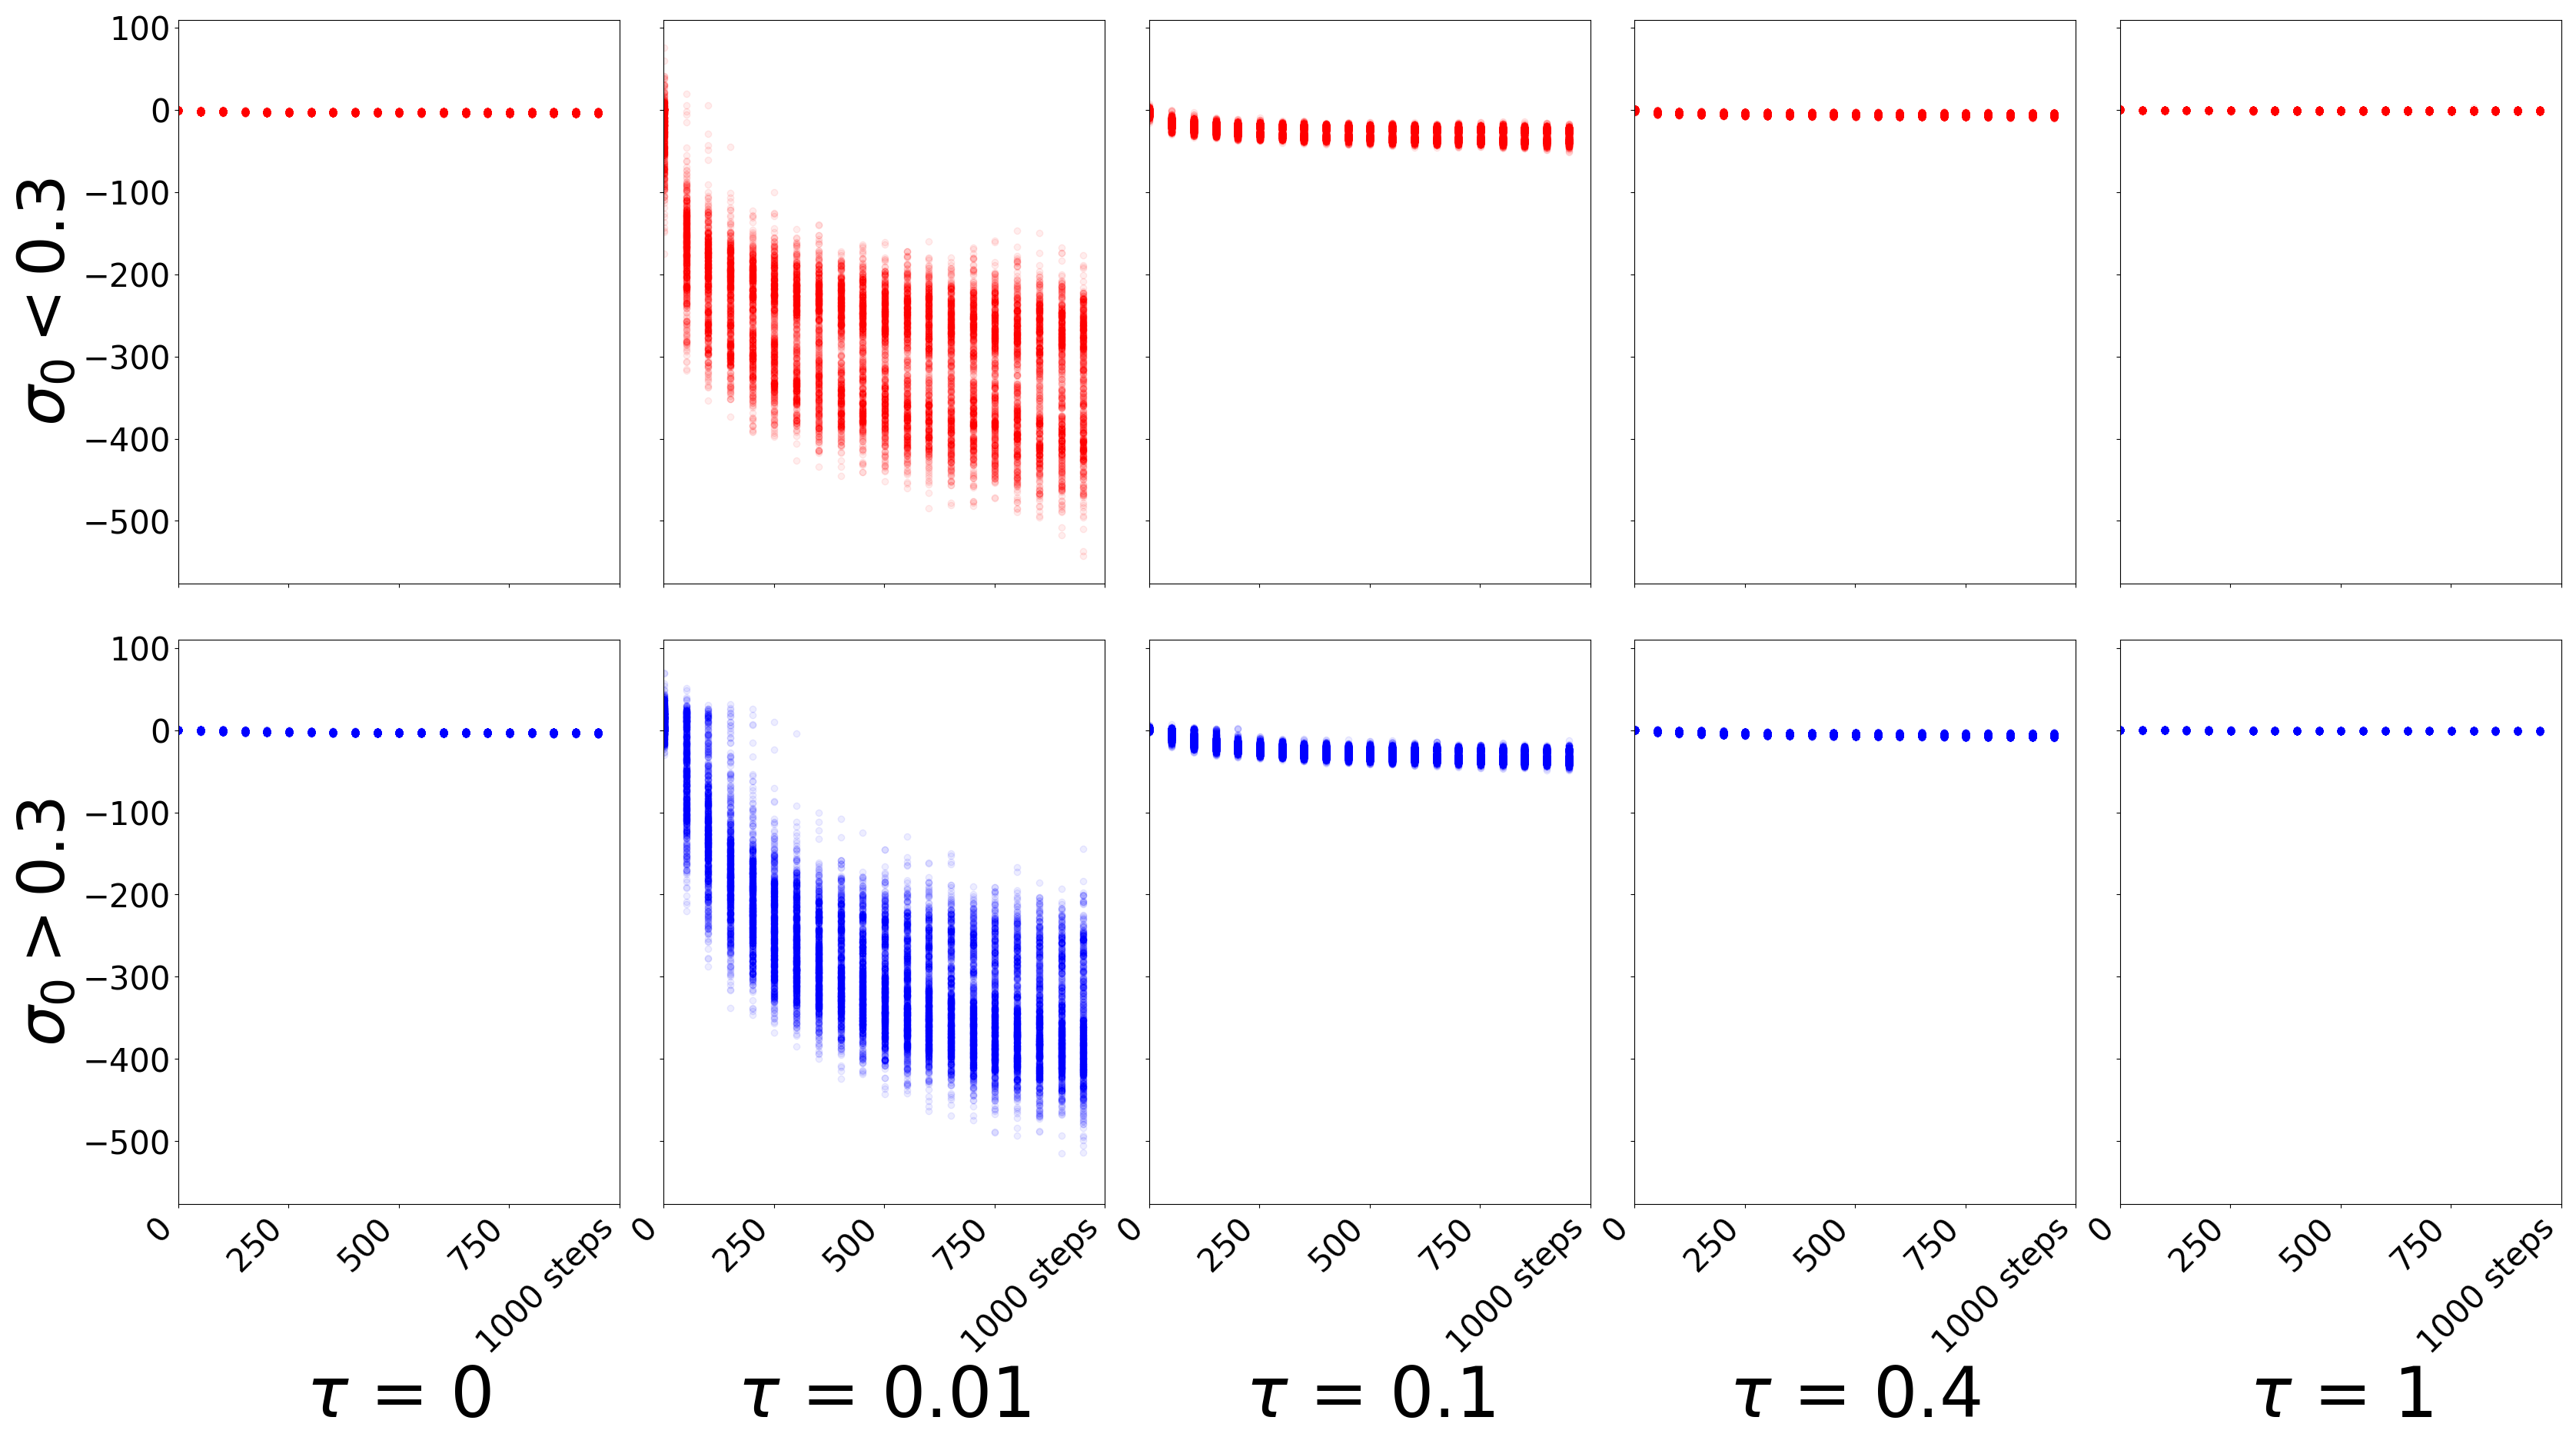
\includegraphics[width=1\columnwidth]{figs/bandit/notlearnQ/modes=1/rmsprop/loss_reverse_optim=rmsprop_modes=1_lr=0.01.png}
% %     \caption{Reverse KL, RMSprop.}
% %     \label{fig:bandit-loss-reverse-rmsprop}
% %   \end{subfigure}
  
% %   \begin{subfigure}[b]{0.4\linewidth}
% %     \centering
% %     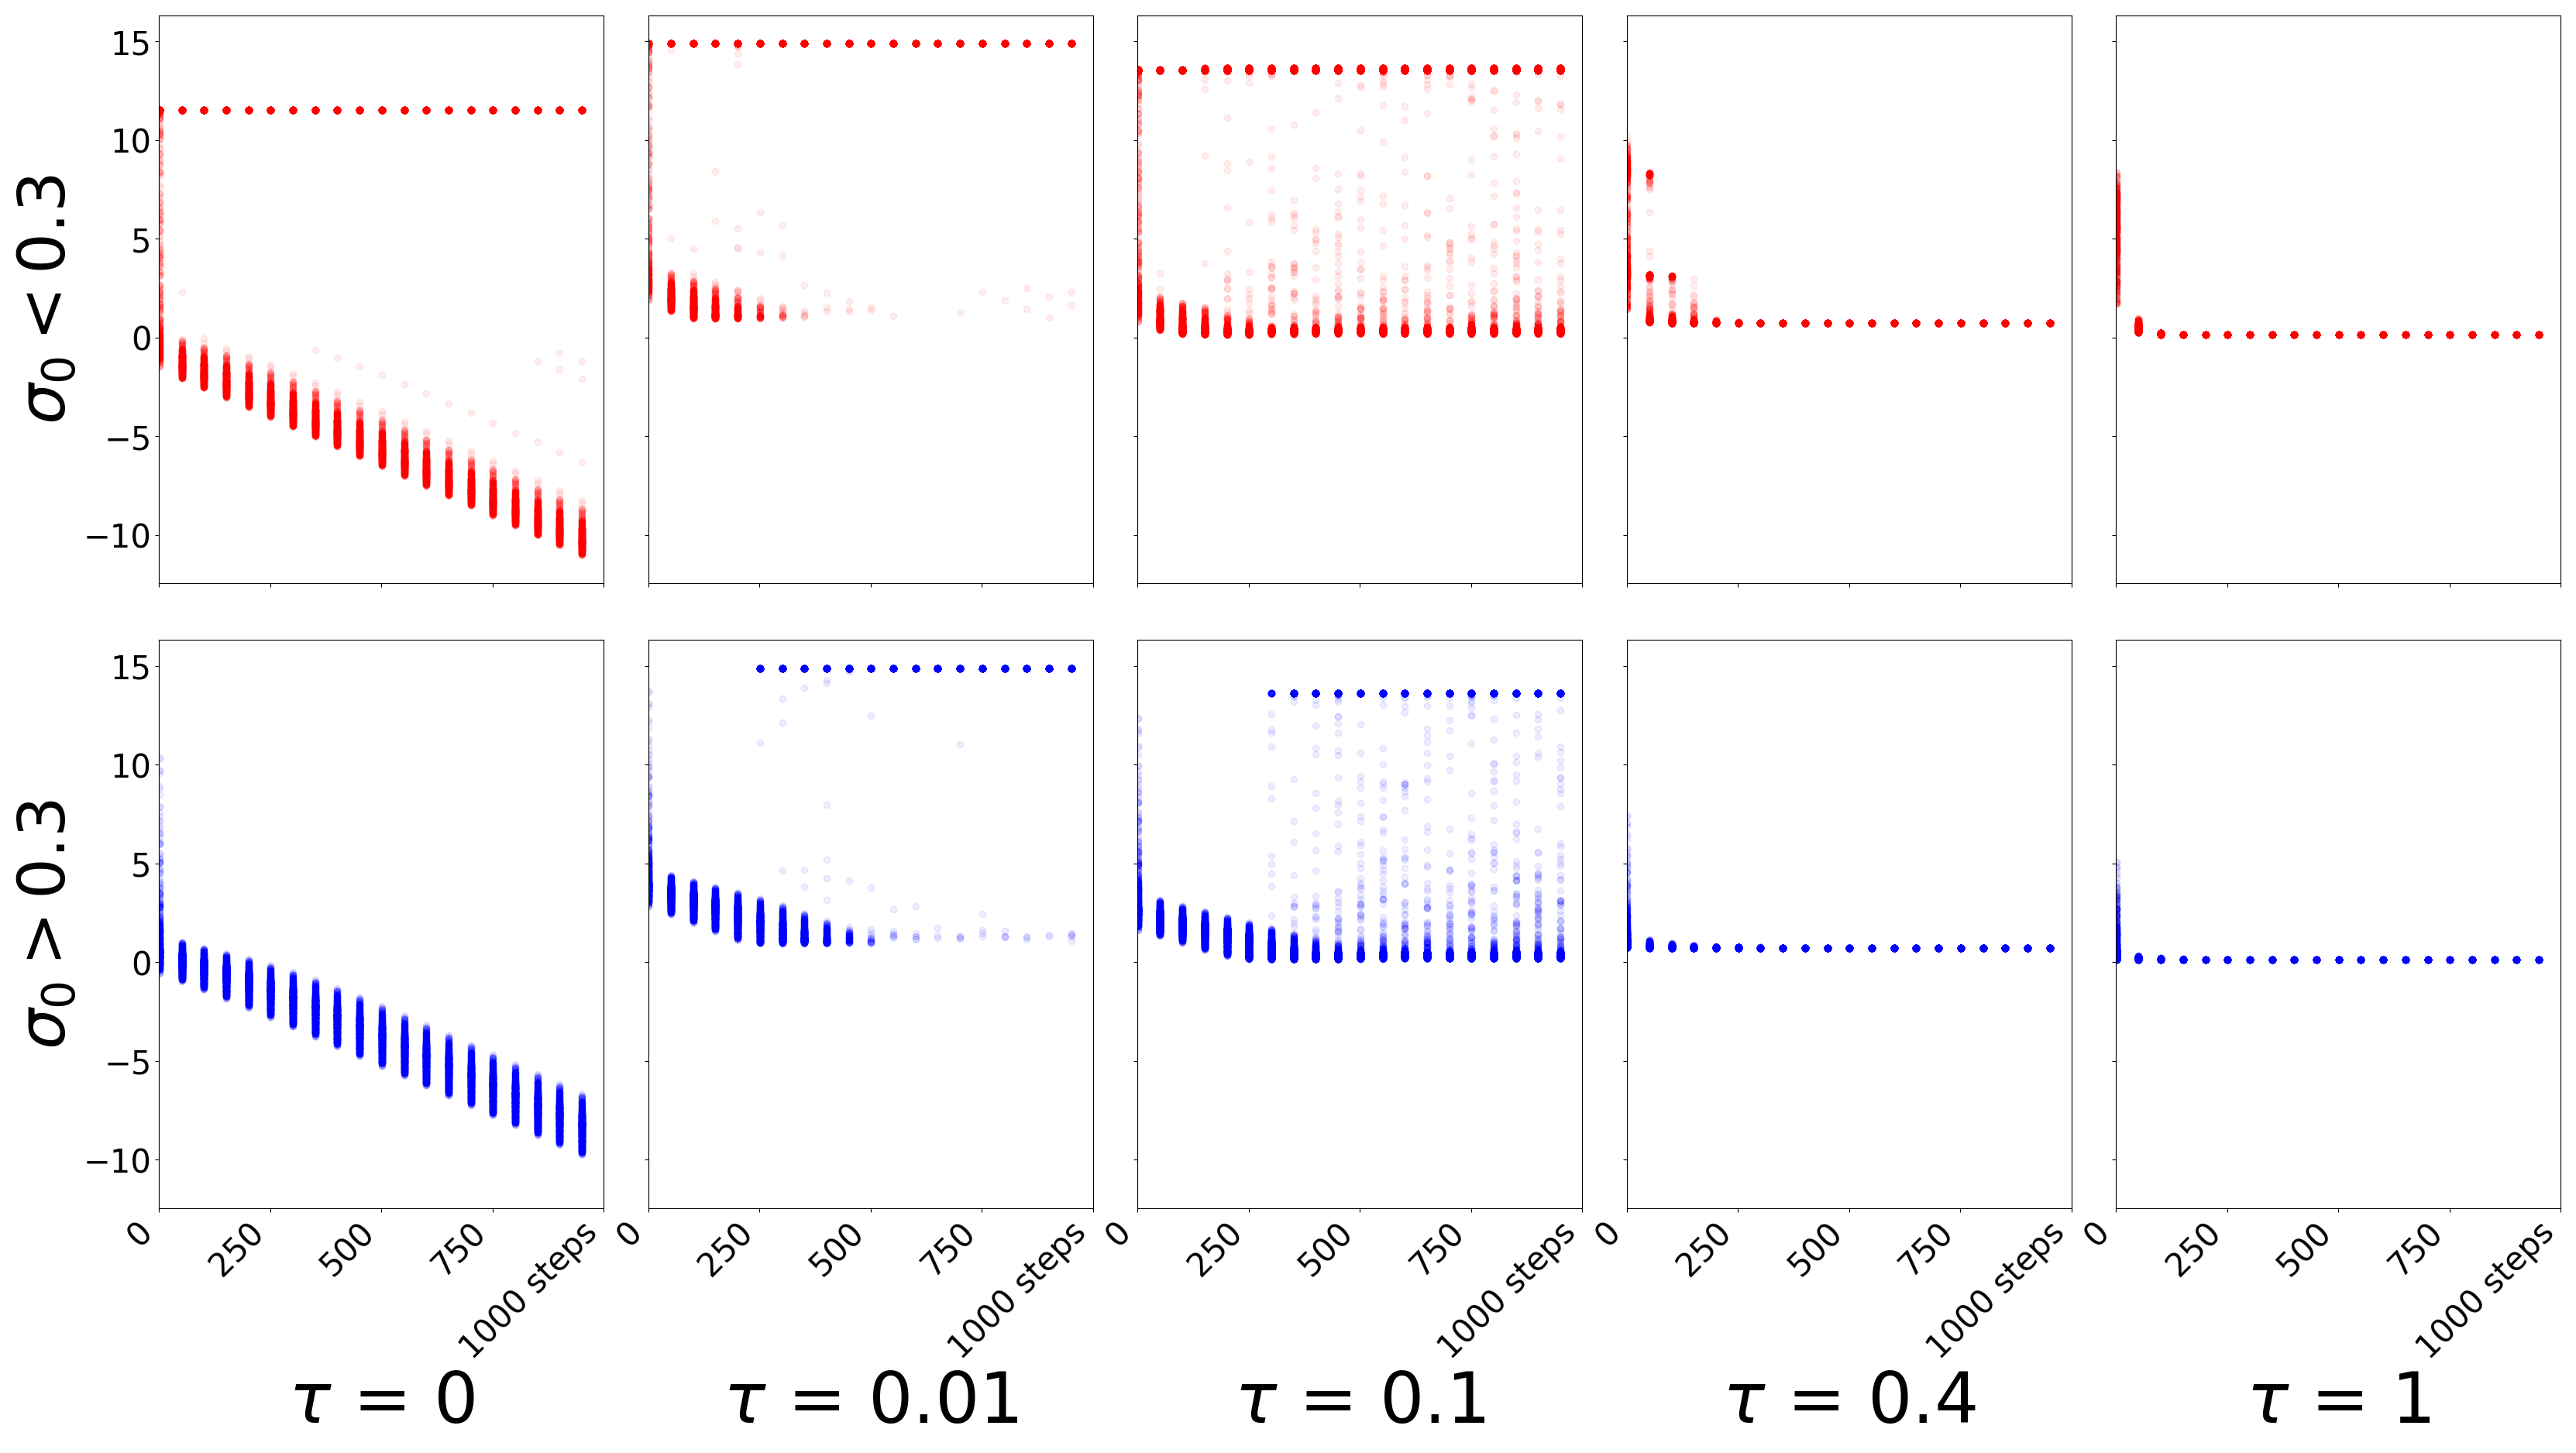
\includegraphics[width=1\columnwidth]{figs/bandit/notlearnQ/modes=1/sgd/loss_forward_optim=sgd_modes=1_lr=0.01.png}
% %     \caption{Forward KL, SGD.}
% %     \label{fig:bandit-loss-forward-sgd}
% %   \end{subfigure}%
% %   \begin{subfigure}[b]{0.4\linewidth}
% %     \centering
% %     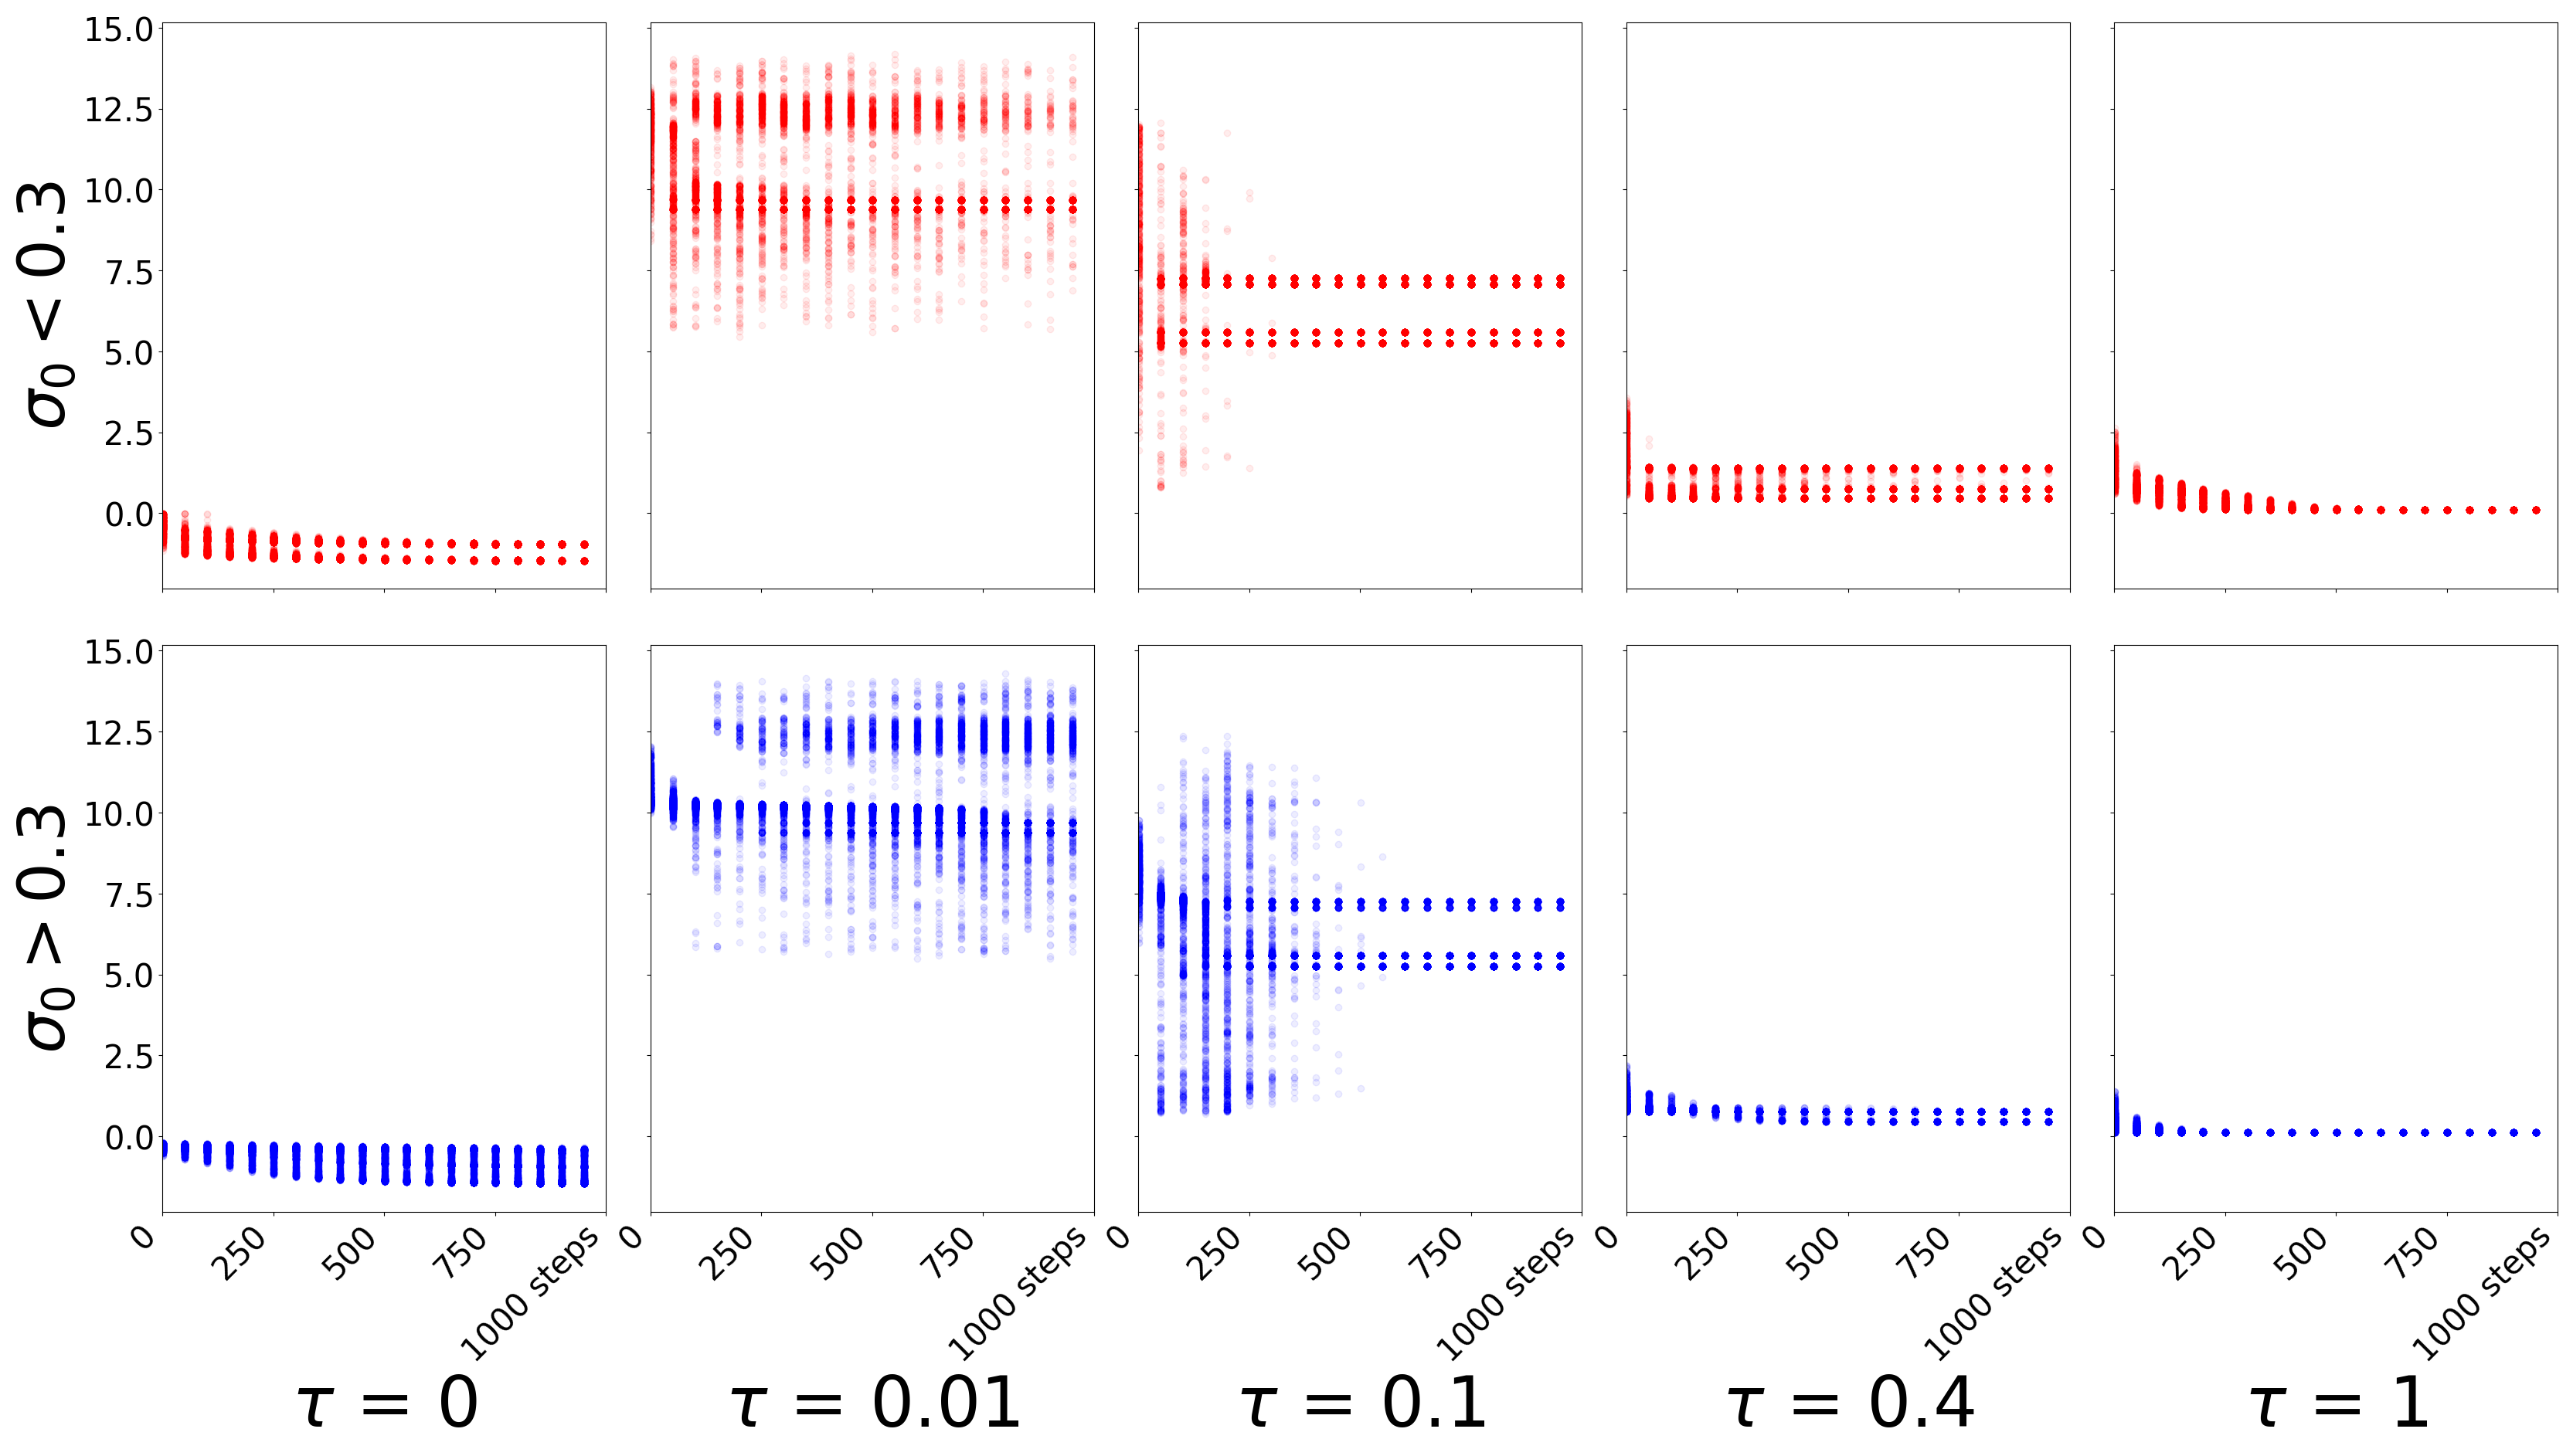
\includegraphics[width=1\columnwidth]{figs/bandit/notlearnQ/modes=1/sgd/loss_reverse_optim=sgd_modes=1_lr=0.01.png}
% %     \caption{Reverse KL, SGD.}
% %     \label{fig:bandit-loss-reverse-sgd}
% %   \end{subfigure}
% %   \caption{Loss over time with unimodal policy. }
% % \end{figure}

% \begin{figure}[!ht]
%   \centering
%   \begin{subfigure}[b]{0.4\linewidth}
%     \centering
%     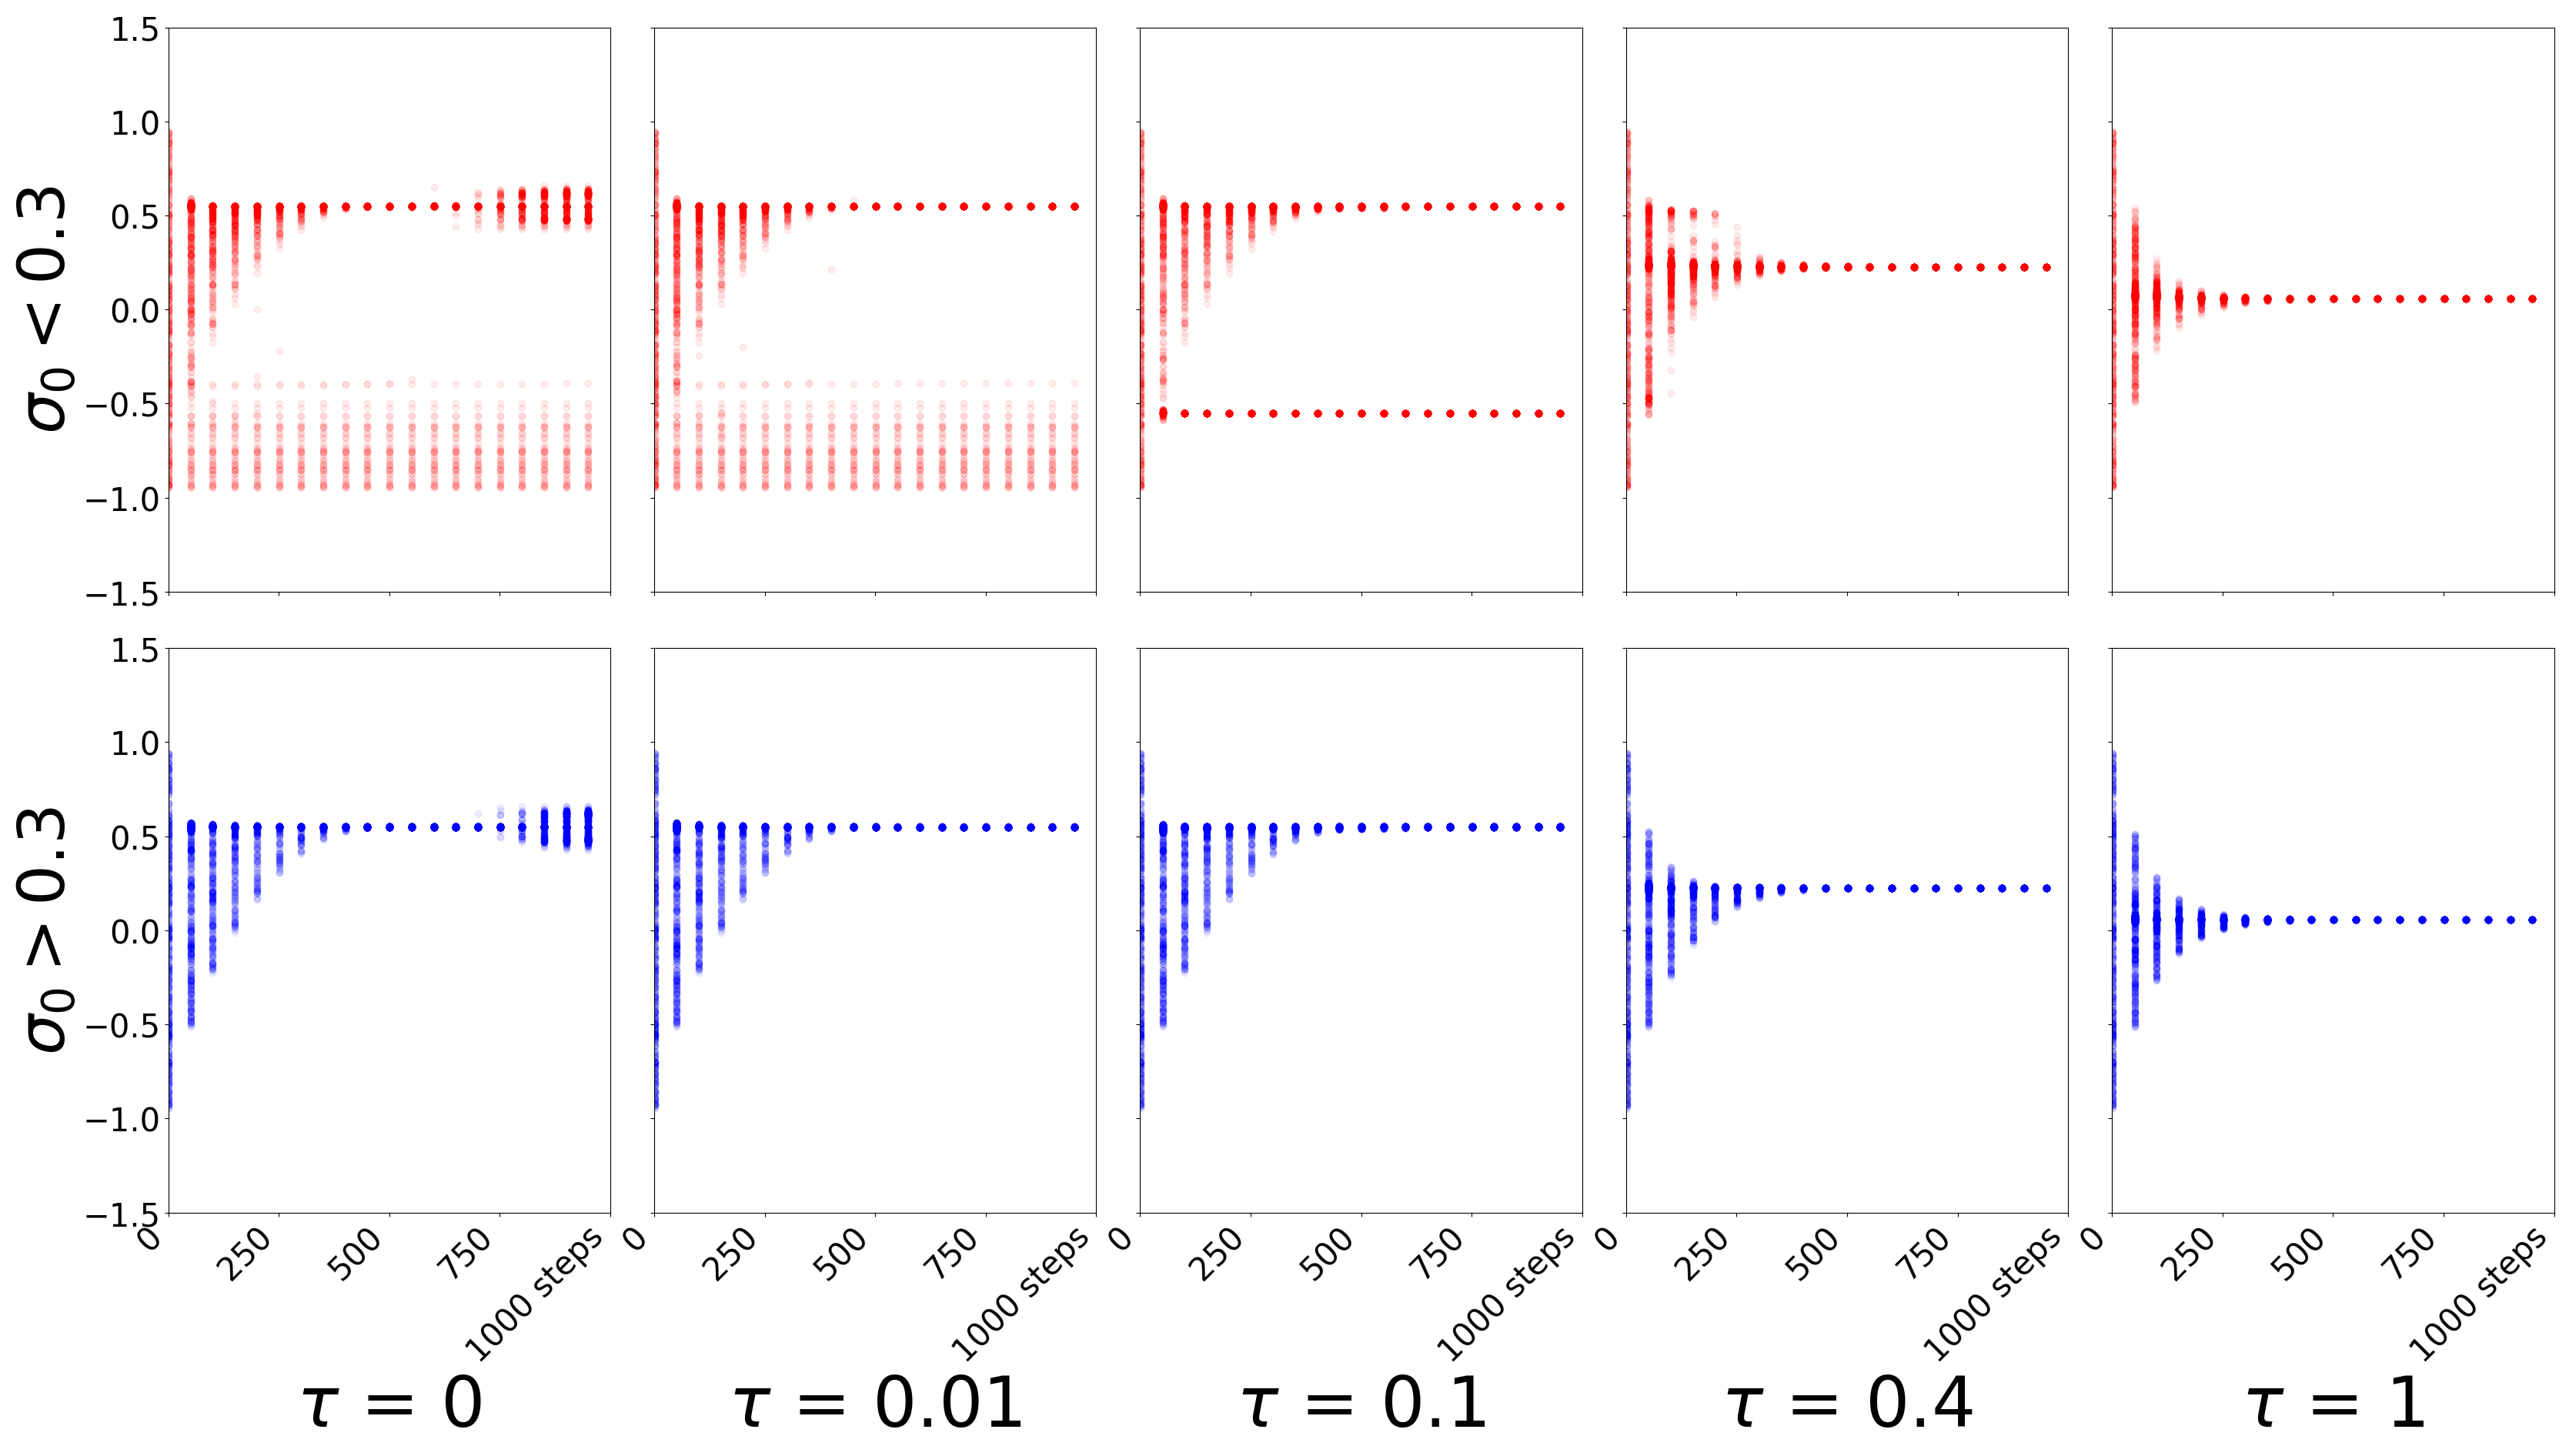
\includegraphics[width=1\columnwidth]{figs/bandit/notlearnQ/modes=1/adam/mean_forward_optim=adam_modes=1_lr=0.01.png}
%     \caption{Forward KL, Adam.}
%     \label{fig:bandit-mean-forward-adam}
%   \end{subfigure}%
%   \begin{subfigure}[b]{0.4\linewidth}
%     \centering
%     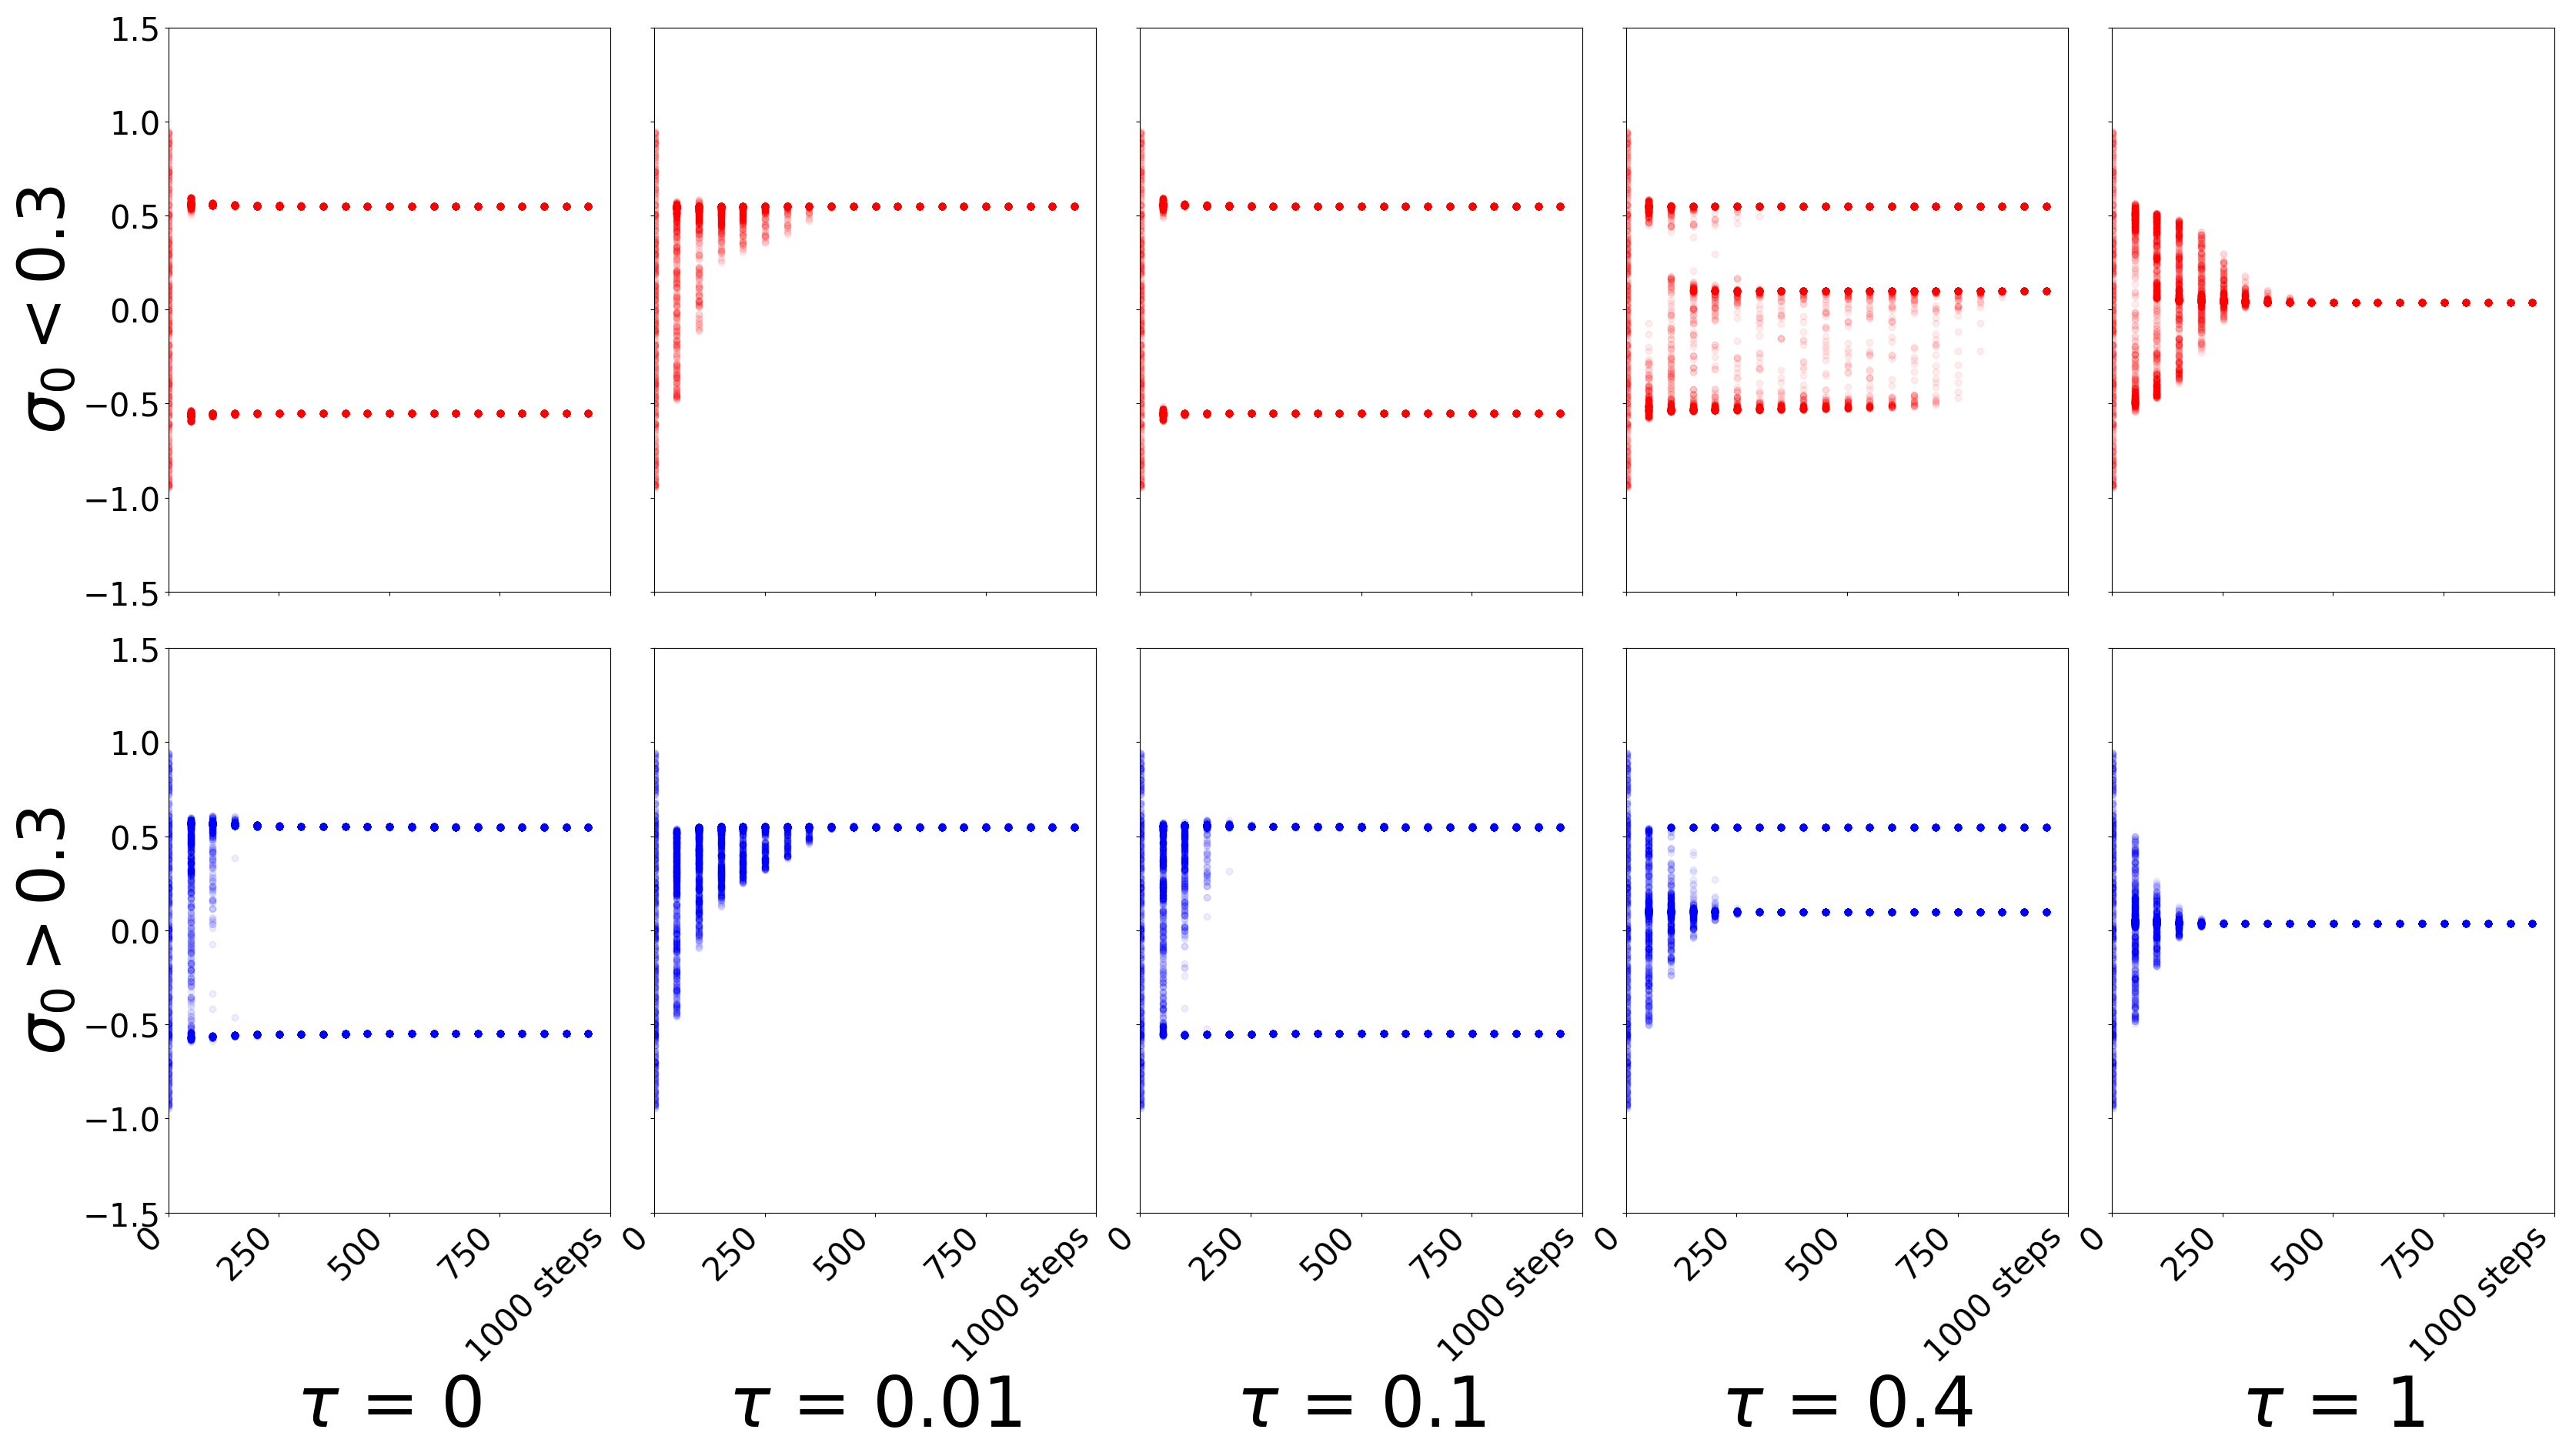
\includegraphics[width=1\columnwidth]{figs/bandit/notlearnQ/modes=1/adam/mean_reverse_optim=adam_modes=1_lr=0.01.png}
%     \caption{Reverse KL, Adam. }
%     \label{fig:bandit-mean-reverse-adam}
%   \end{subfigure}
  
%   \begin{subfigure}[b]{0.4\linewidth}
%     \centering
%     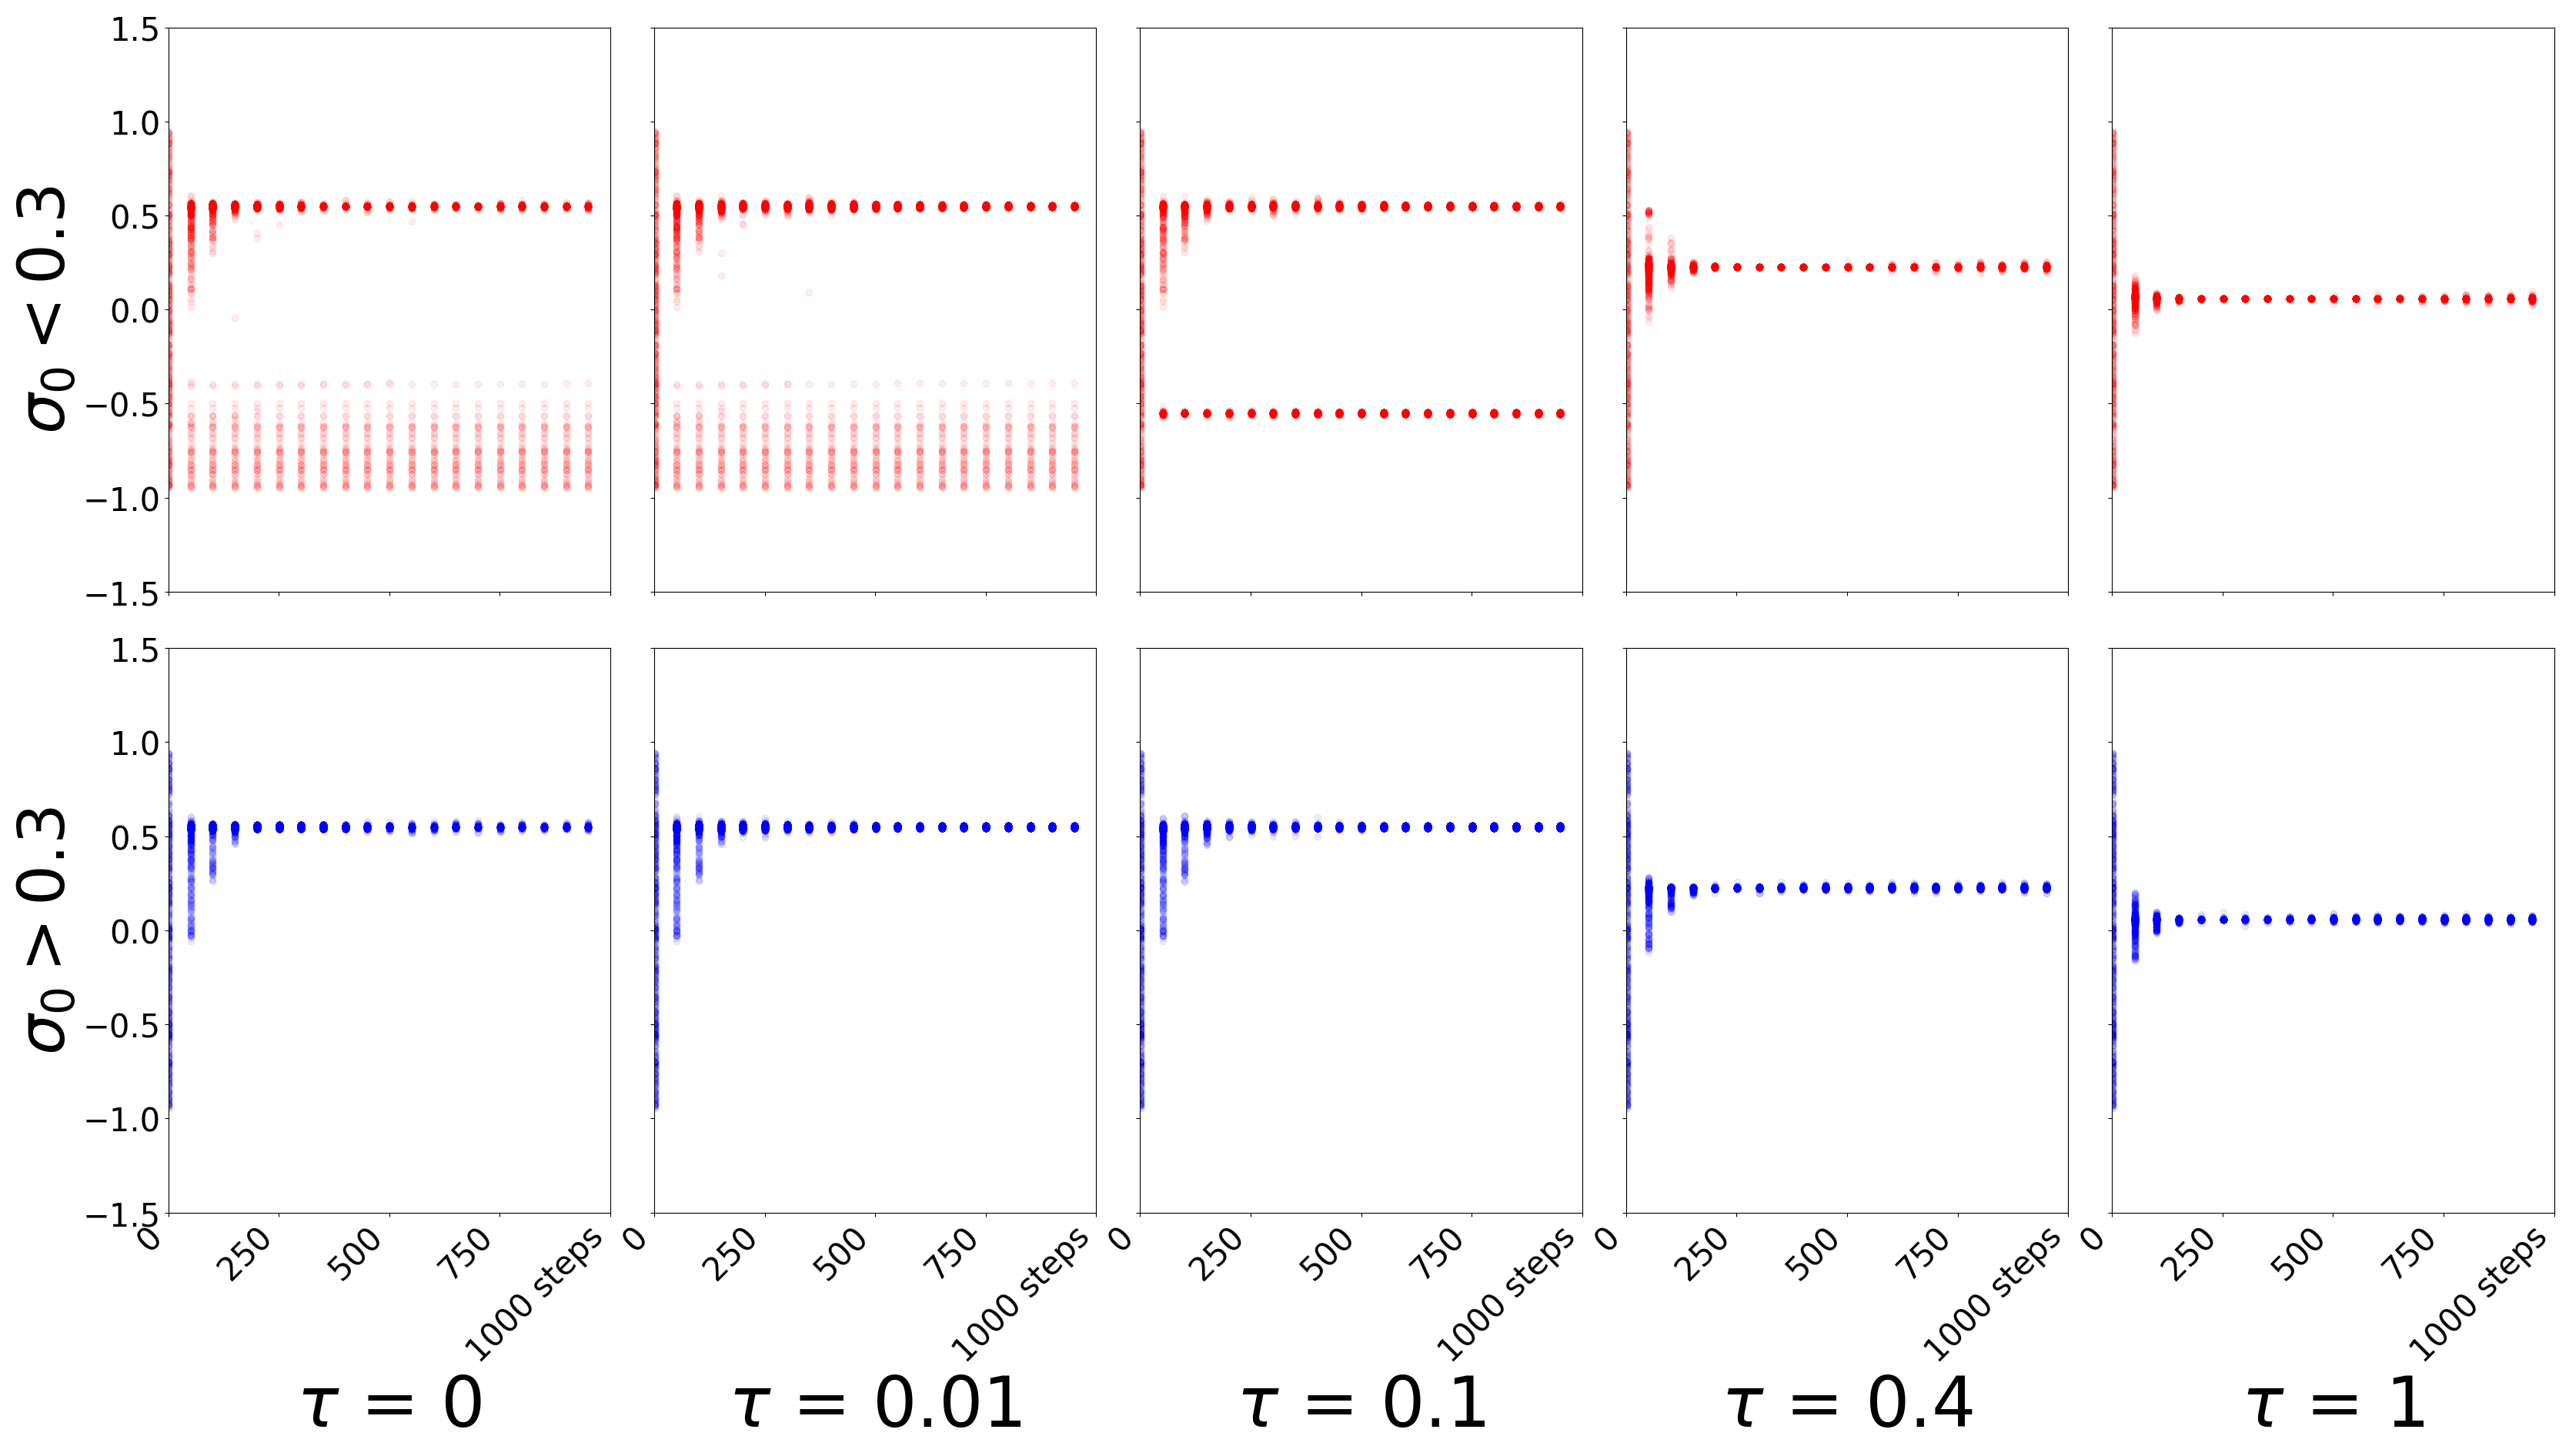
\includegraphics[width=1\columnwidth]{figs/bandit/notlearnQ/modes=1/rmsprop/mean_forward_optim=rmsprop_modes=1_lr=0.01.png}
%     \caption{Forward KL, RMSprop.}
%     \label{fig:bandit-mean-forward-rmsprop}
%   \end{subfigure}%
%   \begin{subfigure}[b]{0.4\linewidth}
%     \centering
%     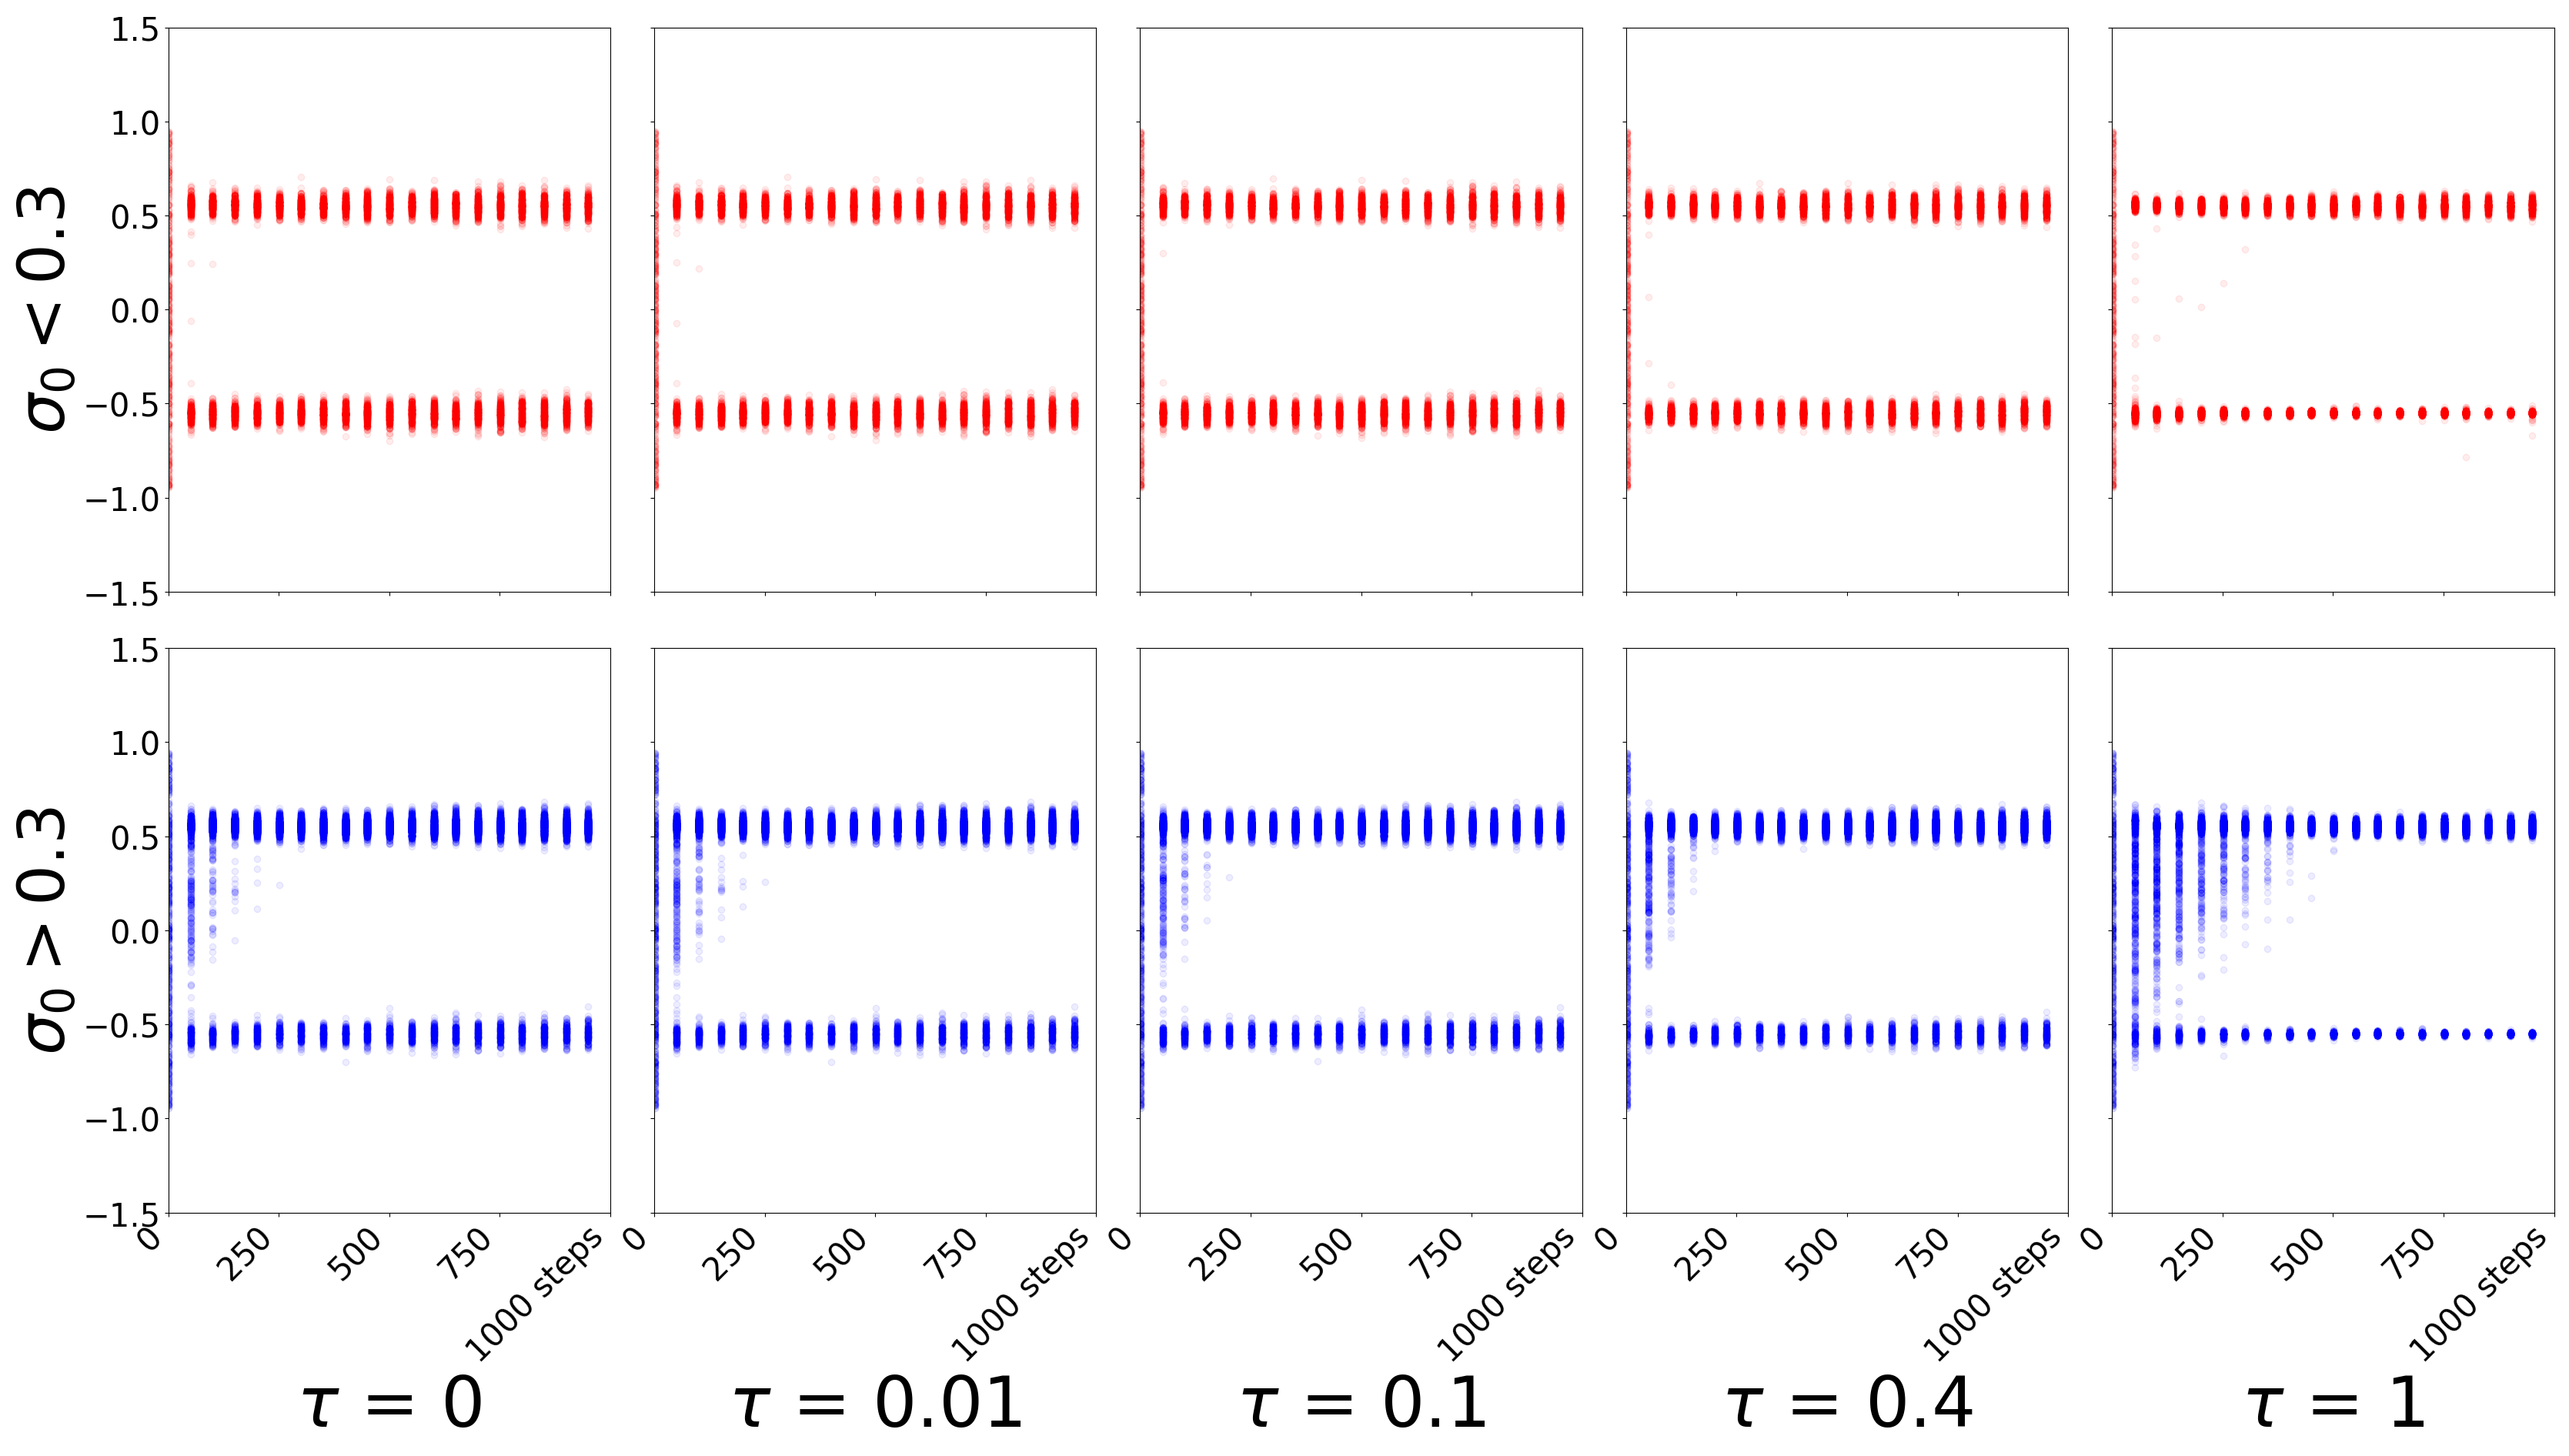
\includegraphics[width=1\columnwidth]{figs/bandit/notlearnQ/modes=1/rmsprop/mean_reverse_optim=rmsprop_modes=1_lr=0.01.png}
%     \caption{Reverse KL, RMSprop.}
%     \label{fig:bandit-mean-reverse-rmsprop}
%   \end{subfigure}
  
%   \begin{subfigure}[b]{0.4\linewidth}
%     \centering
%     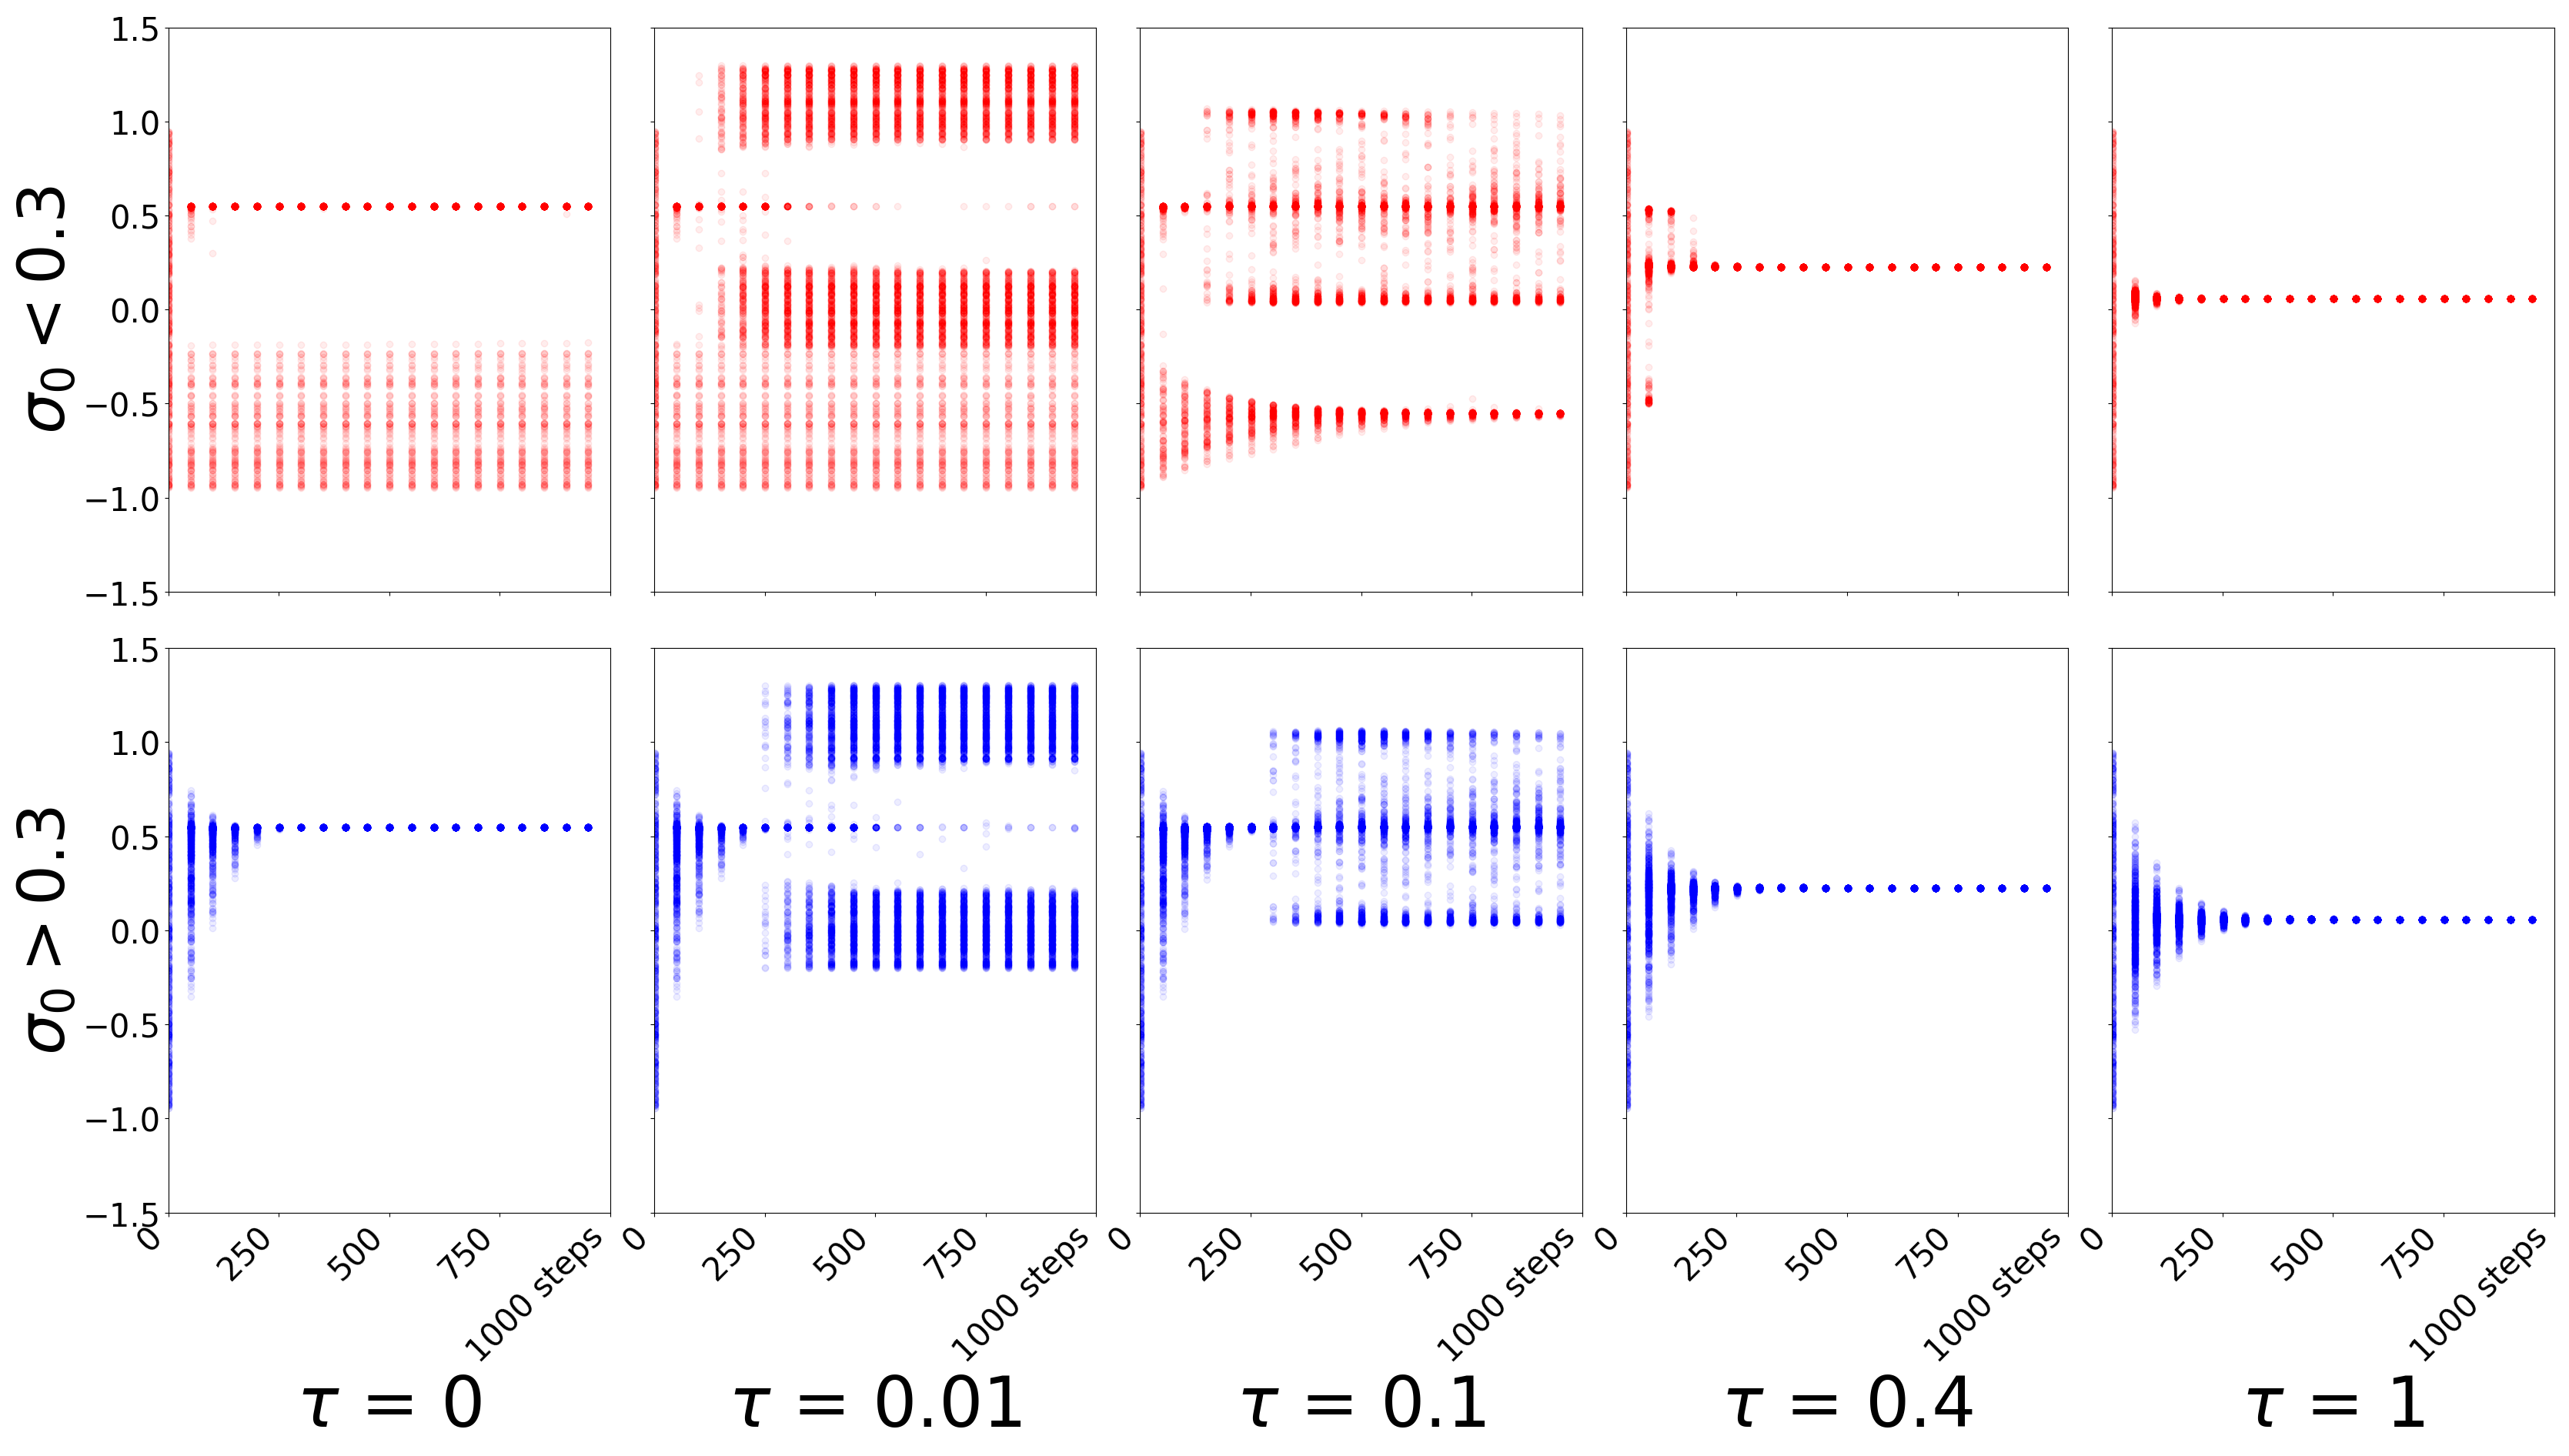
\includegraphics[width=1\columnwidth]{figs/bandit/notlearnQ/modes=1/sgd/mean_forward_optim=sgd_modes=1_lr=0.01.png}
%     \caption{Forward KL, SGD.}
%     \label{fig:bandit-mean-forward-sgd}
%   \end{subfigure}%
%   \begin{subfigure}[b]{0.4\linewidth}
%     \centering
%     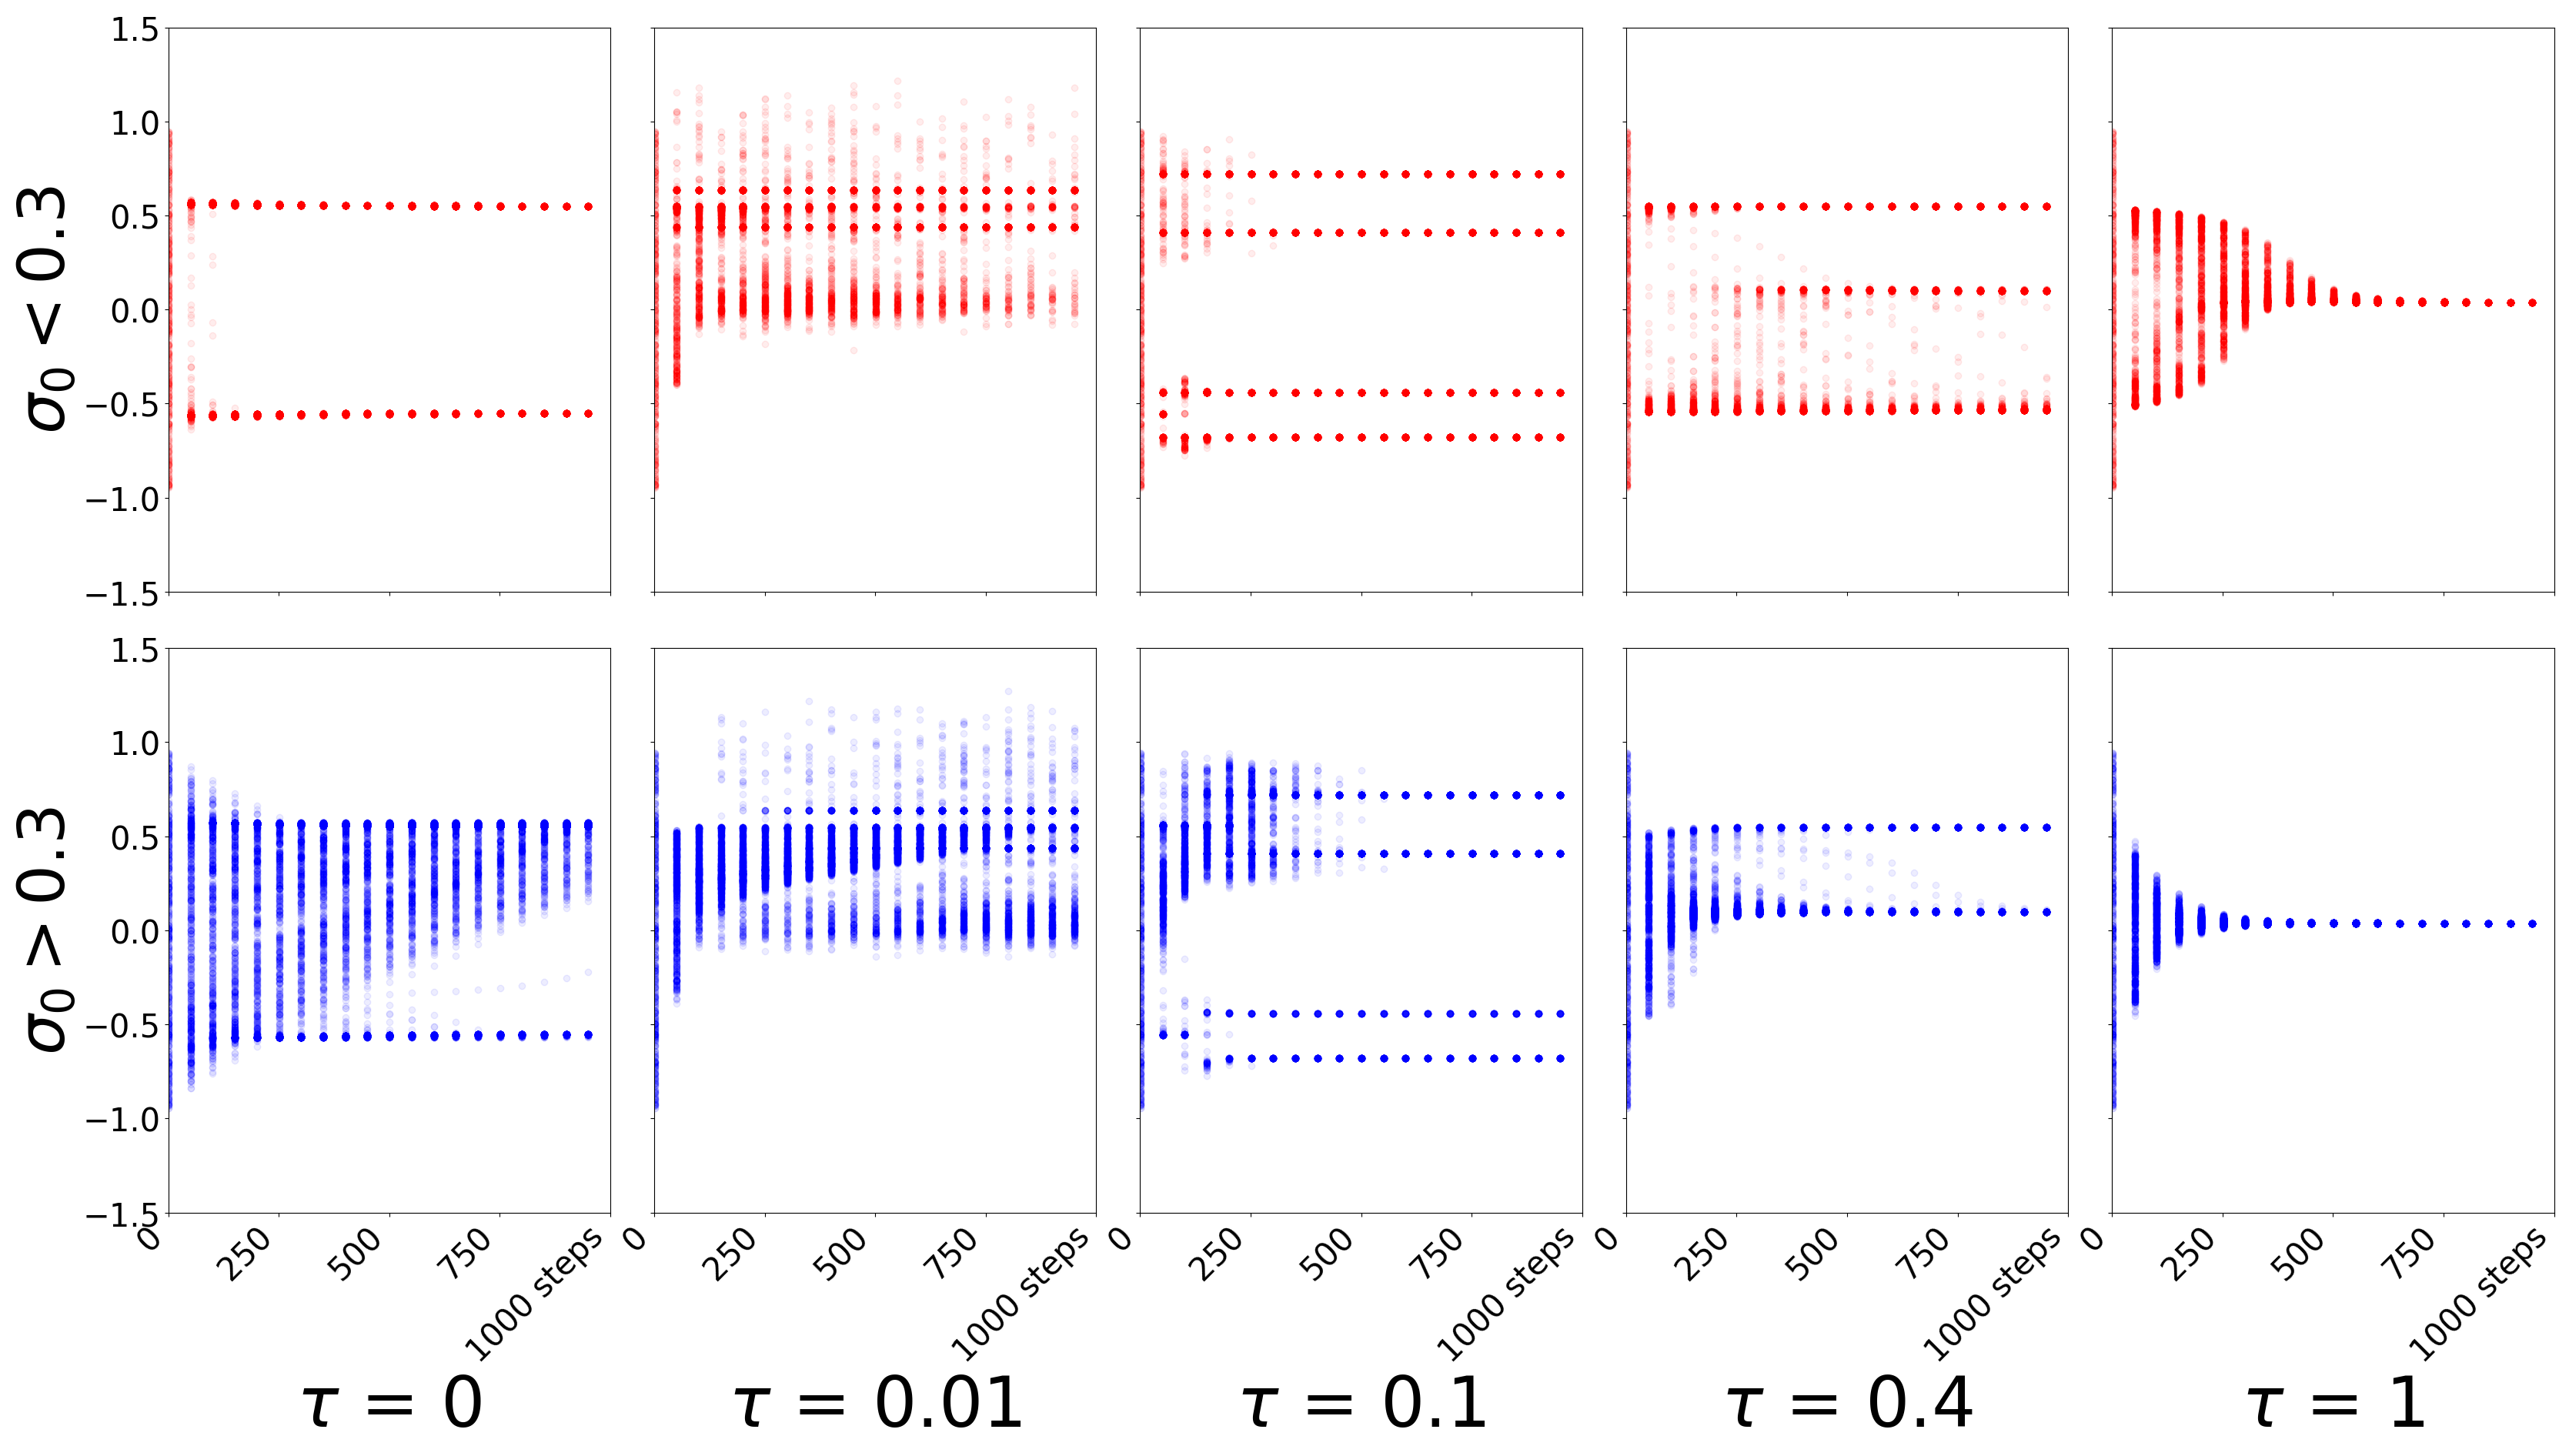
\includegraphics[width=1\columnwidth]{figs/bandit/notlearnQ/modes=1/sgd/mean_reverse_optim=sgd_modes=1_lr=0.01.png}
%     \caption{Reverse KL, SGD.}
%     \label{fig:bandit-mean-reverse-sgd}
%   \end{subfigure}
%   \caption{Mean over time with unimodal policy. }
% \end{figure}

% \begin{figure}[!ht]
%   \centering
%   \begin{subfigure}[b]{0.4\linewidth}
%     \centering
%     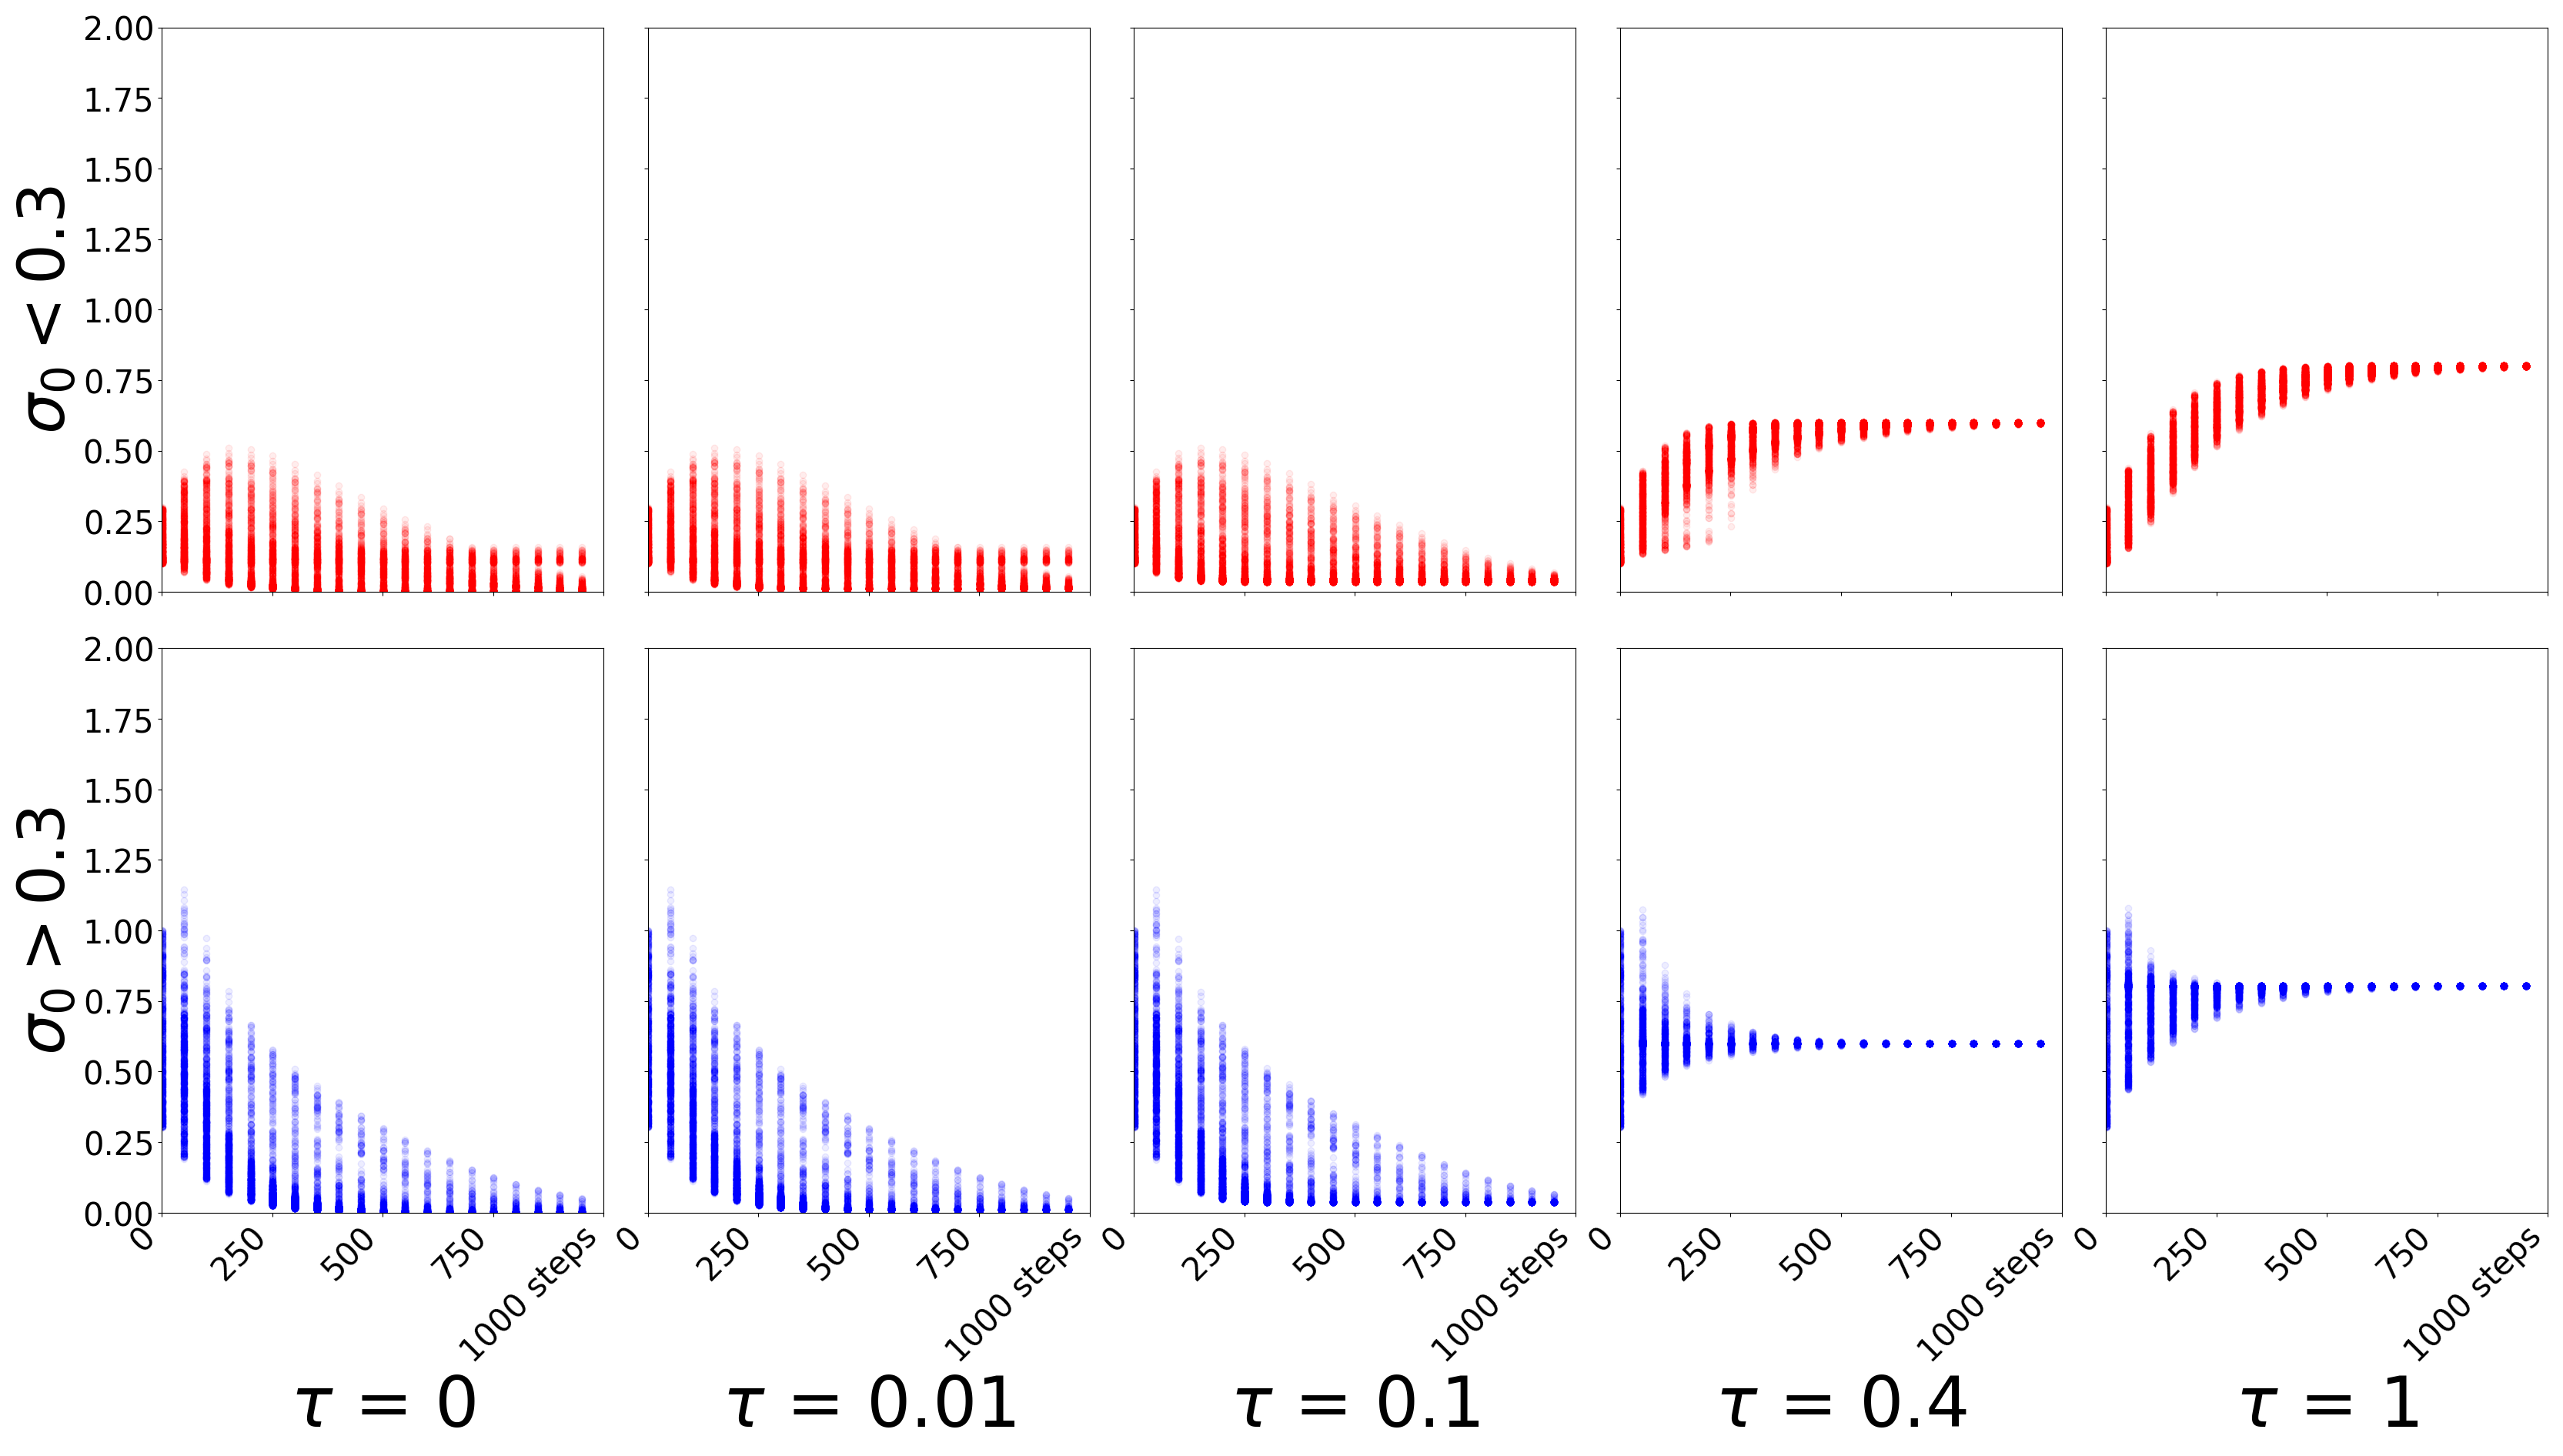
\includegraphics[width=1\columnwidth]{figs/bandit/notlearnQ/modes=1/adam/std_forward_optim=adam_modes=1_lr=0.01.png}
%     \caption{Forward KL, Adam.}
%     \label{fig:bandit-std-forward-adam}
%   \end{subfigure}%
%   \begin{subfigure}[b]{0.4\linewidth}
%     \centering
%     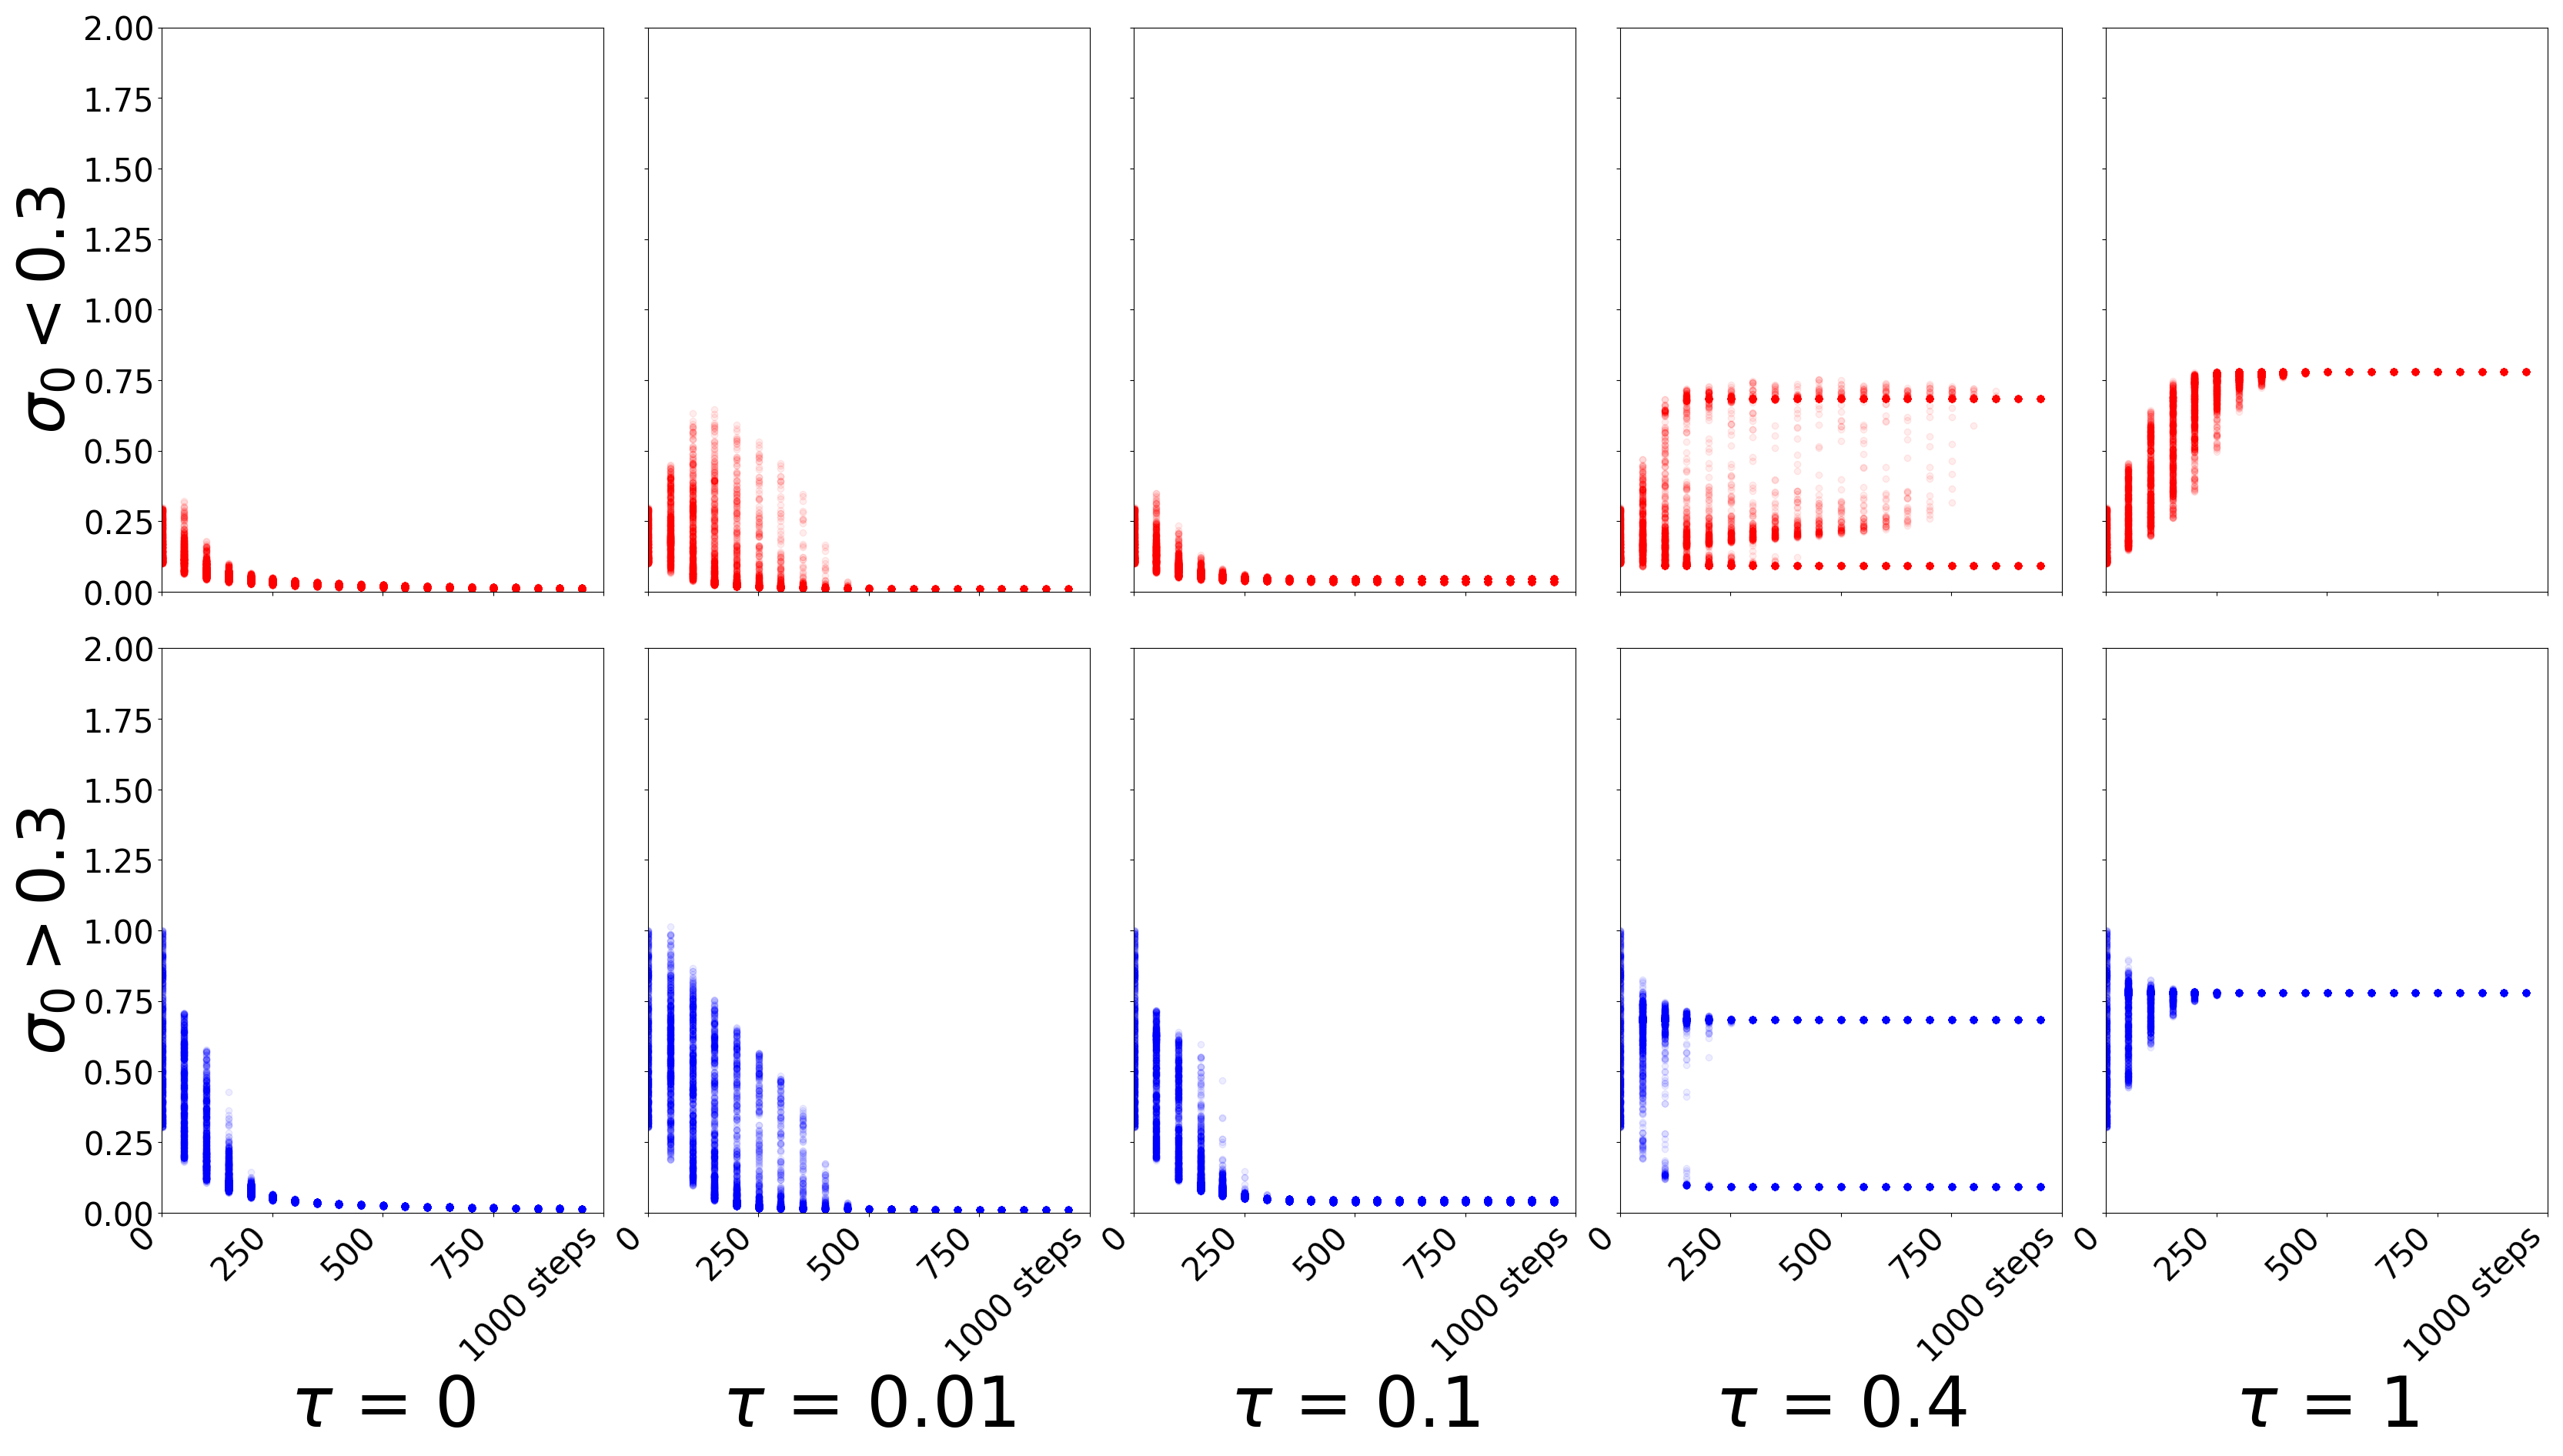
\includegraphics[width=1\columnwidth]{figs/bandit/notlearnQ/modes=1/adam/std_reverse_optim=adam_modes=1_lr=0.01.png}
%     \caption{Reverse KL, Adam. }
%     \label{fig:bandit-std-reverse-adam}
%   \end{subfigure}
  
%   \begin{subfigure}[b]{0.4\linewidth}
%     \centering
%     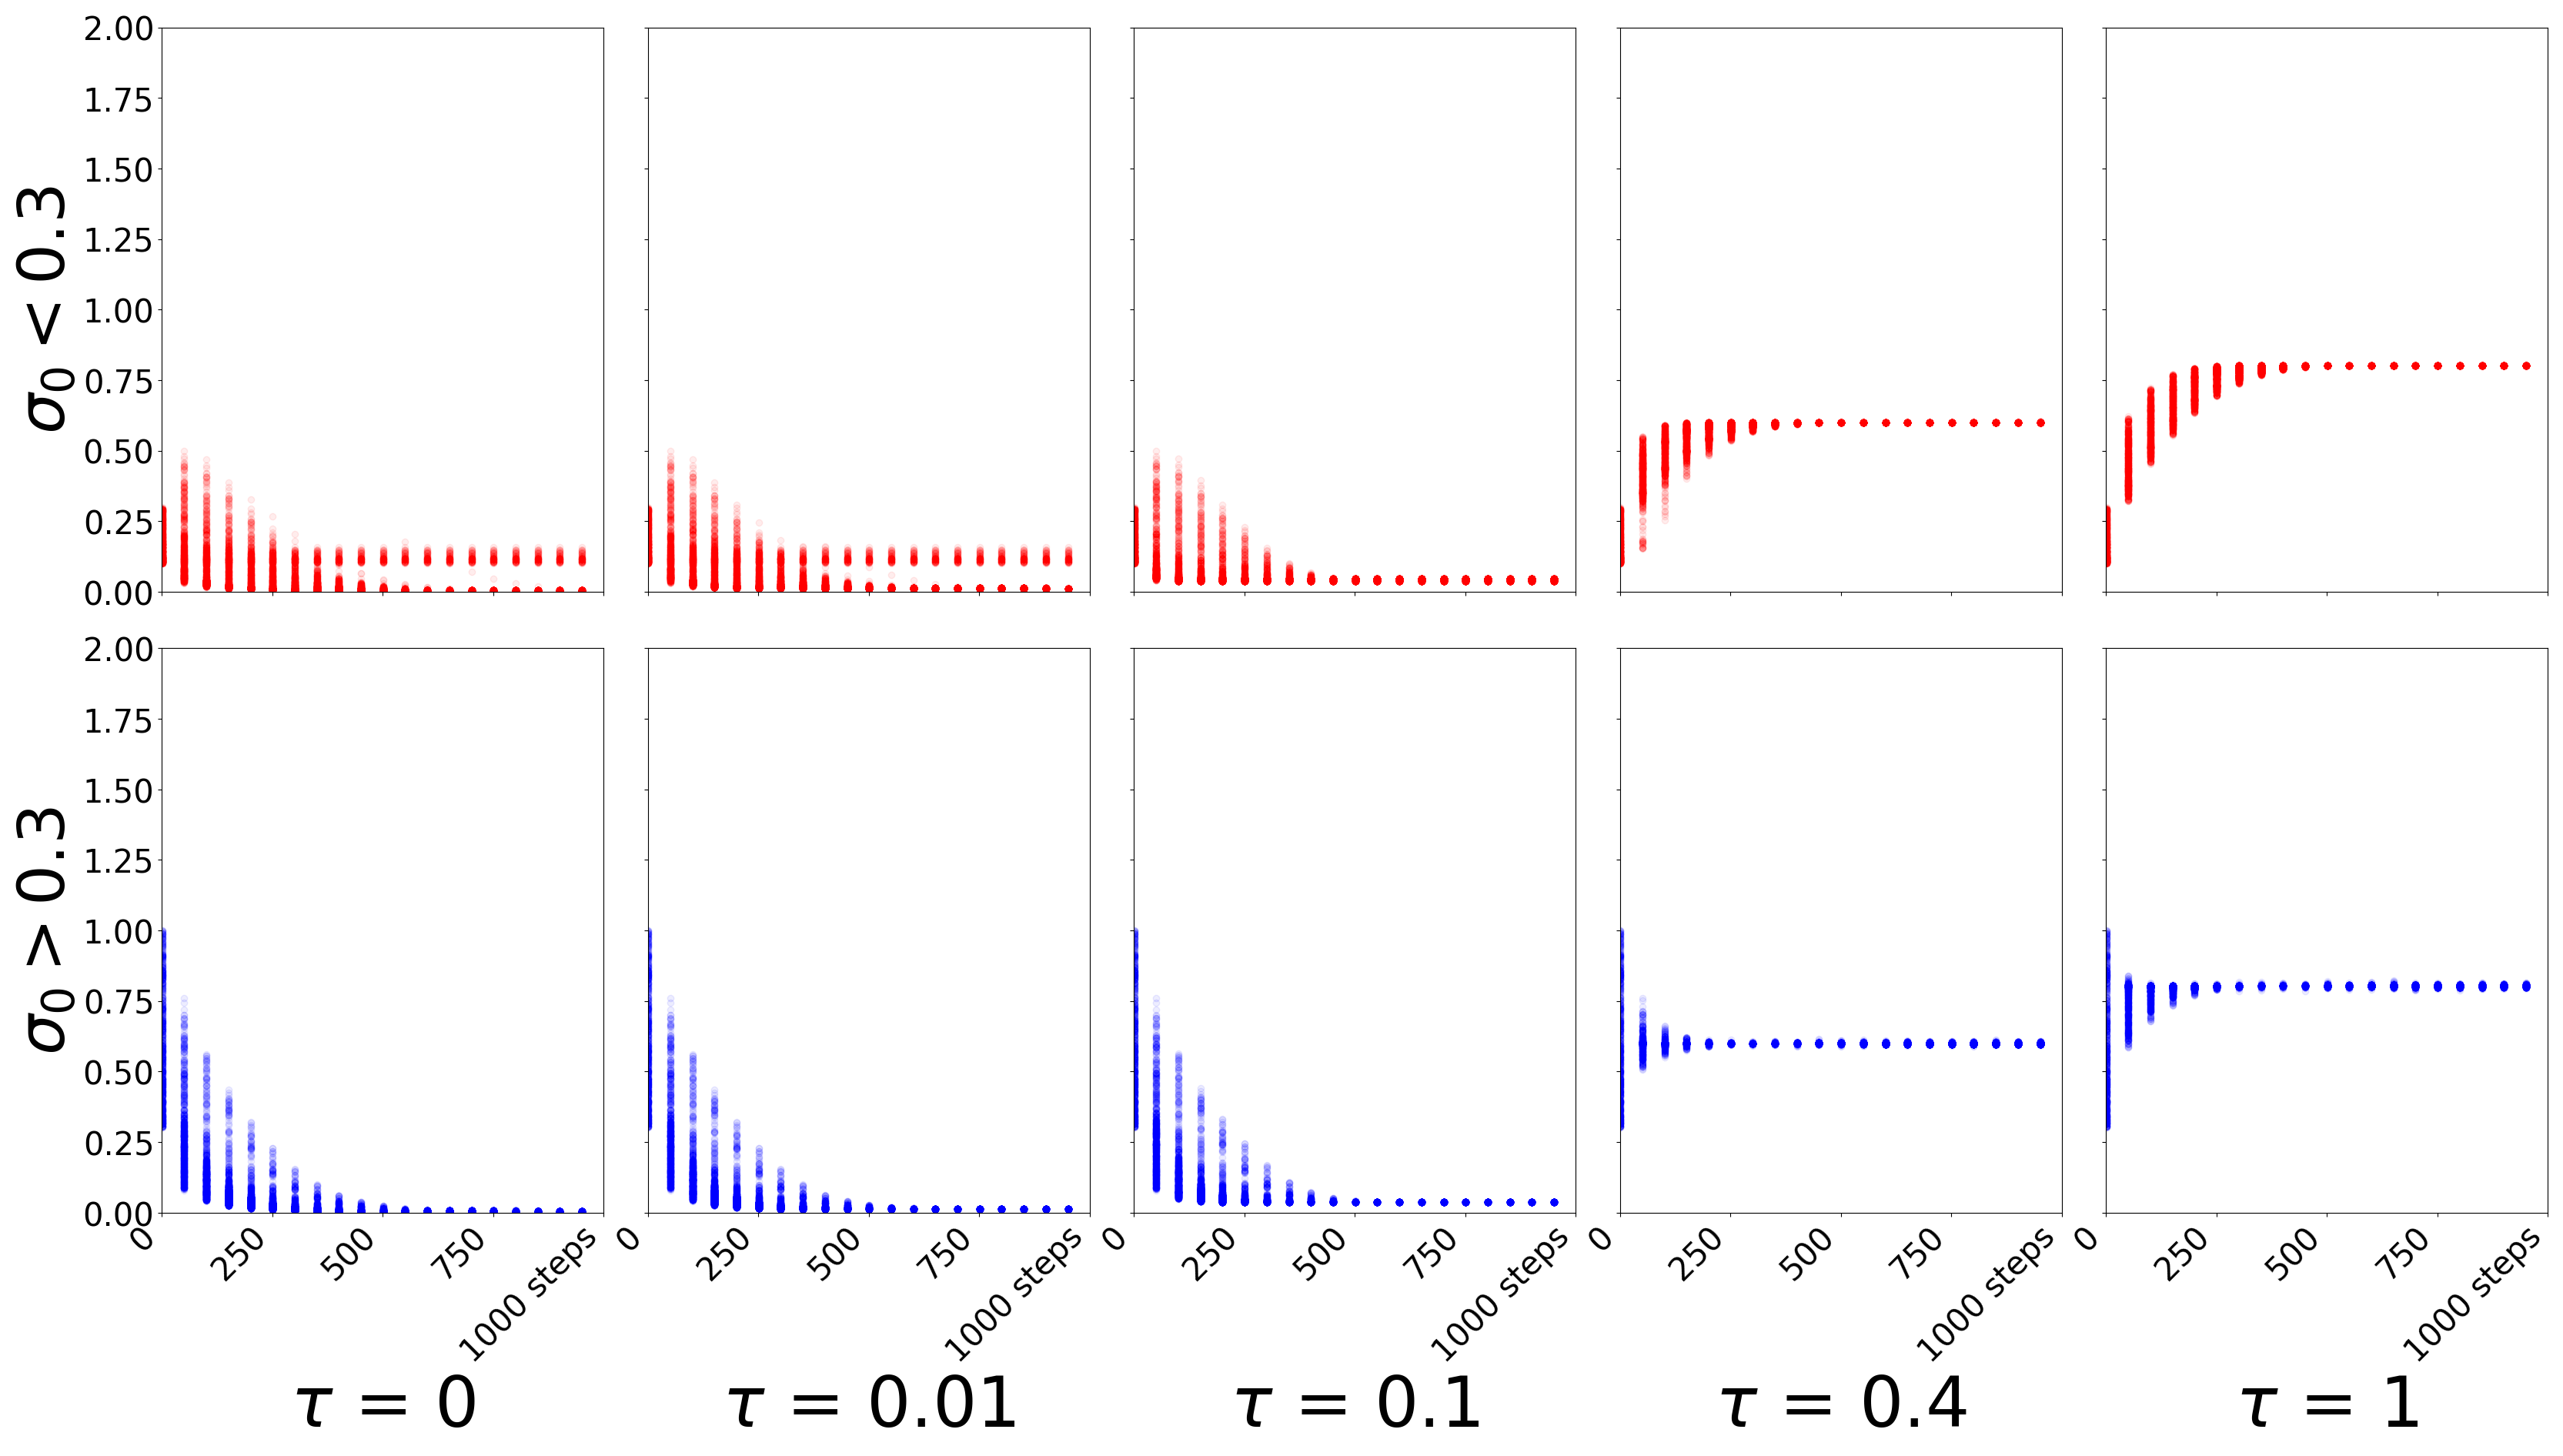
\includegraphics[width=1\columnwidth]{figs/bandit/notlearnQ/modes=1/rmsprop/std_forward_optim=rmsprop_modes=1_lr=0.01.png}
%     \caption{Forward KL, RMSprop.}
%     \label{fig:bandit-std-forward-rmsprop}
%   \end{subfigure}%
%   \begin{subfigure}[b]{0.4\linewidth}
%     \centering
%     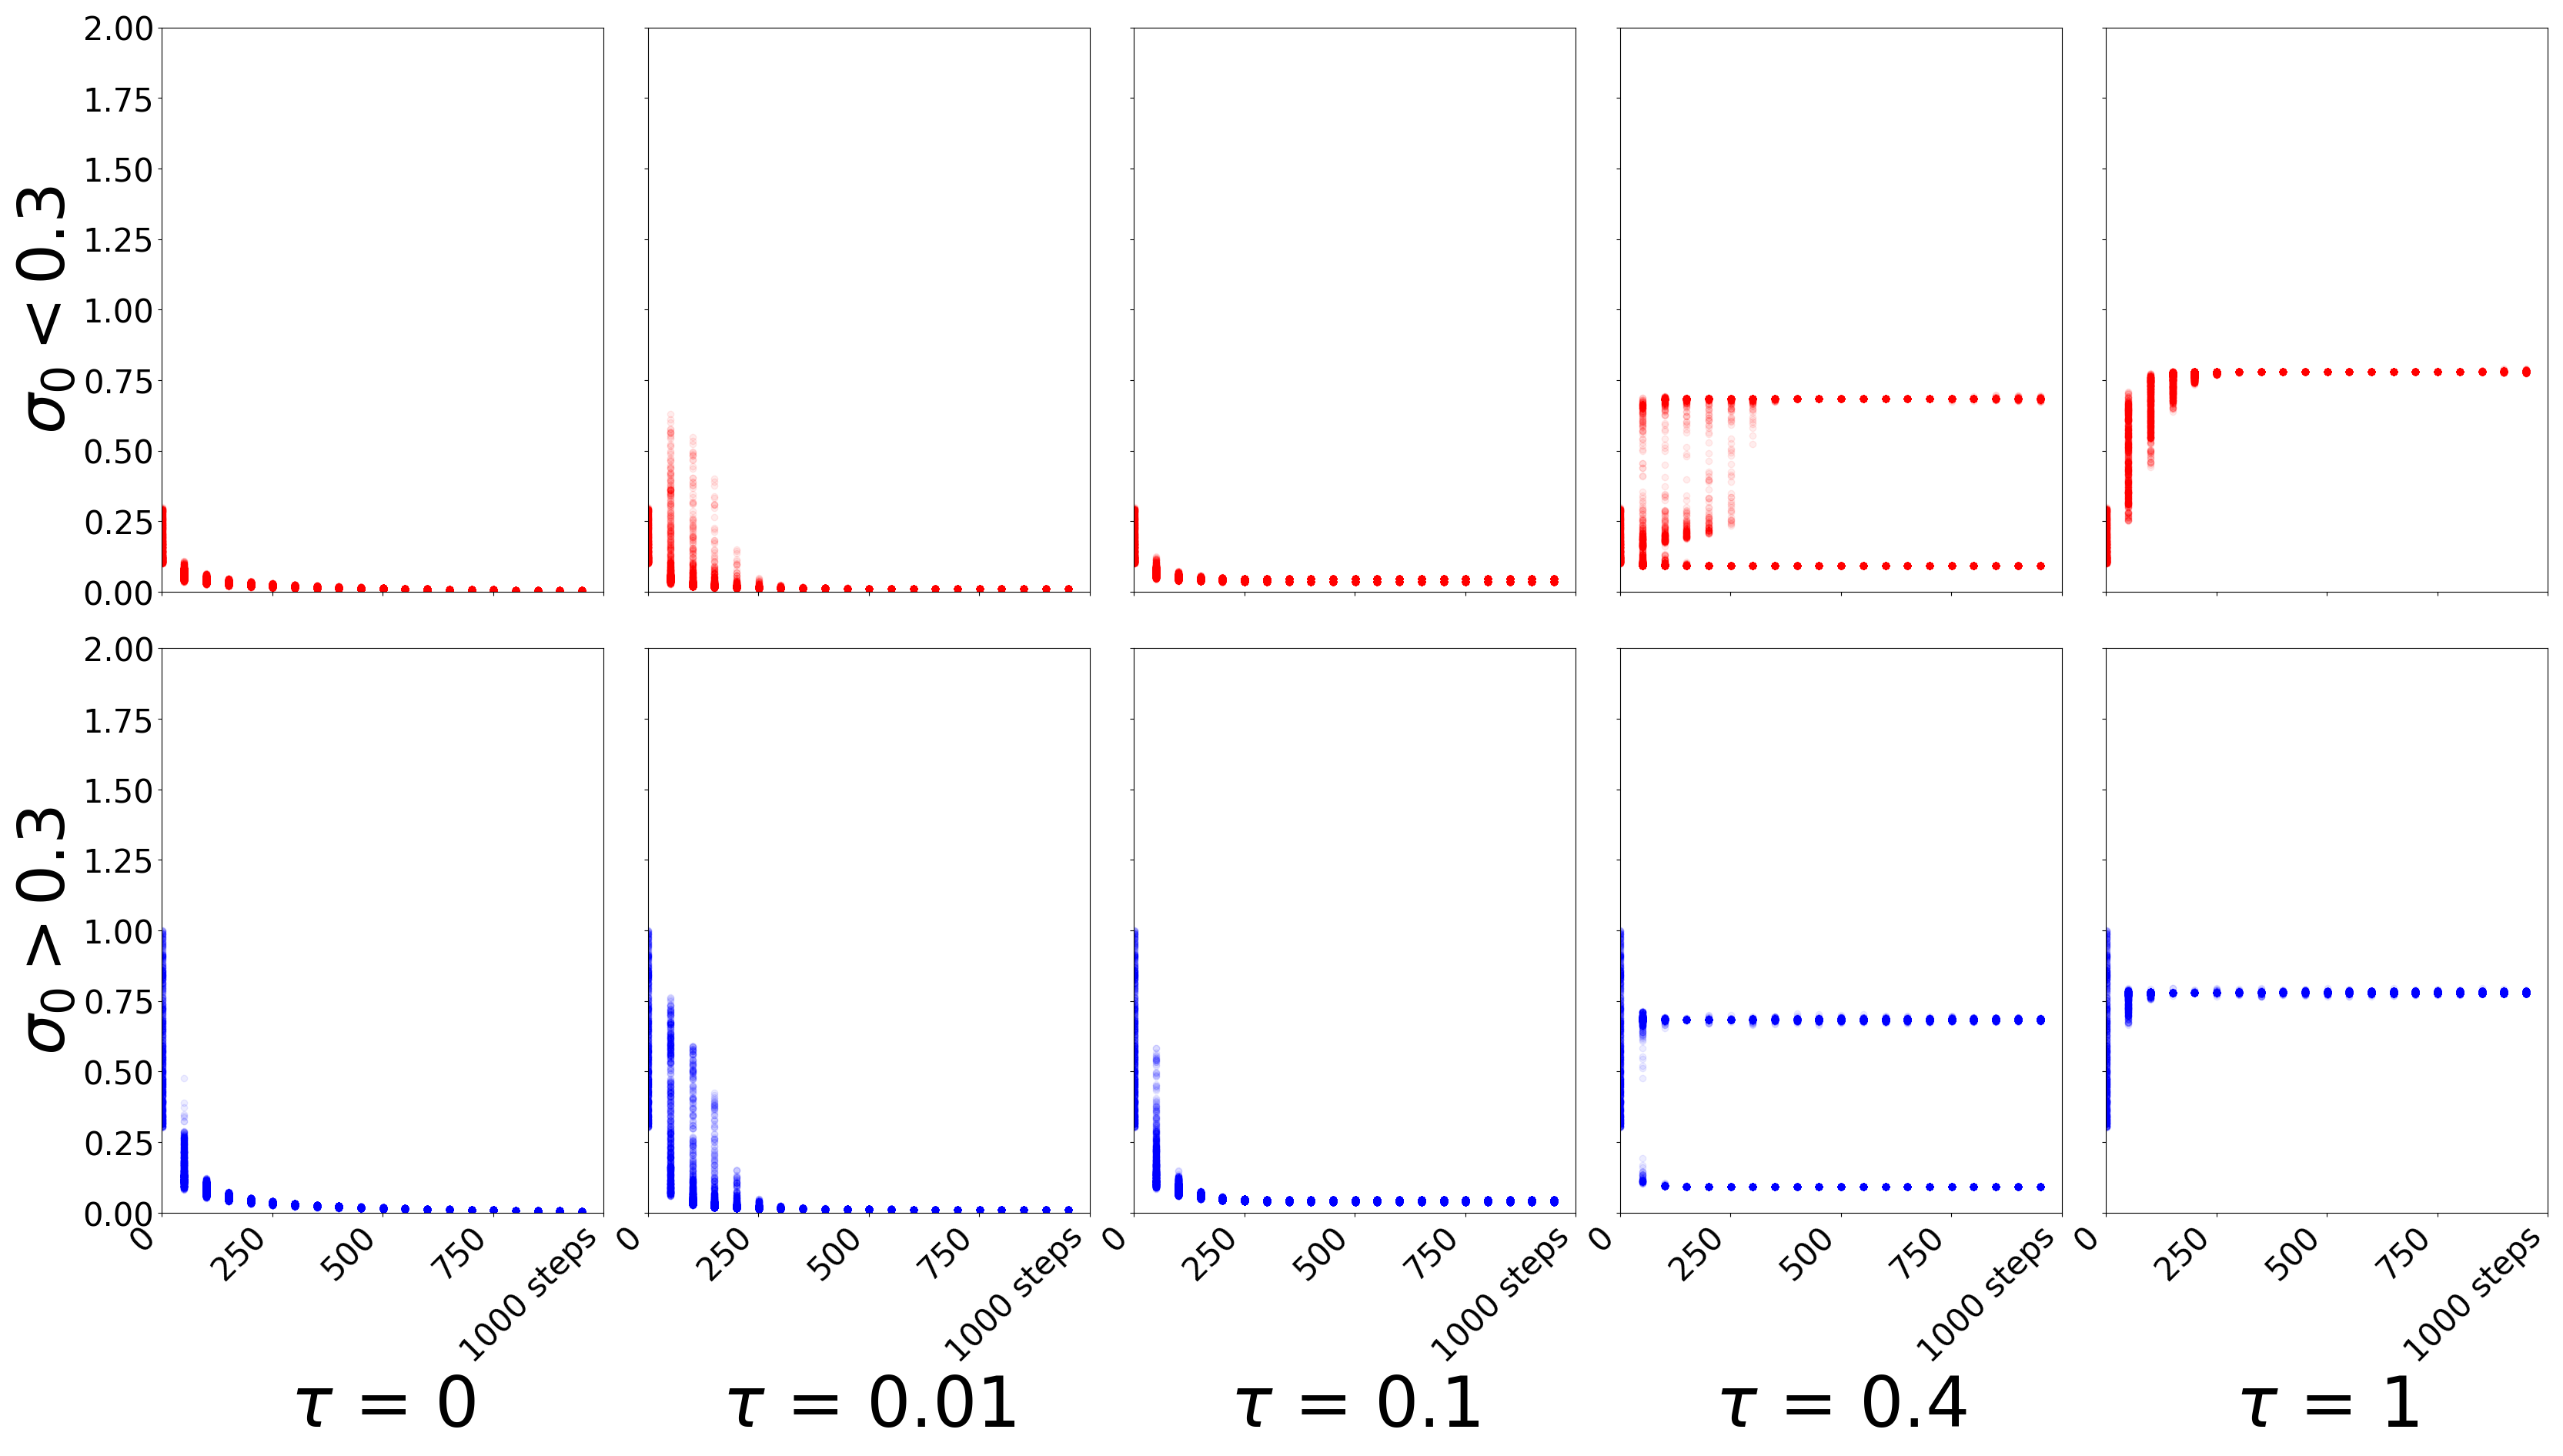
\includegraphics[width=1\columnwidth]{figs/bandit/notlearnQ/modes=1/rmsprop/std_reverse_optim=rmsprop_modes=1_lr=0.01.png}
%     \caption{Reverse KL, RMSprop.}
%     \label{fig:bandit-std-reverse-rmsprop}
%   \end{subfigure}
  
%   \begin{subfigure}[b]{0.4\linewidth}
%     \centering
%     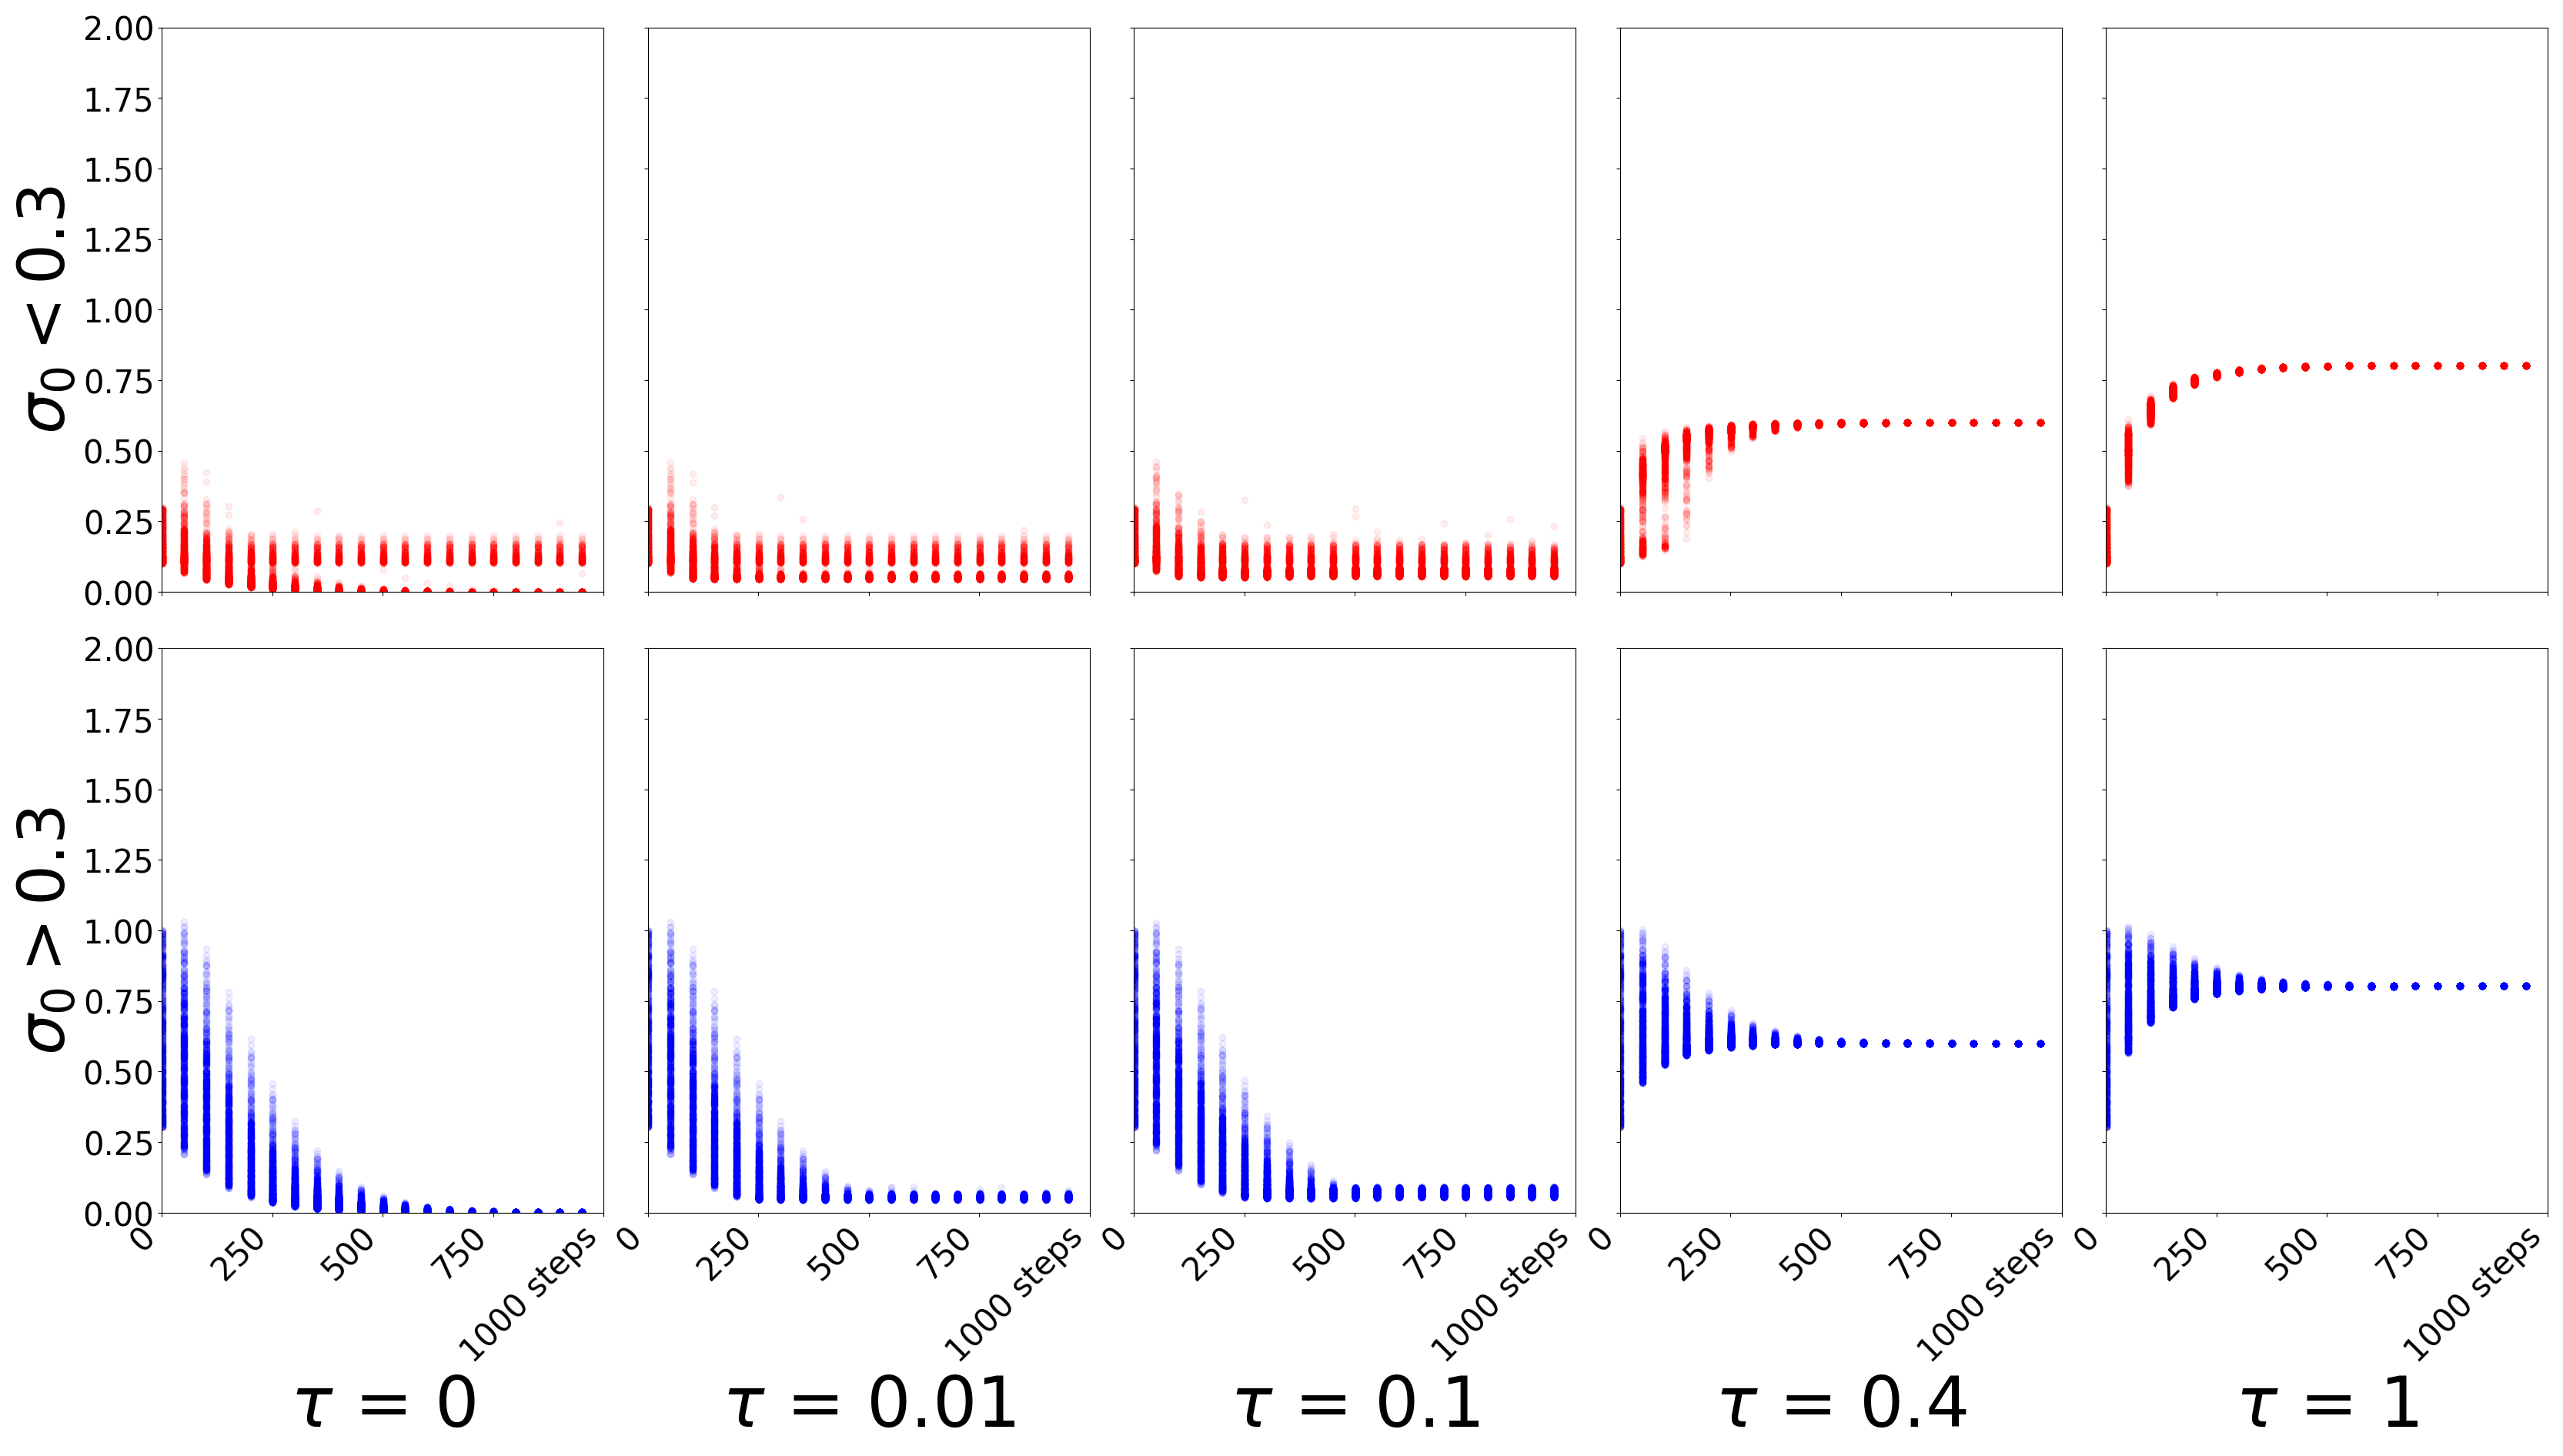
\includegraphics[width=1\columnwidth]{figs/bandit/notlearnQ/modes=1/sgd/std_forward_optim=sgd_modes=1_lr=0.01.png}
%     \caption{Forward KL, SGD.}
%     \label{fig:bandit-std-forward-sgd}
%   \end{subfigure}%
%   \begin{subfigure}[b]{0.4\linewidth}
%     \centering
%     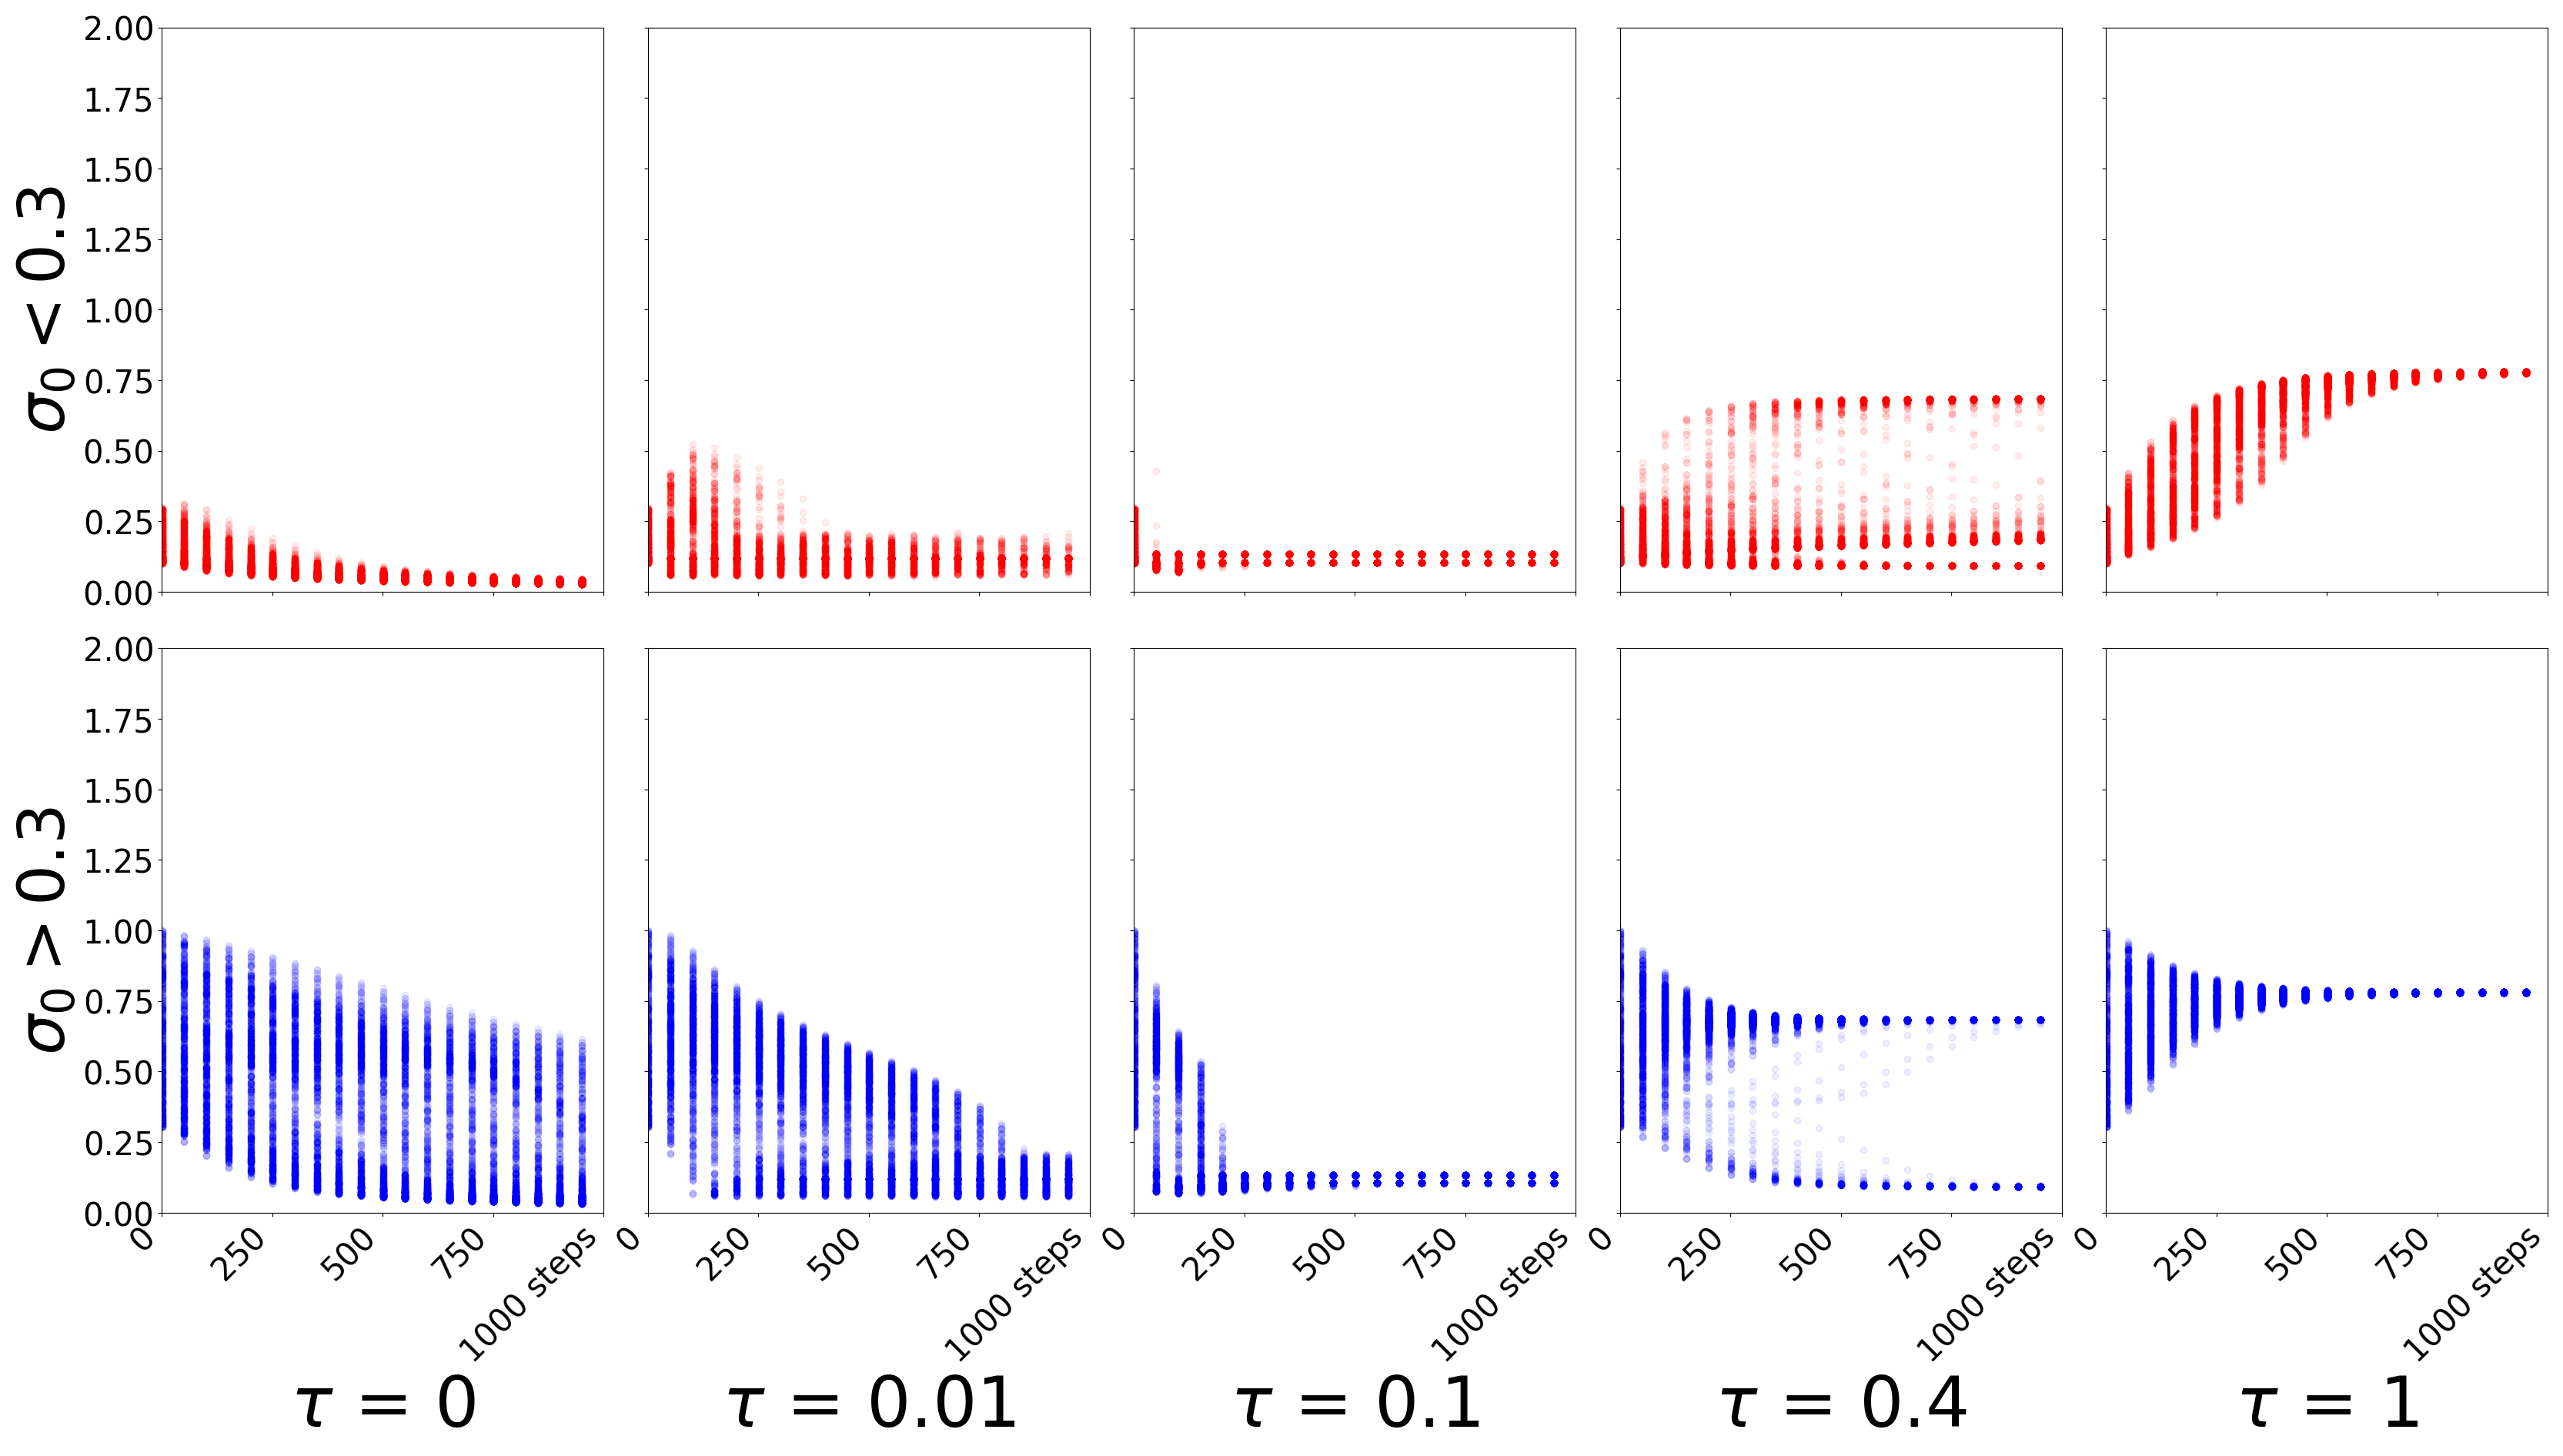
\includegraphics[width=1\columnwidth]{figs/bandit/notlearnQ/modes=1/sgd/std_reverse_optim=sgd_modes=1_lr=0.01.png}
%     \caption{Reverse KL, SGD.}
%     \label{fig:bandit-std-reverse-sgd}
%   \end{subfigure}
%   \caption{Standard deviation over time with unimodal policy. }
% \end{figure}


% \begin{figure}[!ht]
%   \centering
%   \begin{subfigure}[b]{0.4\linewidth}
%     \centering
%     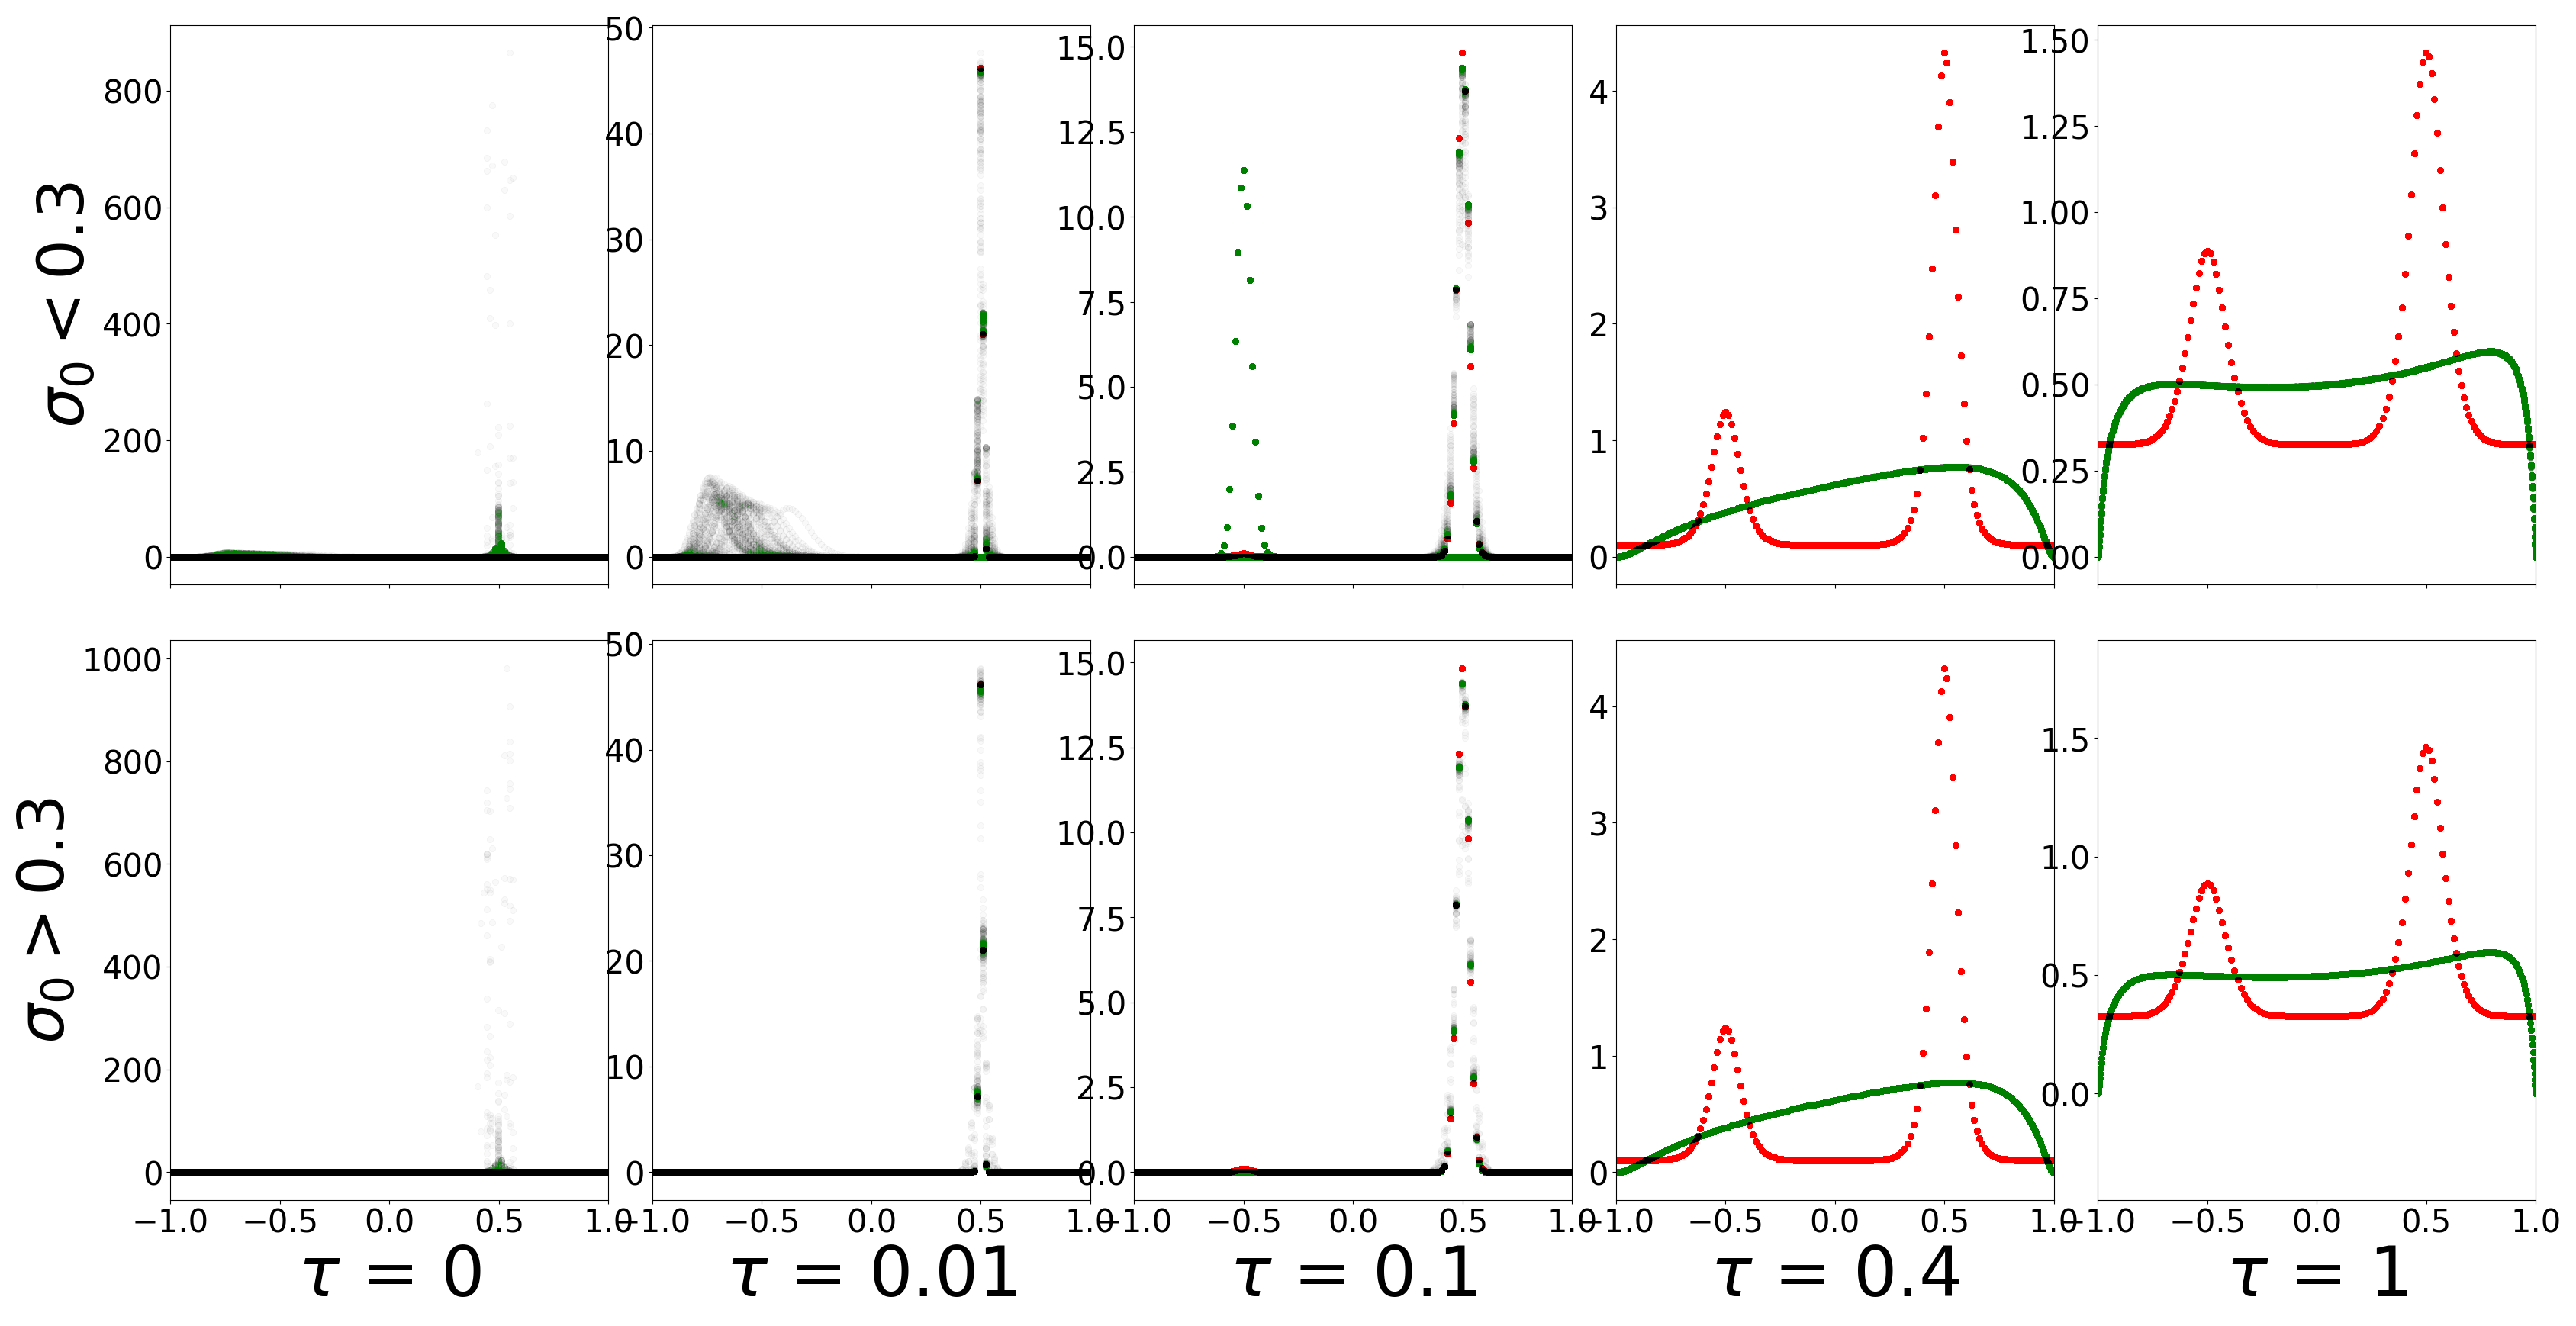
\includegraphics[width=1\columnwidth]{figs/bandit/notlearnQ/modes=1/adam/pdf_forward_optim=adam_modes=1_lr=0.01.png}
%     \caption{Forward KL, Adam.}
%     \label{fig:bandit-pdf-forward-adam}
%   \end{subfigure}%
%   \begin{subfigure}[b]{0.4\linewidth}
%     \centering
%     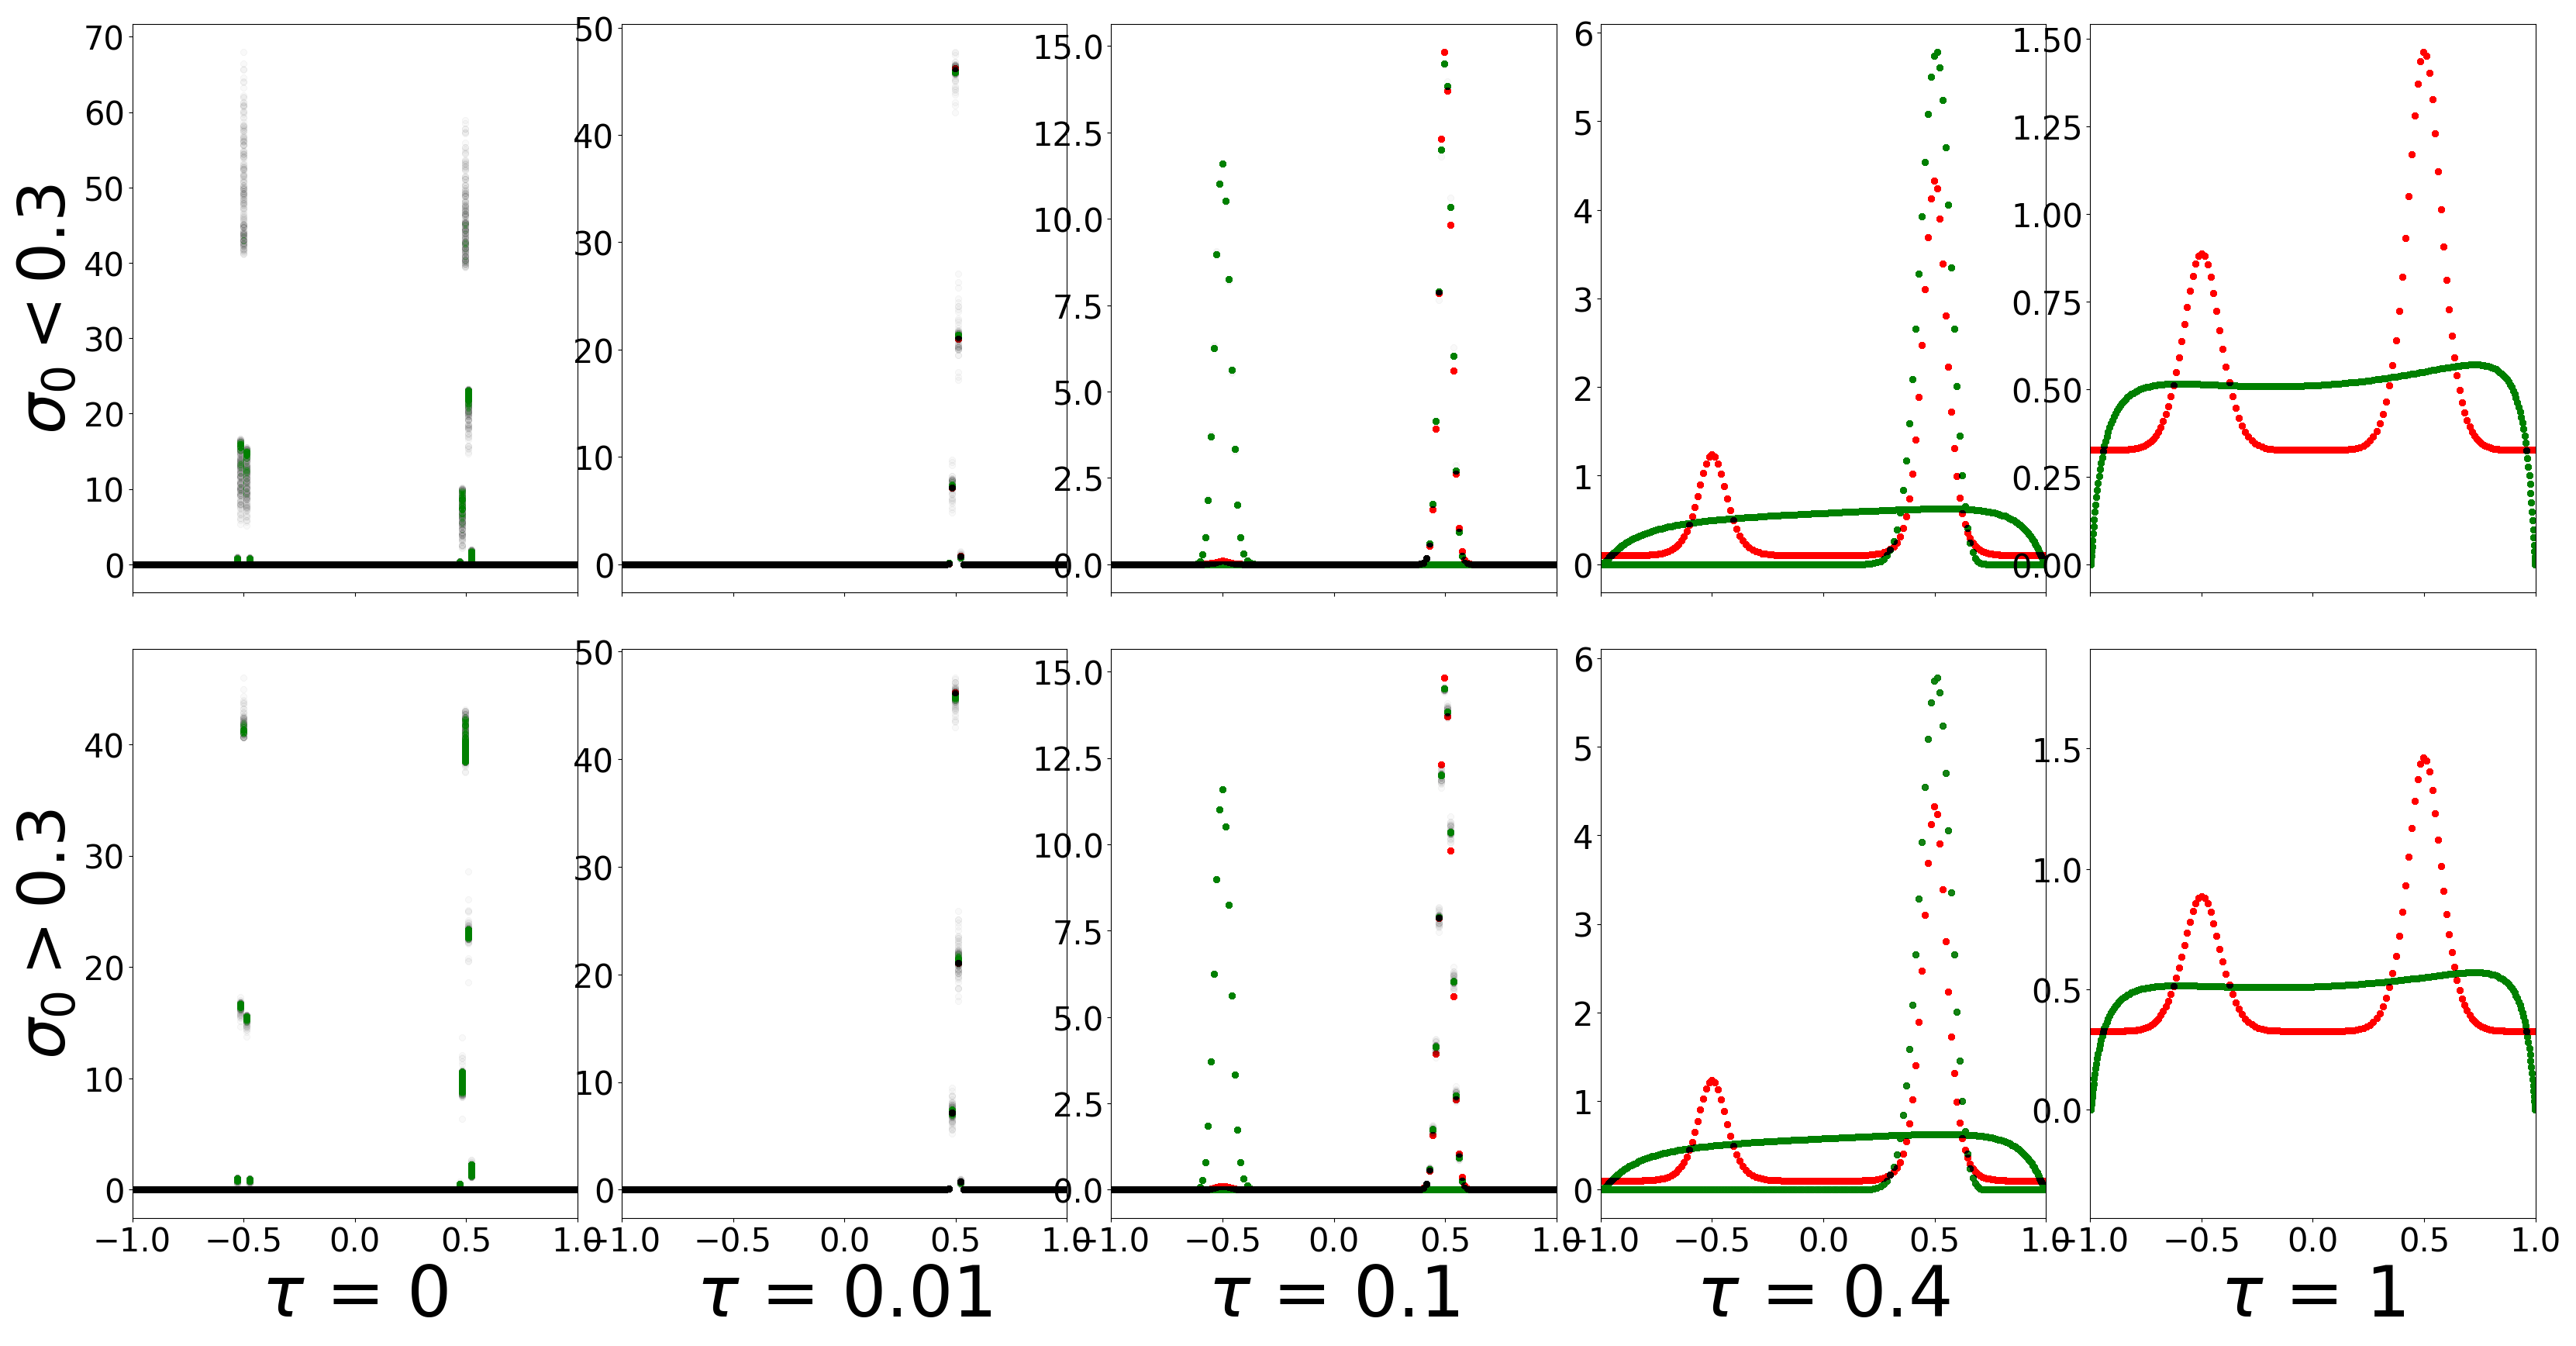
\includegraphics[width=1\columnwidth]{figs/bandit/notlearnQ/modes=1/adam/pdf_reverse_optim=adam_modes=1_lr=0.01.png}
%     \caption{Reverse KL, Adam. }
%     \label{fig:bandit-pdf-reverse-adam}
%   \end{subfigure}
  
%   \begin{subfigure}[b]{0.4\linewidth}
%     \centering
%     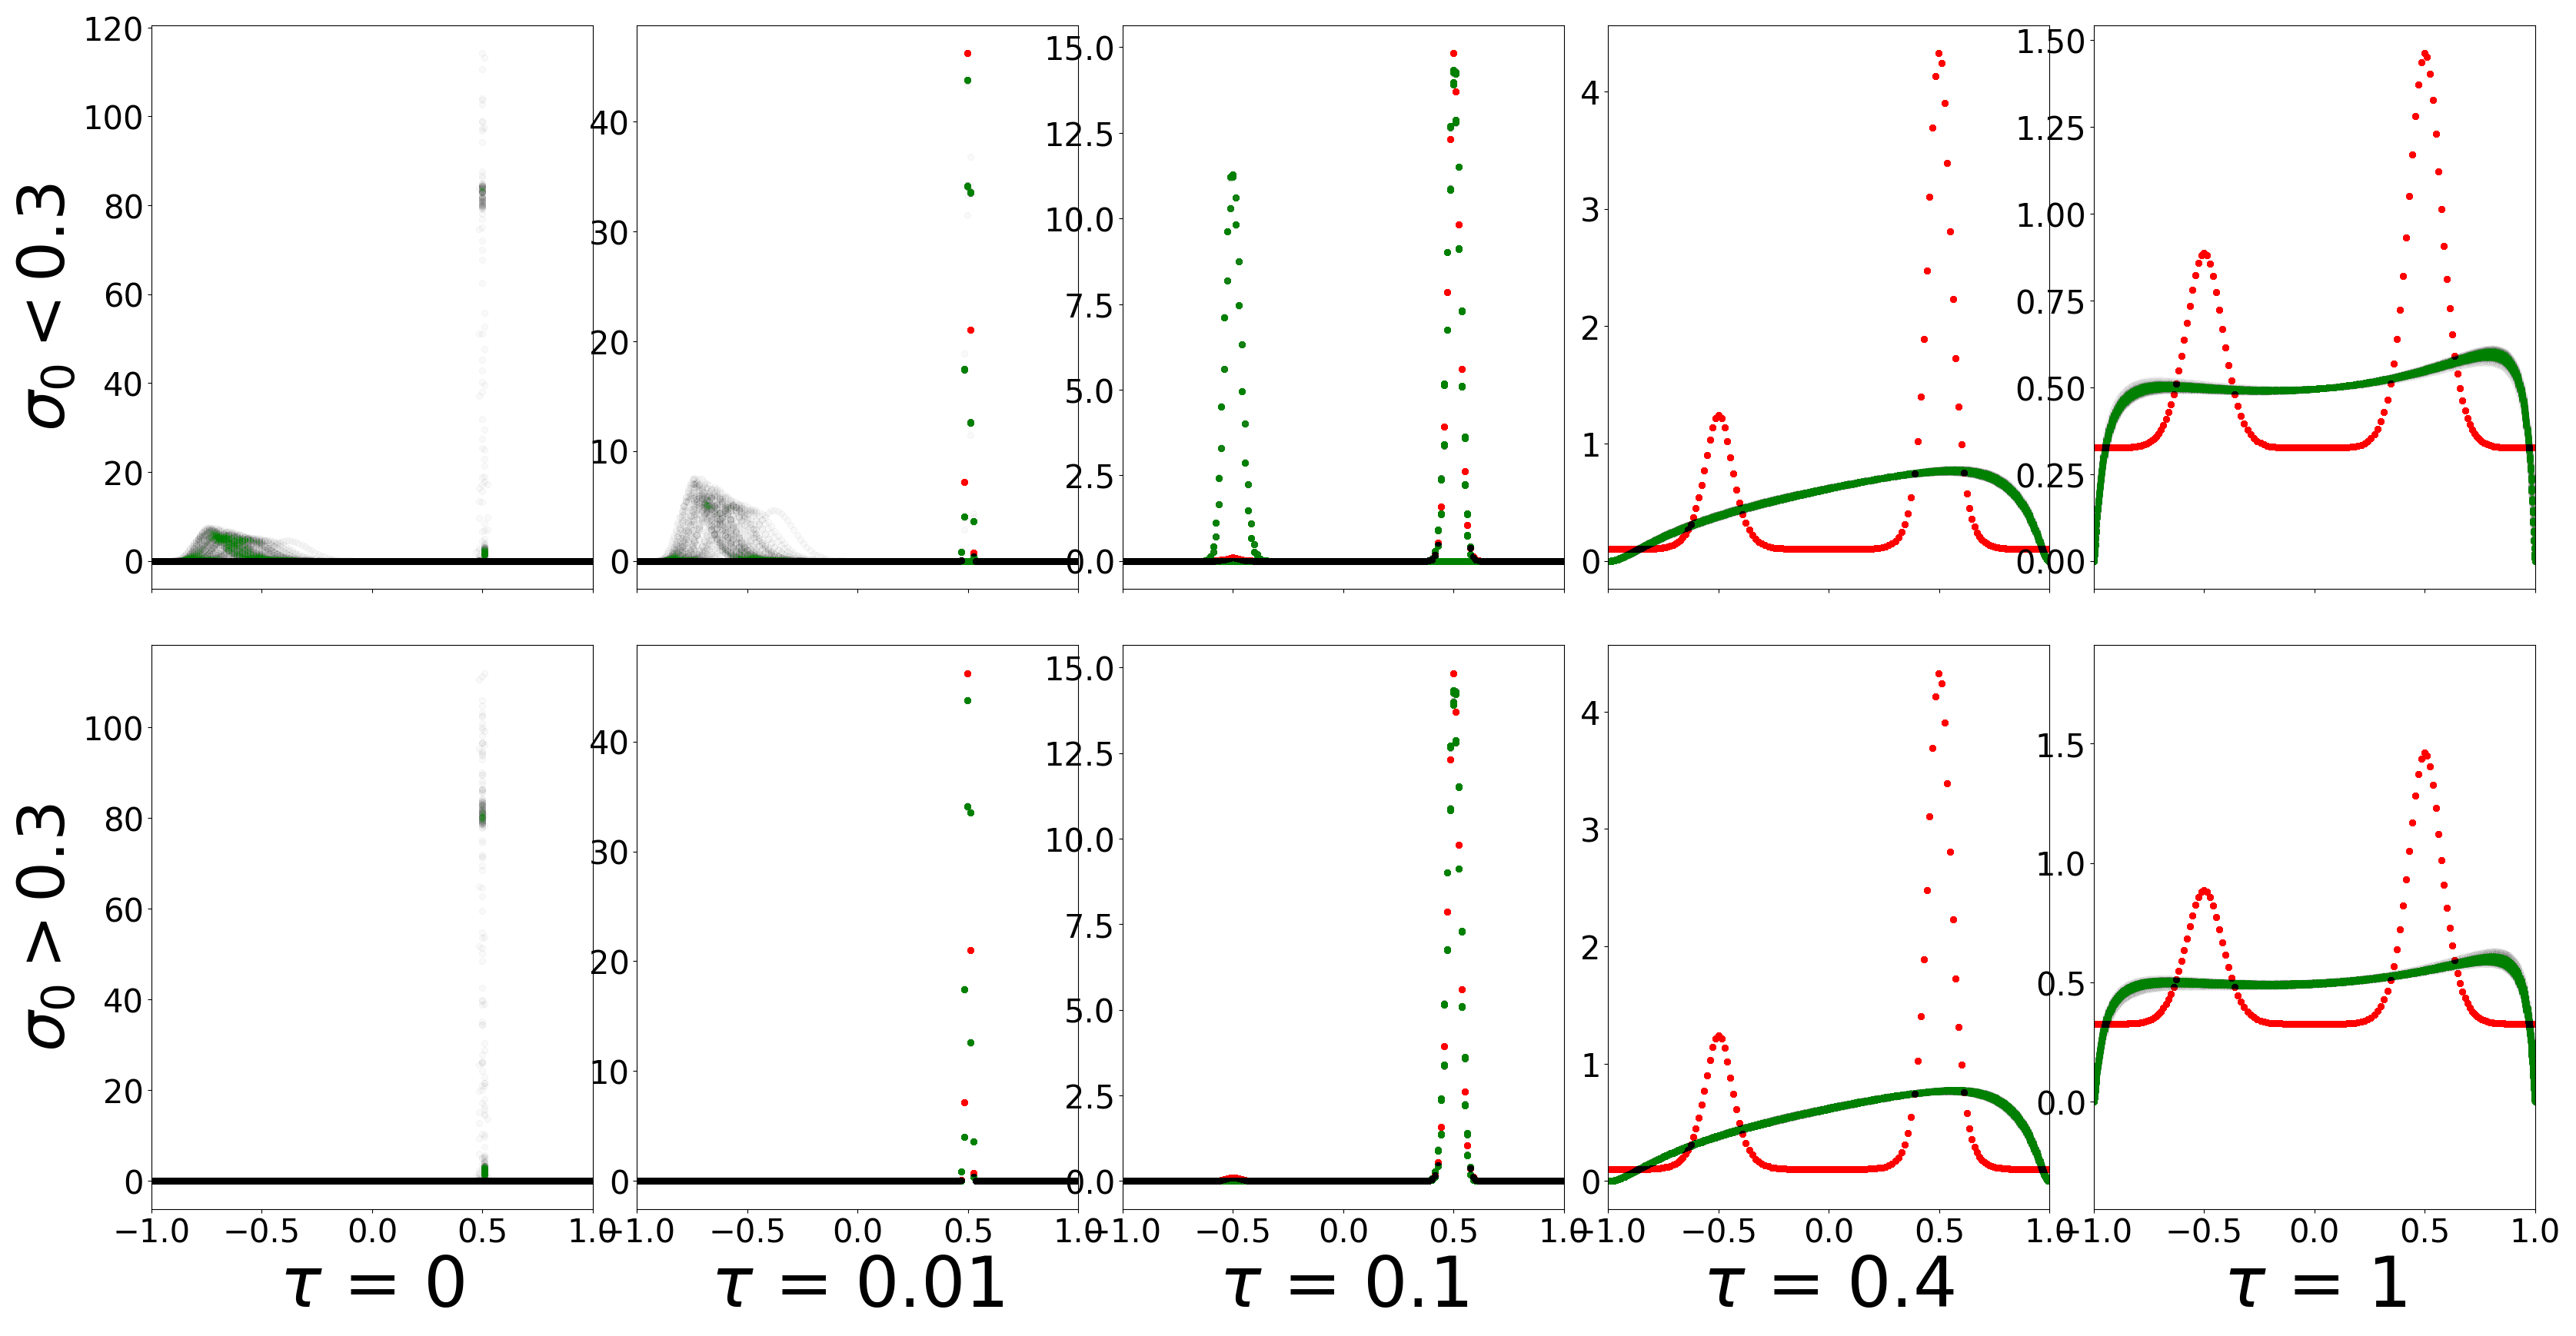
\includegraphics[width=1\columnwidth]{figs/bandit/notlearnQ/modes=1/rmsprop/pdf_forward_optim=rmsprop_modes=1_lr=0.01.png}
%     \caption{Forward KL, RMSprop.}
%     \label{fig:bandit-pdf-forward-rmsprop}
%   \end{subfigure}%
%   \begin{subfigure}[b]{0.4\linewidth}
%     \centering
%     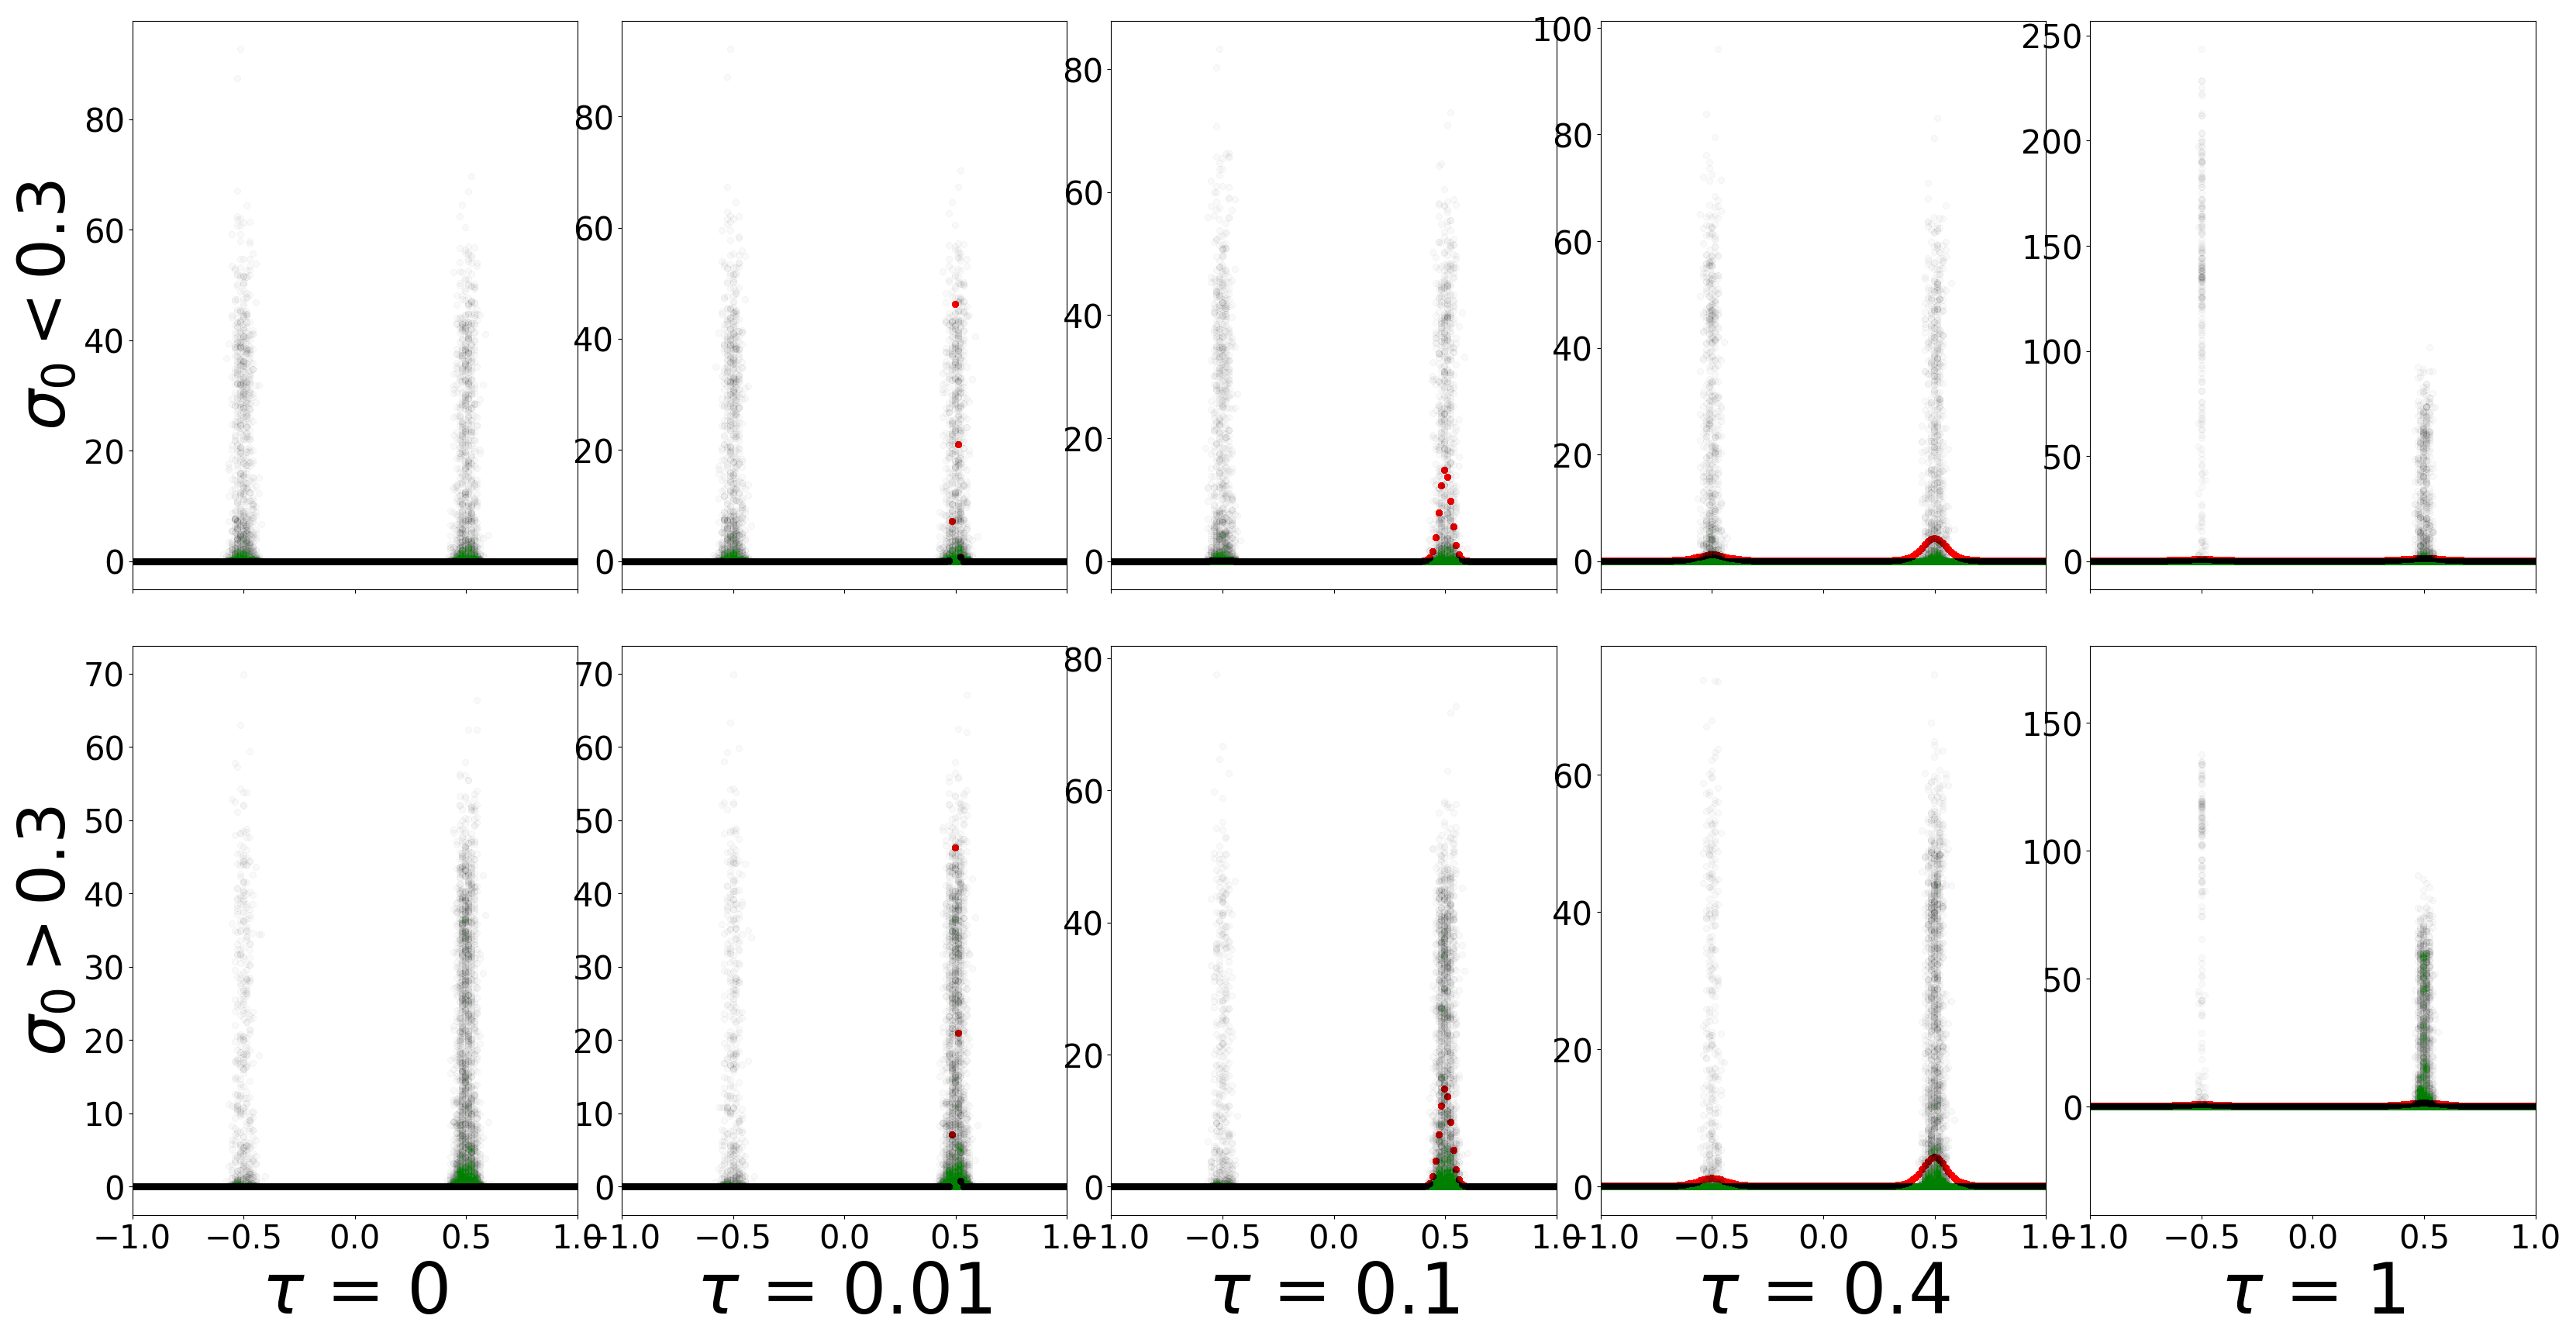
\includegraphics[width=1\columnwidth]{figs/bandit/notlearnQ/modes=1/rmsprop/pdf_reverse_optim=rmsprop_modes=1_lr=0.01.png}
%     \caption{Reverse KL, RMSprop.}
%     \label{fig:bandit-pdf-reverse-rmsprop}
%   \end{subfigure}
  
%   \begin{subfigure}[b]{0.4\linewidth}
%     \centering
%     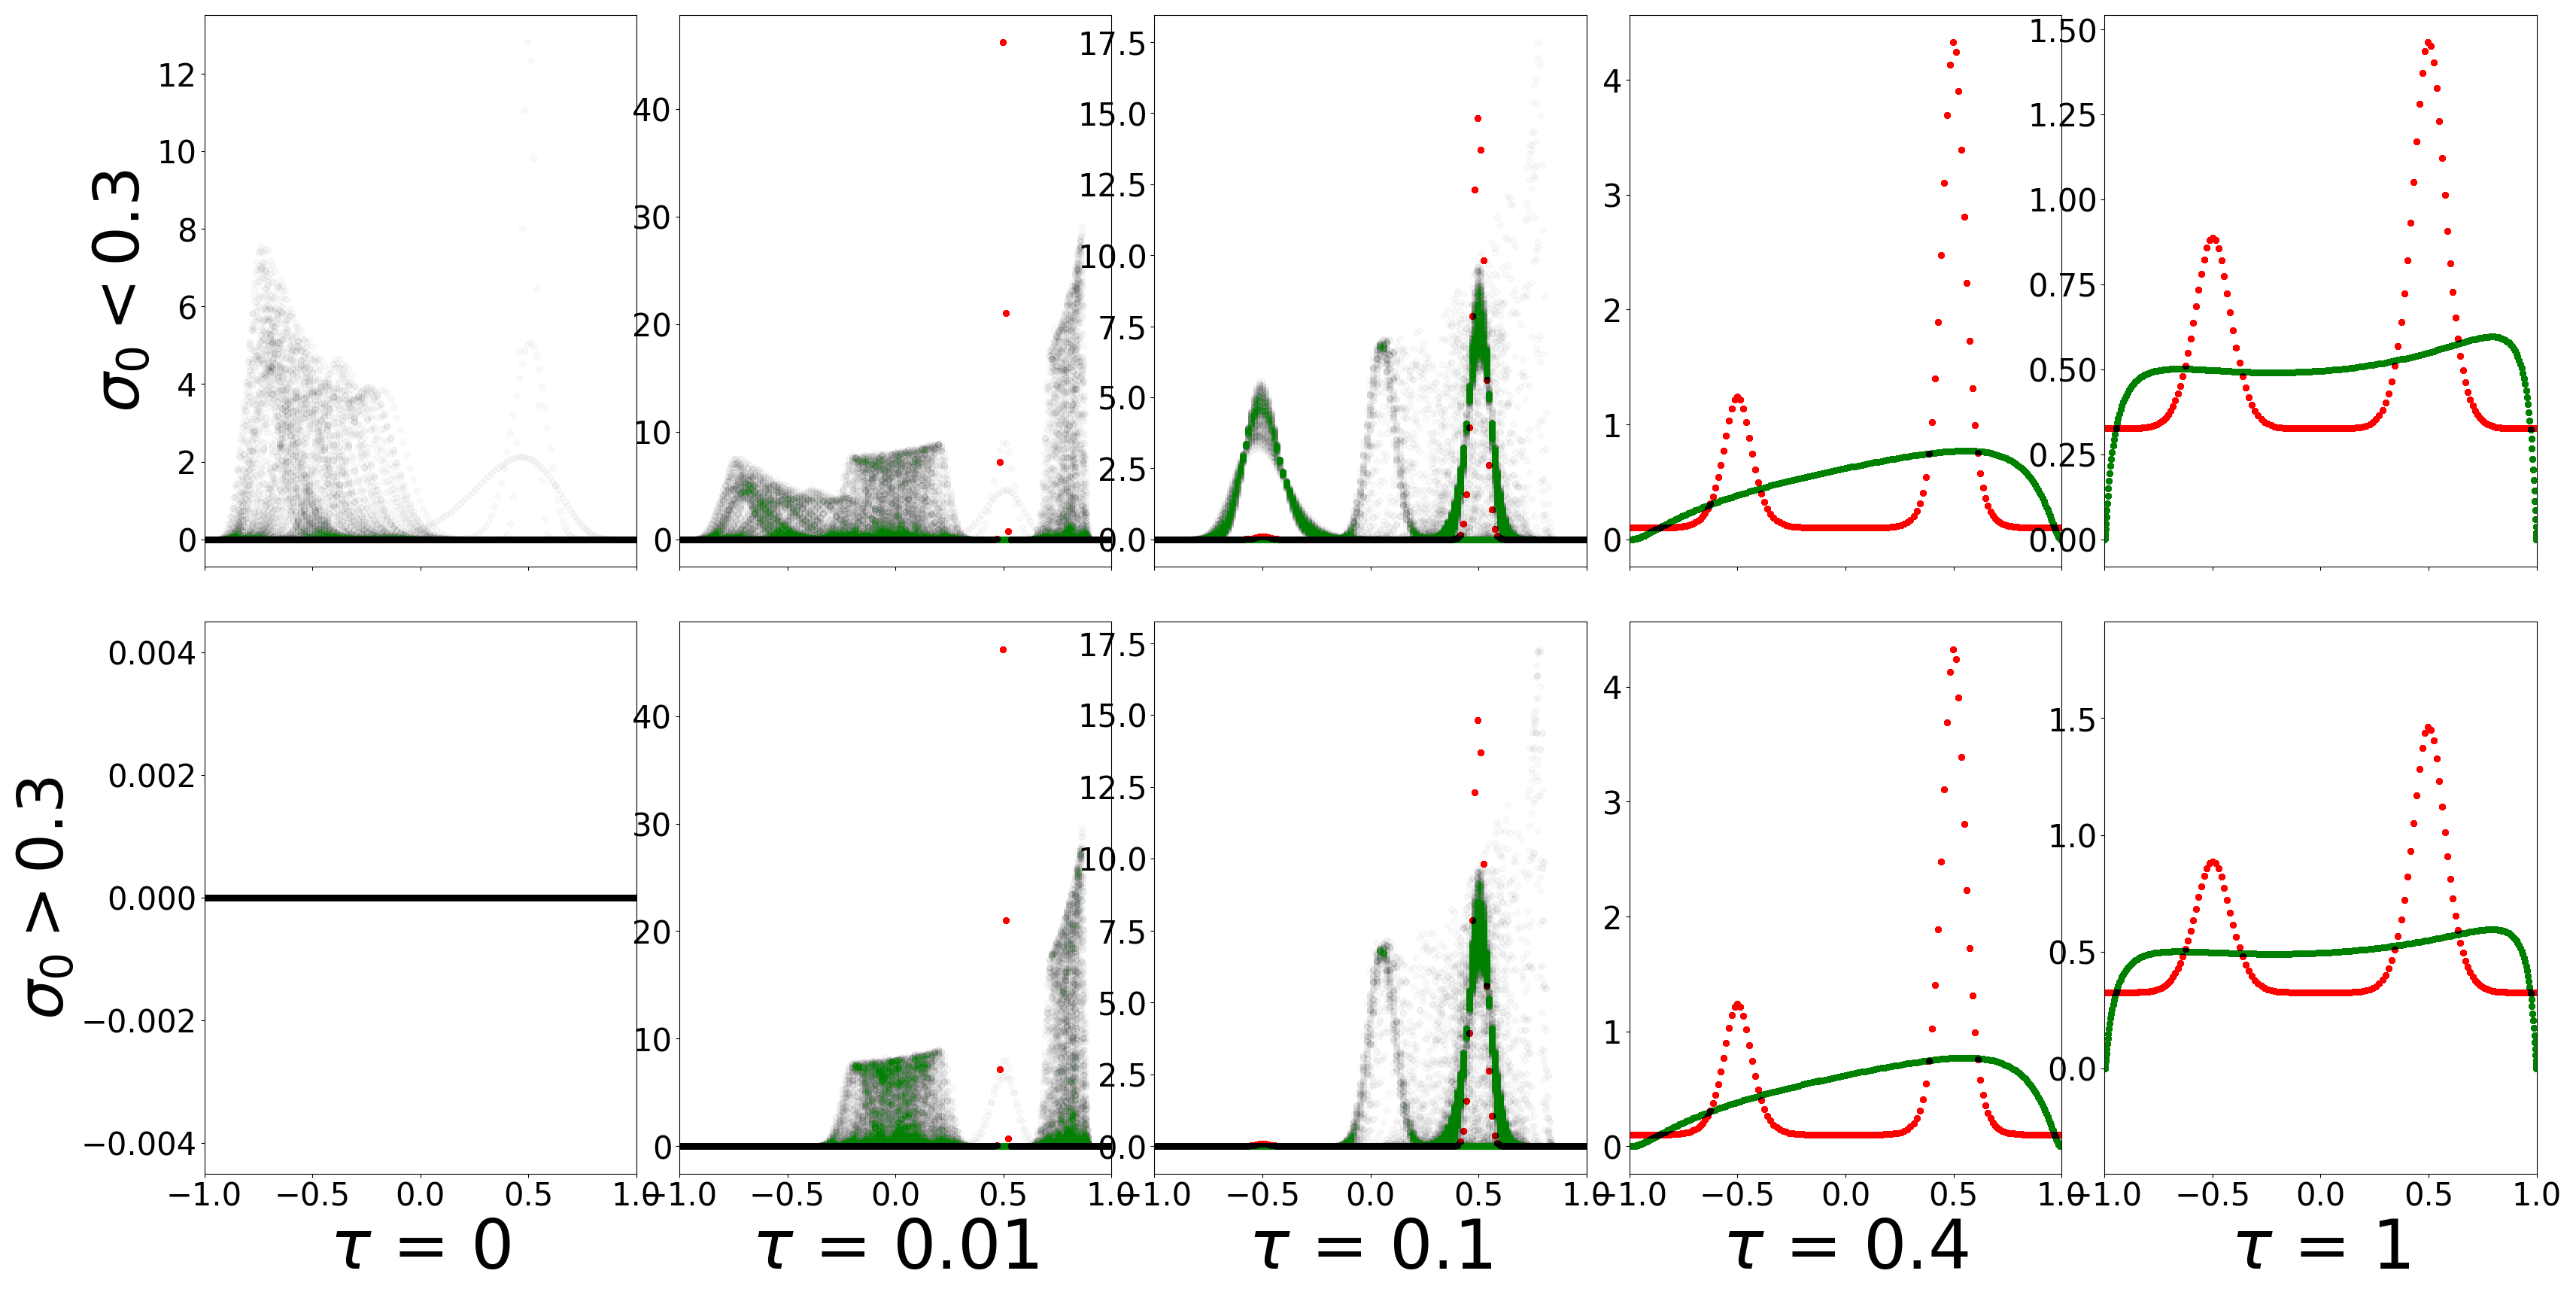
\includegraphics[width=1\columnwidth]{figs/bandit/notlearnQ/modes=1/sgd/pdf_forward_optim=sgd_modes=1_lr=0.01.png}
%     \caption{Forward KL, SGD.}
%     \label{fig:bandit-pdf-forward-sgd}
%   \end{subfigure}%
%   \begin{subfigure}[b]{0.4\linewidth}
%     \centering
%     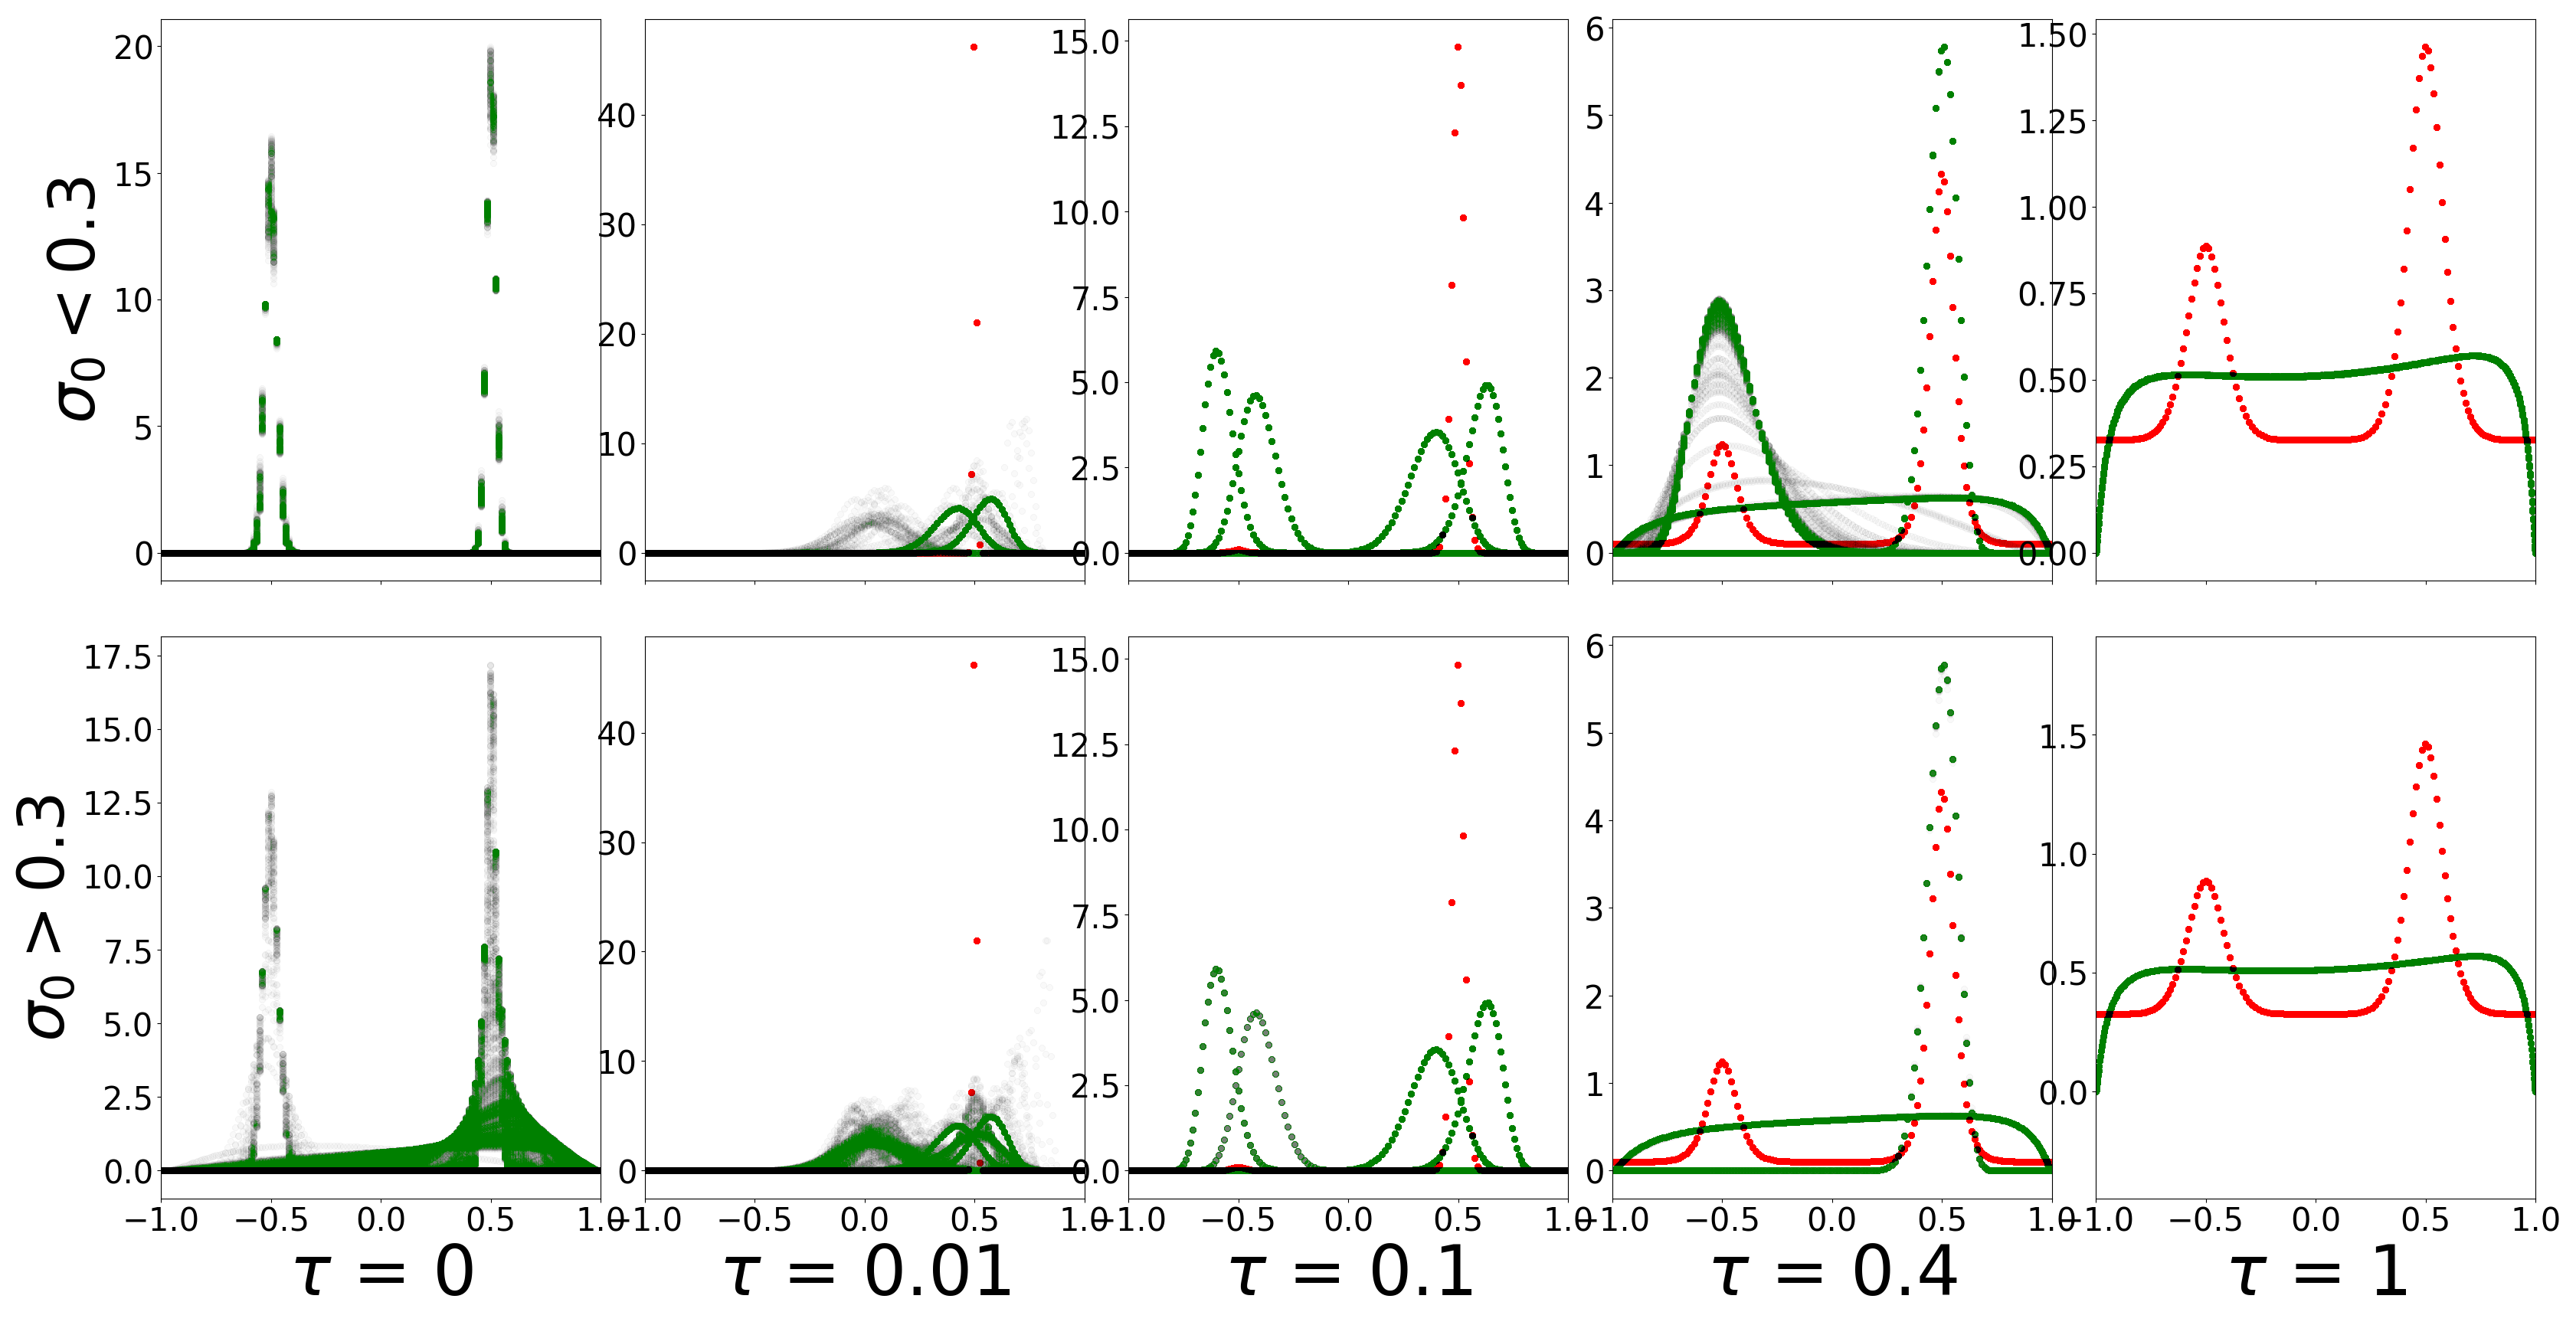
\includegraphics[width=1\columnwidth]{figs/bandit/notlearnQ/modes=1/sgd/pdf_reverse_optim=sgd_modes=1_lr=0.01.png}
%     \caption{Reverse KL, SGD.}
%     \label{fig:bandit-pdf-reverse-sgd}
%   \end{subfigure}
%   \caption{Final policy PDFs with unimodal policy. Red is the learned PDF of the policy and green is the target distribution. }
% \end{figure}

% \clearpage



% \clearpage

% % \subsection{Discrete Bandits - Optimization Path}\label{sec:discrete-bandit-plots}
% % Note that the maximum action for Hard FKL was set to be the third arm. 
% % \begin{figure}[!ht]
% %   \centering
% %   \begin{subfigure}[b]{0.4\linewidth}
% %     \centering
% %     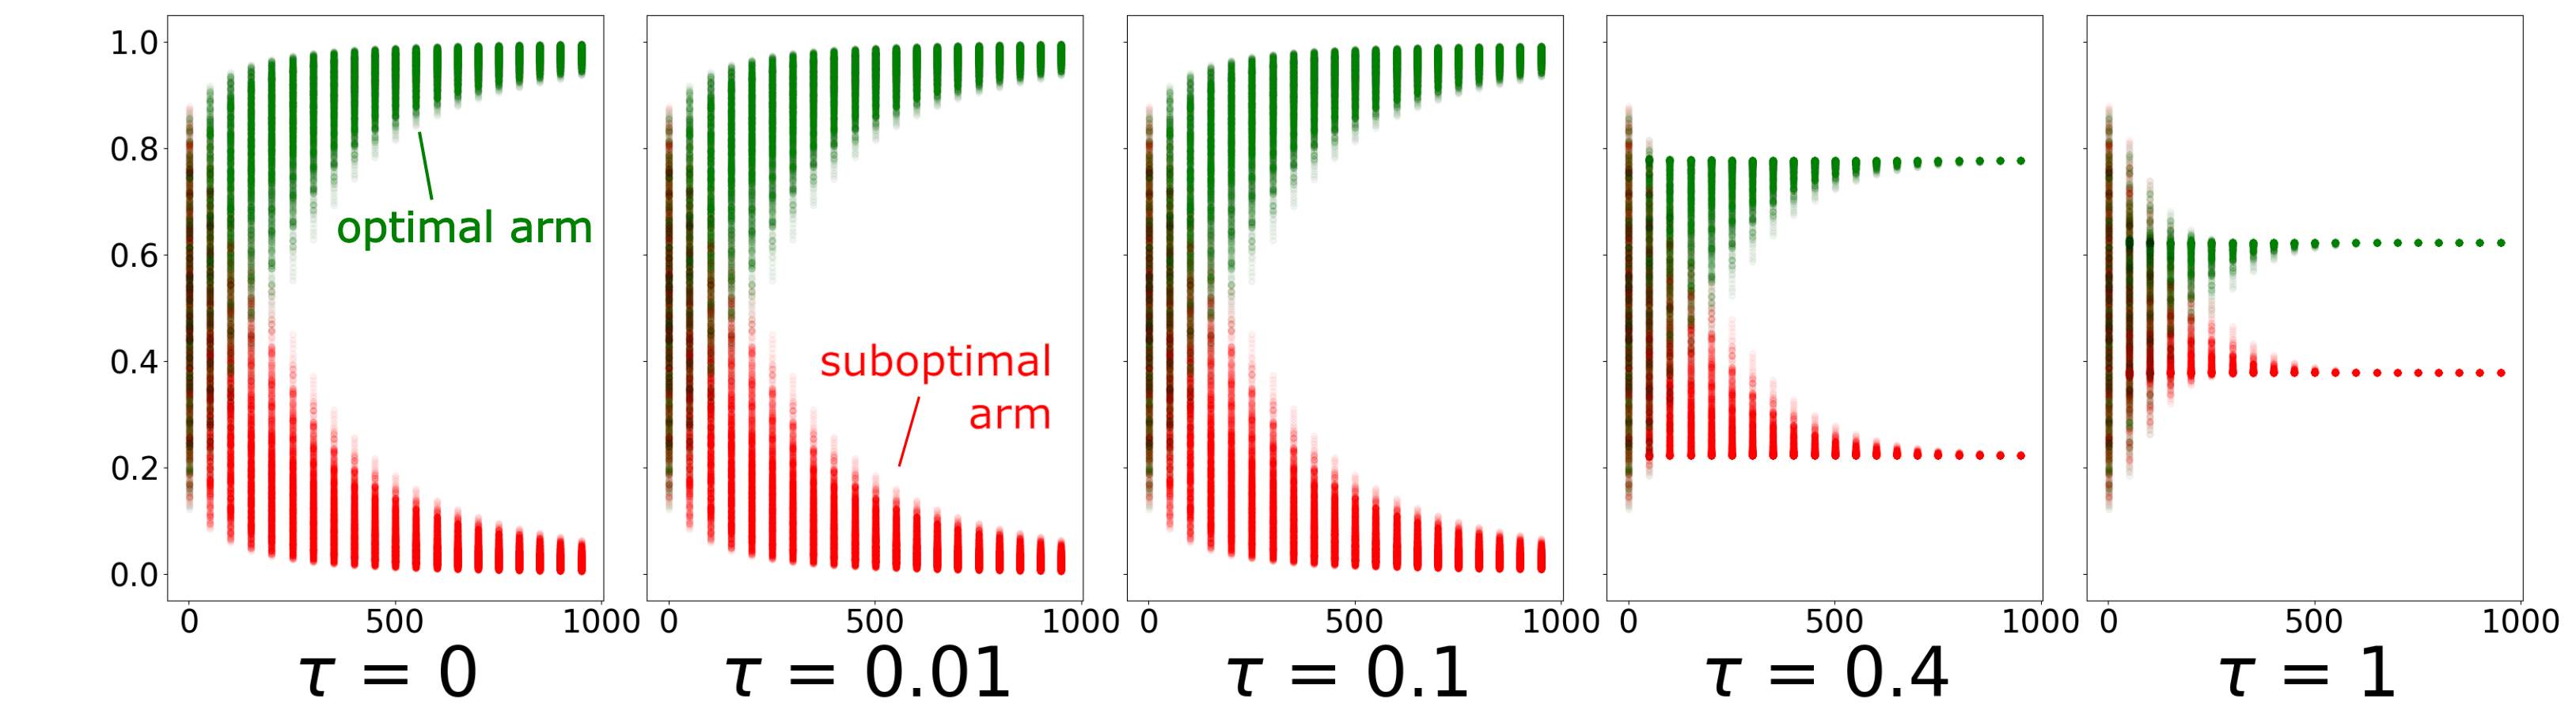
\includegraphics[width=1\columnwidth]{figs/discrete-bandit/notlearnQ/adam/prob-adam.png}
% %     \caption{Forward KL, Adam.}
% %     \label{fig:discrete-bandit-prob-forward-adam}
% %   \end{subfigure}%
% %   \begin{subfigure}[b]{0.4\linewidth}
% %     \centering
% %     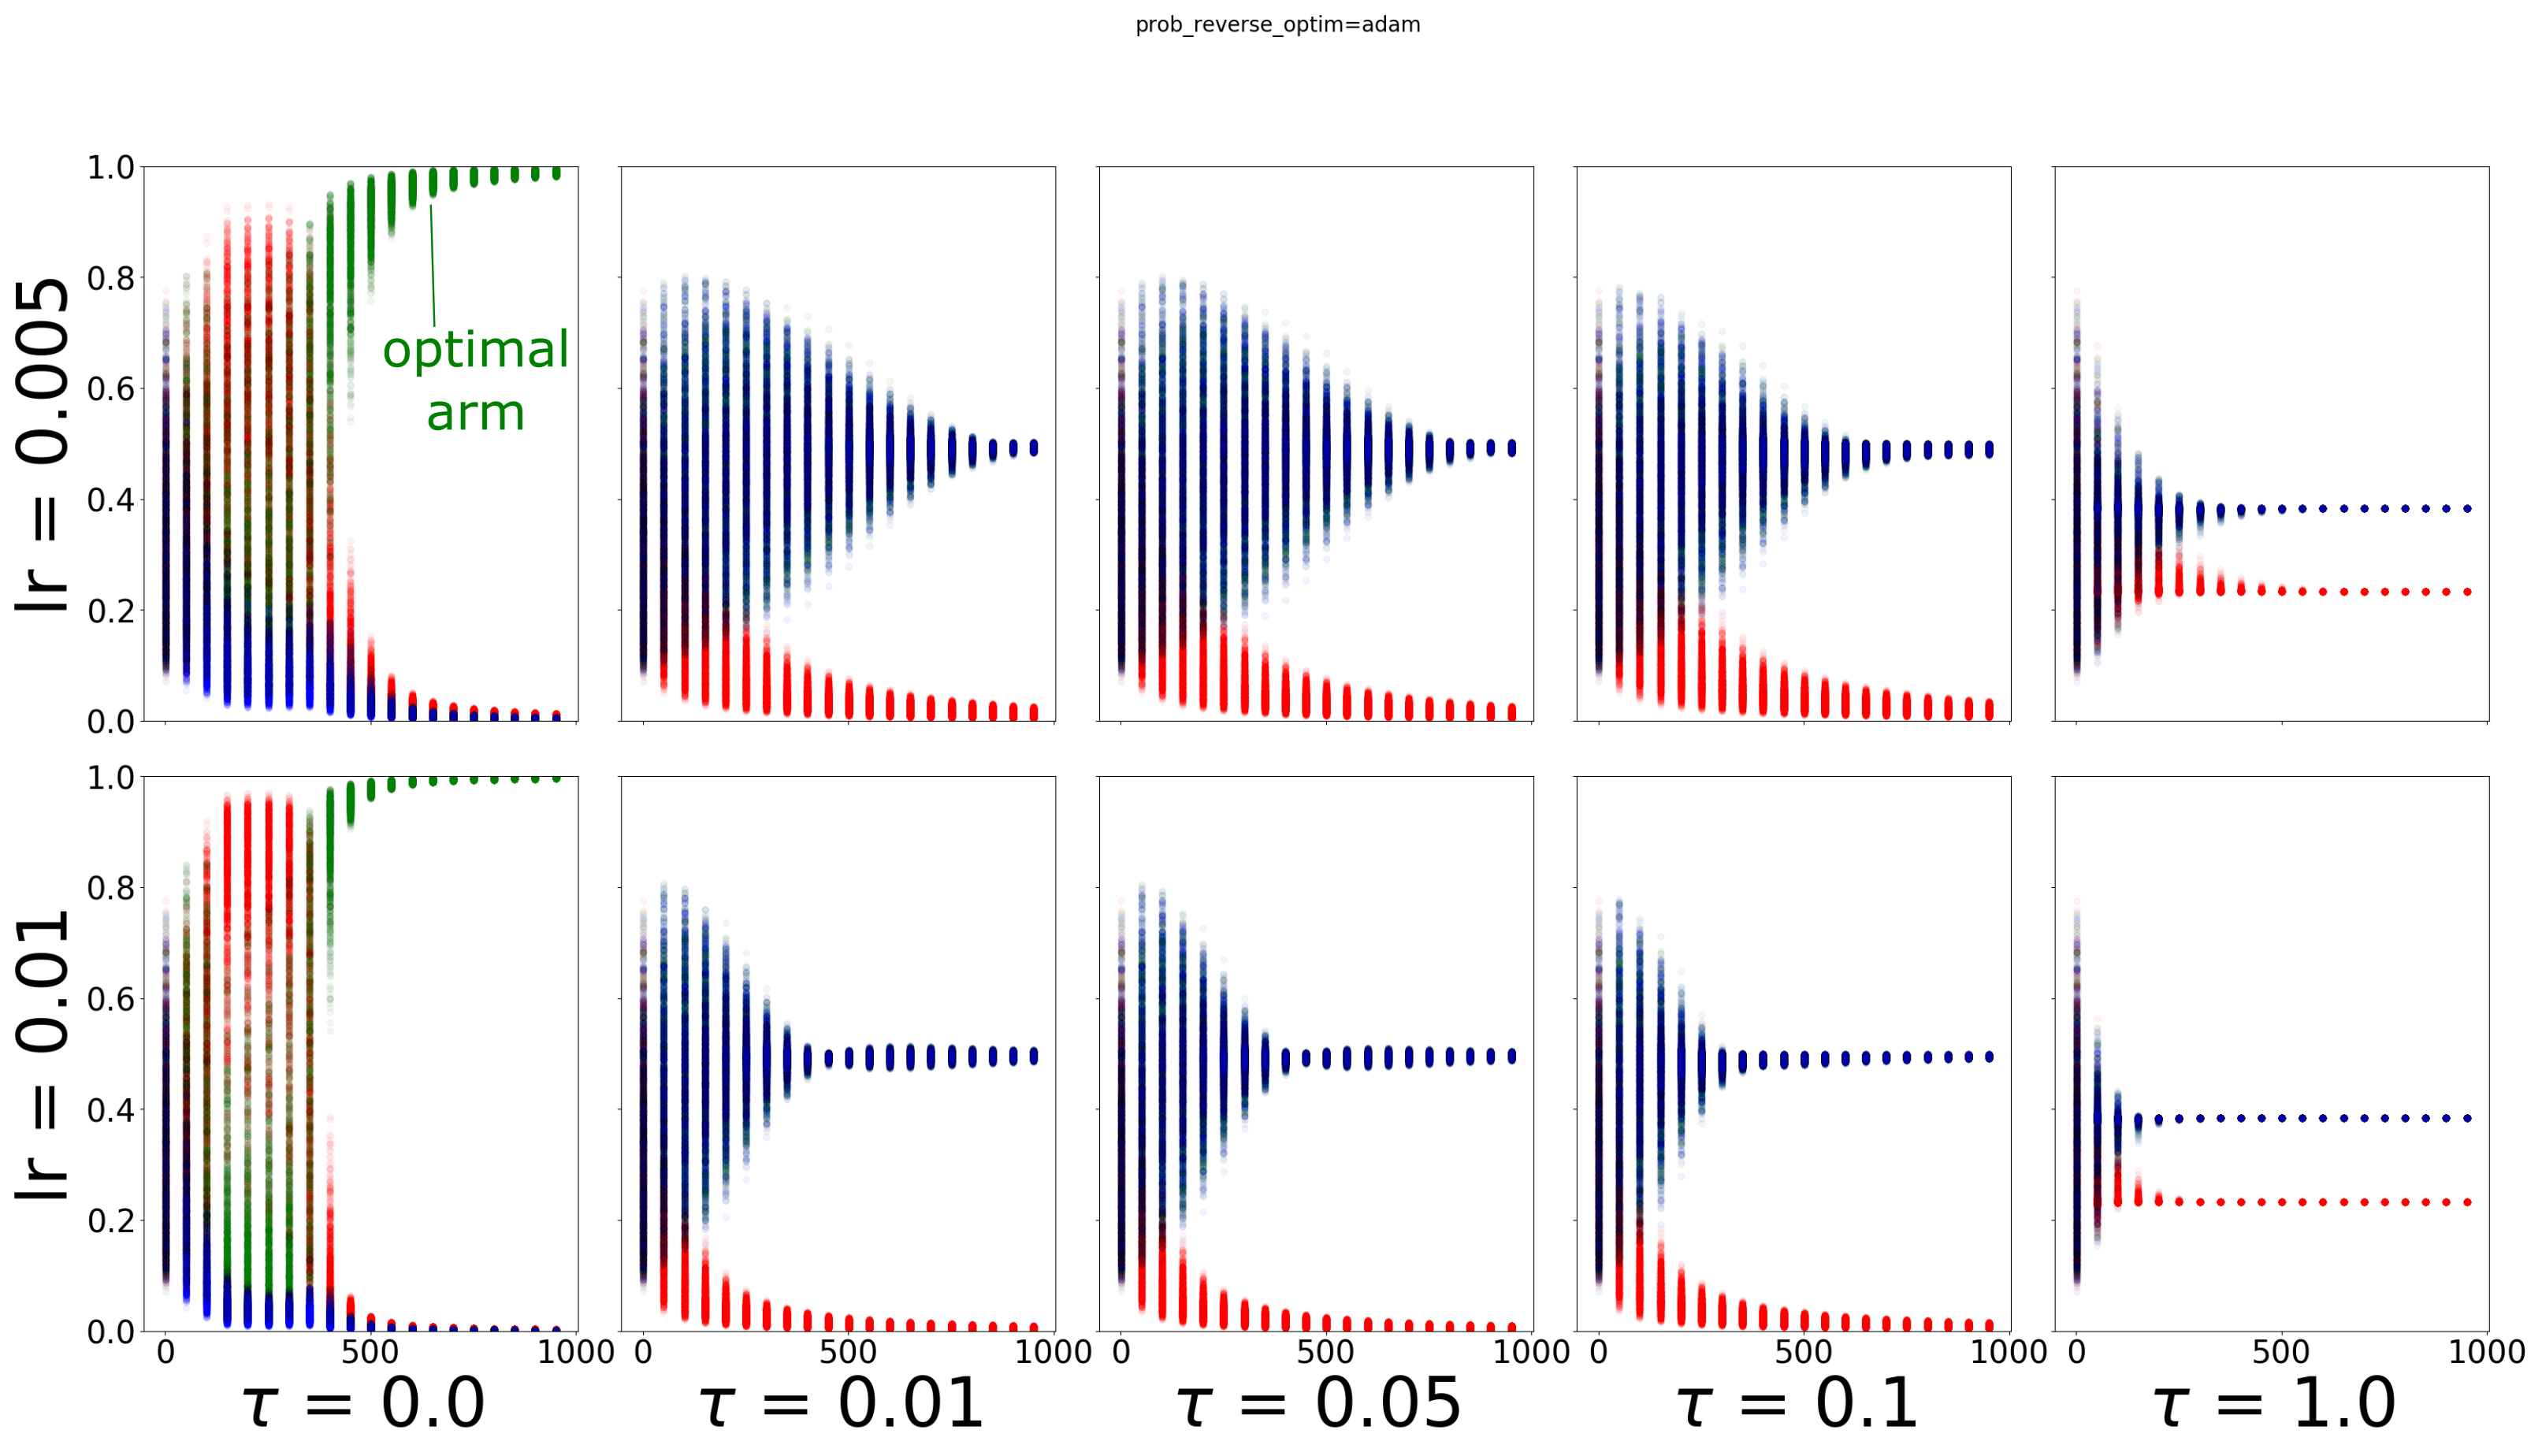
\includegraphics[width=1\columnwidth]{figs/discrete-bandit/notlearnQ/adam/prob-rev-adam.png}
% %     \caption{Reverse KL, Adam. }
% %     \label{fig:discrete-bandit-prob-reverse-adam}
% %   \end{subfigure}
  
% %   \begin{subfigure}[b]{0.4\linewidth}
% %     \centering
% %     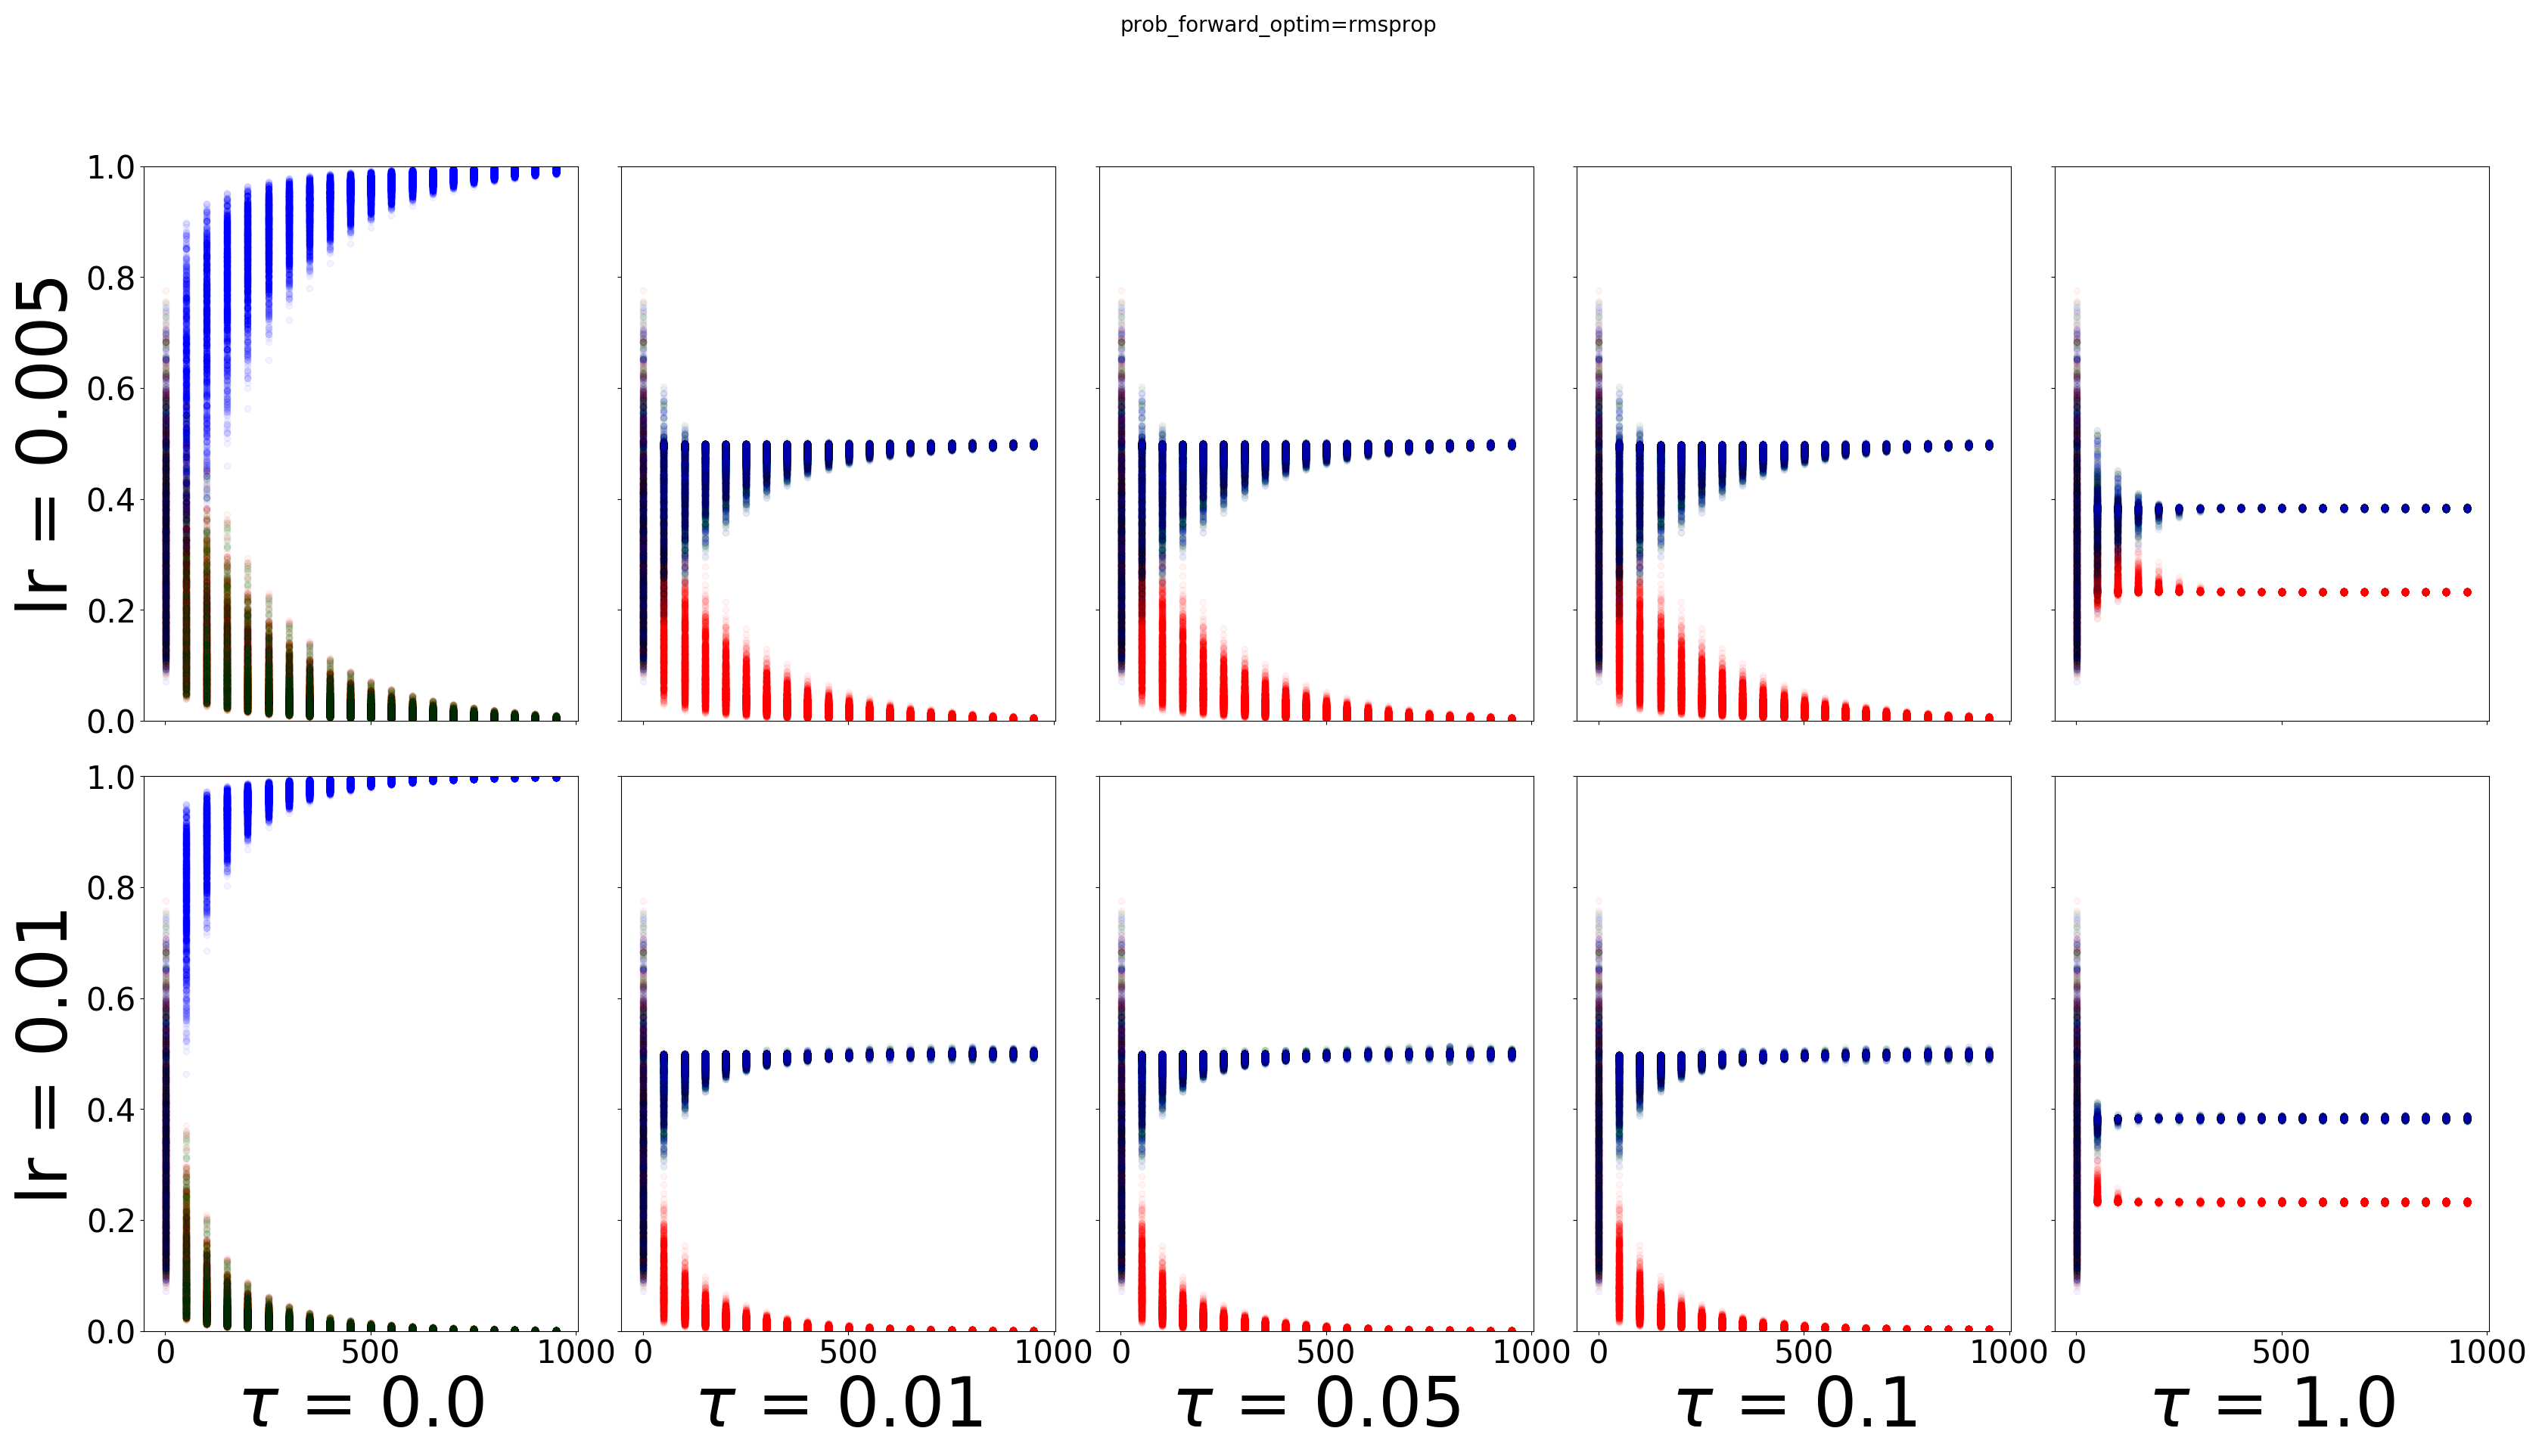
\includegraphics[width=1\columnwidth]{figs/discrete-bandit/notlearnQ/rmsprop/prob_forward_optim=rmsprop.png}
% %     \caption{Forward KL, RMSprop.}
% %     \label{fig:discrete-bandit-prob-forward-rmsprop}
% %   \end{subfigure}%
% %   \begin{subfigure}[b]{0.4\linewidth}
% %     \centering
% %     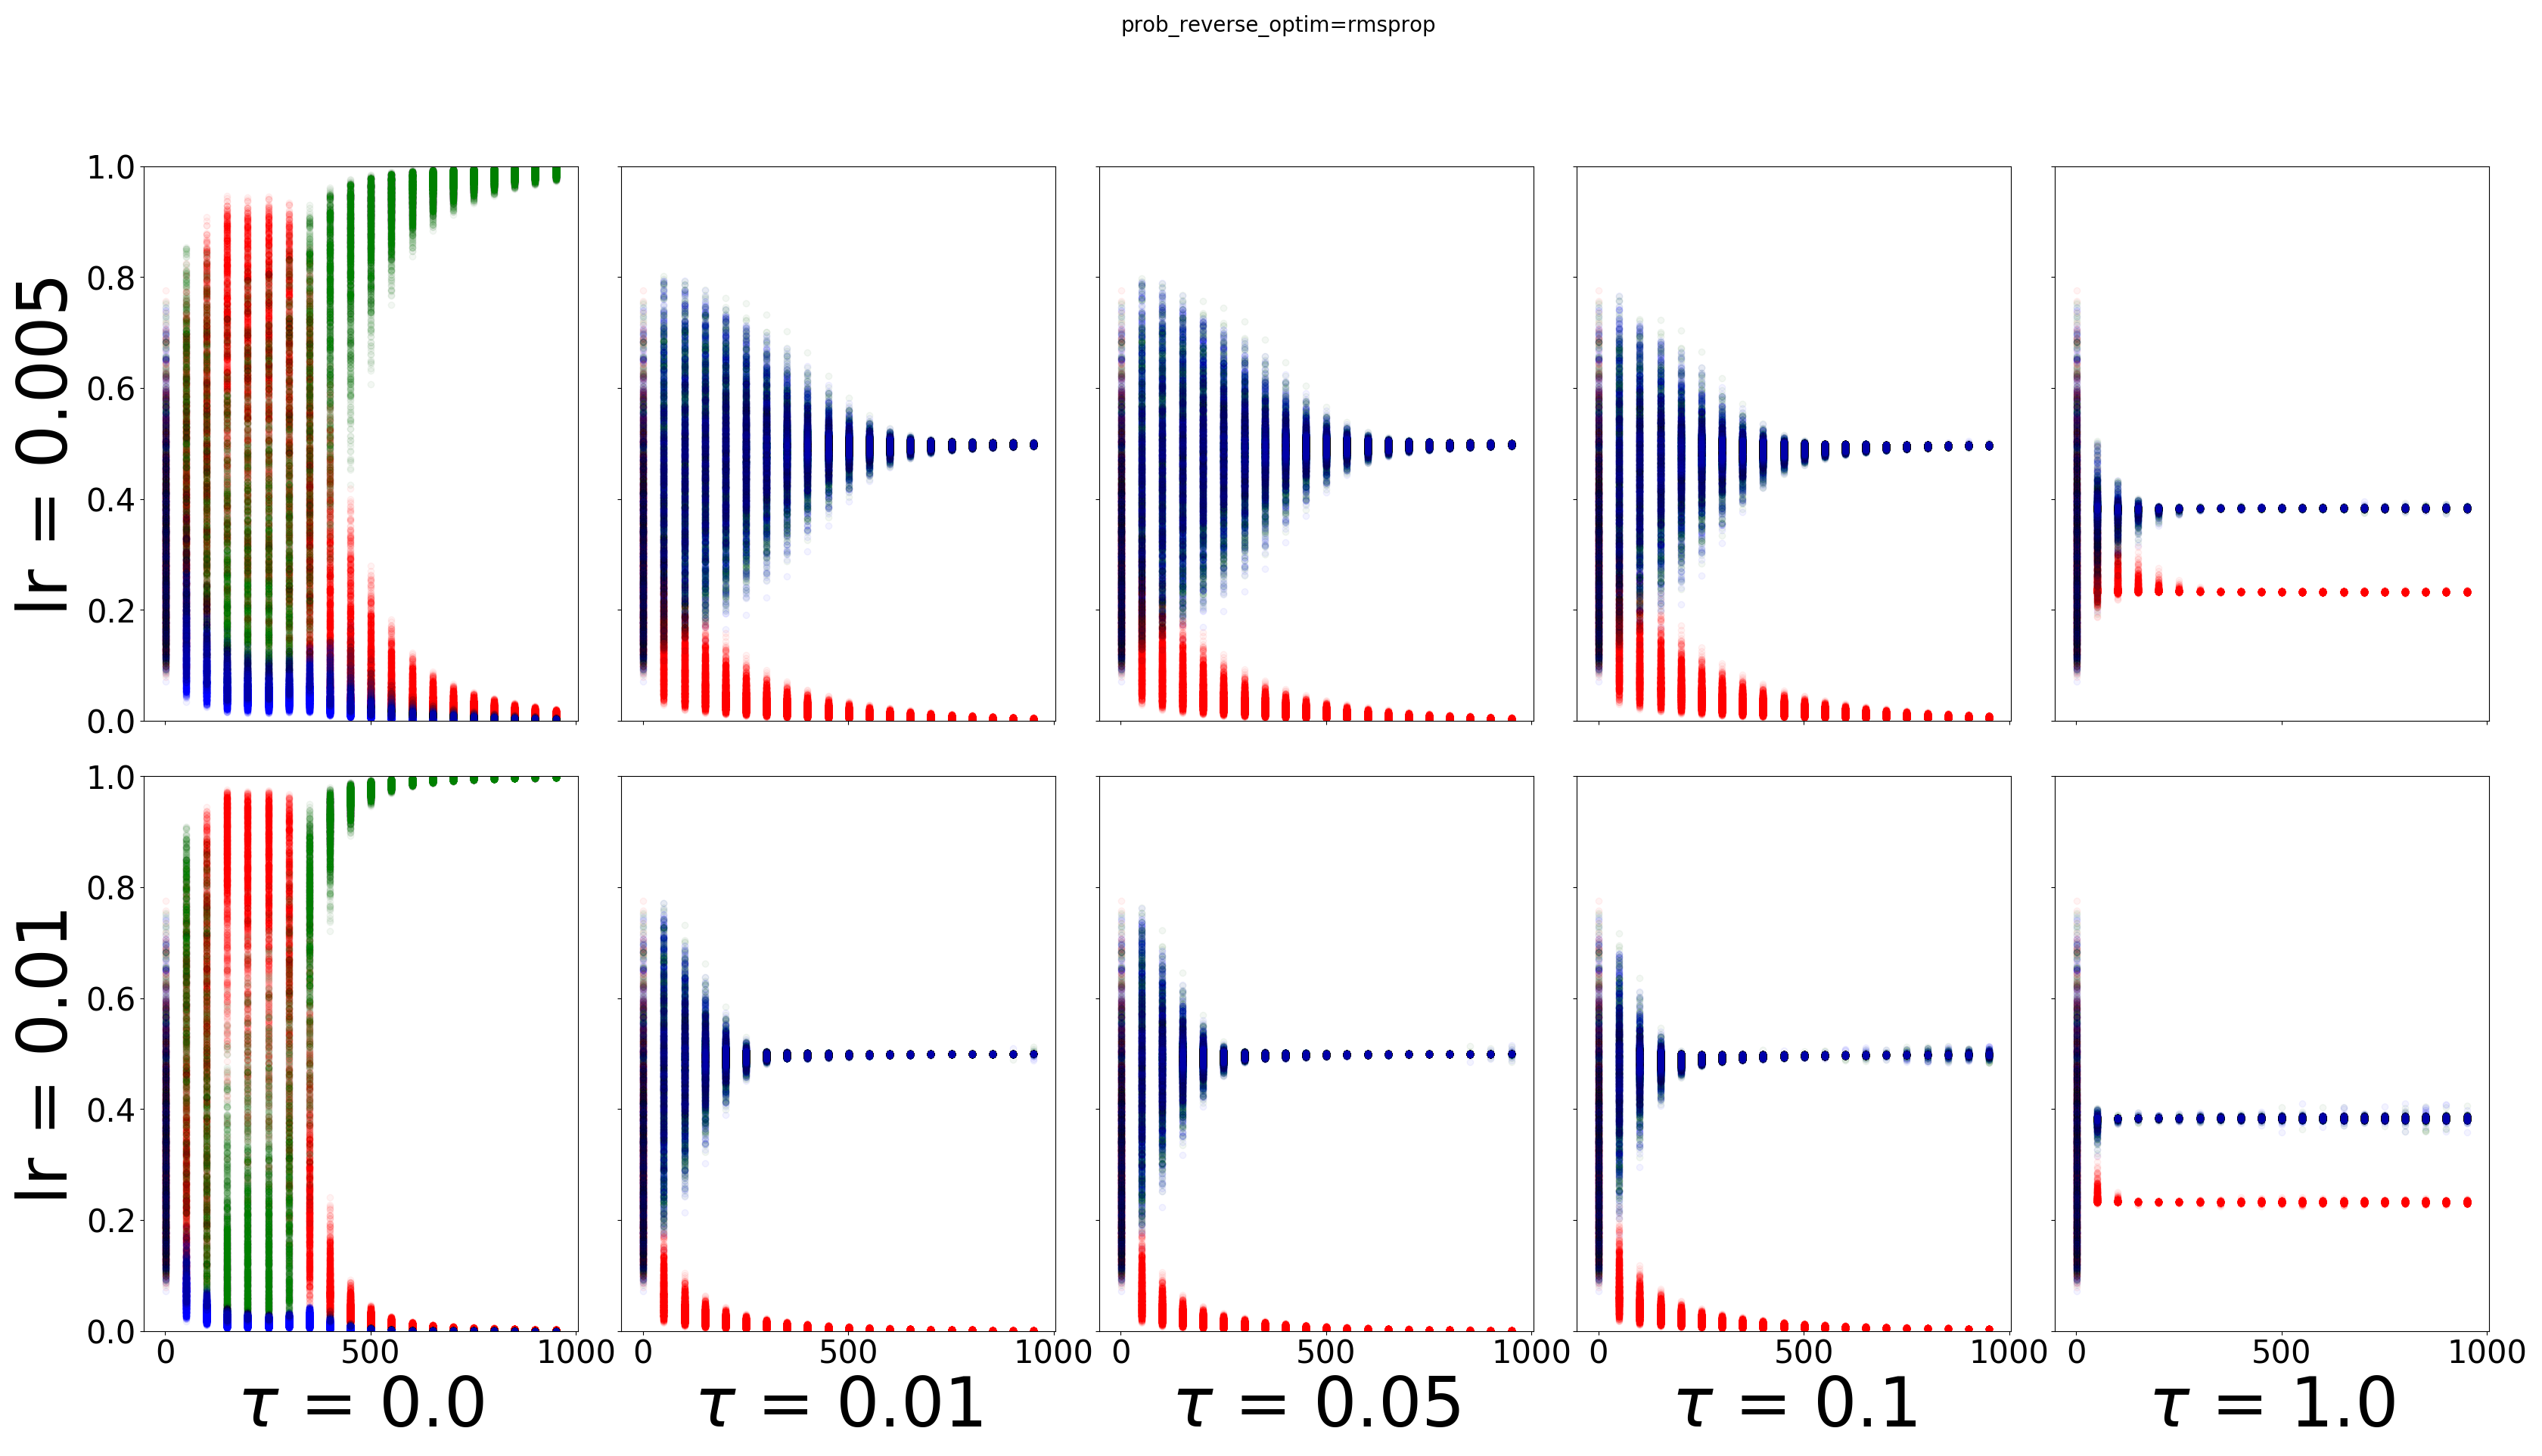
\includegraphics[width=1\columnwidth]{figs/discrete-bandit/notlearnQ/rmsprop/prob_reverse_optim=rmsprop.png}
% %     \caption{Reverse KL, RMSprop.}
% %     \label{fig:discrete-bandit-prob-reverse-rmsprop}
% %   \end{subfigure}
  
% %   \begin{subfigure}[b]{0.4\linewidth}
% %     \centering
% %     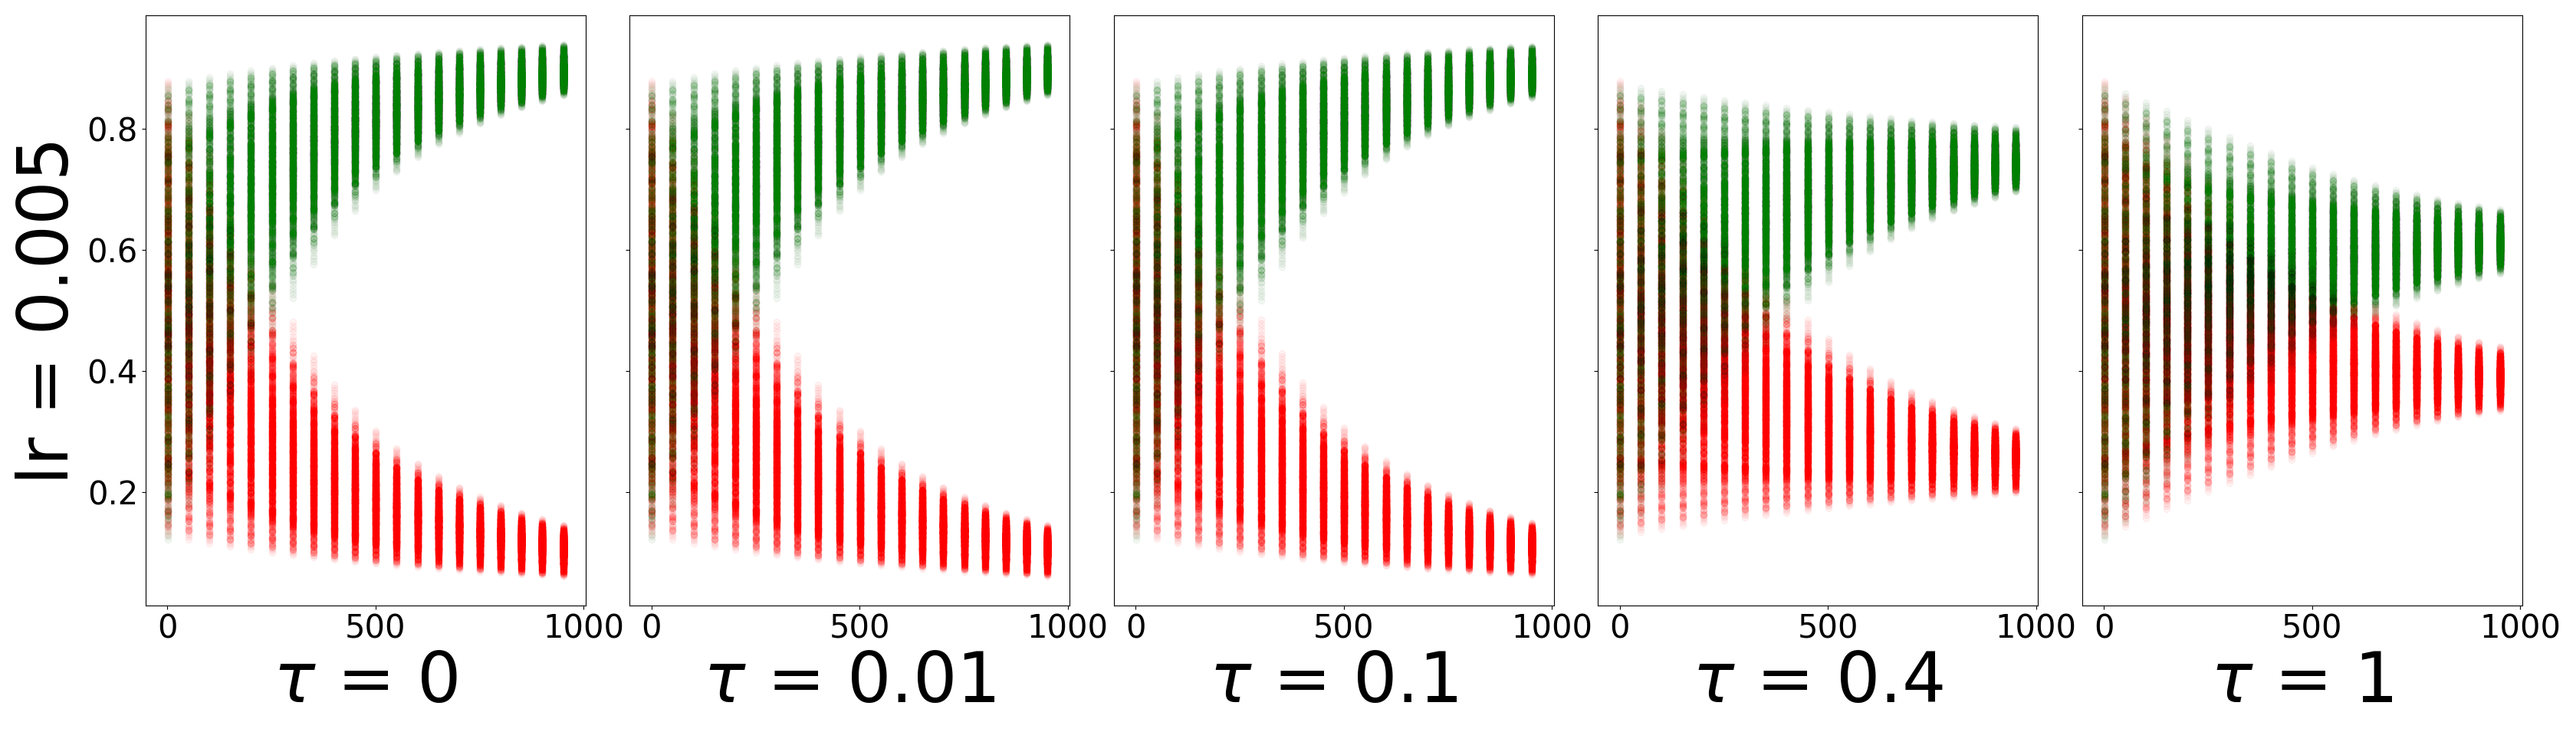
\includegraphics[width=1\columnwidth]{figs/discrete-bandit/notlearnQ/sgd/prob_forward_optim=sgd.png}
% %     \caption{Forward KL, SGD.}
% %     \label{fig:discrete-bandit-prob-forward-sgd}
% %   \end{subfigure}%
% %   \begin{subfigure}[b]{0.4\linewidth}
% %     \centering
% %     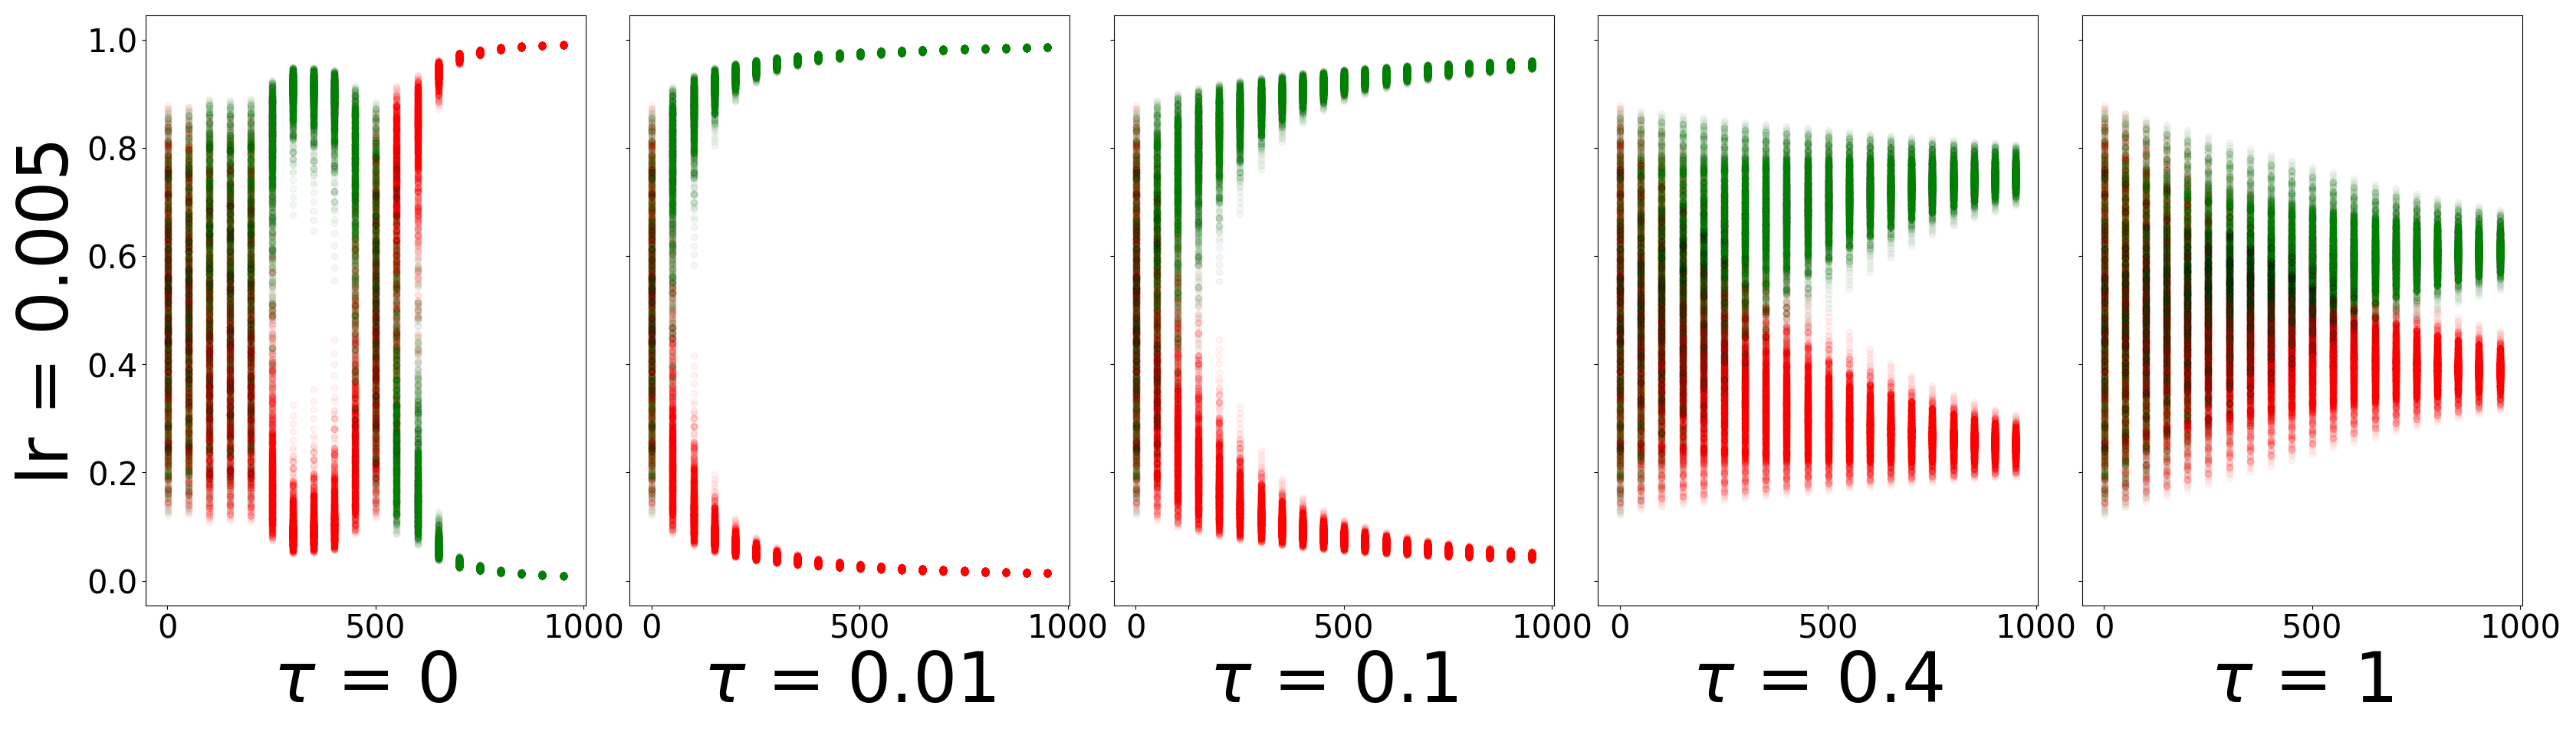
\includegraphics[width=1\columnwidth]{figs/discrete-bandit/notlearnQ/sgd/prob_reverse_optim=sgd.png}
% %     \caption{Reverse KL, SGD.}
% %     \label{fig:discrete-bandit-prob-reverse-sgd}
% %   \end{subfigure}
% %   \caption{Probability of each arm over time with softmax policy. Different colours are different modes. }
% % \end{figure}

% % % \begin{figure}[!ht]
% % %   \centering
% % %   \begin{subfigure}[b]{0.4\linewidth}
% % %     \centering
% % %     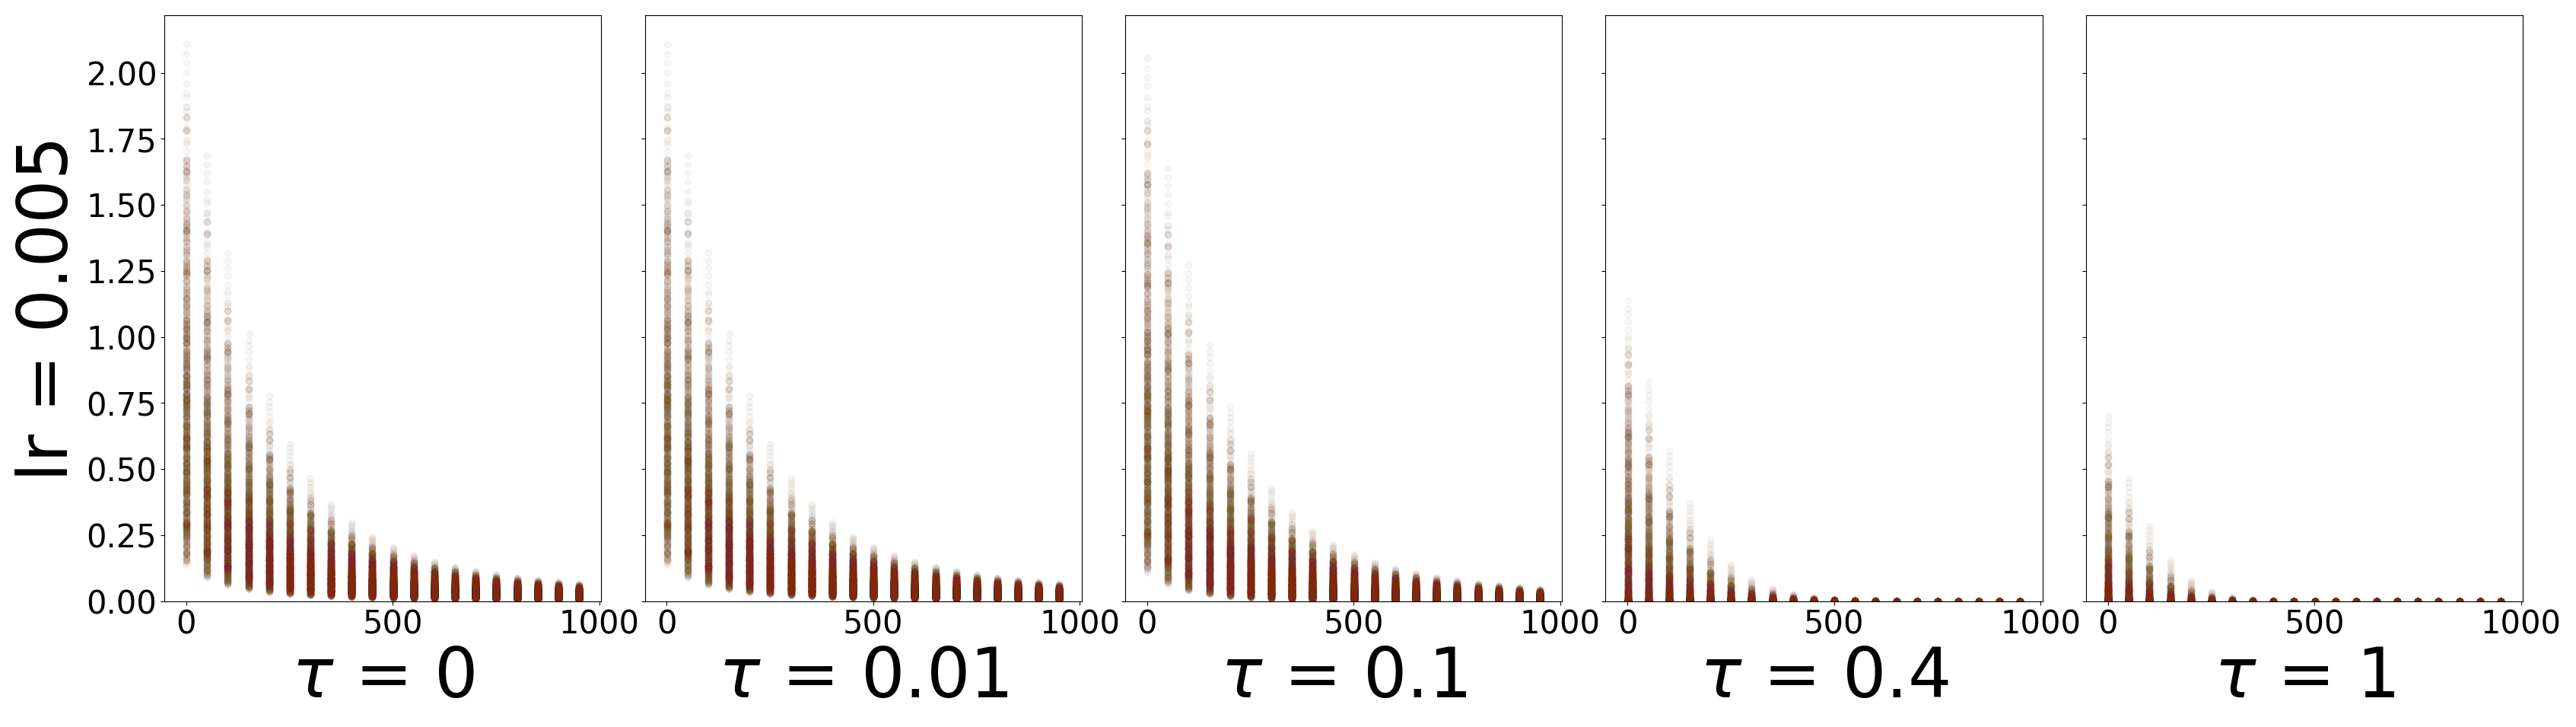
\includegraphics[width=1\columnwidth]{figs/discrete-bandit/notlearnQ/adam/loss_forward_optim=adam.png}
% % %     \caption{Forward KL, Adam.}
% % %     \label{fig:discrete-bandit-loss-forward-adam}
% % %   \end{subfigure}%
% % %   \begin{subfigure}[b]{0.4\linewidth}
% % %     \centering
% % %     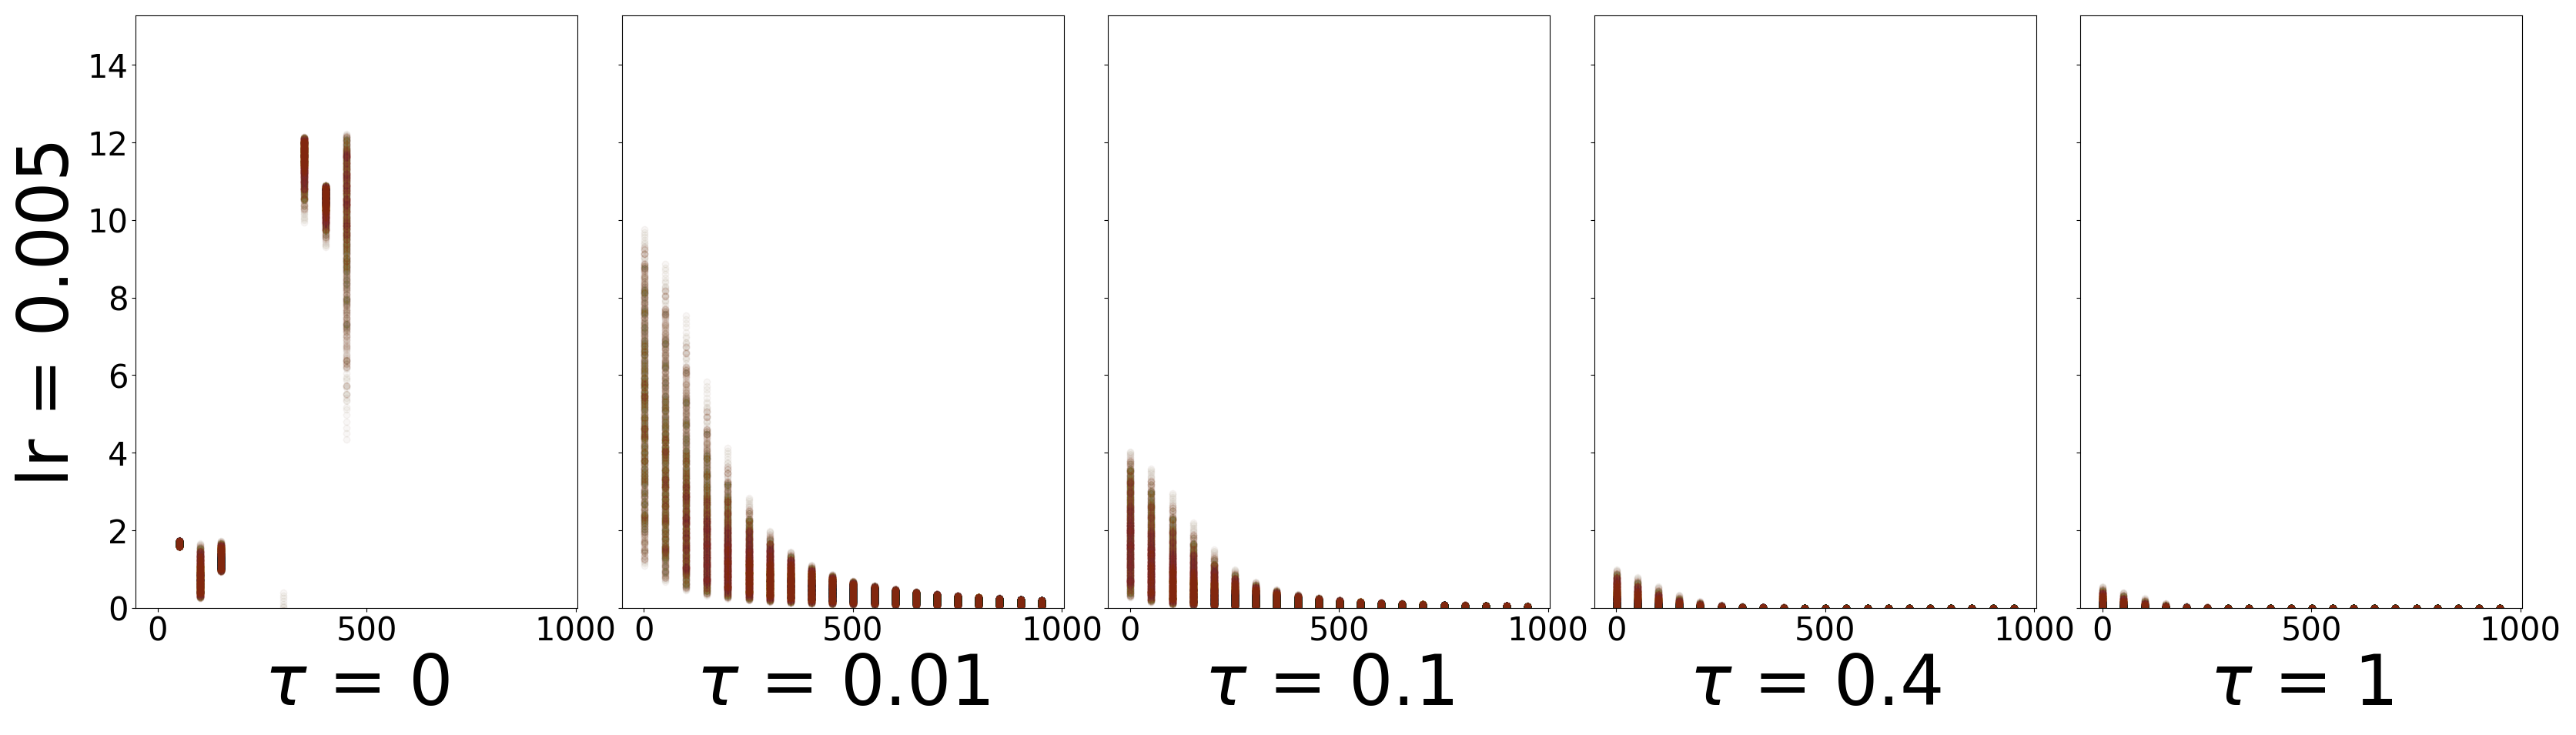
\includegraphics[width=1\columnwidth]{figs/discrete-bandit/notlearnQ/adam/loss_reverse_optim=adam.png}
% % %     \caption{Reverse KL, Adam. }
% % %     \label{fig:discrete-bandit-loss-reverse-adam}
% % %   \end{subfigure}
  
% % %   \begin{subfigure}[b]{0.4\linewidth}
% % %     \centering
% % %     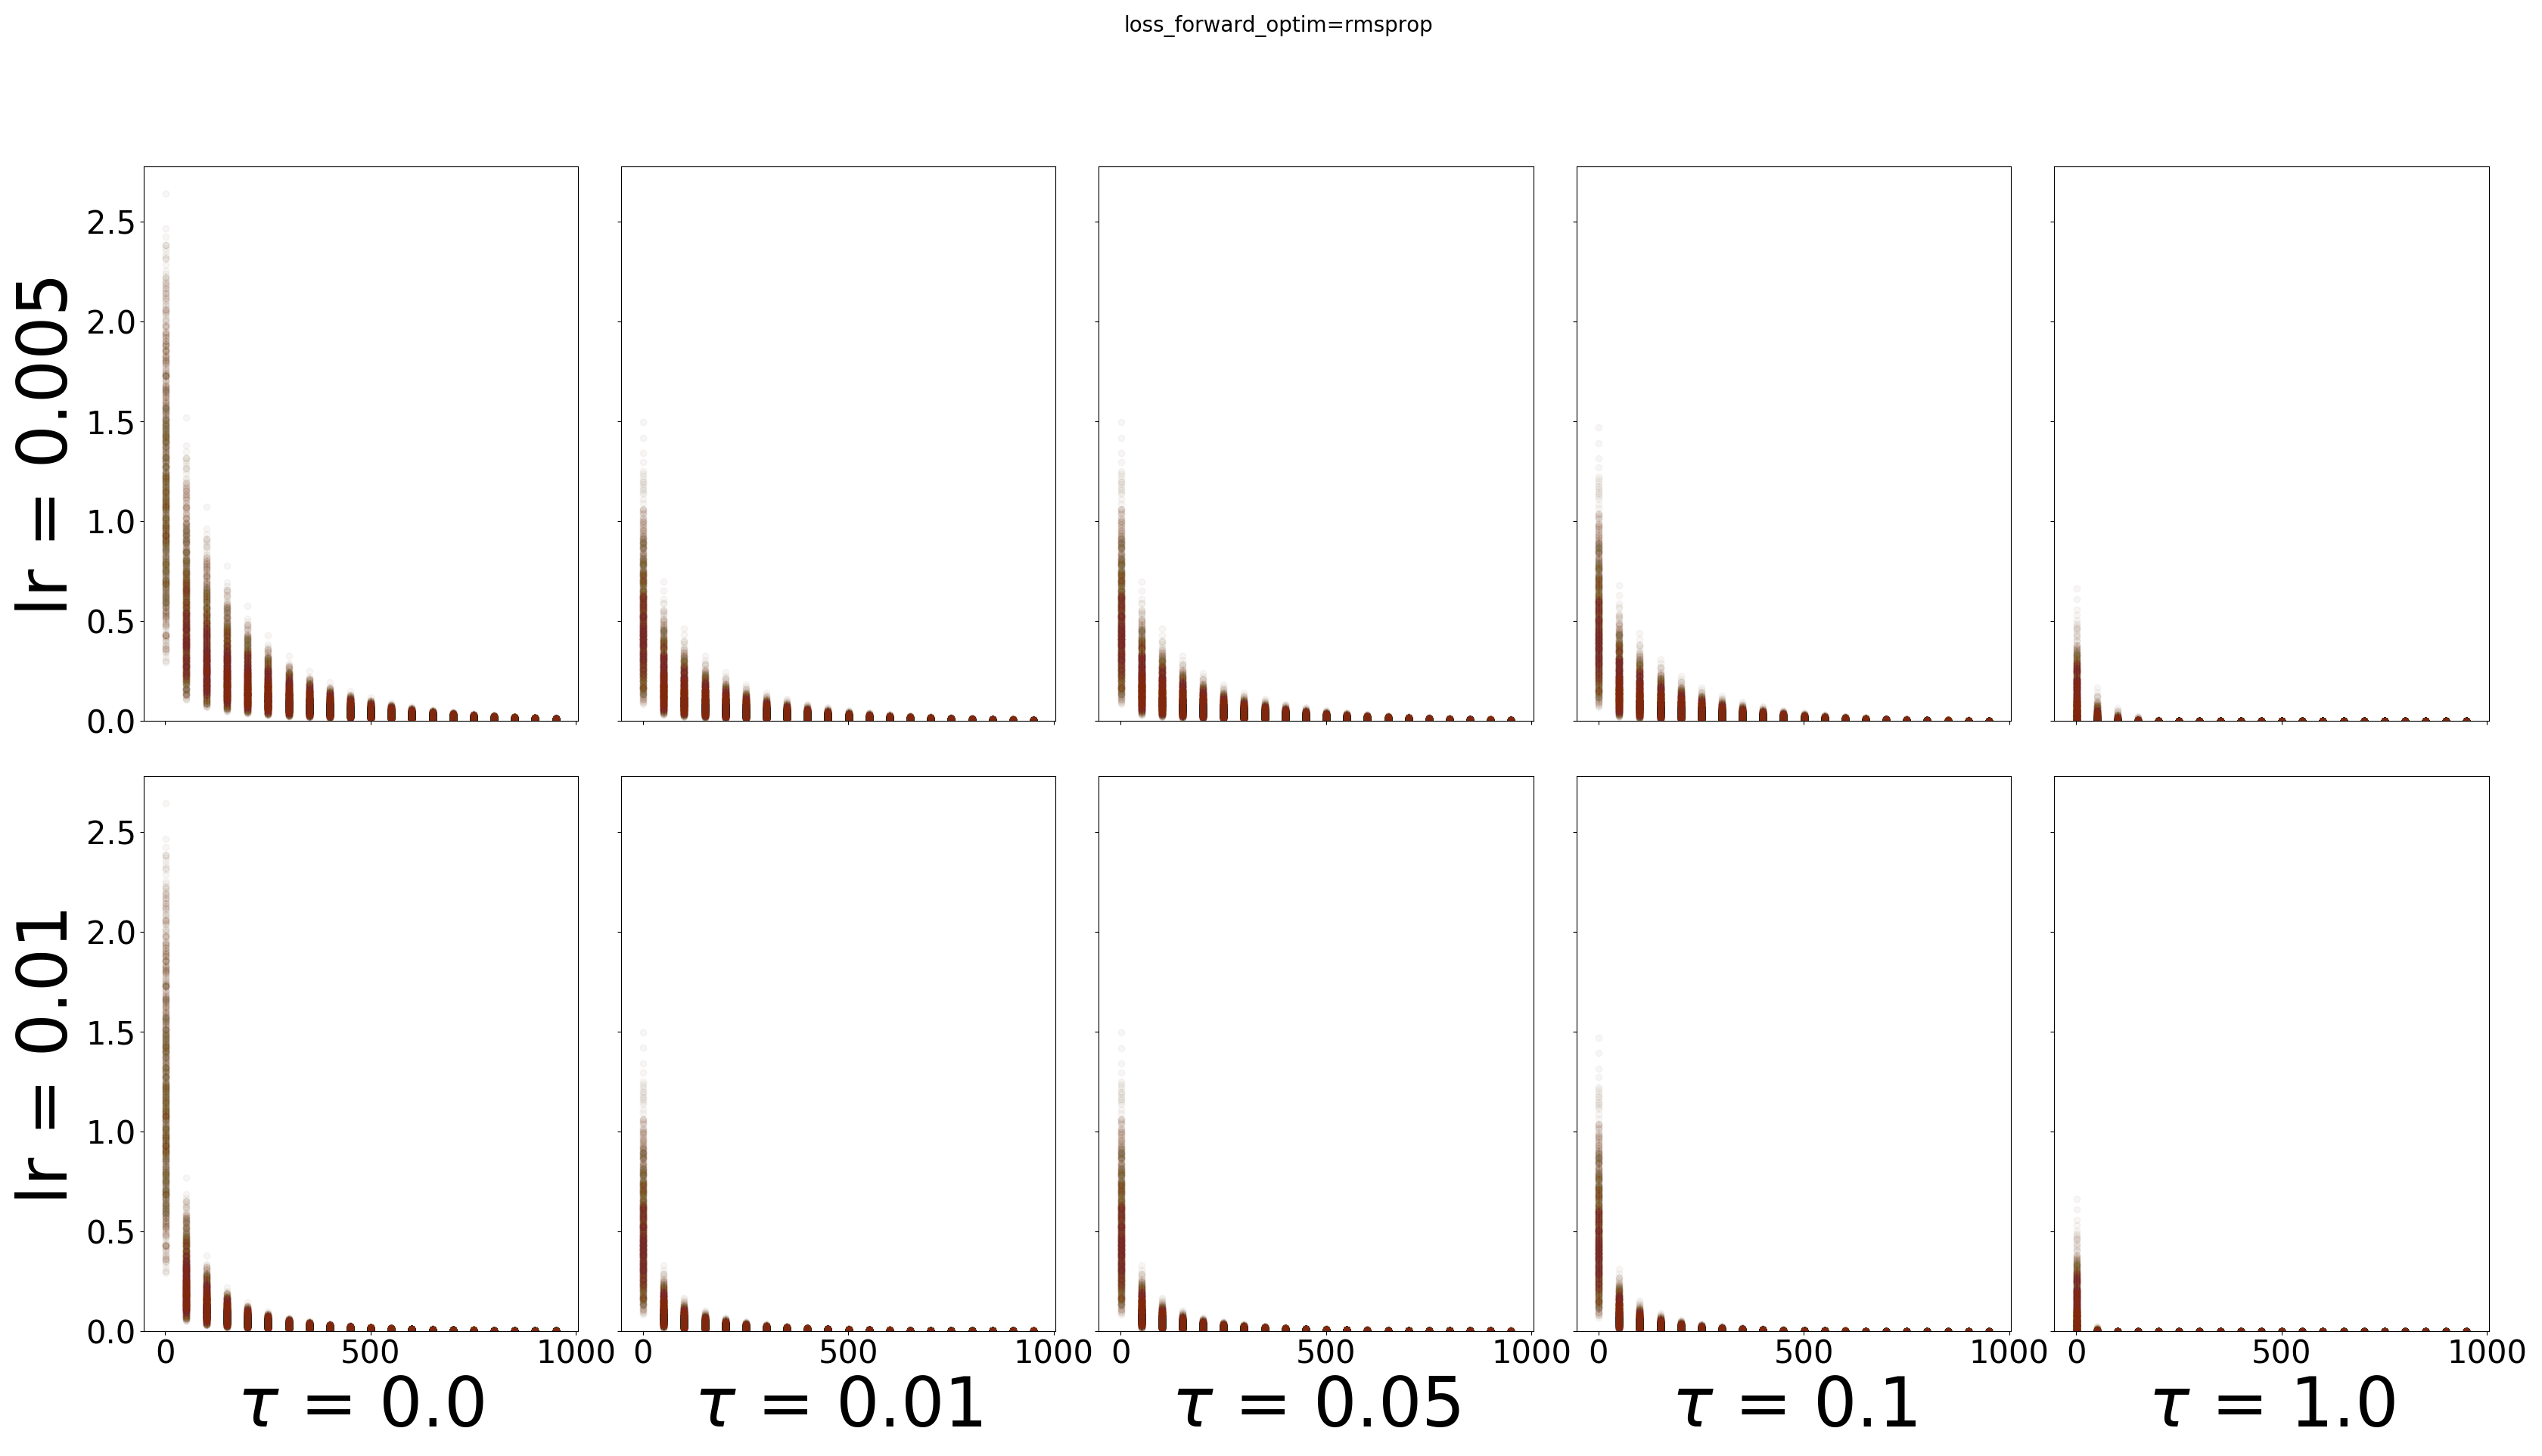
\includegraphics[width=1\columnwidth]{figs/discrete-bandit/notlearnQ/rmsprop/loss_forward_optim=rmsprop.png}
% % %     \caption{Forward KL, RMSprop.}
% % %     \label{fig:discrete-bandit-loss-forward-rmsprop}
% % %   \end{subfigure}%
% % %   \begin{subfigure}[b]{0.4\linewidth}
% % %     \centering
% % %     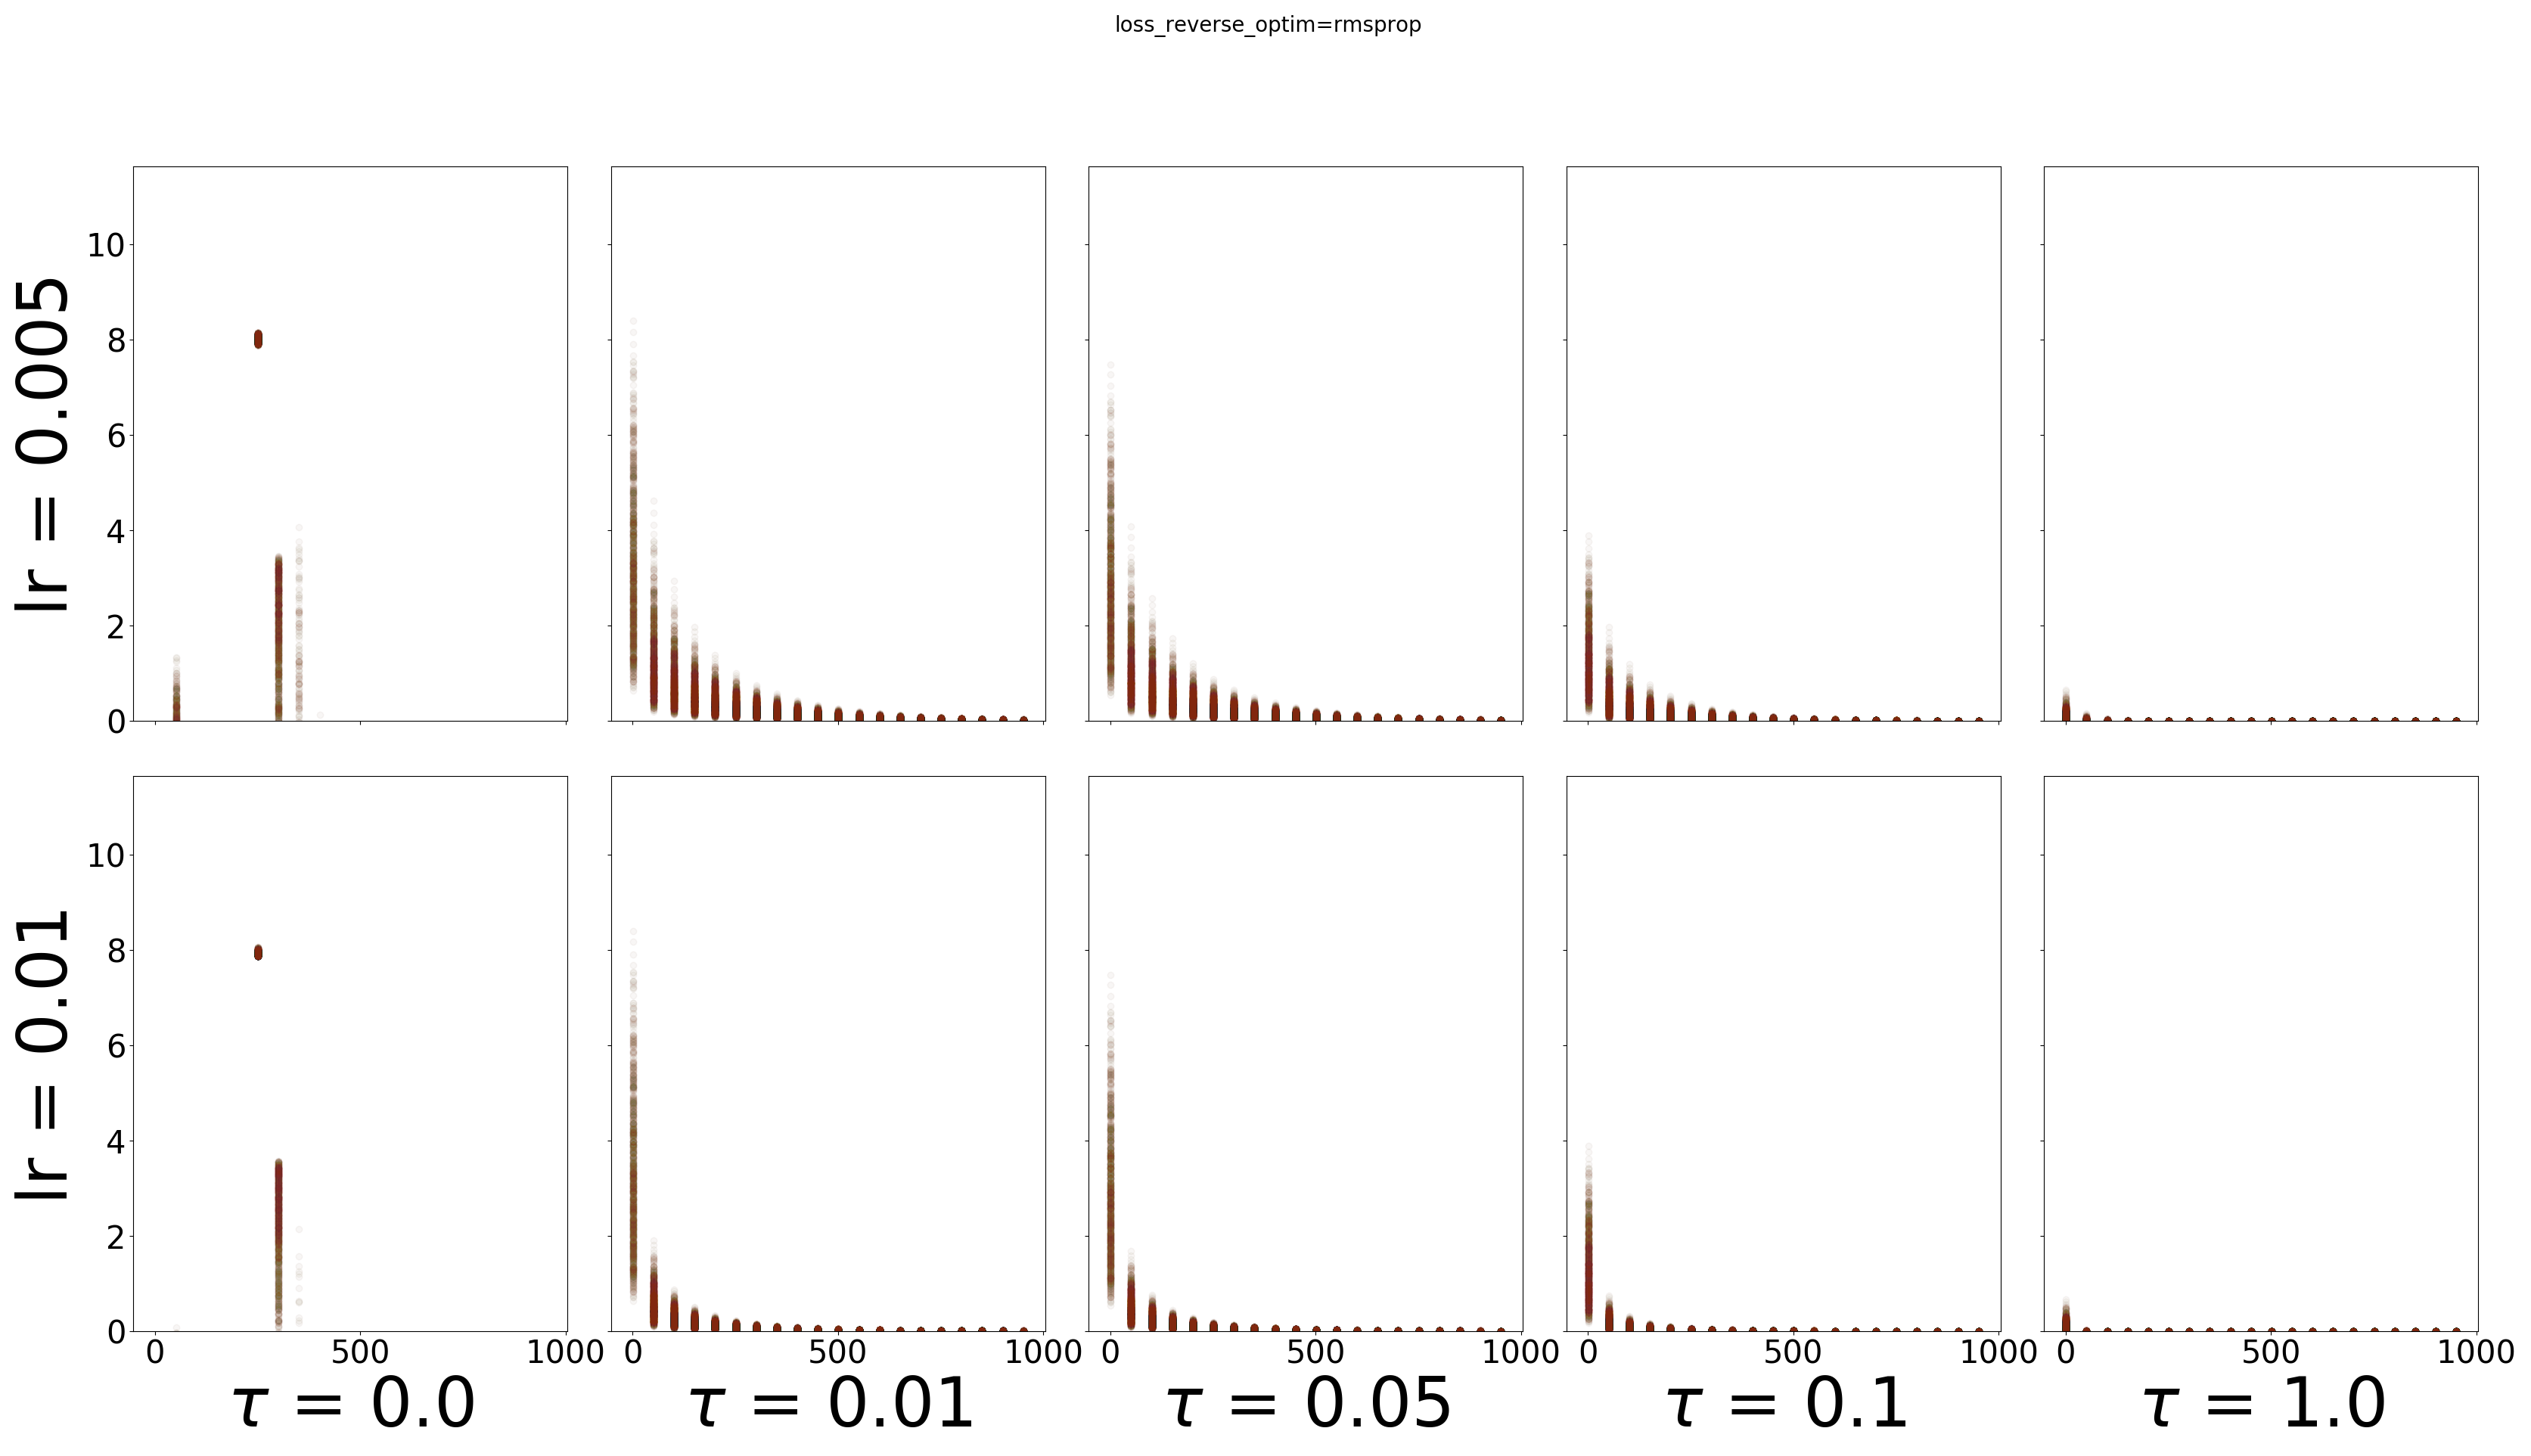
\includegraphics[width=1\columnwidth]{figs/discrete-bandit/notlearnQ/rmsprop/loss_reverse_optim=rmsprop.png}
% % %     \caption{Reverse KL, RMSprop.}
% % %     \label{fig:discrete-bandit-loss-reverse-rmsprop}
% % %   \end{subfigure}
  
% % %   \begin{subfigure}[b]{0.4\linewidth}
% % %     \centering
% % %     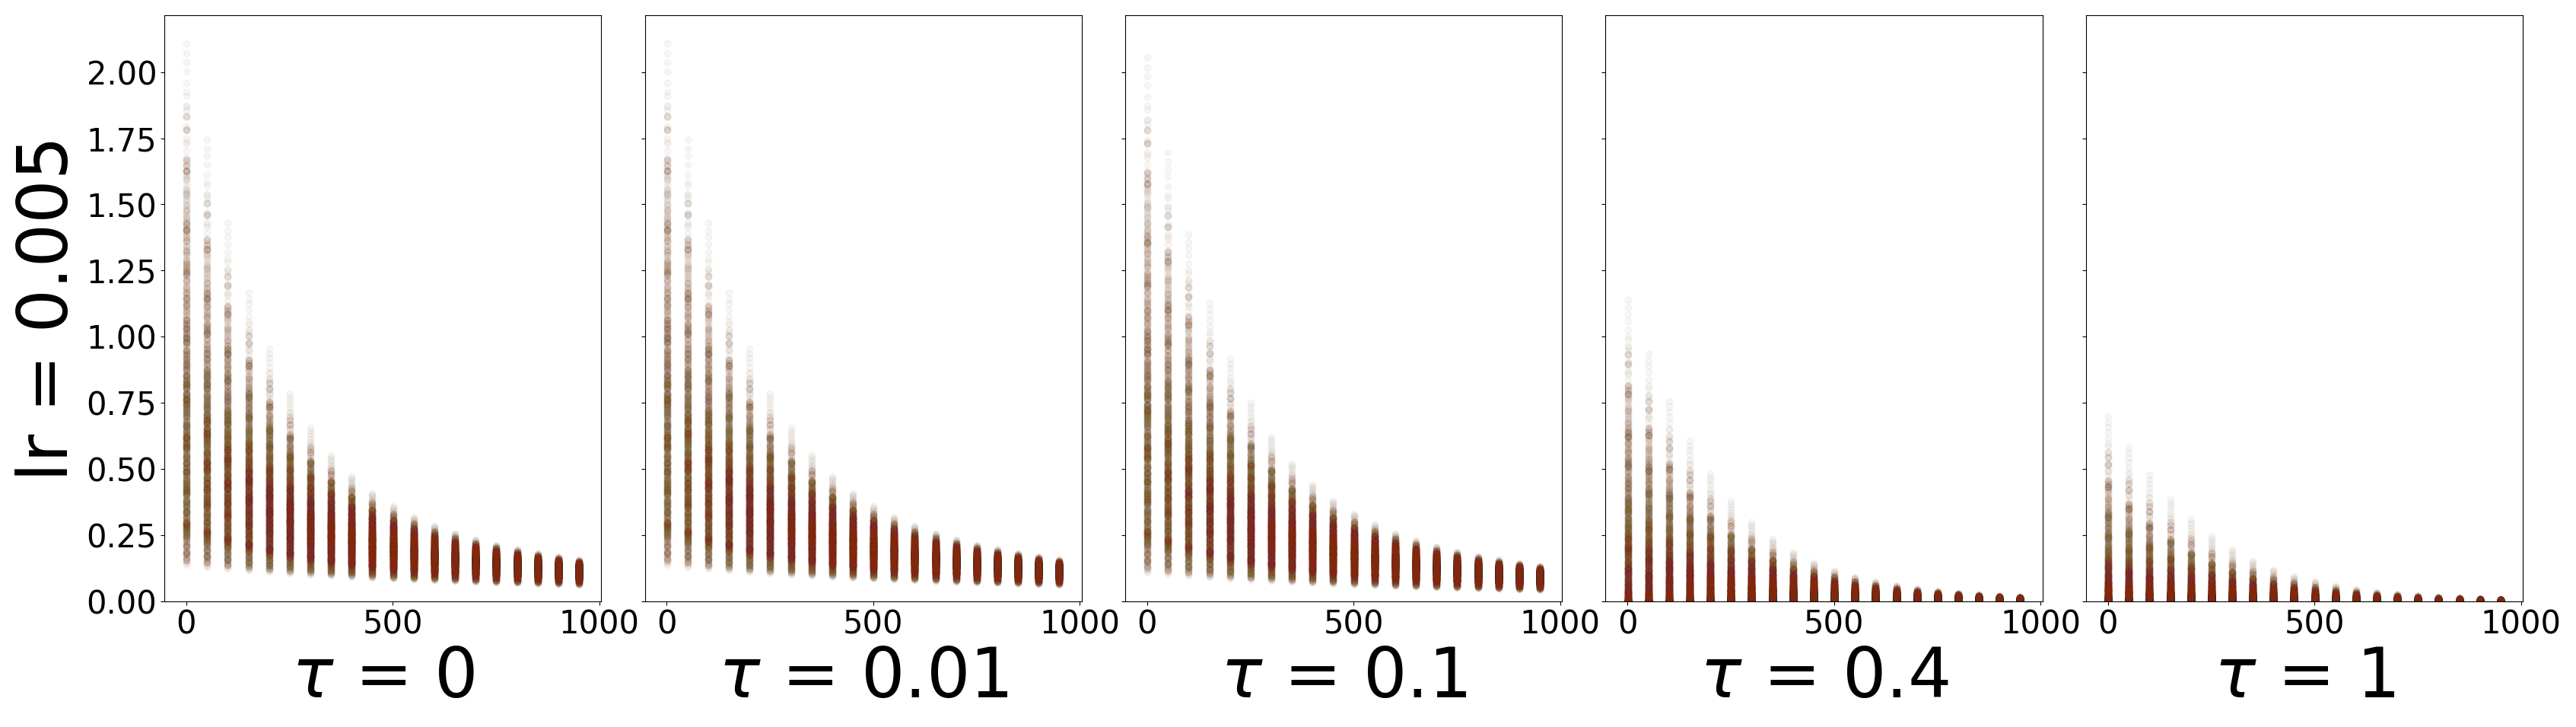
\includegraphics[width=1\columnwidth]{figs/discrete-bandit/notlearnQ/sgd/loss_forward_optim=sgd.png}
% % %     \caption{Forward KL, SGD.}
% % %     \label{fig:discrete-bandit-loss-forward-sgd}
% % %   \end{subfigure}%
% % %   \begin{subfigure}[b]{0.4\linewidth}
% % %     \centering
% % %     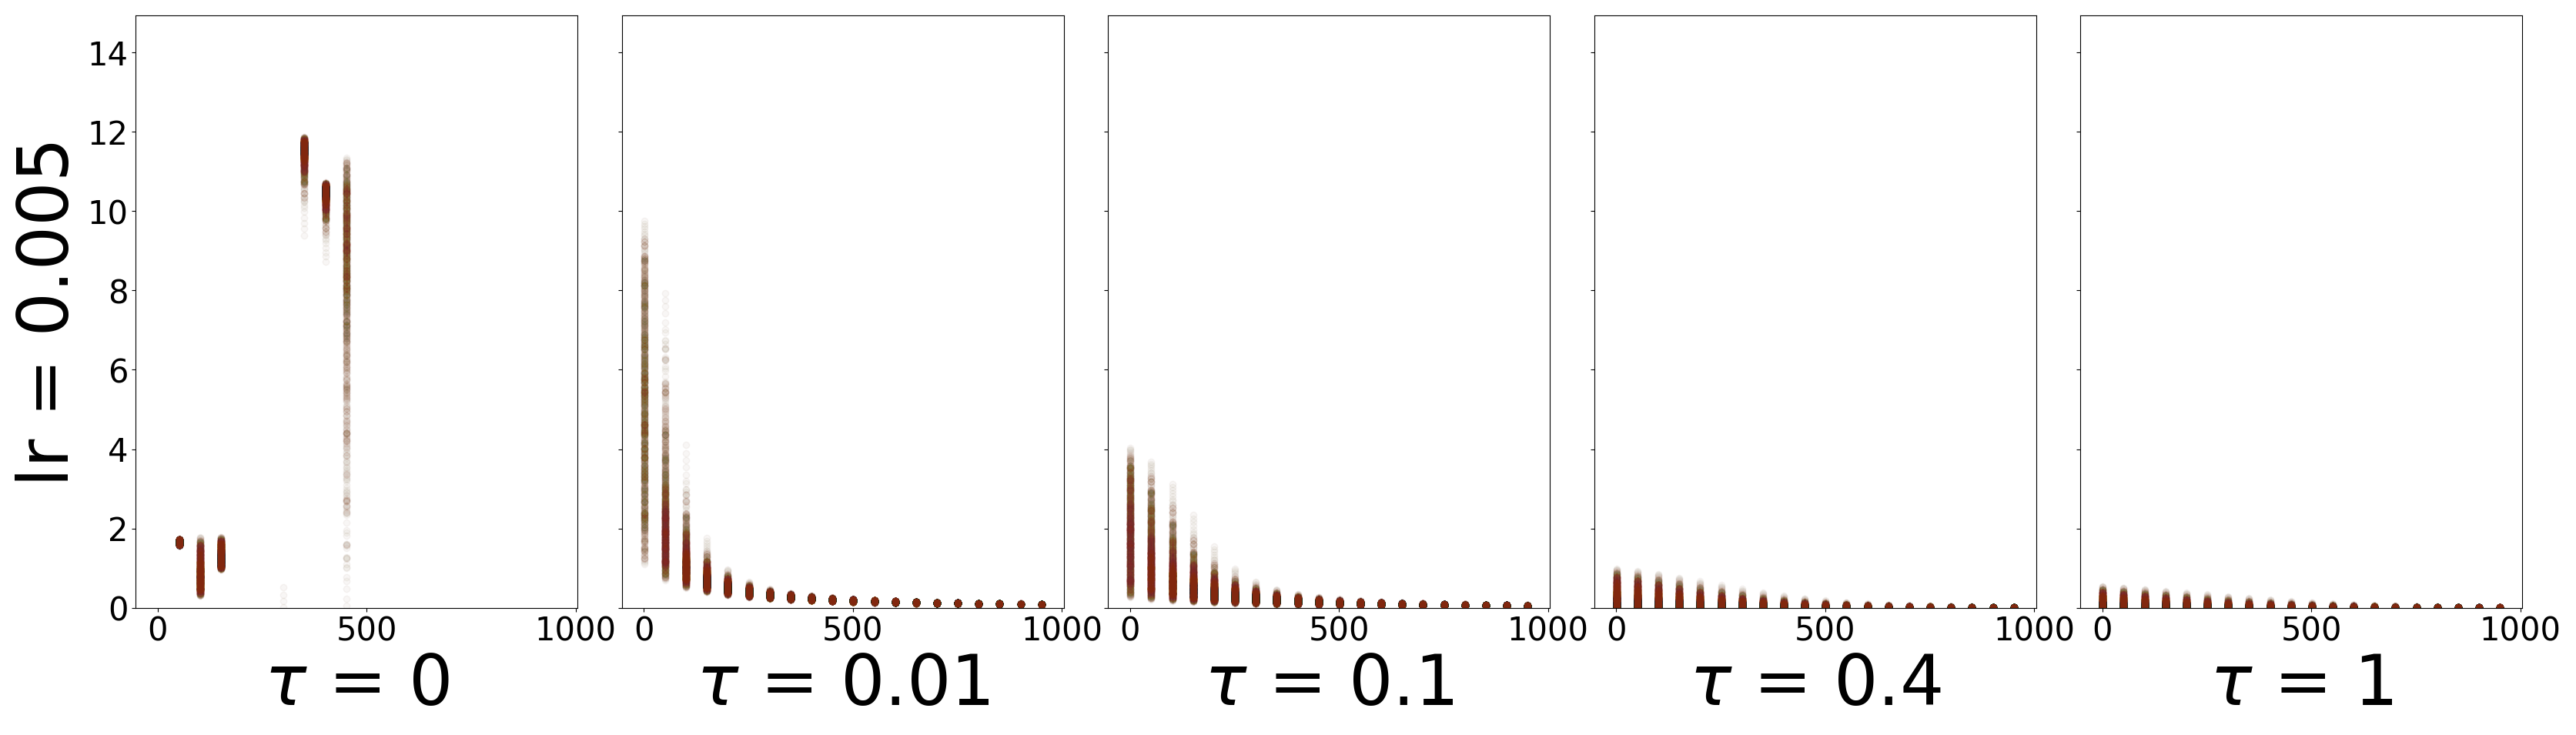
\includegraphics[width=1\columnwidth]{figs/discrete-bandit/notlearnQ/sgd/loss_reverse_optim=sgd.png}
% % %     \caption{Reverse KL, SGD.}
% % %     \label{fig:discrete-bandit-loss-reverse-sgd}
% % %   \end{subfigure}
% % %   \caption{Loss over time with softmax policy. Different colours are different modes. }
% % % \end{figure}

% % \begin{figure}[!ht]
% %   \centering
% %   \begin{subfigure}[b]{0.4\linewidth}
% %     \centering
% %     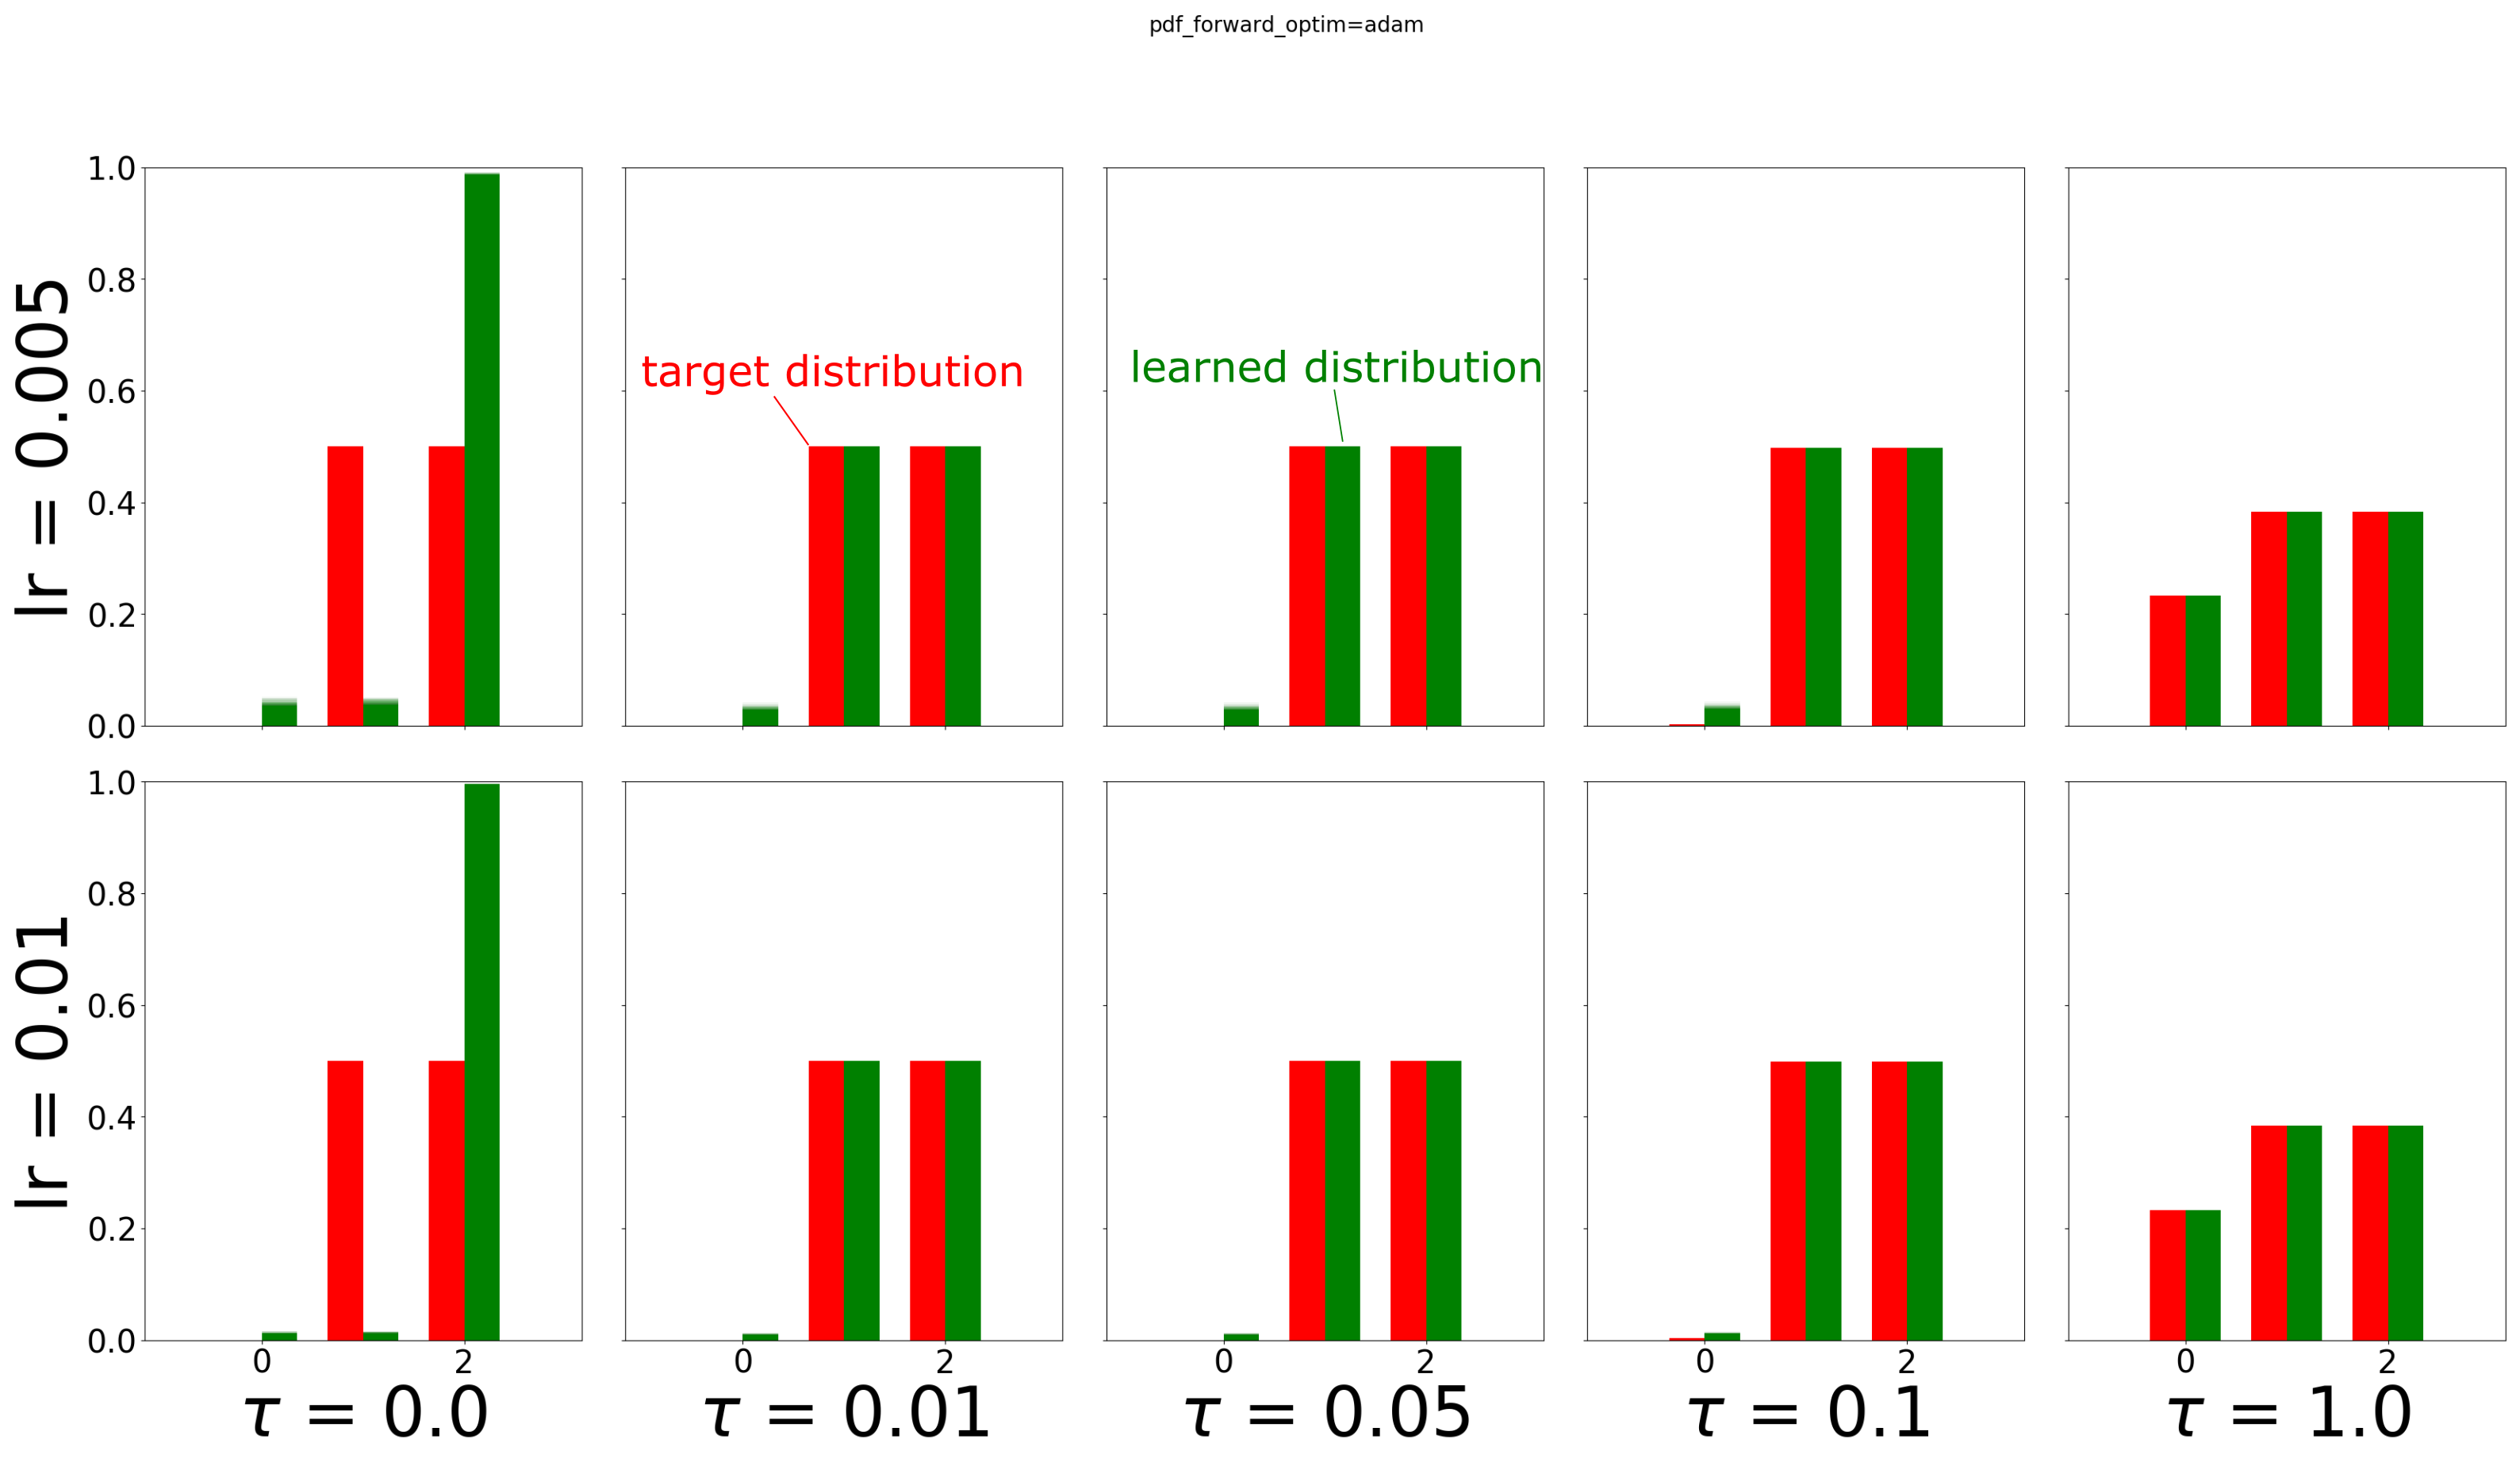
\includegraphics[width=1\columnwidth]{figs/discrete-bandit/notlearnQ/adam/pdf-adam.png}
% %     \caption{Forward KL, Adam.}
% %     \label{fig:discrete-bandit-pdf-forward-adam}
% %   \end{subfigure}%
% %   \begin{subfigure}[b]{0.4\linewidth}
% %     \centering
% %     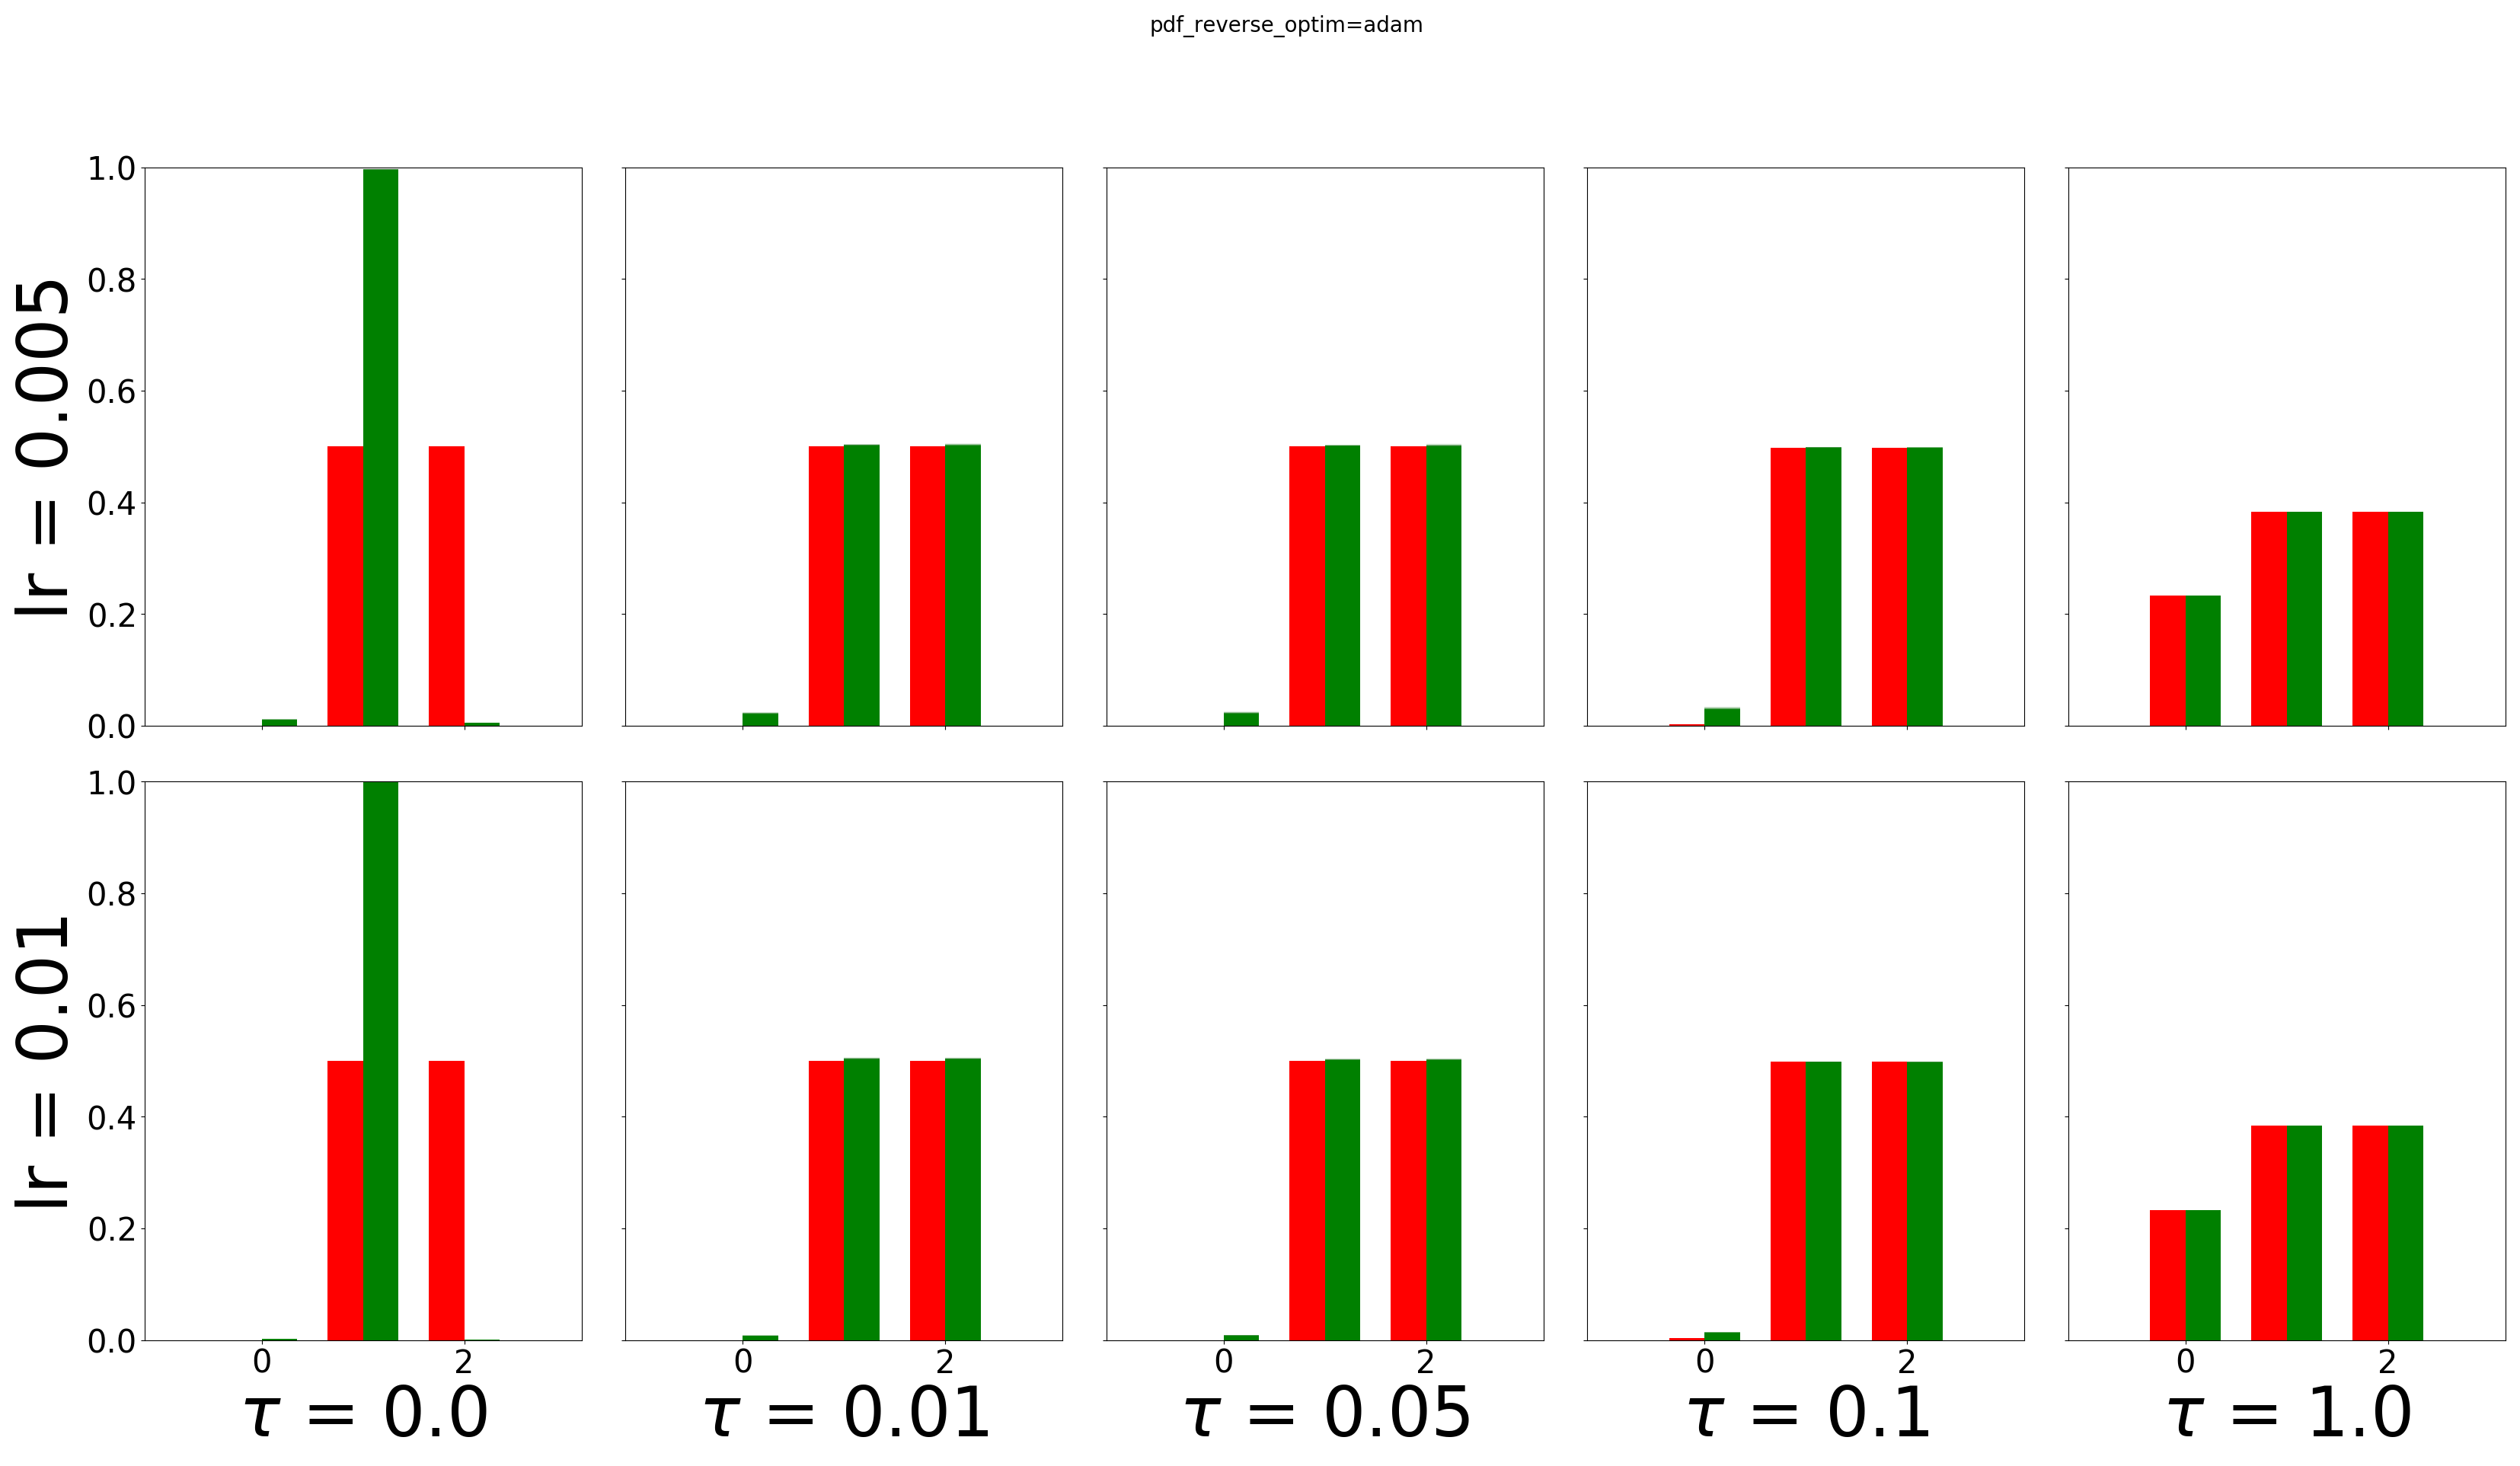
\includegraphics[width=1\columnwidth]{figs/discrete-bandit/notlearnQ/adam/pdf_reverse_optim=adam.png}
% %     \caption{Reverse KL, Adam. }
% %     \label{fig:discrete-bandit-pdf-reverse-adam}
% %   \end{subfigure}
  
% %   \begin{subfigure}[b]{0.4\linewidth}
% %     \centering
% %     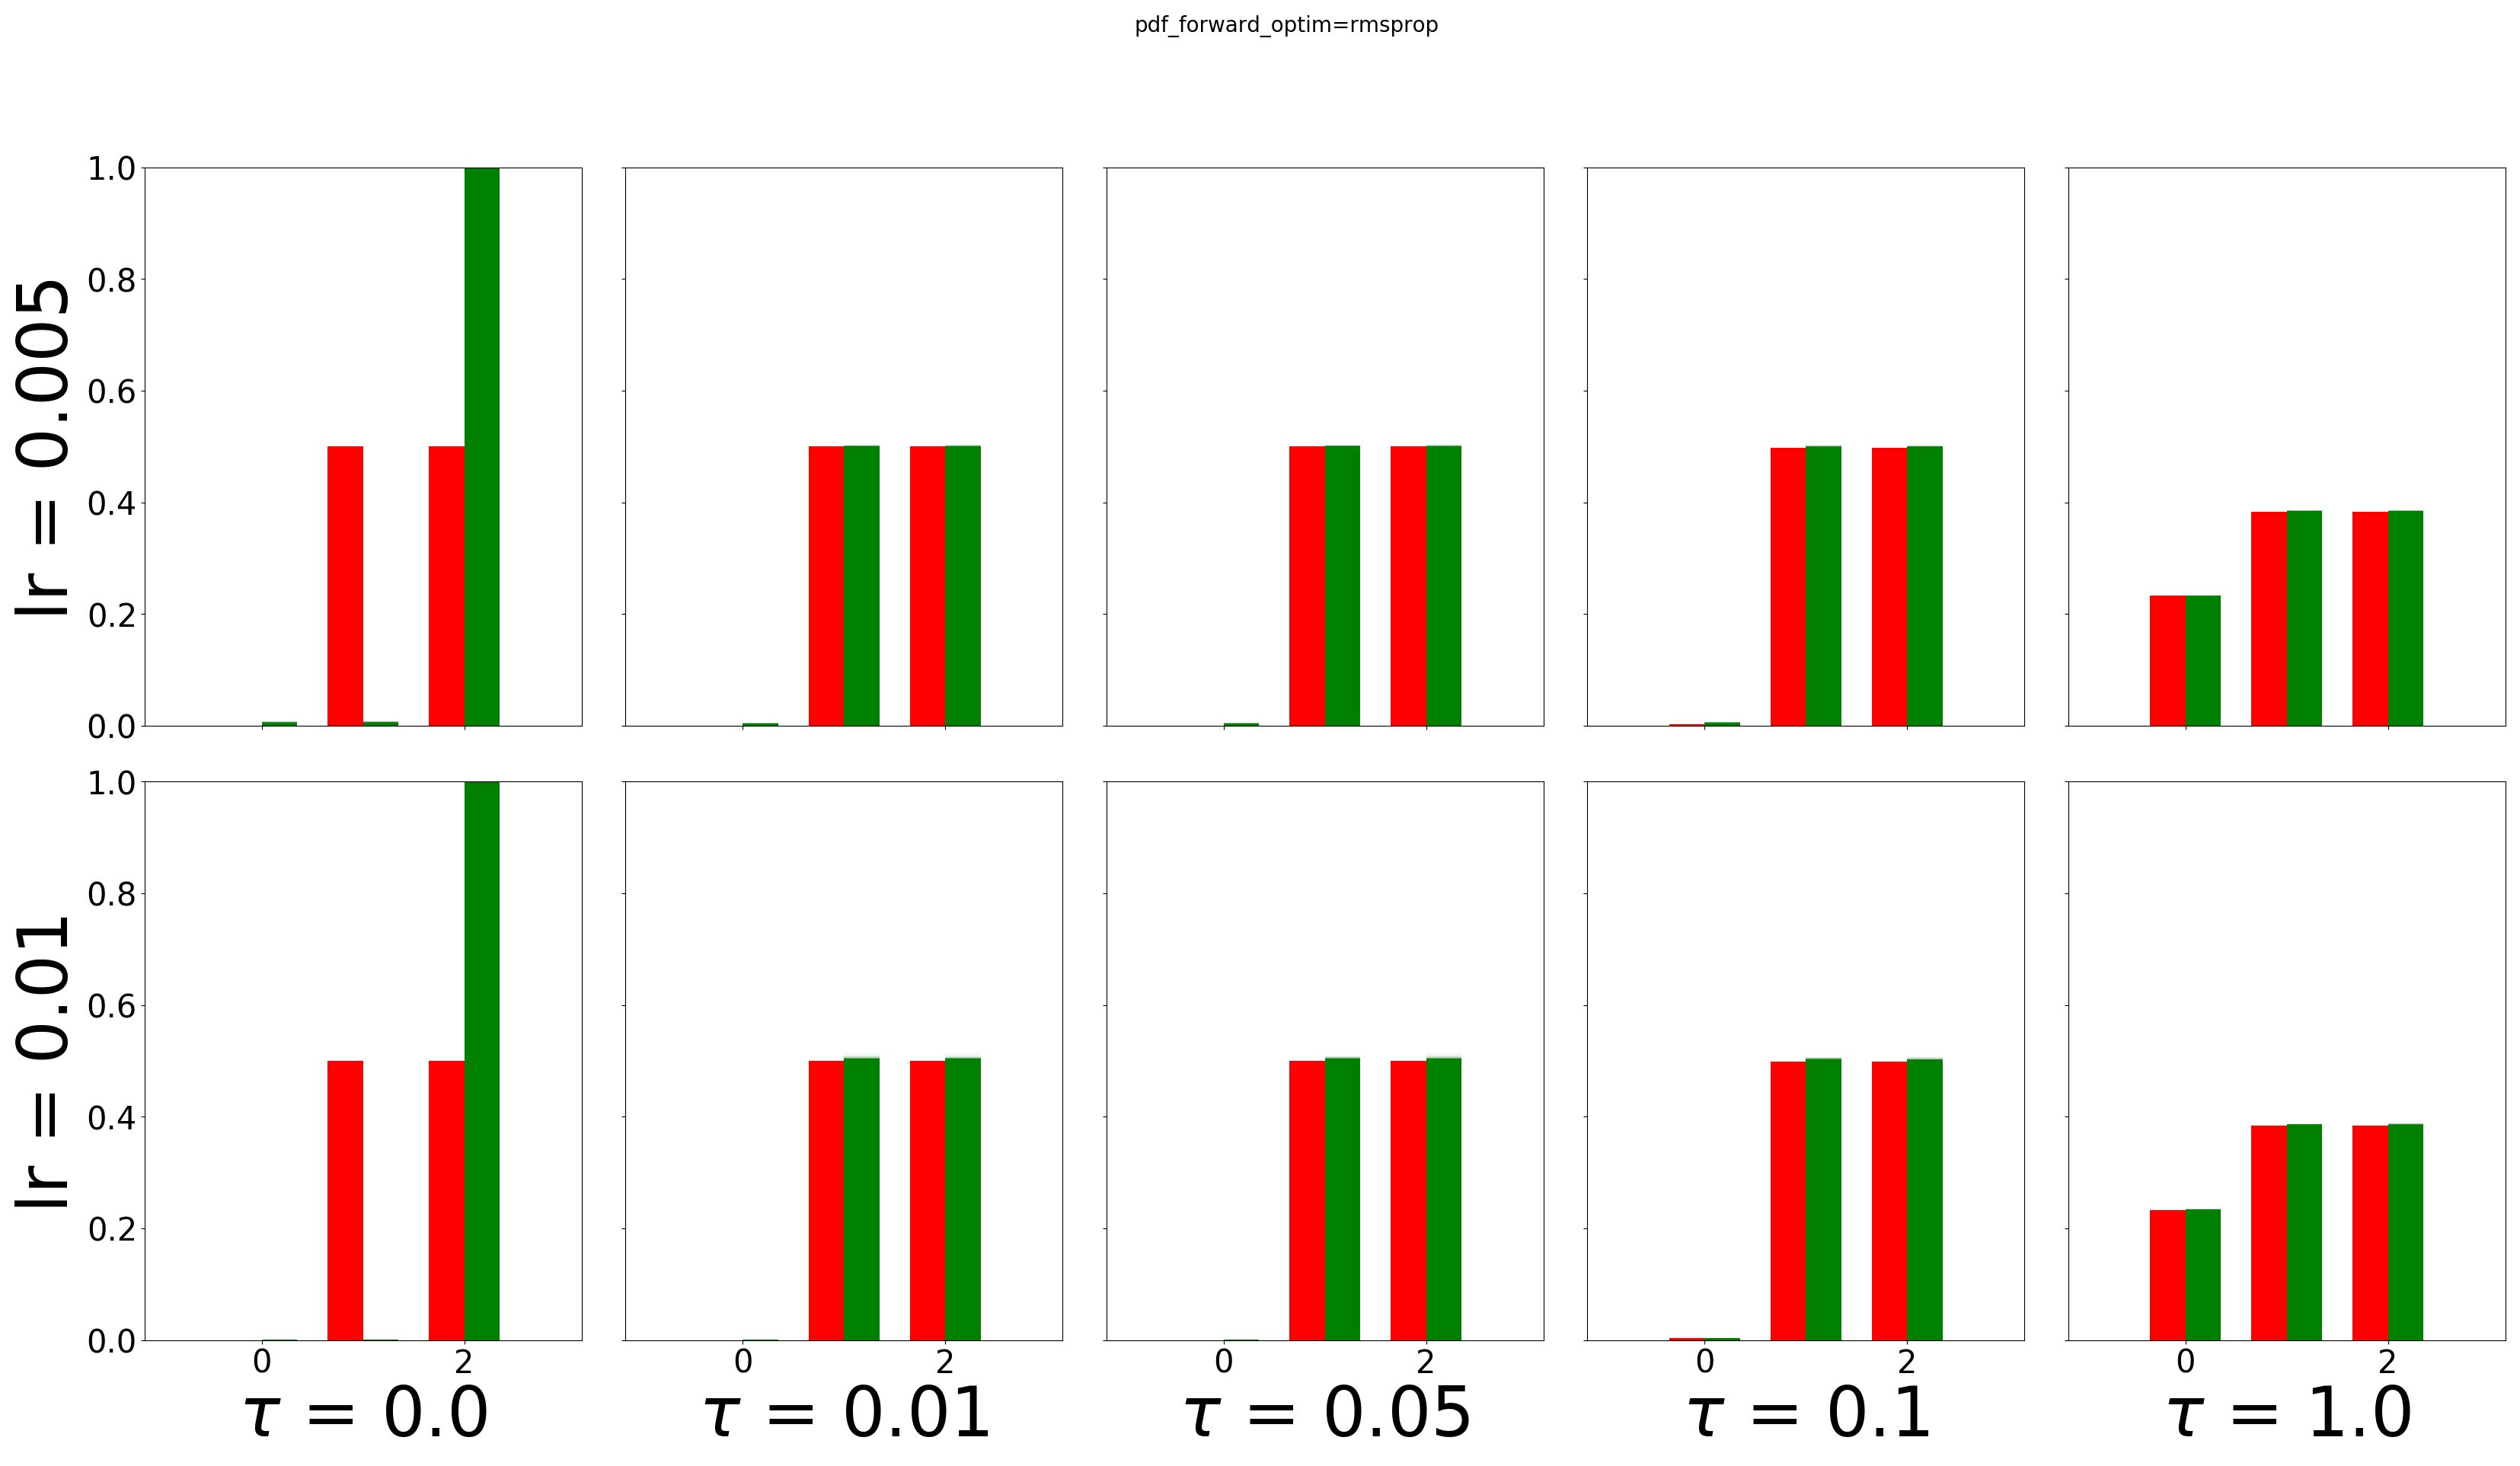
\includegraphics[width=1\columnwidth]{figs/discrete-bandit/notlearnQ/rmsprop/pdf_forward_optim=rmsprop.png}
% %     \caption{Forward KL, RMSprop.}
% %     \label{fig:discrete-bandit-pdf-forward-rmsprop}
% %   \end{subfigure}%
% %   \begin{subfigure}[b]{0.4\linewidth}
% %     \centering
% %     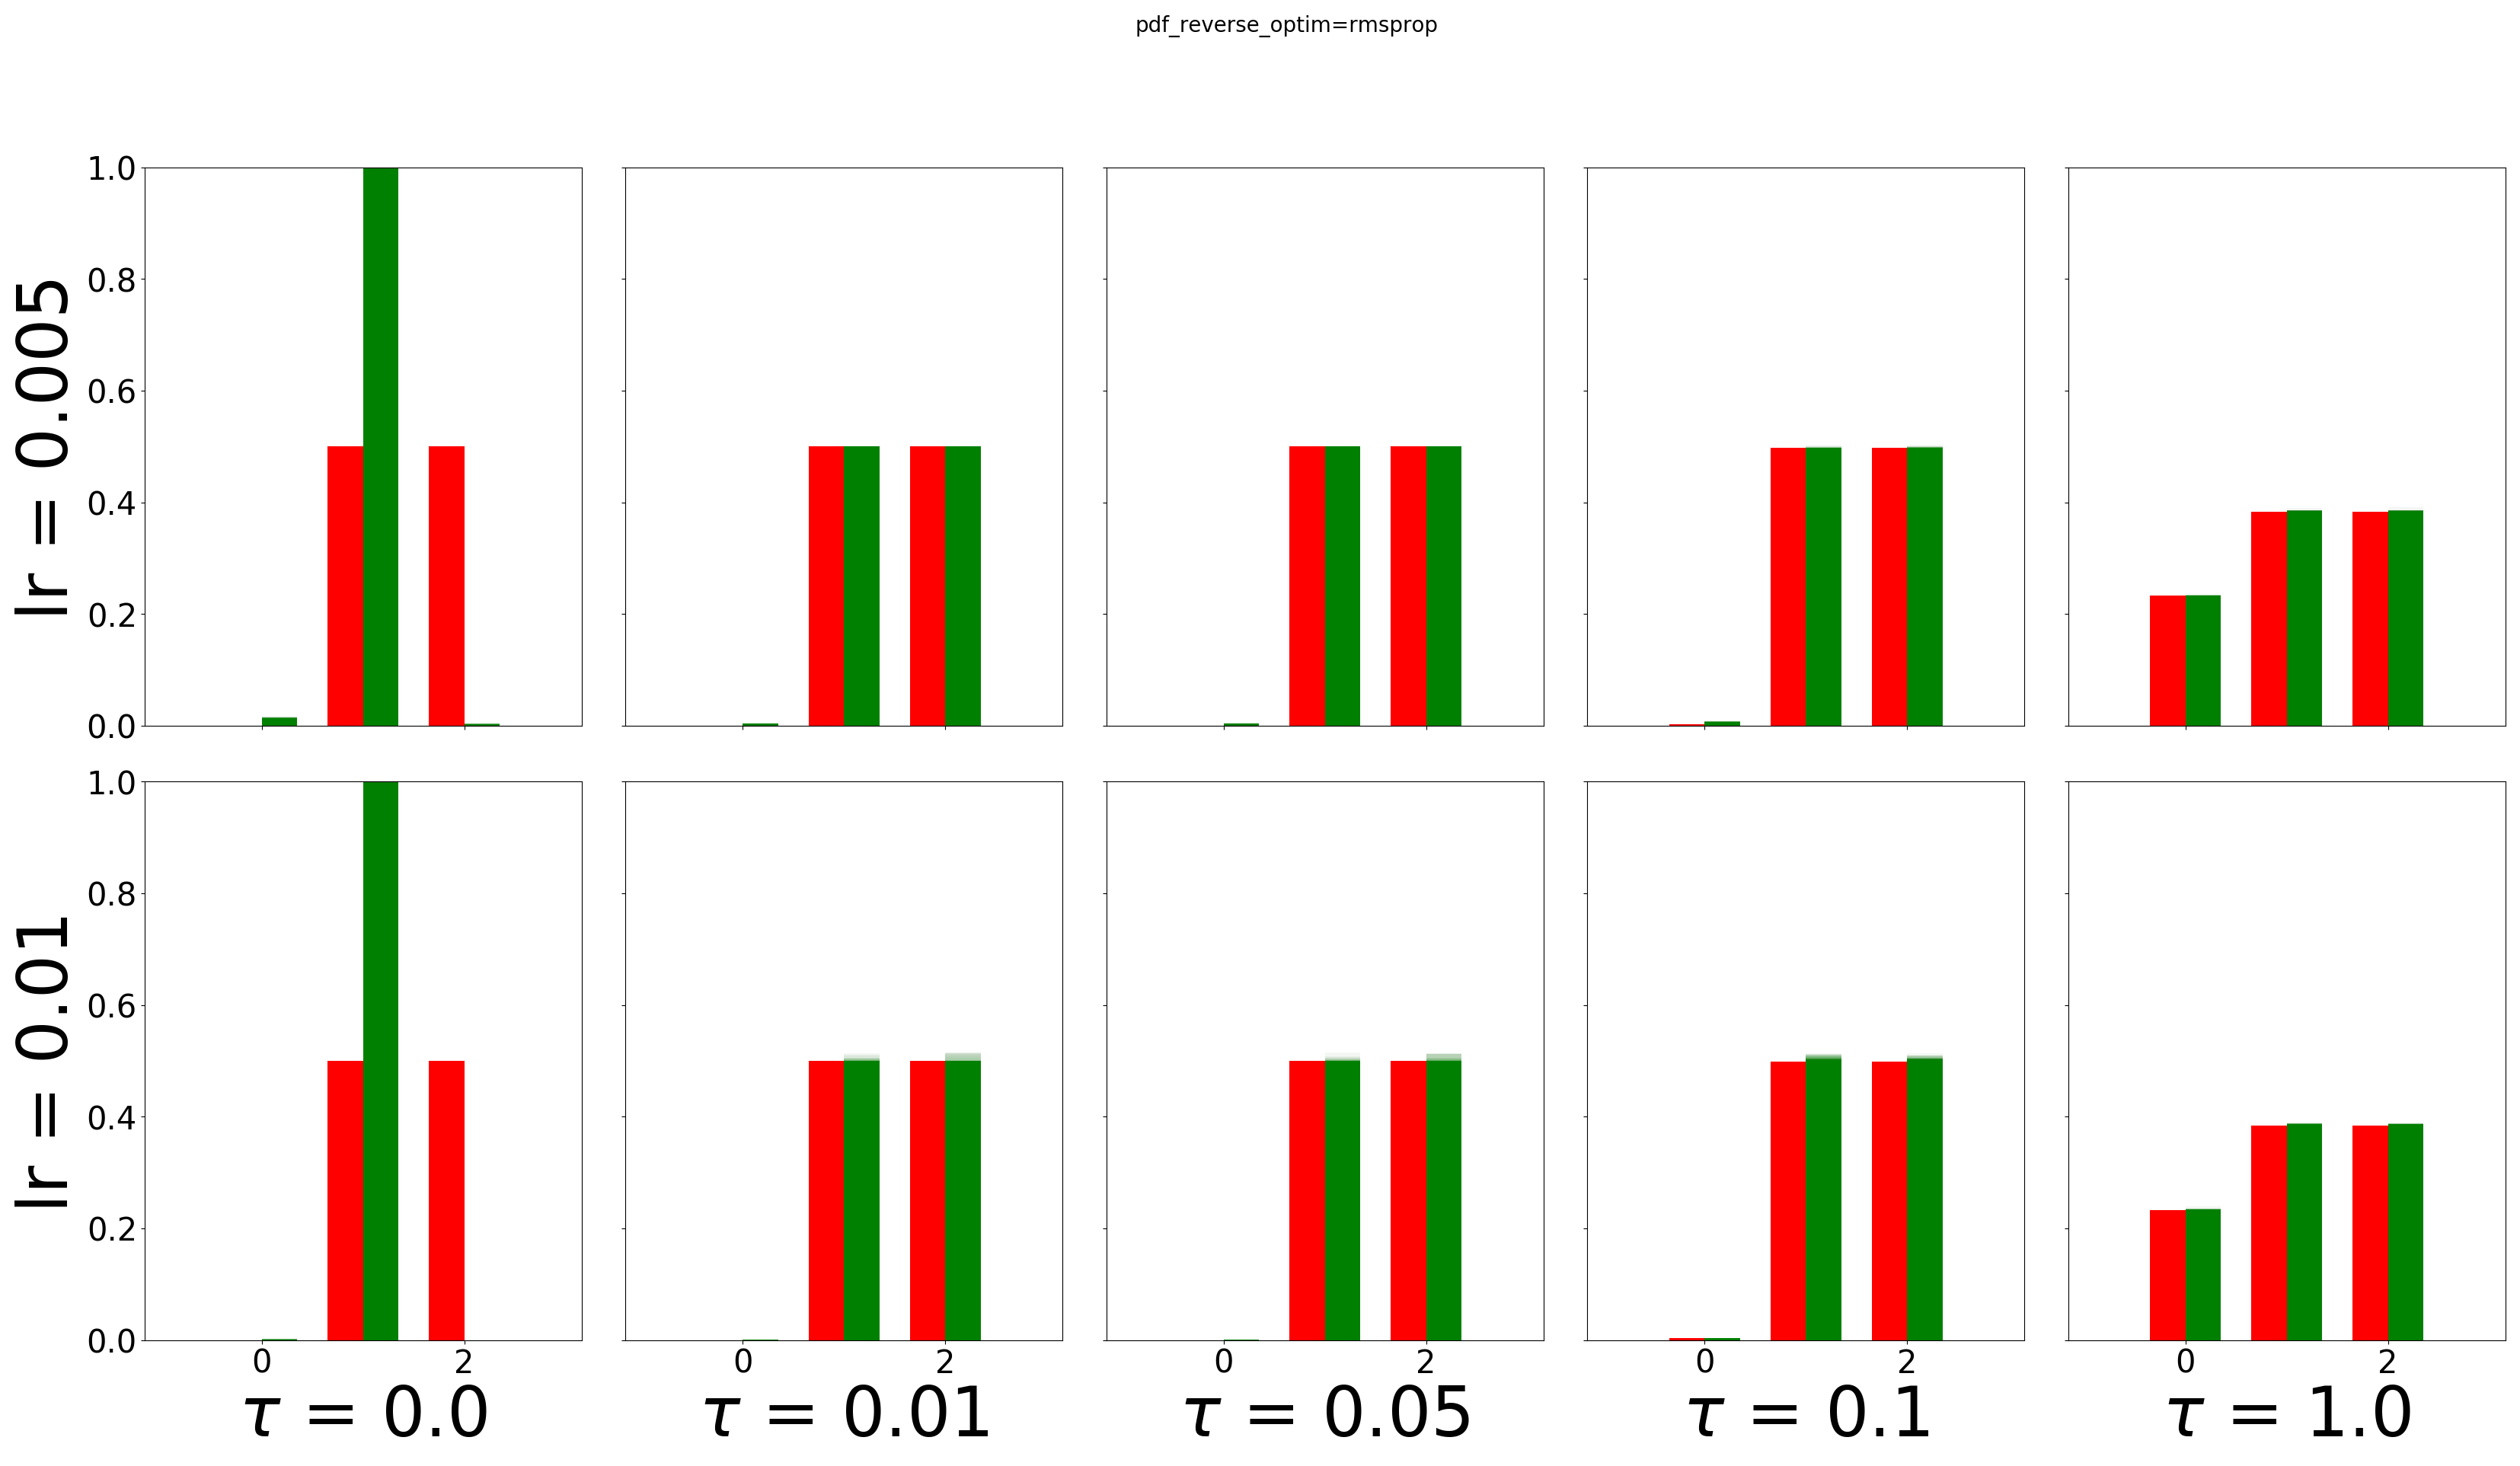
\includegraphics[width=1\columnwidth]{figs/discrete-bandit/notlearnQ/rmsprop/pdf_reverse_optim=rmsprop.png}
% %     \caption{Reverse KL, RMSprop.}
% %     \label{fig:discrete-bandit-pdf-reverse-rmsprop}
% %   \end{subfigure}
  
% %   \begin{subfigure}[b]{0.4\linewidth}
% %     \centering
% %     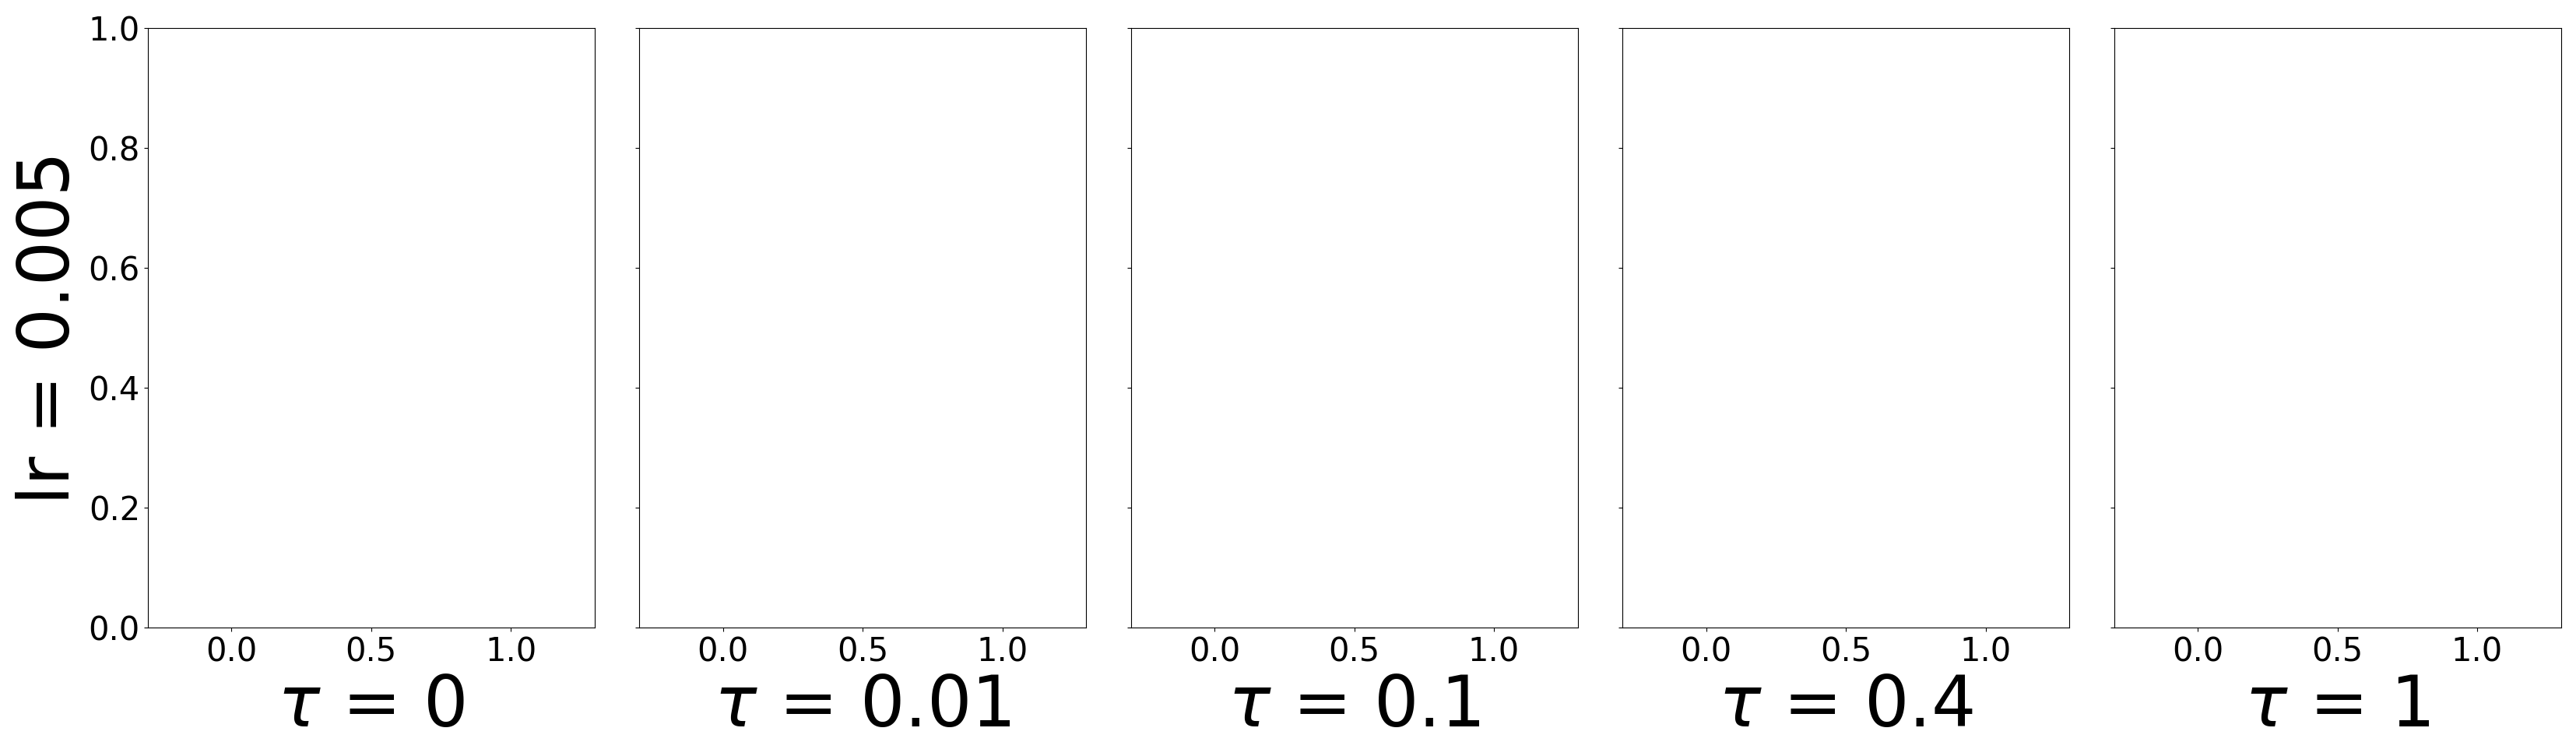
\includegraphics[width=1\columnwidth]{figs/discrete-bandit/notlearnQ/sgd/pdf_forward_optim=sgd.png}
% %     \caption{Forward KL, SGD.}
% %     \label{fig:discrete-bandit-pdf-forward-sgd}
% %   \end{subfigure}%
% %   \begin{subfigure}[b]{0.4\linewidth}
% %     \centering
% %     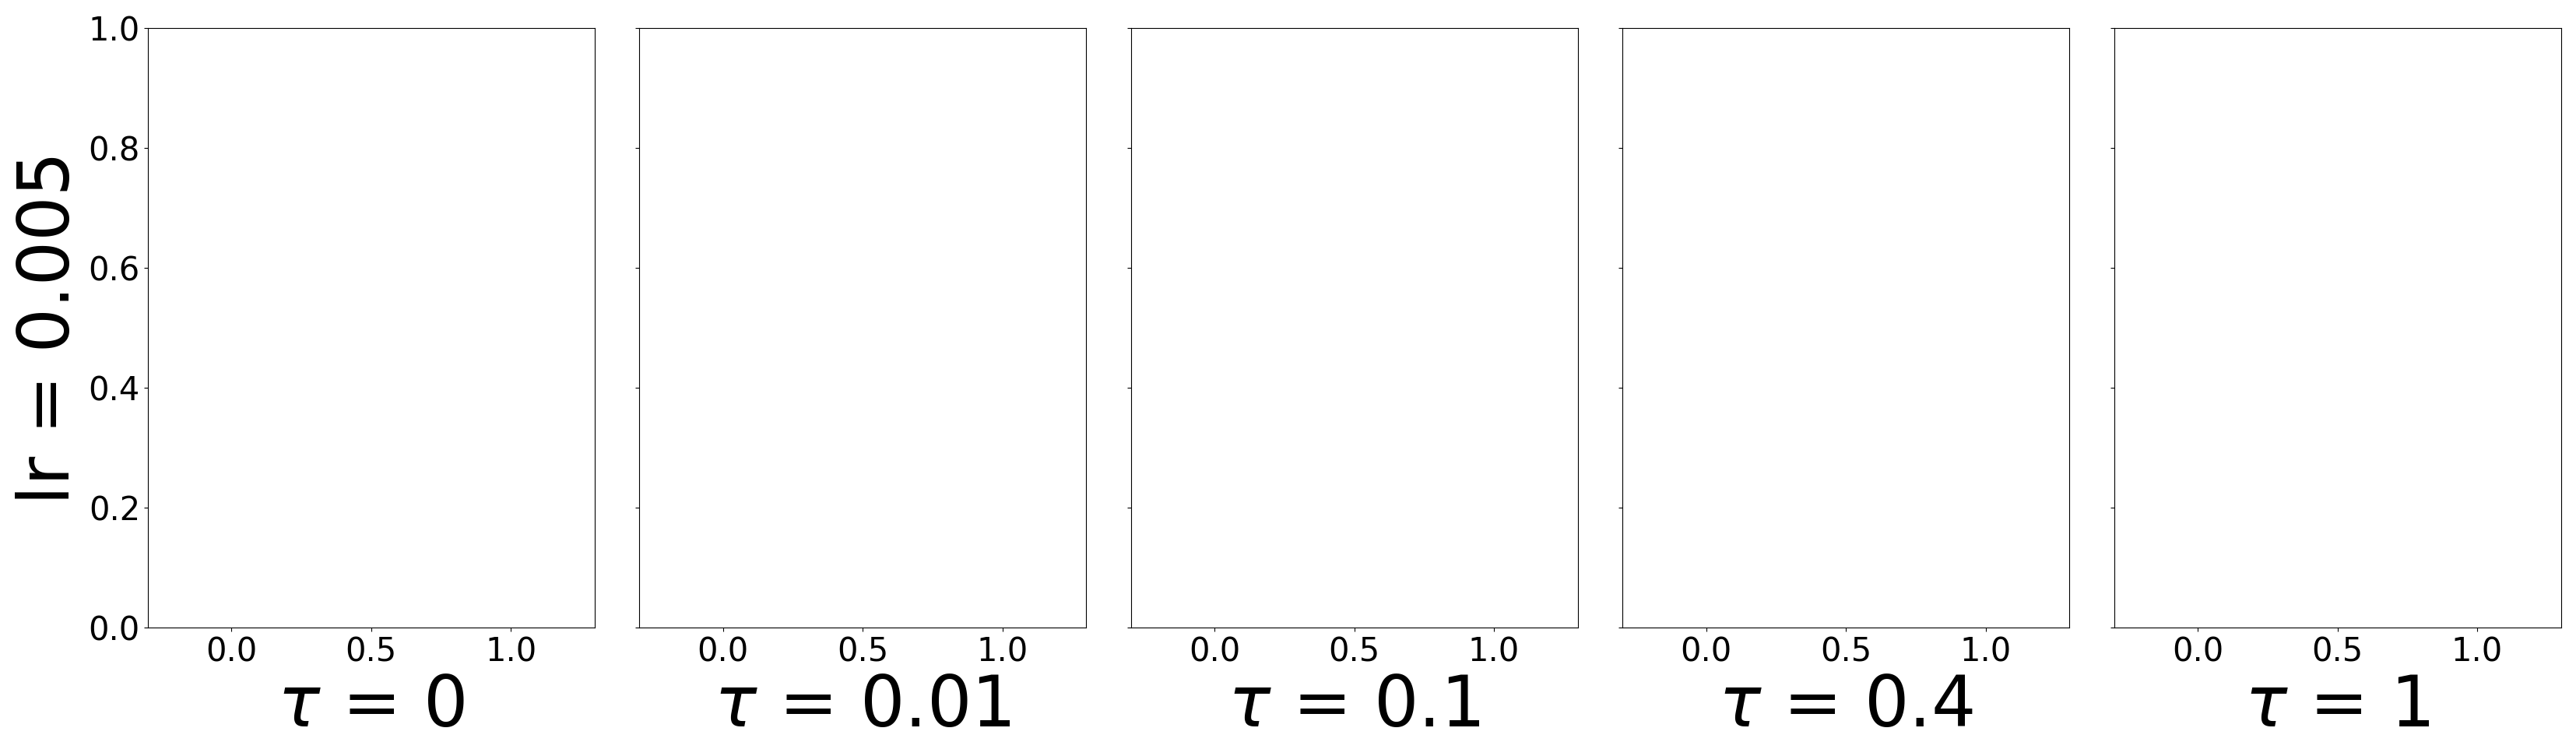
\includegraphics[width=1\columnwidth]{figs/discrete-bandit/notlearnQ/sgd/pdf_reverse_optim=sgd.png}
% %     \caption{Reverse KL, SGD.}
% %     \label{fig:discrete-bandit-pdf-reverse-sgd}
% %   \end{subfigure}
% %   \caption{Final PDF with softmax policy. Red is the target PDF and green is the policy PDF. }
% % \end{figure}


% \clearpage

% \subsection{Switch-Stay}\label{sec:switch-stay}
% We include plots for other optimizers.
% \textbf{Continuous Switch-Stay}
% \begin{figure}[!htb]
%   \centering
%   \begin{subfigure}[b]{0.5\linewidth}
%     \centering
%     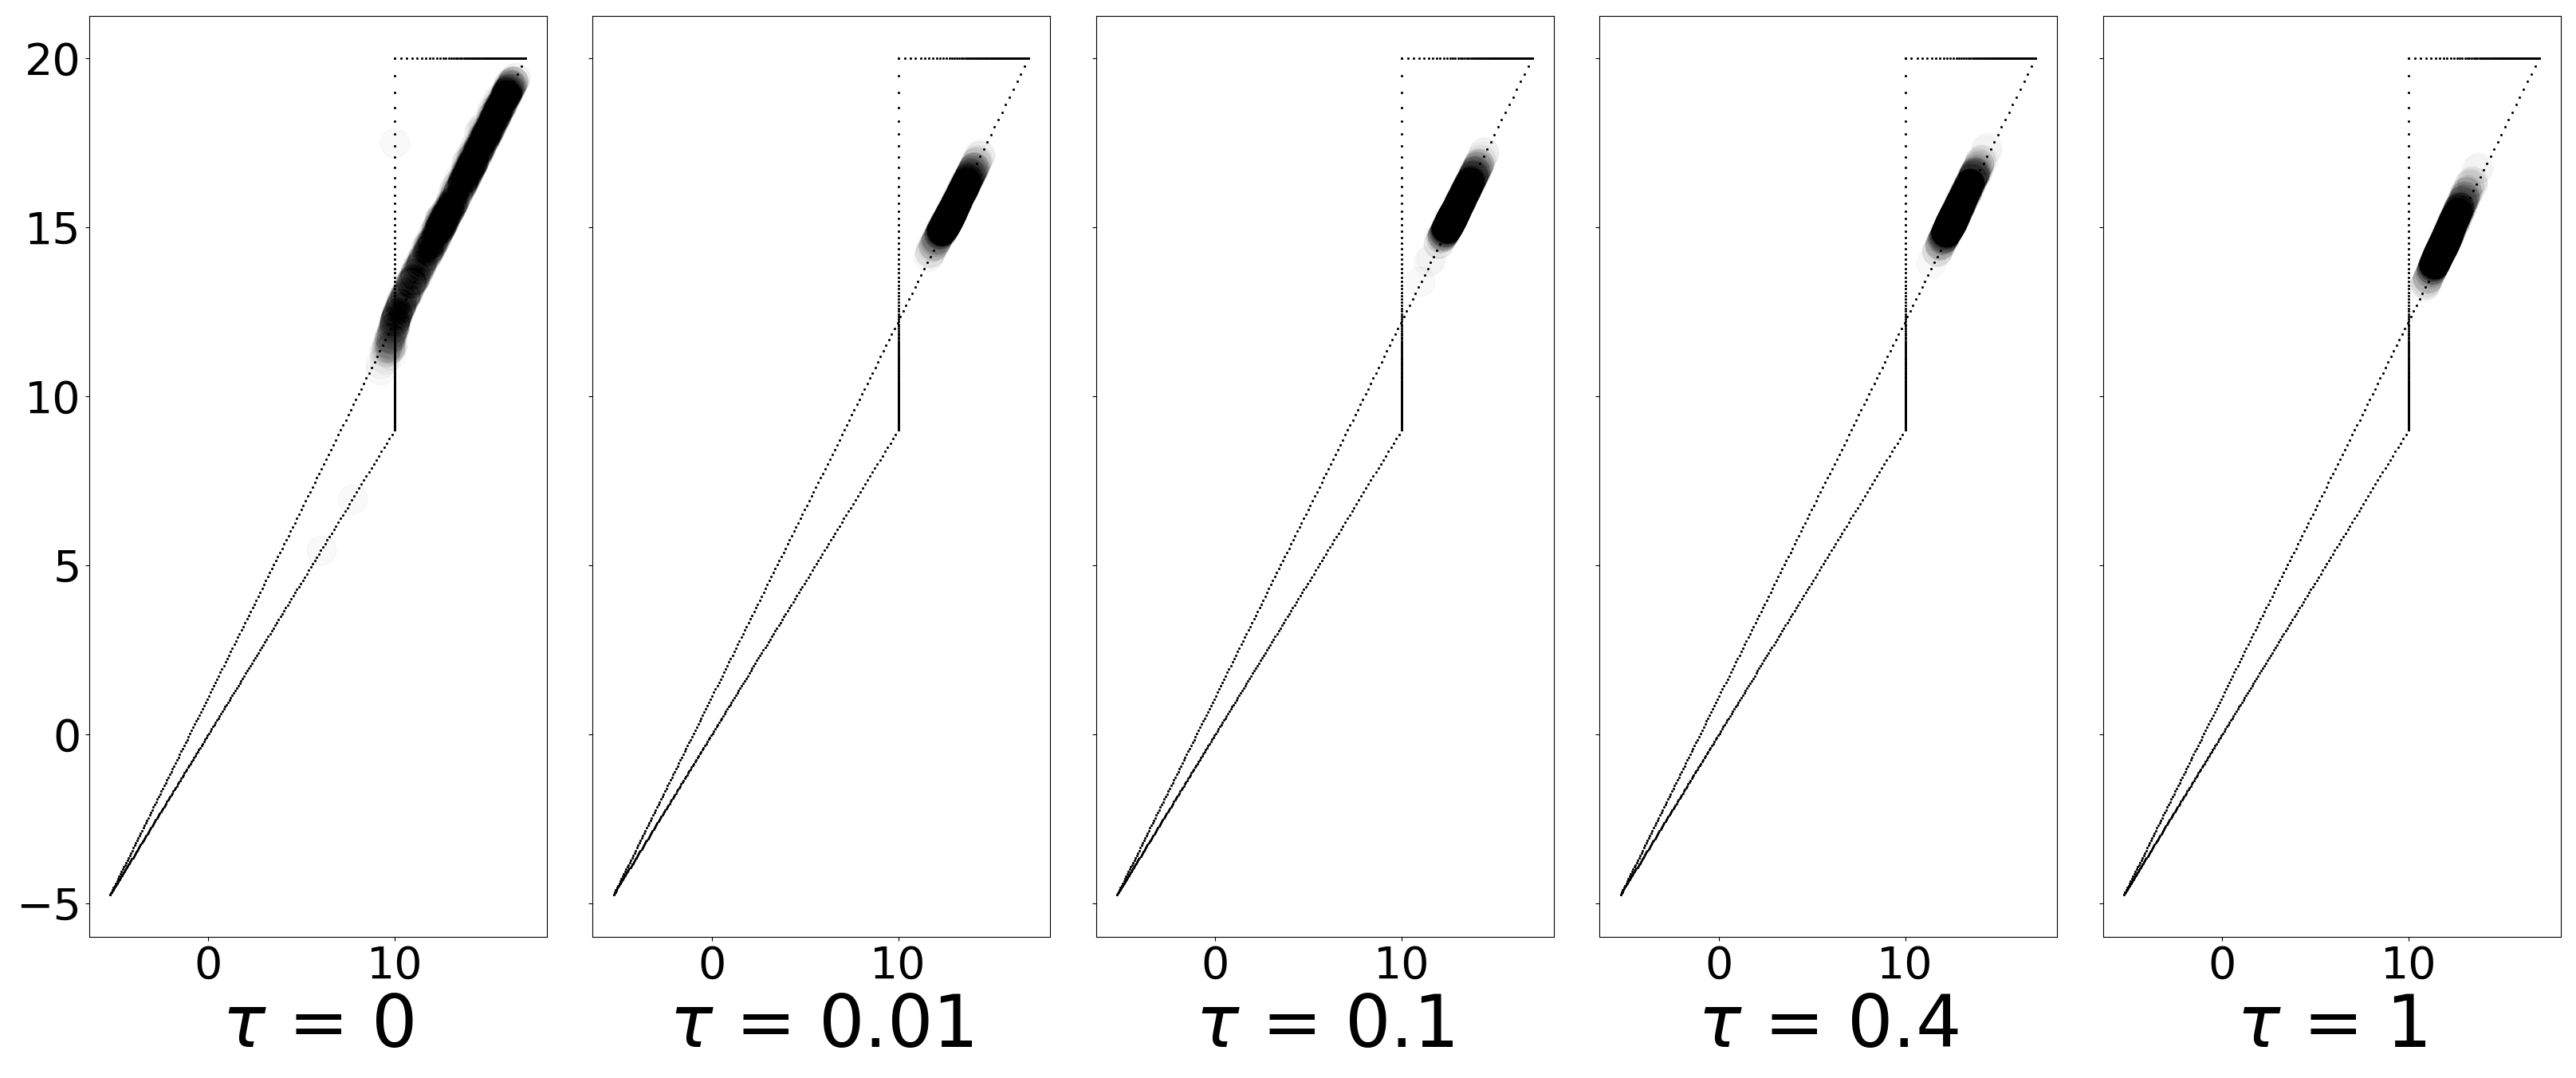
\includegraphics[width=0.8\columnwidth]{figs/continuous-switch-stay/notlearnQ/polytope_forward_optim=rmsprop_lr=0.005.png}
%     \caption{Forward KL.}
%     \label{fig:cont-switch-stay-forward-rmsprop}
%   \end{subfigure}%
%   \begin{subfigure}[b]{0.5\linewidth}
%         \centering
%         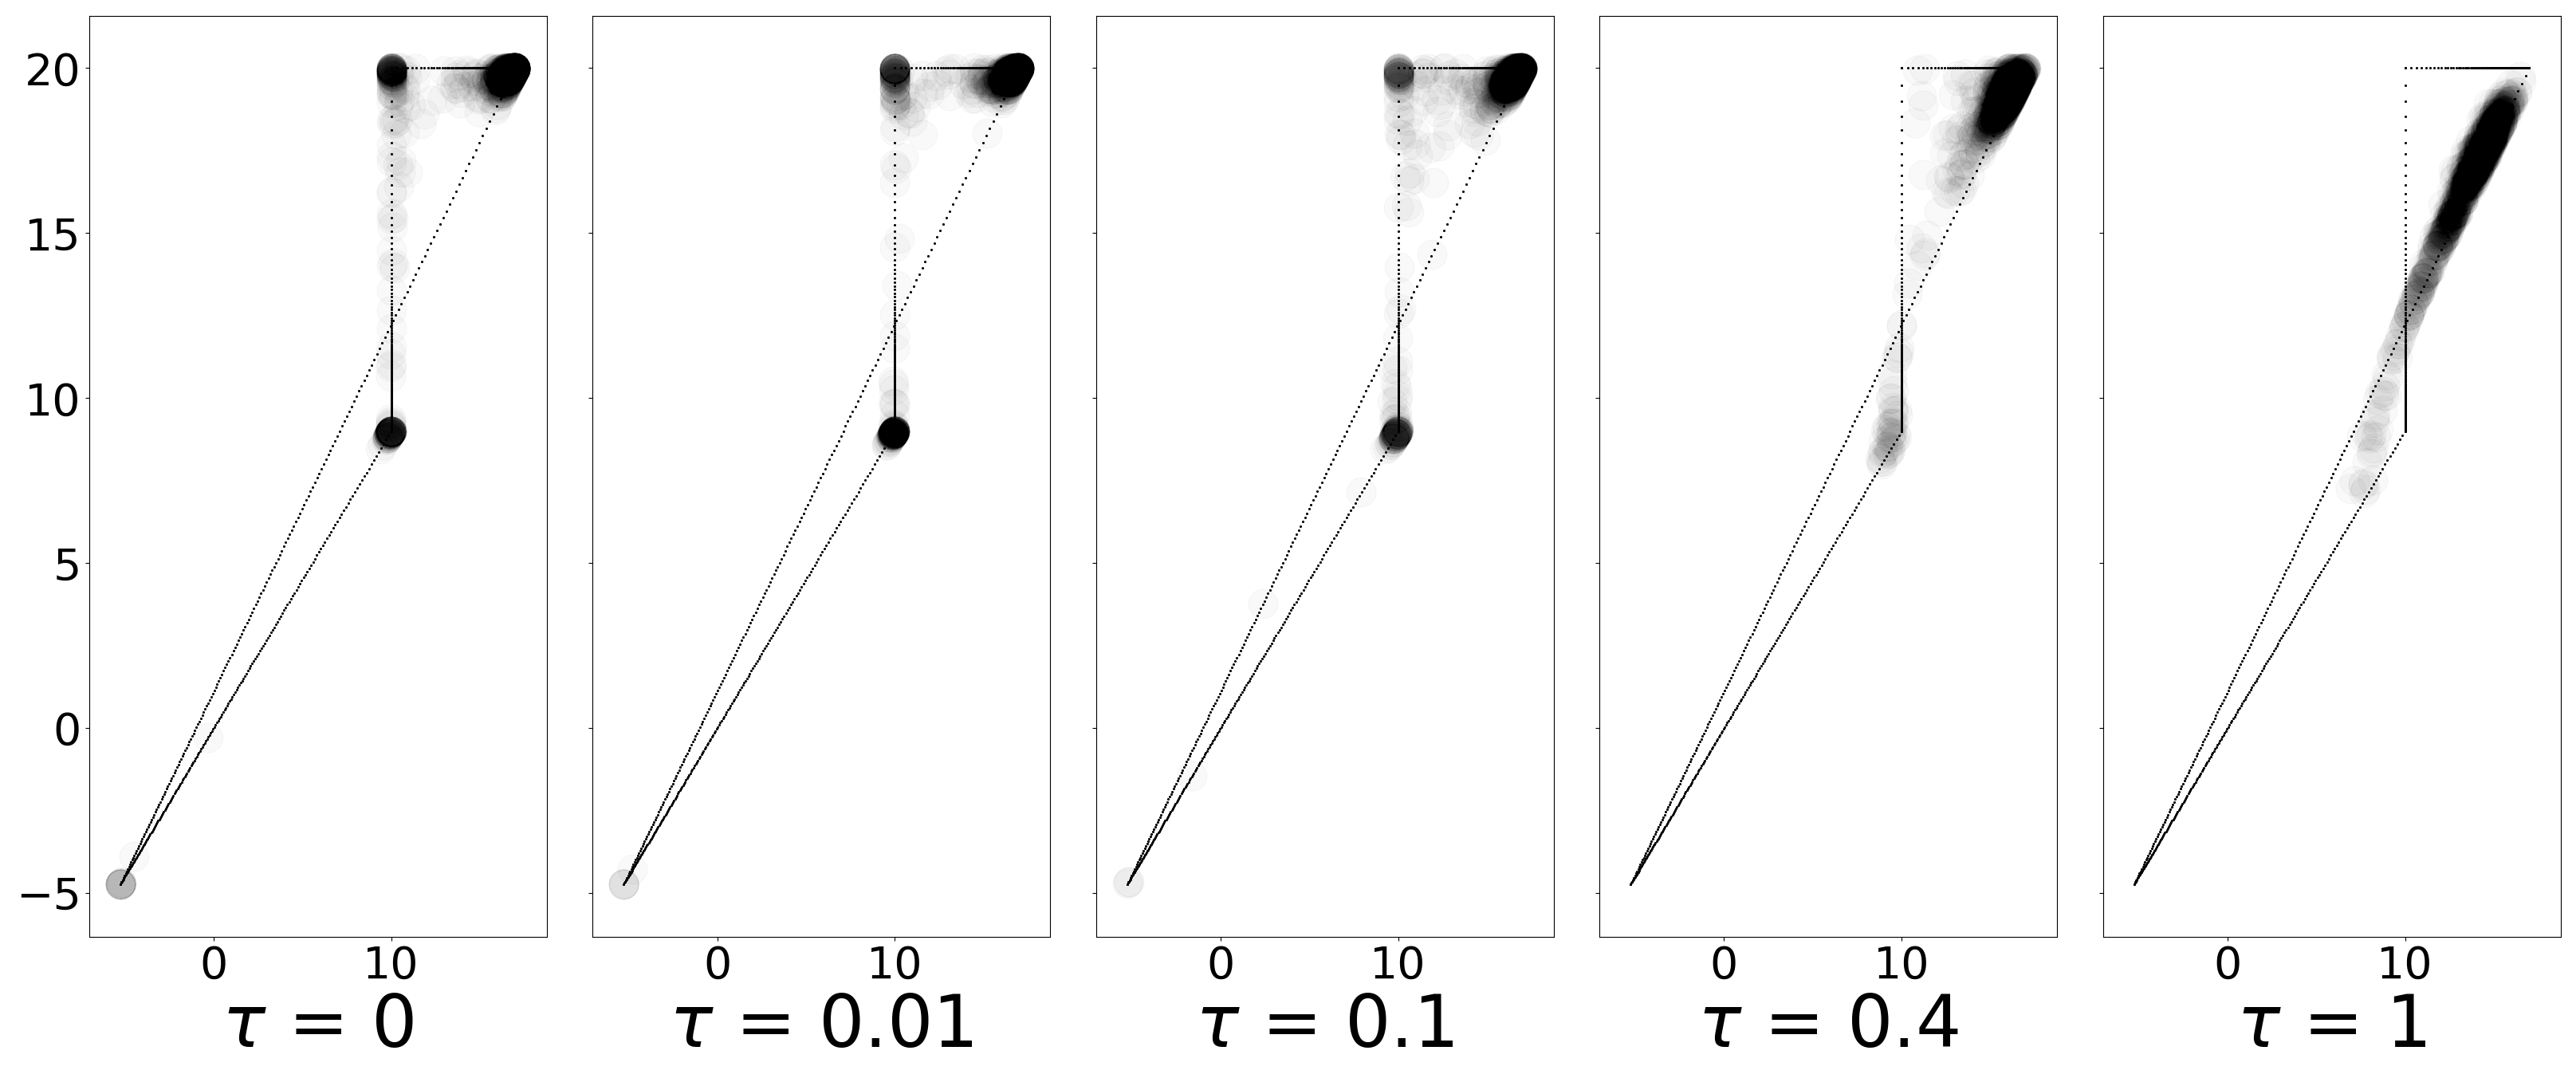
\includegraphics[width=0.8\columnwidth]{figs/continuous-switch-stay/notlearnQ/polytope_reverse_optim=rmsprop_lr=0.005.png}
%         \caption{Reverse KL.}
%         \label{fig:cont-switch-stay-reverse-rmsprop}
%   \end{subfigure}
%   \caption{Final value functions on continuous version of switch-stay after 500 gradient steps, $\gamma = 0.9$. Using RMSprop.}
% \end{figure}

% \begin{figure}[!htb]
%   \centering
%   \begin{subfigure}[b]{0.5\linewidth}
%     \centering
%     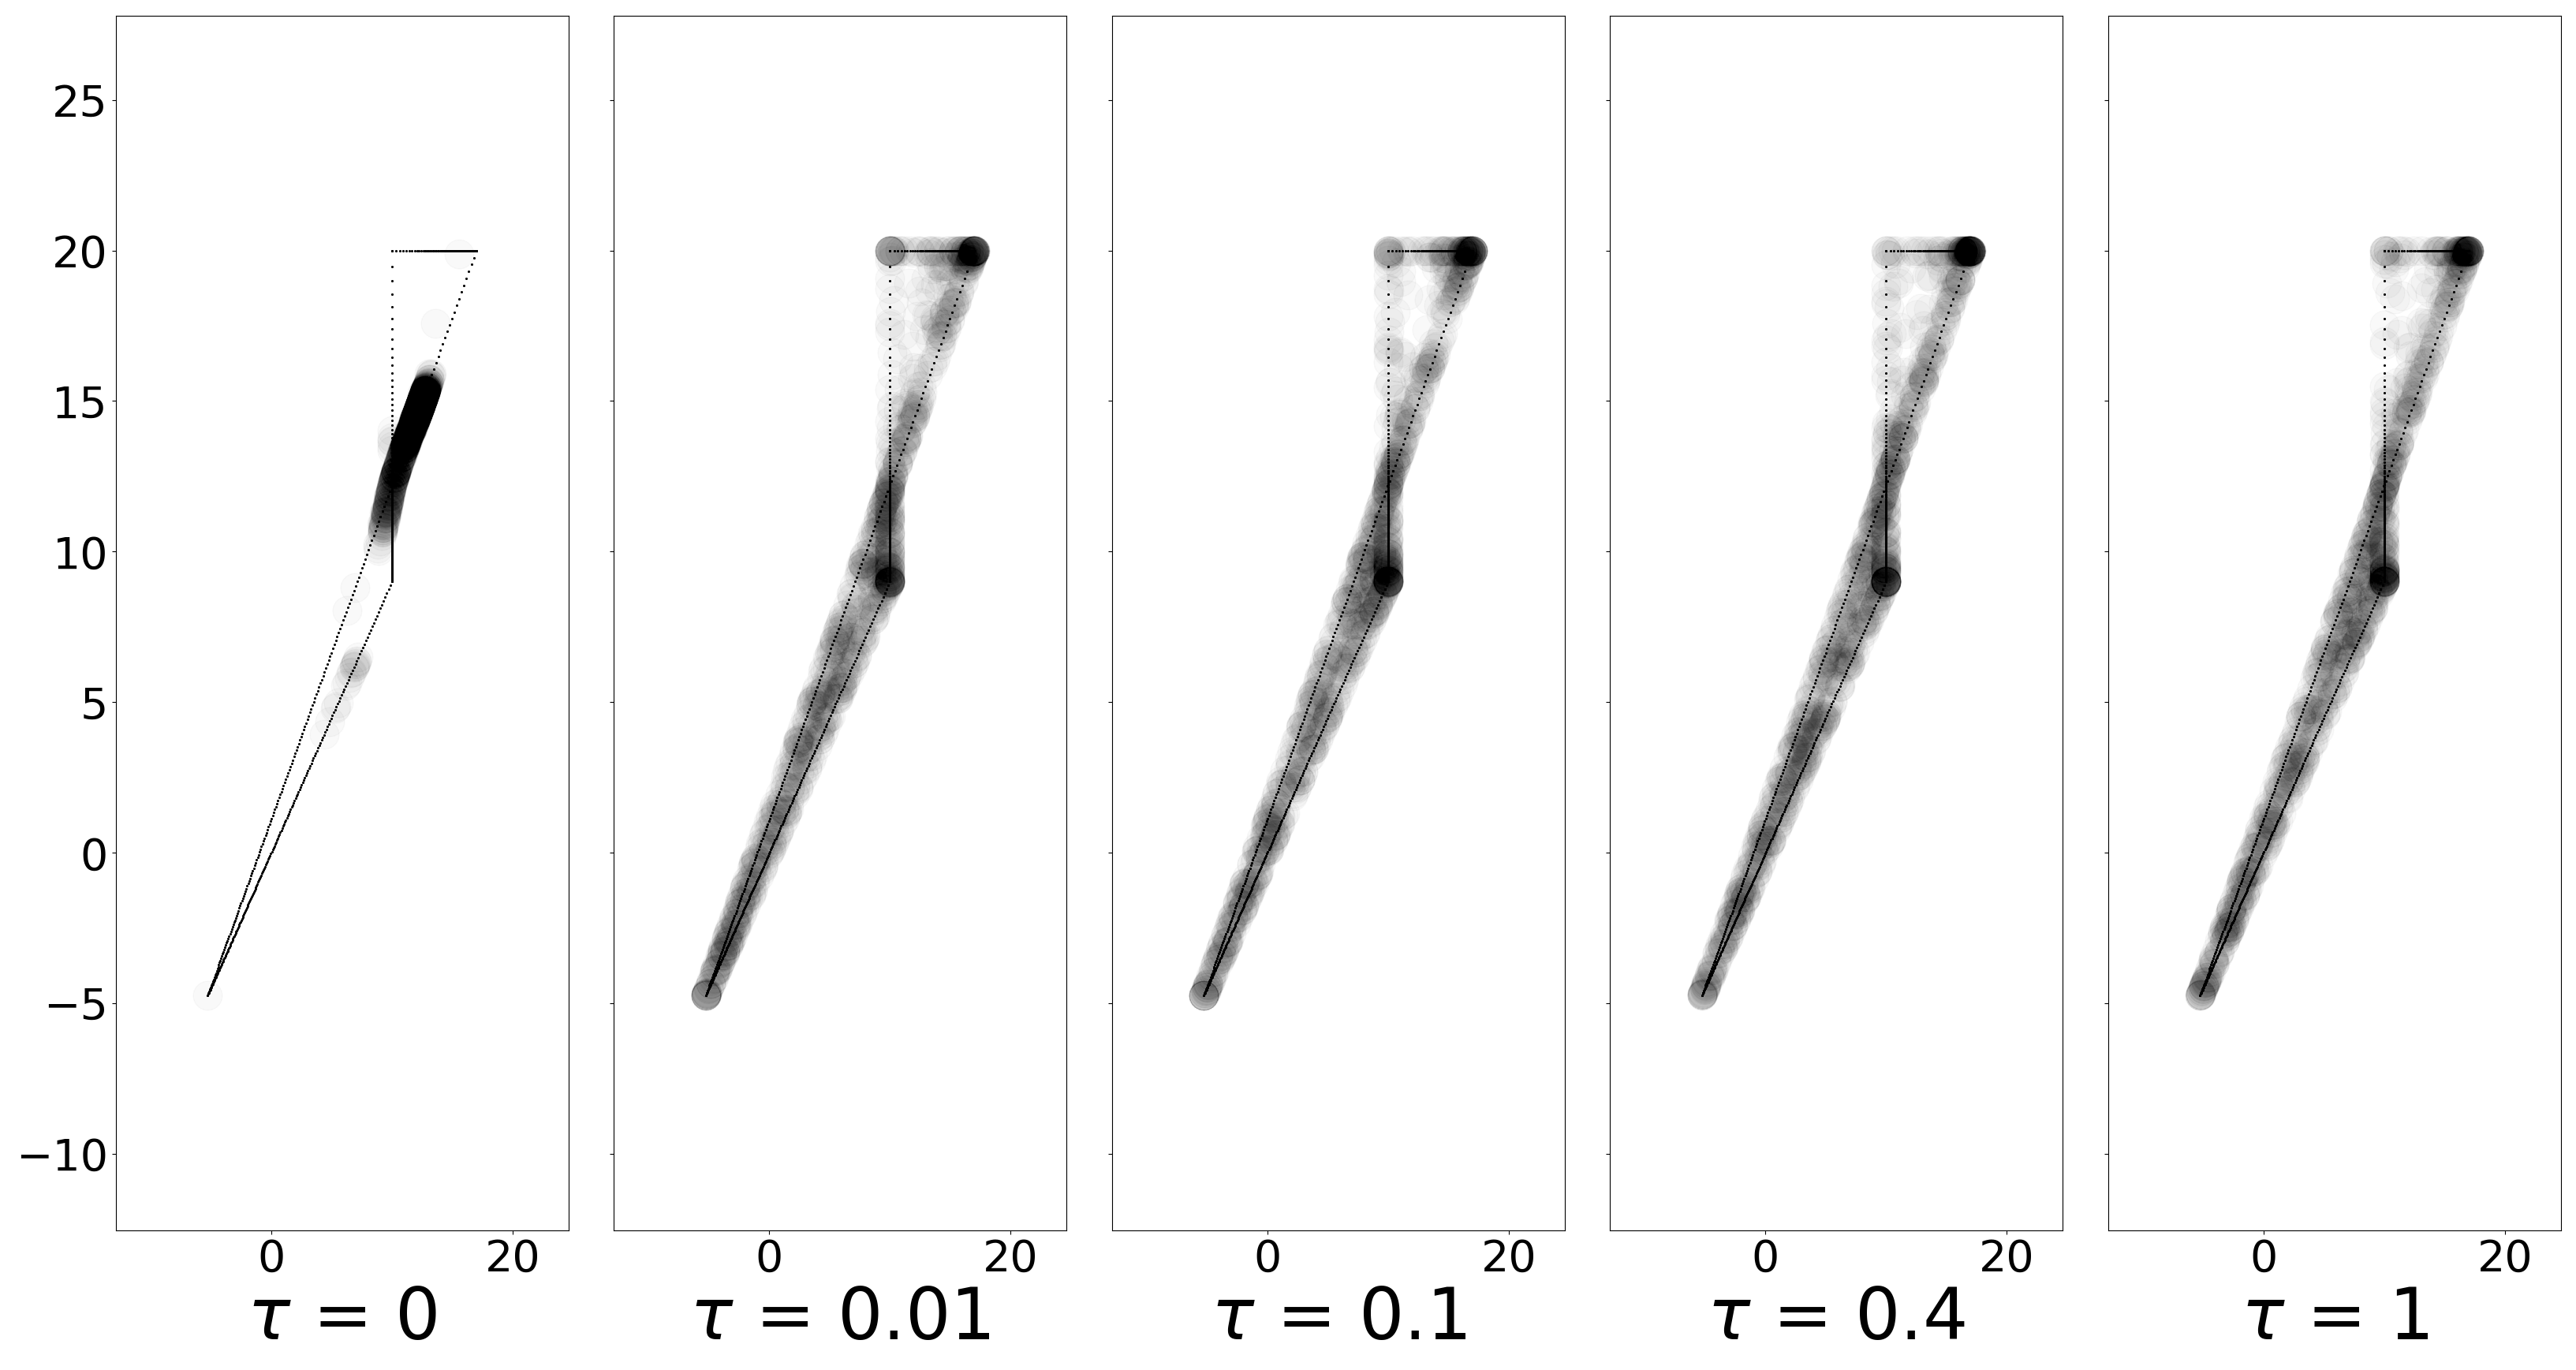
\includegraphics[width=0.8\columnwidth]{figs/continuous-switch-stay/notlearnQ/polytope_forward_optim=sgd_lr=0.005.png}
%     \caption{Forward KL.}
%     \label{fig:cont-switch-stay-forward-sgd}
%   \end{subfigure}%
%   \begin{subfigure}[b]{0.5\linewidth}
%         \centering
%         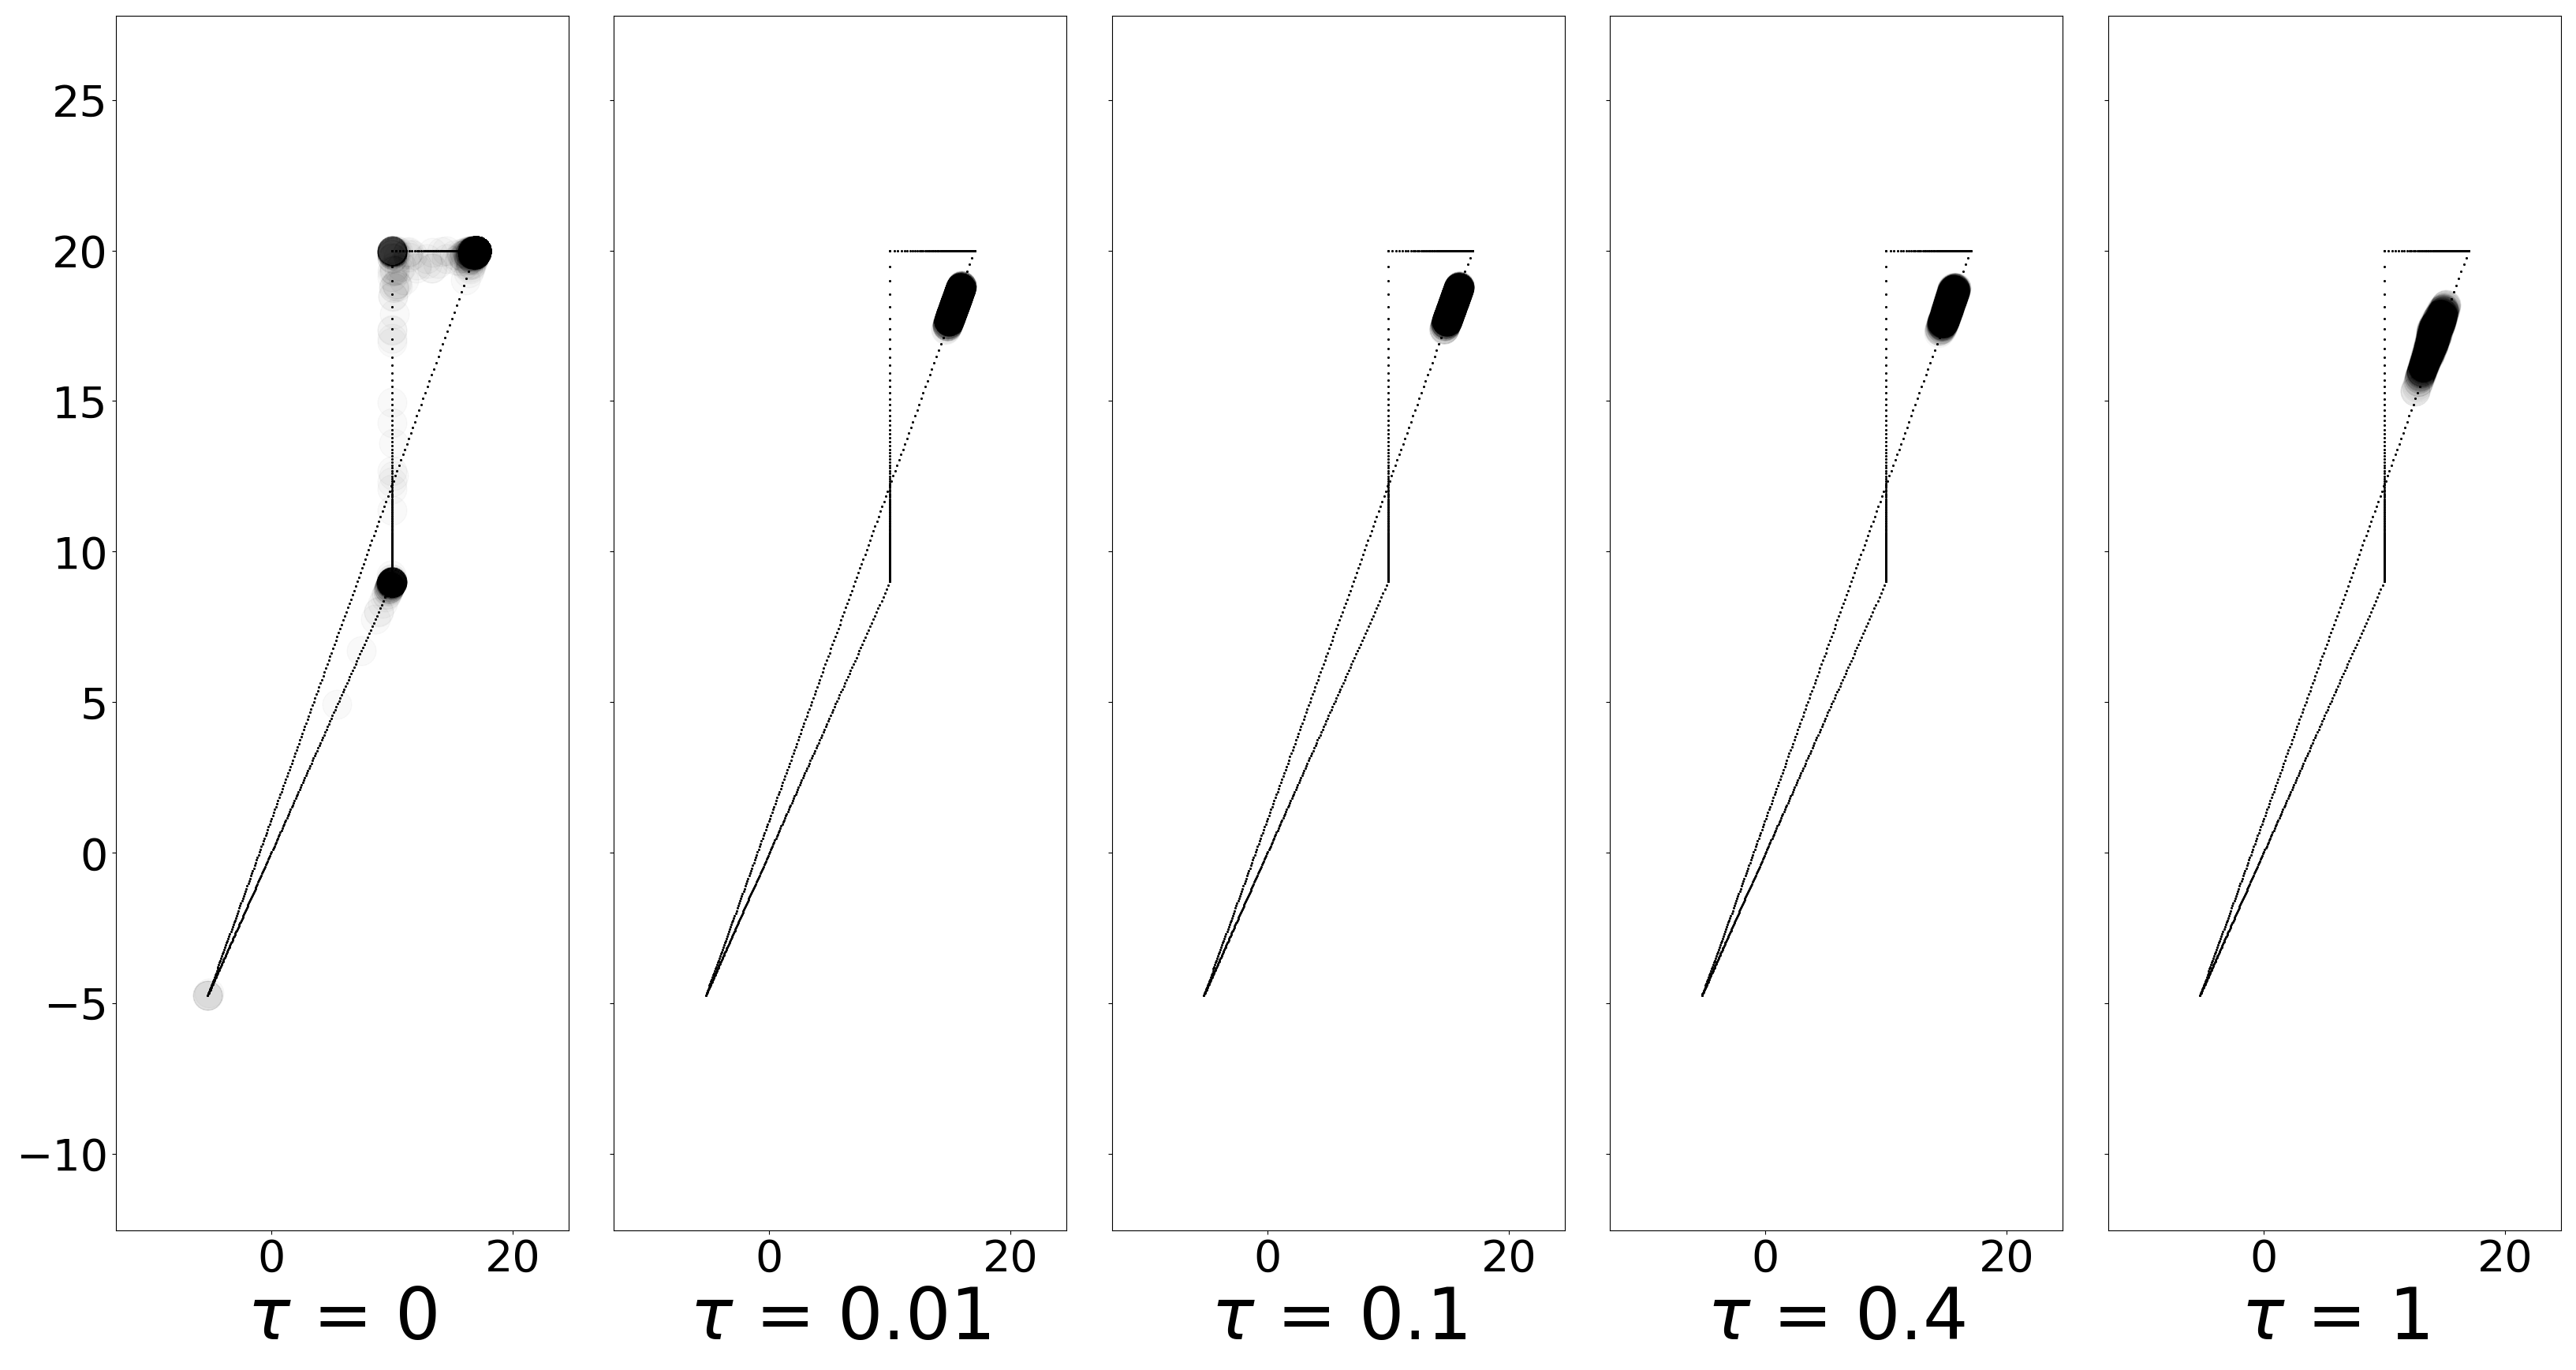
\includegraphics[width=0.8\columnwidth]{figs/continuous-switch-stay/notlearnQ/polytope_reverse_optim=sgd_lr=0.005.png}
%         \caption{Reverse KL.}
%         \label{fig:cont-switch-stay-reverse-sgd}
%   \end{subfigure}
%   \caption{Final value functions on continuous version of switch-stay after 500 gradient steps, $\gamma = 0.9$. Using SGD.}
% \end{figure}

% \clearpage 
% \textbf{Discrete Switch-Stay}

% \begin{figure}[!htb]
%   \centering
%   \begin{subfigure}[b]{0.5\linewidth}
%     \centering
%     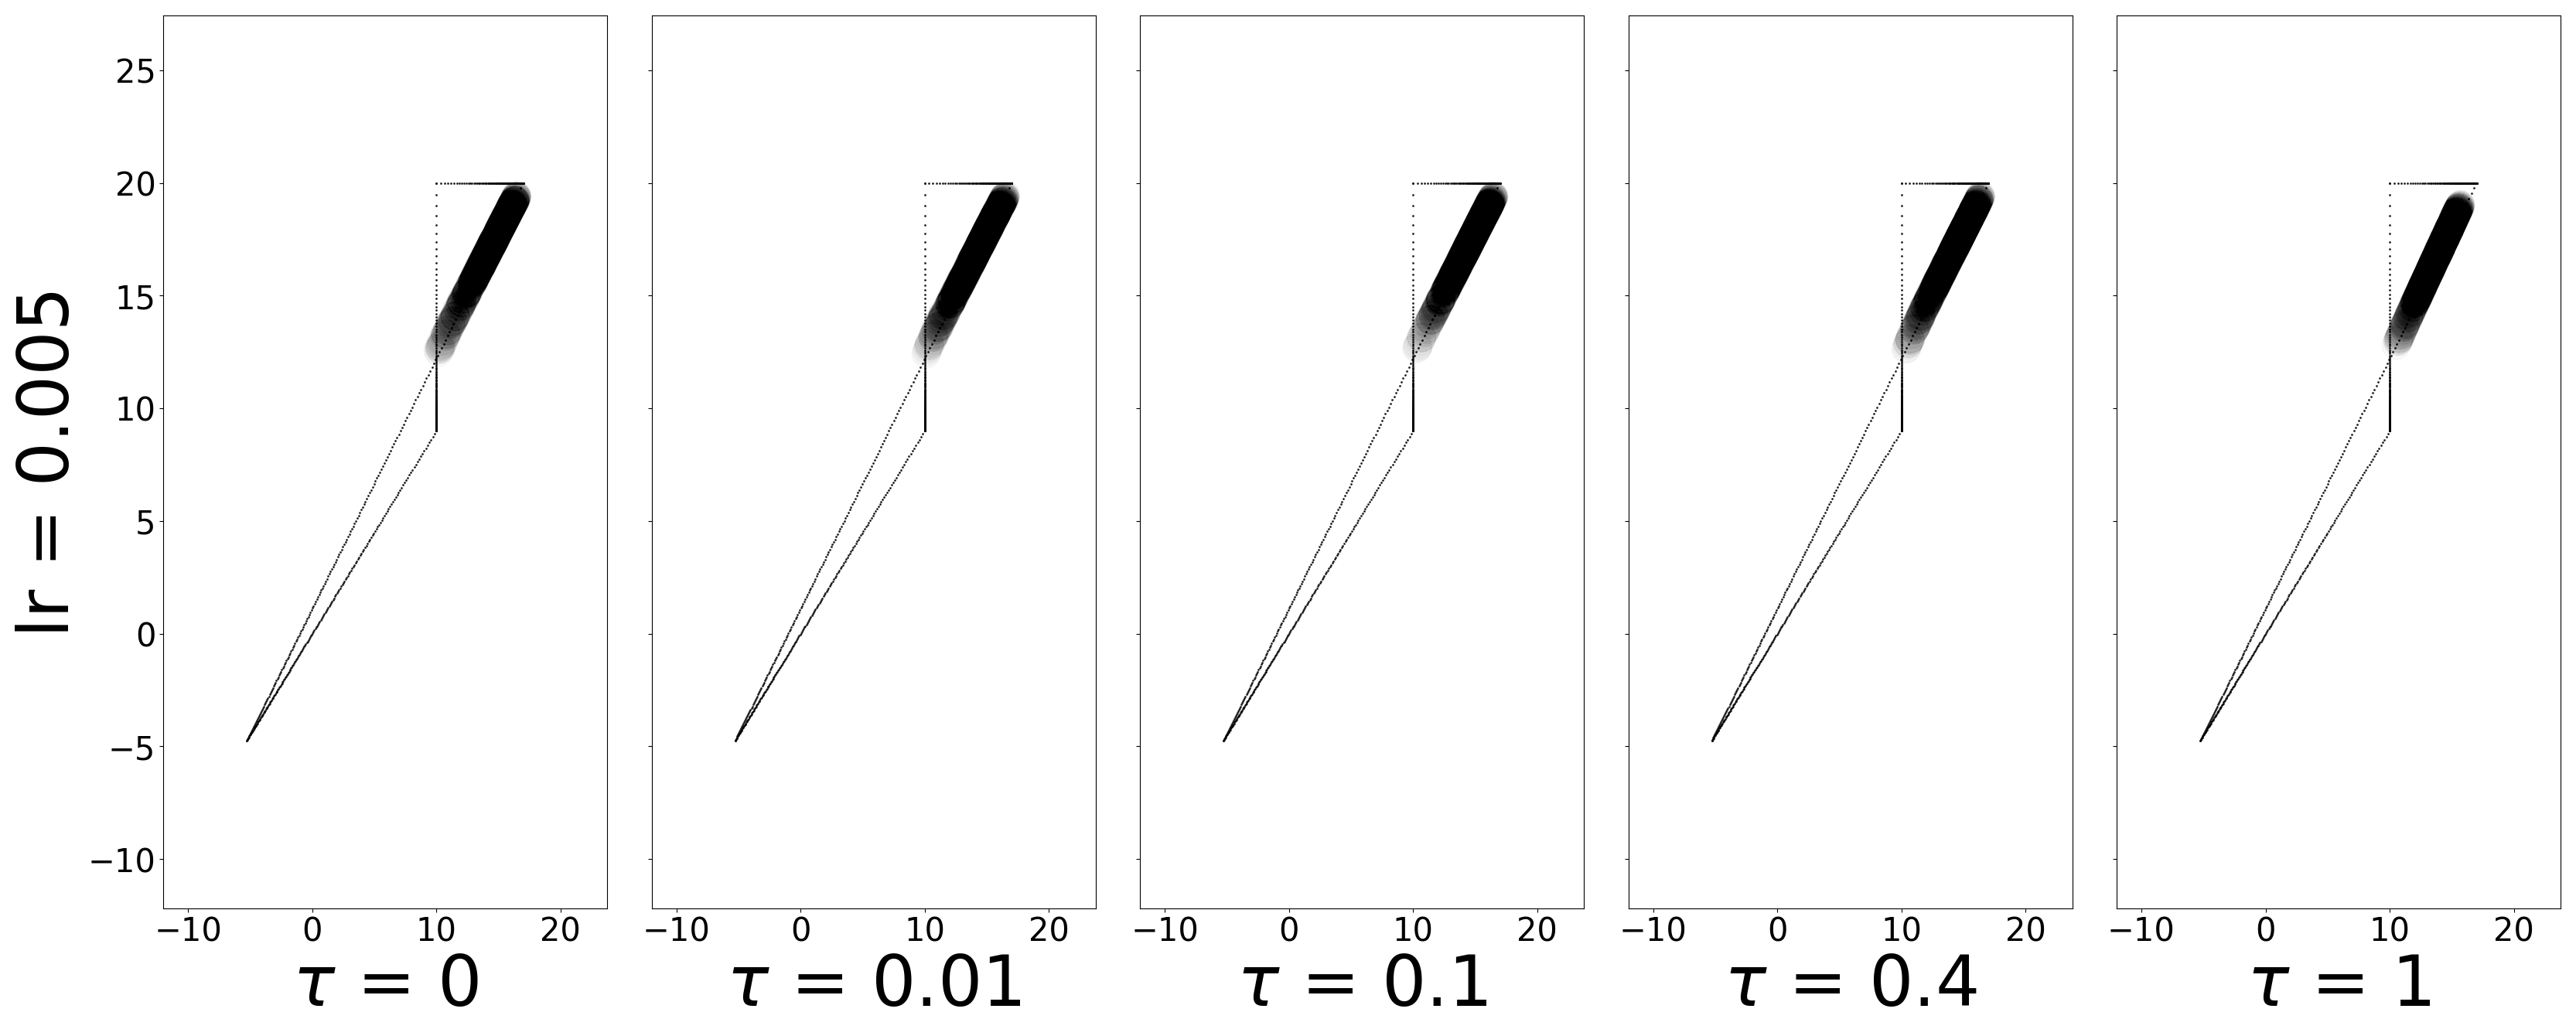
\includegraphics[width=0.8\columnwidth]{figs/switch-stay/notlearnQ/polytope_forward_optim=adam.png}
%     \caption{Forward KL.}
%     \label{fig:switch-stay-forward-adam}
%   \end{subfigure}%
%   \begin{subfigure}[b]{0.5\linewidth}
%         \centering
%         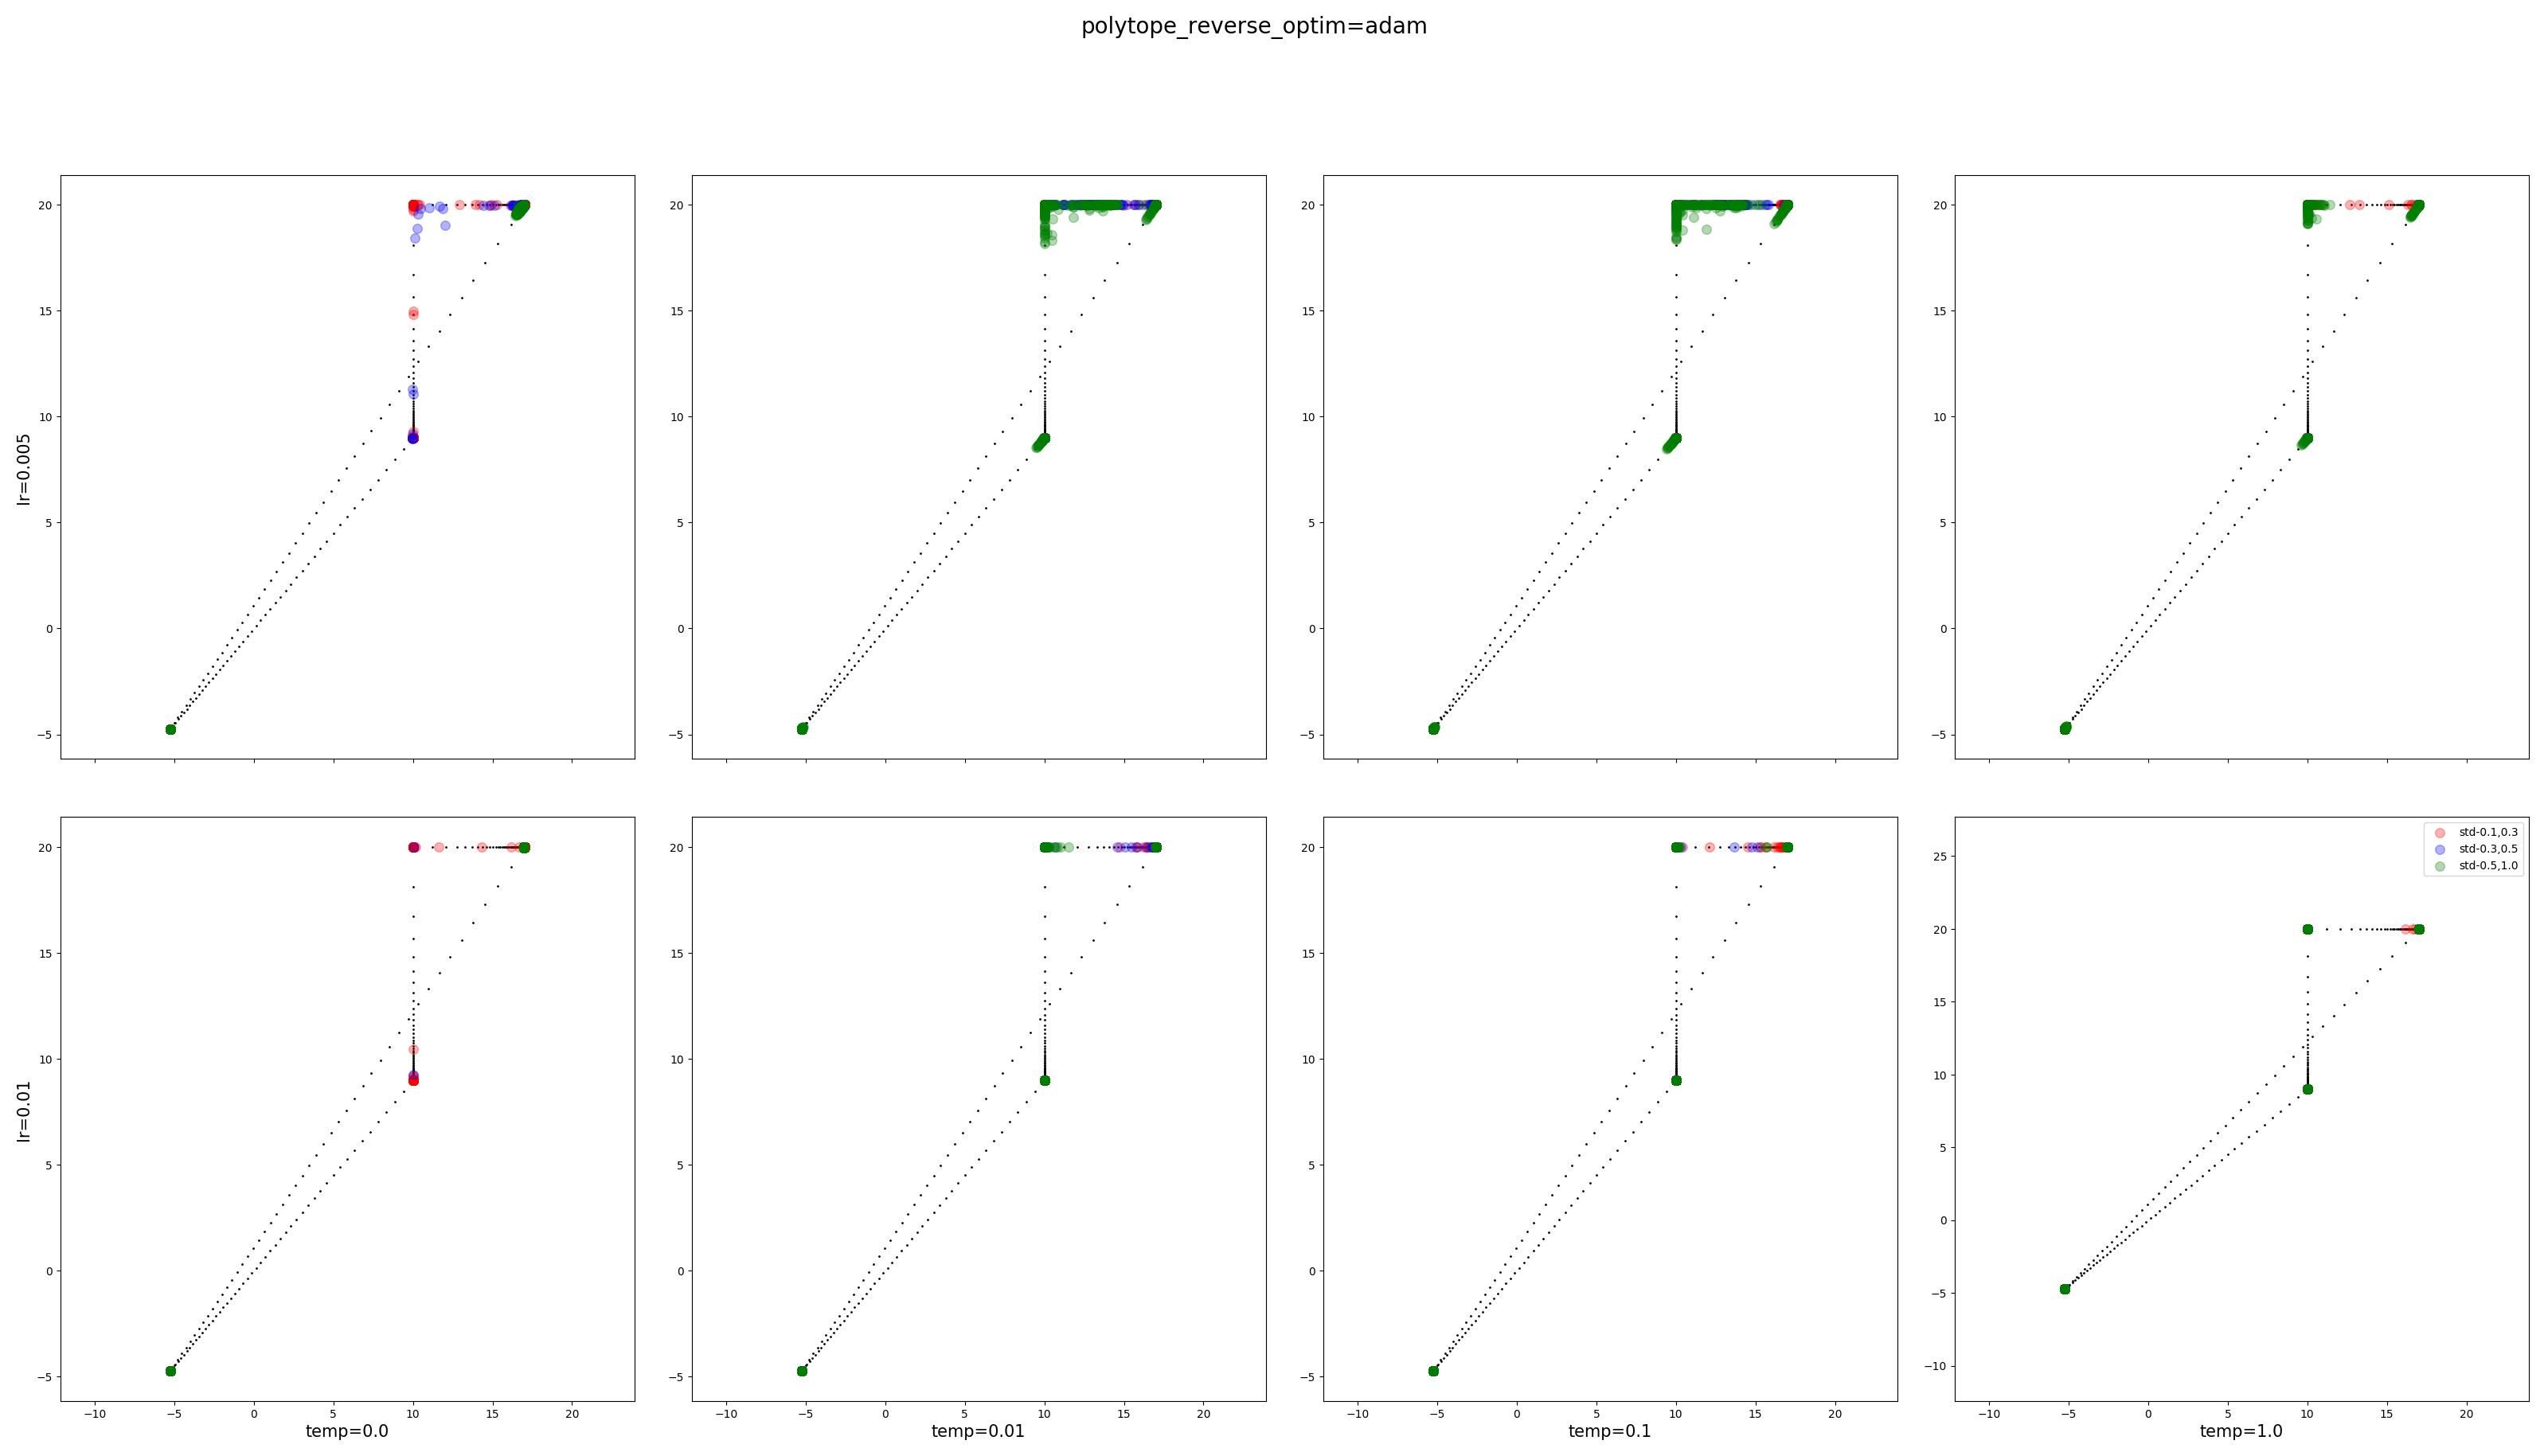
\includegraphics[width=0.8\columnwidth]{figs/switch-stay/notlearnQ/polytope_reverse_optim=adam.png}
%         \caption{Reverse KL.}
%         \label{fig:switch-stay-reverse-adam}
%   \end{subfigure}
%   \caption{Final value functions on discrete version of switch-stay after 500 gradient steps, $\gamma = 0.9$. Using Adam.}
% \end{figure}


% \begin{figure}[!htb]
%   \centering
%   \begin{subfigure}[b]{0.5\linewidth}
%     \centering
%     \includegraphics[width=0.8\columnwidth]{figs/switch-stay/notlearnQ/polytope_forward_optim=rmsprop.png}
%     \caption{Forward KL.}
%     \label{fig:switch-stay-forward-rmsprop}
%   \end{subfigure}%
%   \begin{subfigure}[b]{0.5\linewidth}
%         \centering
%         \includegraphics[width=0.8\columnwidth]{figs/switch-stay/notlearnQ/polytope_reverse_optim=rmsprop.png}
%         \caption{Reverse KL.}
%         \label{fig:switch-stay-reverse-rmsprop}
%   \end{subfigure}
%   \caption{Final value functions on discrete version of switch-stay after 500 gradient steps, $\gamma = 0.9$. Using RMSprop.}
% \end{figure}

% \begin{figure}[!htb]
%   \centering
%   \begin{subfigure}[b]{0.5\linewidth}
%     \centering
%     \includegraphics[width=0.8\columnwidth]{figs/switch-stay/notlearnQ/polytope_forward_optim=sgd.png}
%     \caption{Forward KL.}
%     \label{fig:switch-stay-forward-sgd}
%   \end{subfigure}%
%   \begin{subfigure}[b]{0.5\linewidth}
%         \centering
%         \includegraphics[width=0.8\columnwidth]{figs/switch-stay/notlearnQ/polytope_reverse_optim=sgd.png}
%         \caption{Reverse KL.}
%         \label{fig:switch-stay-reverse-sgd}
%   \end{subfigure}
%   \caption{Final value functions on discrete version of switch-stay after 500 gradient steps, $\gamma = 0.9$. Using SGD.}
% \end{figure}
\end{document}